%% GABARIT POUR MÉMOIRE STANDARD
%%
%% Consulter la documentation de la classe ulthese pour une
%% description détaillée de la classe, de ce gabarit et des options
%% disponibles.
%%
%% [Ne pas hésiter à supprimer les commentaires après les avoir lus.]
%%
%% Déclaration de la classe avec le type de grade
%%   [l'un de MATDR, MArch, MA, LLM, MErg, MMus, MPht, MSc, MScGeogr,
%%    MServSoc, MPsEd]
%% et les langues les plus courantes. Le français sera la langue par
%% défaut du document.
\documentclass[MSc,english,french]{ulthese}
  %% Encodage utilisé pour les caractères accentués dans les fichiers
  %% source du document. Les gabarits sont encodés en UTF-8. Inutile
  %% avec XeLaTeX, qui gère Unicode nativement.
  \ifxetex\else \usepackage[utf8]{inputenc} \fi

  %% Charger ici les autres paquetages nécessaires pour le document.
  %% Quelques exemples; décommenter au besoin.
  \usepackage{amsmath}       % recommandé pour les mathématiques
  %\usepackage{icomma}        % gestion de la virgule dans les nombres

  %% Utilisation d'une autre police de caractères pour le document.
  %% - Sous LaTeX
  %\usepackage{mathpazo}      % texte et mathématiques en Palatino
  %\usepackage{mathptmx}      % texte et mathématiques en Times
  %% - Sous XeLaTeX
  %\setmainfont{TeX Gyre Pagella}      % texte en Pagella (Palatino)
  %\setmathfont{TeX Gyre Pagella Math} % mathématiques en Pagella (Palatino)
  %\setmainfont{TeX Gyre Termes}       % texte en Termes (Times)
  %\setmathfont{TeX Gyre Termes Math}  % mathématiques en Termes (Times)
  
  %DIF PREAMBLE EXTENSION ADDED BY LATEXDIFF
  %DIF UNDERLINE PREAMBLE %DIF PREAMBLE
  \RequirePackage[normalem]{ulem} %DIF PREAMBLE
  \RequirePackage{color}\definecolor{RED}{rgb}{1,0,0}\definecolor{BLUE}{rgb}{0,0,1} %DIF PREAMBLE
  \providecommand{\DIFadd}[1]{{\protect\color{blue}\uwave{#1}}} %DIF PREAMBLE
  \providecommand{\DIFdel}[1]{{\protect\color{red}\sout{#1}}}                      %DIF PREAMBLE
  %DIF SAFE PREAMBLE %DIF PREAMBLE
  \providecommand{\DIFaddbegin}{} %DIF PREAMBLE
  \providecommand{\DIFaddend}{} %DIF PREAMBLE
  \providecommand{\DIFdelbegin}{} %DIF PREAMBLE
  \providecommand{\DIFdelend}{} %DIF PREAMBLE
  %DIF FLOATSAFE PREAMBLE %DIF PREAMBLE
  \providecommand{\DIFaddFL}[1]{\DIFadd{#1}} %DIF PREAMBLE
  \providecommand{\DIFdelFL}[1]{\DIFdel{#1}} %DIF PREAMBLE
  \providecommand{\DIFaddbeginFL}{} %DIF PREAMBLE
  \providecommand{\DIFaddendFL}{} %DIF PREAMBLE
  \providecommand{\DIFdelbeginFL}{} %DIF PREAMBLE
  \providecommand{\DIFdelendFL}{} %DIF PREAMBLE
  %DIF END PREAMBLE EXTENSION ADDED BY LATEXDIFF
  
 \usepackage{graphicx}
 \usepackage{subcaption}
 \usepackage{amsfonts}
 \usepackage{float} 
  
 % Section reference
 \usepackage{hyperref}

 % Networks
 \def\layersep{2cm}
 \usepackage{tikz}
 \usepackage{verbatim}
 \usetikzlibrary{decorations.pathreplacing}
 \usetikzlibrary{decorations.pathreplacing}
 \usetikzlibrary{shapes.geometric}
	
 %Tableau
 \usepackage{array,multirow,makecell}
 \usepackage{xcolor,colortbl}
 \definecolor{Gray}{gray}{0.85}
 \newcolumntype{a}{>{\columncolor{white}}c}
 \setlength{\aboverulesep}{0pt}
 \setlength{\belowrulesep}{0pt}
 
 \newcommand{\PLH}{{\mkern-2mu\times\mkern-2mu}}
 \newcommand\norm[1]{\left\lVert#1\right\rVert}

	% Algorithms
	\usepackage[ruled,vlined]{algorithm2e}

  %% Options de mise en forme du mode français de babel. Consulter la
  %% documentation du paquetage babel pour les options disponibles.
  %% Désactiver (effacer ou mettre en commentaire) si l'option
  %% 'nobabel' est spécifiée au chargement de la classe.
  \frenchbsetup{%
    StandardItemizeEnv=true,       % format standard des listes
    ThinSpaceInFrenchNumbers=true, % espace fine dans les nombres
    og=«, fg=»                     % caractères « et » sont les guillemets
  }

  %% Style de la bibliographie.
 \bibliographystyle{apalike}

  %% Composition de la page frontispice. Remplacer les éléments entre < >.
  %% Supprimer les caractères < >. Couper un long titre ou un long
  %% sous-titre manuellement avec \\.
  \titre{<Titre principal>}
  % \titre{Ceci est un exemple de long titre \\
  %   avec saut de ligne manuel}
  % \soustitre{Sous-titre le cas échéant}
  % \soustitre{Ceci est un exemple de long sous-titre \\
  %   avec saut de ligne manuel}
  \auteur{<Prénom Nom>}
  \programme{Maîtrise en <discipline> <-- majeure, s'il y a lieu>}
  \direction{<Prénom Nom>, <directeur ou directrice> de recherche}
  % \codirection{<Prénom Nom>, <codirecteur ou codirectrice> de recherche}
  % \codirection{<Prénom Nom>, <codirecteur ou codirectrice> de recherche \\
  %              <Prénom Nom>, <codirecteur ou codirectrice> de recherche}

  %% Les commandes ci-dessous servent uniquement pour la création
  %% d'une page de titre (interdite lors du dépôt à la FESP).
  % \annee{<20xx>}

\begin{document}

\frontmatter                    % pages liminaires

%\frontispice                    % production de la page frontispice

\chapter*{Résumé}             % ne pas numéroter
\label{chap:resume}           % étiquette pour renvois
\phantomsection\addcontentsline{toc}{chapter}{\nameref{chap:resume}} % inclure dans TdM


Dans ce mémoire, nous proposons une méthodologie qui permet de détecter des anomalies parmi un ensemble de données complexes, plus particulièrement des images. Pour y arriver, nous utilisons un type spécifique de réseau de neurones, soit un autoencodeur variationnel (VAE). Cette approche non-supervisée d'apprentissage profond nous permet d'obtenir une représentation plus simple de nos données sur laquelle nous appliquerons une mesure de distance de Kullback-Leibler nous permettant de discriminer les anomalies des observations "normales". Pour déterminer si une image nous apparaît comme "anormale", notre approche se base sur une proportion d'observations à filtrer, ce qui est plus simple et intuitif à établir qu'un seuil sur la valeur même de la distance. En utilisant notre méthodologie sur des images réelles, nous avons démontré que nous pouvons obtenir des performances de détection d'anomalies supérieures en termes d'aire sous la courbe (ROC), de précision et de rappel par rapport à d'autres approches non-supervisées. De plus, nous avons montré que la simplicité de l'approche par niveau de filtration permet d'adapter facilement la méthode à des jeux de données ayant différents niveaux de contamination d'anomalies.
                % résumé français
\chapter*{Abstract}             % ne pas numéroter
\label{chap:abstract}           % étiquette pour renvois
\phantomsection\addcontentsline{toc}{chapter}{\nameref{chap:abstract}} % inclure dans TdM

\begin{otherlanguage*}{english}
In this master's thesis, we propose a methodology that aims to detect anomalies among complex data, such as images. In order to do that, we use a specific type of neural network called the varitionnal autoencoder (VAE). This non-supervised deep learning approach allows us to obtain a simple representation of our data on which we then use the Kullback-Leibler distance to discriminate between anomalies and "normal" observations. To determine if an image is considered as "abnormal", our approach is based on a proportion of observations to be filtered, which is easier and more intuitive to establish compared to applying a threshold based on the value of a distance metric. By using our methodology on real complex images, we can obtain superior anomaly detection performances in terms of area under the curve (AUC), precision and recall compared to other non-supervised methods. Moreover, we demonstrate that the simplicity of our filtration level allows us to easily adapt the method to datasets having different levels of anomaly contamination.
\end{otherlanguage*}              % résumé anglais
\cleardoublepage

\tableofcontents                % production de la TdM
\cleardoublepage

\listoftables                   % production de la liste des tableaux
\cleardoublepage

\listoffigures                  % production de la liste des figures
\cleardoublepage


%\epigraphe{<Texte de l'épigraphe>}{<Source ou auteur>}
%\cleardoublepage

\chapter*{Remerciements}        % ne pas numéroter
\label{chap:remerciements}      % étiquette pour renvois
\phantomsection\addcontentsline{toc}{chapter}{\nameref{chap:remerciements}} % inclure dans TdM

<Texte des remerciements en prose.>
         % remerciements

\mainmatter                     % corps du document

\chapter*{Introduction}         % ne pas numéroter
\label{chap:introduction}       % étiquette pour renvois
\phantomsection\addcontentsline{toc}{chapter}{\nameref{chap:introduction}} % inclure dans TdM


La détection d'anomalies est un sujet complexe qui a généré beaucoup de littérature en statistique,  en apprentissage machine et plus récemment en vision numérique. Il existe plusieurs applications de ces méthodes dans les domaines de la cyber-intrusion, de la finance et de l'assurance, de la médecine ou dans l'identification de dommages industriels \citep{chandola2009anomaly}. Une anomalie est définie par \cite{Zimek2017} comme un événement, une mesure ou une observation qui diffère significativement de la majorité des données. Une anomalie, également appelée une aberration, est une notion intrinsèque à plusieurs domaines reliés à l'analyse des données, car une donnée anormales ou aberrante est généralement intéressante à identifier ou retirer d'une source de données. Dans un premier temps, il peut être intéressant de l'identifier simplement parce que c'est  l'objectif poursuivi en soi. Dans un deuxième temps, il peut également être pertinent de retirer une observation anormale ou aberrante avant de réaliser une autre tâche d'apprentissage. 

Une difficulté reliée à la détection d'anomalies est qu'on doit souvent utiliser des données non étiquetées, car les anomalies sont généralement générées par des phénomènes imprévus. Cela fait en sorte qu'on doit approcher le problème de manière non-supervisée. Une autre difficulté, plus particulièrement reliée avec les approches non-supervisées, est qu'il faut généralement déterminer un seuil nous permettant de prendre une décision quant à la nature d'une donnée (anomalie ou non). Finalement, ces difficultés deviennent encore plus prononcées lorsqu'on doit traiter des données complexes, comme des images.

Dans le contexte de données à hautes dimensions, les réseaux de neurones sont couramment utilisés. En effet, leurs couches superposées peuvent partir d'une entrée complexe, comme une image, et compresser cette information vers une représentation vectorielle plus compacte et riche en informations. Les autoencodeurs sont une catégorie de réseaux de neurones fréquemment utilisés en apprentissage non-supervisé. Il existe d'ailleurs plusieurs applications d'autoencodeurs dans un contexte de détection d'anomalies, où l'erreur de reconstruction est souvent utilisée comme indicateur d'anomalie. Cependant, ces méthodes requièrent de fixer un seuil de détection, souvent sous forme de distance ou de métrique, qui peut être difficile à établir ou à expliquer. C'est d'ailleurs pour cette raison que  \cite{An2015VariationalAB} proposent de se baser sur une probabilité de reconstruction, qui est une mesure objective et ne requiert pas de seuil quelconque. Par contre, cette mesure de probabilité est basée sur la capacité de reconstruction des observations originales, ce qui peut être problématique dans le contexte d'images complexes, plutôt que sur la représentation latente, qui elle peut être beaucoup plus simple. D'autres approches, comme dans \cite{DBLP:journals/corr/abs-1802-06360} se basent plutôt sur cette représentation latente pour faire la détection d'anomalies. C'est davantage vers ce type d'approches que nous souhaitons orienter notre méthodologie. 

Dans ce mémoire, nous proposons une approche qui vise à faire la détection d'anomalies dans un ensemble de données constitué d'images. Nous proposons également de simplifier la détermination du seuil nécessaire pour conclure quelles observations sont "normales" et quelles observations sont "anormales". Avec cette contribution, nous proposons d'utiliser des méthodes existantes comme des autoencodeurs  pour encoder des structures de données complexes dans des représentations latentes qui serviront de base pour un cadre décisionnel simple et intuitif à appliquer. À partir d'autoencodeurs variationnels (VAE), nous sommes en mesure de créer ces dites représentations et de détecter les anomalies dans un ensemble d'images.          % introduction
\chapter{Contexte}     % numéroté
\label{chap:background}                   % étiquette pour renvois (à compléter!)

En premier lieu, nous allons commencer par faire une brève revue des différentes catégories  de méthodes de détection d'anomalies et de leur fonctionnement respectif. Ensuite, nous allons faire un résumé de la théorie des autoencodeurs et comment ceux-ci sont pertinents dans un contexte de détection d'anomalies. Ensuite, nous allons décrire plus en détails un type particulier d'autoencodeur utilisé dans cette étude, soit l'autoencodeur variationnel. Finalement, nous allons couvrir quelques notions de base quant aux tests d'hypothèses, un cadre statistique classique pour prendre des décisions.

\section{Les méthodes de détection d'anomalies}

Tout d'abord, il est pertinent de commencer par mentionner que toutes les méthodes de détection d'anomalies fonctionnent fondamentalement de la même manière. En effet, ces algorithmes sont en mesure de faire l'apprentissage d'un jeu de données et de stocker cette information dans un modèle d'apprentissage. En sachant ce qui est normal, il est donc également possible d'utiliser ce modèle pour évaluer ce qui est anormal en identifiant ce qui dévie de cette normalité. Le choix du modèle est cruciale, car si celui-ci ne s'ajuste pas bien aux données, il pourrait nous induire en erreur sur l'anormalité d'une observation (\cite{10.5555/3086742}). 

Pour démontrer l'importance du choix de modèle, prenons un exemple simpliste et fréquemment utilisé en pratique, soit sur la moyenne d'une loi normale à variance connue, souvent appelé le test $Z$. Dans ce test statistique, qui peut être utilisé pour de la détection d'anomalies, l'hypothèse nulle est que les données suivent une loi normale. Prenons par exemple des observations à $1$ dimension $X_1, ..., X_N$ avec une moyenne $\mu$ et un écart-type $\sigma$. La valeur $Z$ pour une observation $X_i$ est donnée par :

\begin{gather}
Z_i = \frac{|X_i-\mu|}{\sigma}.
\end{gather}

Cette valeur $Z$ nous donne en fait le nombre d'écarts-types dont une observation dévie de la moyenne. On peut généralement penser que si une observation dévie beaucoup de la moyenne, ça peut être un indicateur important d'anomalie. Dans ce cas-ci, on utilise généralement la règle du pouce $Z_i \ge 3$ comme indicateur d'anomalie. En d'autres mots, une observation est improbable, ou potentiellement anormale, si elle se situe à plus ou moins 3 écarts-types de la moyenne. Dans la figure \ref{fig:ZTest} (image de gauche), on peut voir que cela est plutôt vrai sachant que les données ont été simulées à partir d'une loi $N(0, 2)$. Dans ce cas précis, l'intervalle correspondant à notre règle du pouce est l'intervalle $[-6, 6]$. Cela fonctionne bien puisque notre choix de modèle représente bien les données. Comme contre exemple, supposons que nos données proviennent plutôt d'une loi à queue lourde, comme la loi standard Cauchy. En simulant $5000$ observations de cette loi, nous obtenons une moyenne empirique de $-1.6$ et un écart-type empirique de $160.2$. C'est donc dire que l'intervalle défini avec le modèle précédent serait de $[-482.2, 479]$. On peut voir (figure \ref{fig:ZTest}, image de droite), que plusieurs observations ne sont pas considérées comme des anomalies, alors que leur fréquence relative est pourtant très faible.


\begin{figure}[htb]
	\centering
	\begin{subfigure}{6cm}
		\centering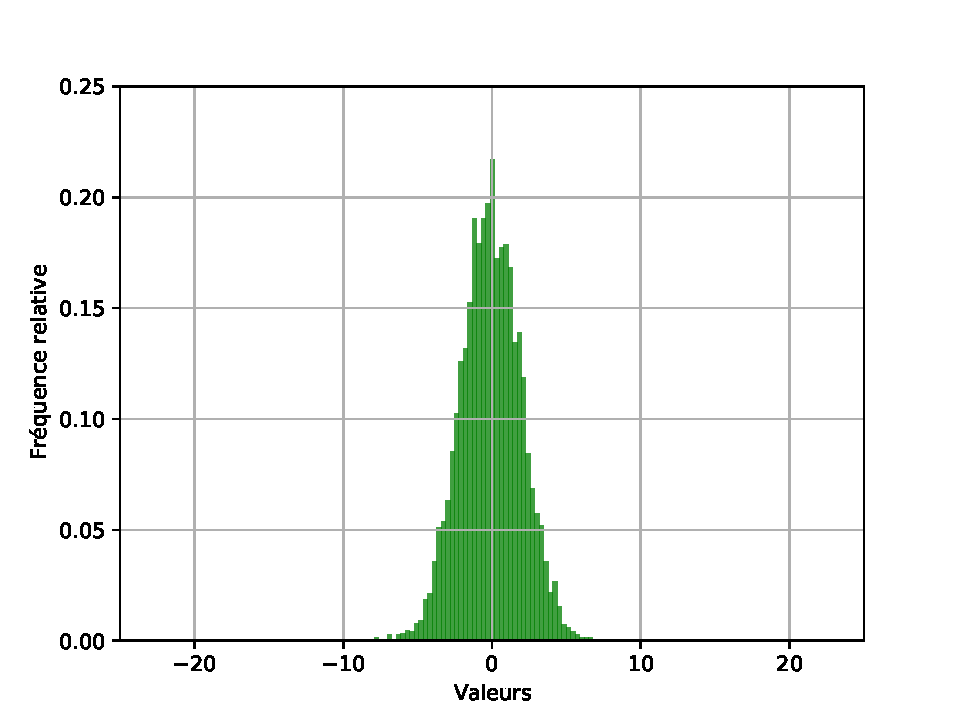
\includegraphics[width=6cm]{images/histogram-normal-ztest}
		\caption{Distribution normale}
	\end{subfigure}
	\begin{subfigure}{6cm}
		\centering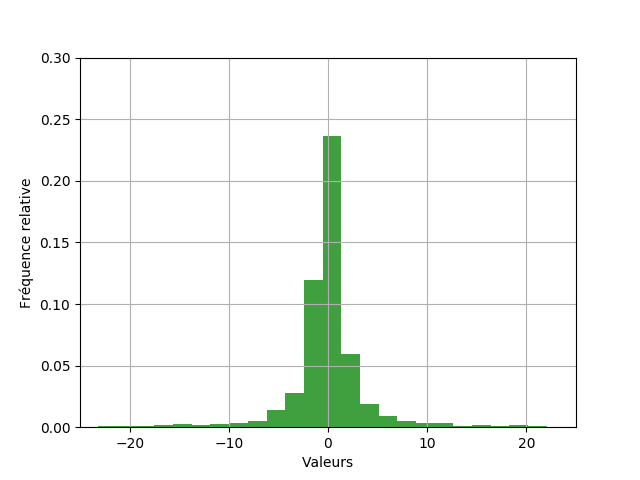
\includegraphics[width=6cm]{images/histogram-cauchy-ztest}
		\caption{Distribution standard Cauchy}
	\end{subfigure}
	\caption{Distribution de 5000 simulations d'une loi normale et d'une loi standard Cauchy}
	\label{fig:ZTest}
\end{figure}

L'exemple du test $Z$ illustre simplement le fait que le choix du modèle aura un impact important dans la détection d'anomalies. Au final, la pertinence du modèle choisi sera étroitement lié à la nature des données. Il existe plusieurs catégories d'algorithmes de détection d'anomalies. Dans \cite{10.5555/3086742}, 4 de ces approches nous apparaissent comme particulièrement intéressantes à survoler.

\subsection{Analyse des valeurs extrêmes}

La détection d'anomalies via l'analyse des valeurs extrêmes est probablement une des approches les plus simples. Dans un cas à une seule dimension, les anomalies sont définies comme les valeurs très grandes ou très faibles. On s'intéresse donc à la queue d'une distribution, comme dans l'exemple avec le test $Z$ présenté plus tôt. Cette approche vient légèrement à l'encontre de la définition d'une anomalie présentée plus tôt où l'accent est plutôt mis sur le fait qu'une anomalie diffère de la majorité des données. Cette dernière définition fait davantage référence à une notion de probabilité.

Bien que l'analyse des valeurs extrêmes ne soit pas la méthode la plus utilisée en pratique pour identifier des anomalies, elle fait souvent partie intégrante de plusieurs autres méthodes. En effet, l'analyse de valeurs extrêmes est souvent utilisée comme étape finale de plusieurs autres algorithmes. C'est d'ailleurs ce qui permet généralement de déterminer ce qui dévie d'une certaine normalité, via une valeur unidimensionnelle comme un score d'anomalie ou une distance.


\subsection{Les modèles probabilistes}

L'élément clé des approches basées sur des modèles probabilistes  est qu'on fait une hypothèse sur la distribution des données. Ensuite, on ajuste le modèle statistique correspondant à cette hypothèse sur les données en faisant l'apprentissage des paramètres du modèle. Un exemple classique pourrait être d'ajuster un mélange de $k$ lois normales. Avec ce modèle, on fait l'hypothèse que chaque observation provient d'un des $k$ groupes de la loi mélange. On peut faire l'apprentissage des paramètres du modèle avec l'algorithme \textit{expectation-maximization (EM)}. Par la suite, on peut évaluer l'anormalité d'une observation en se basant sur la probabilité de cette instance selon notre modèle ajusté. Ce type d'approche a l'avantage de pouvoir s'appliquer assez facilement à plusieurs types de données. Par contre, le désavantage est que l'on doit faire une hypothèse quant à la distribution des données, qui peut parfois être inadéquate. Certains jeux de données peuvent difficilement être représenté par une distribution connue, ce qui peut mener à un mauvais ajustement du modèle et ainsi tirer de mauvaises conclusions quant à la nature d'une observation.

\subsection{Les modèles linéaires et non-linéaires} \label{soussec:linear}

Ce type d'approche est basé sur l'apprentissage d'un espace à plus petites dimensions via un modèle linéaire ou non-linéaire. Un exemple classique est l'utilisation d'une régression linéaire. Par exemple, dans un cas d'une régression linéaire à 2 variables explicatives, l'apprentissage d'une variable réponse $y_i$ est donnée par l'équation \ref{eq_reg}. Dans ce cas-ci, on utilise généralement la méthode des moindres carrés pour trouver les paramètres optimaux du modèle, soit les paramètres $\beta_0$, $\beta_1$ et $\beta_2$.

\begin{gather}  \label{eq_reg}
y_i = \beta_0 + \beta_{1} x_{1,i} + \beta_2 x_{2,i} + \epsilon_{i} \qquad \forall i \in {1,...,N}
\end{gather}

Les estimations de ces paramètres, soit $\hat{\beta_0}$, $\hat{\beta_1}$ et $\hat{\beta_2}$, nous permettent d'estimer la variable réponse $\hat{y_i}$: 

\begin{gather}  \label{eq_reghat}
\hat{y_i} = \hat{\beta_0} + \hat{\beta_{1}} x_{1,i} + \hat{\beta_2} x_{2,i} \qquad \forall i \in {1,...,N}
\end{gather}

On peut ensuite utiliser l'erreur de prédiction comme indicateur d'anomalie. Cette erreur de prédiction, défini comme $\hat{y_i} - y_i$, est également appelée erreur de reconstruction. La prémisse de base est que si le modèle est en mesure de bien ajuster les données, les observations normales devraient être bien reconstruites par le modèle. À l'inverse, les observations anormales devraient être mal reconstruites par le modèle.  On peut d'ailleurs ce servir encore une fois de l'analyse des cas extrêmes pour reconnaître les erreurs les plus importantes, et par le fait même, les anomalies.
 
Un autre exemple classique dans cette catégorie d'approches est l'utilisation d'une analyse en composante principale (ACP). En effet, cette technique de réduction de dimensionnalité permet de transformer les données vers un espace où les variables sont décorrélées et où l'utilisation d'un sous-ensemble de ces variables latentes peut être suffisant pour expliquer une bonne partie de la variabilité des données originales. La transformation permettant d'obtenir un espace latent à $k$ dimensions est donnée par l'équation \ref{eq_pca1}.
 
 \begin{gather}  \label{eq_pca1}
 Z = XV
 \end{gather}
 
Dans l'équation \ref{eq_pca1}, $X$ est une matrice $n \times p$ représentant les données initiales et où le vecteur de moyennes $\boldsymbol{\mu}$, calculé sur chaque colonne, a été soustrait à la matrice originale. $X$ est donc la matrice centrée des données initiales. $V$ représente une matrice $p \times k$, où $k < p$, de  vecteurs propres correspondant aux valeurs propres les plus élevées de la matrice de corrélation $\Sigma$. La valeur $k$ signifie qu'on conserve seulement $k$ variables latentes, ou également appelées composantes principales. La reconstruction de cet espace latent à $k$ dimensions peut ensuite être retrouvé par l'équation \ref{eq_pca2}. 
 
  \begin{gather}  \label{eq_pca2}
 \hat{X} = ZV^\top + \boldsymbol{\mu}
 \end{gather}
 
La projection de cet espace latent vers l'espace original défini par l'équation \ref{eq_pca2} permet d'obtenir une erreur de reconstruction. Celle-ci est peut être obtenue par une fonction appliquée entre $\hat{X}$ et $X$. Par exemple, on pourrait prendre la distance quadratique entre chaque instances de $\hat{X}$ et $X$ et ainsi obtenir $n$ erreurs de reconstruction. Cette erreur de reconstruction peut être utilisée pour trouver les observations qui dévie de la normalité du modèle de la même manière qu'avec une régression linéaire.
  
Cette catégorie d'approches de détection d'anomalies a le potentiel de mieux s'adapter à des données où il n'y a pas de distribution connue. La régression linéaire est un exemple de modèle linéaire, mais on pourrait également utiliser un modèle plus complexe qui permet de capture des non-linéarités. Par exemple, il est possible d'utiliser des réseaux de neurones pour faire l'apprentissage des données vers un espace à plus basse dimension. Le désavantage avec de telles approches est qu'on peut perdre la notion d'interpretabilité. Dans certains exemples d'applications, il peut être intéressant de savoir quelles raisons expliquent la présence d'une anomalie dans les données.

\subsection{Les méthodes basées sur les distances}

Cette catégorie de méthodes de détection d'anomalie est basée sur l'idée de trouver les observations qui sont isolées de la majorité des autres observations. Cela est généralement quantifié par des mesures de distances ou de dissimilarités. Parmi ces méthodes, on peut retrouver 3 sous-catégories fréquemment utilisées en pratique: les regroupements (\textit{clustering}), les méthodes de densité et les méthodes des plus proches voisin.

Dans le cas des regroupements et des méthodes de densité, l'objectif est de trouver des zones de l'espace qui caractérisent le jeu de données. Les anomalies sont généralement identifiées en considérant les observations qui ne font pas parties de ces zones. Dans le cas spécifique des regroupements, on fait un séparation de l'espace qui est basée sur les observations elles-mêmes. Si on prend comme exemple l'algorithme de regroupement $k$-moyennes, on peut évaluer le score d'anomalie d'une observation en prenant la distance minimale d'un centroïde trouvé pendant l'ajustement du modèle.

Dans les méthodes de densité, plutôt que séparer l'espace par l'entremise observations, on sépare directement des zones de cette espace. Ensuite, on évalue la densité des observations dans une zone selon le nombre d'observations dans cette même zone. Le fait de séparer l'espace des données nous permet de mieux quantifier la densité d'un point, peu importe son emplacement dans l'espace. Un exemple simple serait d'utiliser la méthode de l'histogramme afin de compartimenter l'espace en plusieurs sous-espaces et ensuite évaluer la densité d'une région par le nombre d'observations s'y retrouvant. Ce genre d'approche a généralement l'avantage d'être interprétable, car on peut savoir exactement pourquoi une observation fait partie d'un sous-ensemble ayant une faible densité. Prenons un exemple simple à seulement 2 dimensions où on retrouve le poids et la grandeur d'une personne. En séparant l'espace en différentes régions, on réalise que seulement très peu de personne ont un poids inférieur à 45 kg et une grandeur supérieur à 1.80 m. Ainsi, on peut facilement expliquer pourquoi une personne de 39 kg et de 1.85 m est considérée comme une anomalie. 
 
 Finalement, les méthodes basées sur les plus proches voisins permettent de définir un score d'anomalie qui dépend de la distance entre une observation et ses $k$ plus proches voisins. Plus cette distance est grande, plus on peut penser que la donnée est isolée du reste des autres observations. Encore une fois, on peut avoir recours à l'analyse des cas extrêmes pour évaluer à partir de quelle distance on peut considérer une donnée comme une anomalie.


\section{Les autoencodeurs}

Maintenant que nous avons couvert certaines notions de base par rapport à différentes approches de détection d'anomalie, nous allons couvrir la théorie de base derrière le fonctionnement des autoencodeurs. Comme mentionné dans la section \ref{soussec:linear}, certaines approches de modélisation plus complexes, comme les autoencodeurs, peuvent être utilisées pour faire l'apprentissage d'un jeu de données. 

Un autoencodeur est un réseau de neurones qui a comme objectif d'apprendre une représentation intermédiaire et efficiente d'une entrée de manière non-supervisée (\cite{Goodfellow-et-al-2016}). Pour réaliser cette objectif, l'autoencodeur se décompose en 2 composantes: un encodeur et un décodeur. L'encodeur reçoit en entrée $x$ et convertit celui-ci vers une représentation latente $z$. Le décodeur prend en entrée cette représentation latente $z$ et la décode pour ainsi retrouver le plus possible l'entrée initiale $x$. Cette structure de base est illustrée dans la figure \ref{fig:basicAE}. Historiquement, les autoencodeurs étaient vus comme une méthode de réduction de dimensionnalité, mais désormais ceux-ci ont davantage d'applications dû au fait qu'il peuvent apprendre des variables latentes riches en informations. \newline

\begin{figure}[h]
	\centering
	\begin{tikzpicture}[shorten >=1pt,draw=black!50, node distance=\layersep, square/.style={regular polygon,regular polygon sides=4}]
	\tikzstyle{every pin edge}=[<-,shorten <=1pt]
	\tikzstyle{neuron}=[square,fill=black!25,minimum size=17pt,inner sep=0pt]
	\tikzstyle{input neuron}=[neuron, fill=green!50];
	\tikzstyle{output neuron}=[neuron, fill=red!50];
	\tikzstyle{hidden neuron1}=[neuron, fill=blue!50];
	\tikzstyle{hidden neuron2}=[neuron, fill=blue!50];
	\tikzstyle{hidden rep}=[neuron, fill=yellow!50];
	\tikzstyle{annot} = [text width=4em, text centered]
	
	% Draw the input layer nodes
	\foreach \name / \y in {1,...,4}
	% This is the same as writing \foreach \name / \y in {1/1,2/2,3/3,4/4}
	\node[input neuron] (I-\name) at (0,-\y) {};
	
	% Draw the hidden layer nodes n.1
	\foreach \name / \y in {1,...,2}
	\path[yshift=-1cm]
	node[hidden neuron1] (H1-\name) at (\layersep,-\y cm) {};
	
	% Draw the encoded representation
	\foreach \name / \y in {1,...,1}
	\path[yshift=-1.5cm]
	node[hidden rep] (R-\name) at (2 * \layersep,-\y cm) {};
	
	% Draw the hidden layer nodes n.2
	\foreach \name / \y in {1,...,2}
	\path[yshift=-1cm]
	node[hidden neuron1] (H2-\name) at (3 * \layersep,-\y cm) {};
	
	% Draw the output layer
	\foreach \name / \y in {1,...,4}
	% This is the same as writing \foreach \name / \y in {1/1,2/2,3/3,4/4}
	\node[output neuron] (O-\name) at (4 * \layersep,-\y cm) {};
	
	% Connect input
	\foreach \source in {1,...,4}
	\foreach \dest in {1,...,2}
	\path (I-\source) edge (H1-\dest);
	
	% Connect representation
	\foreach \source in {1,...,2}
	\foreach \dest in {1,...,1}
	\path (H1-\source) edge (R-\dest);
	
	\foreach \source in {1,...,1}
	\foreach \dest in {1,...,2}
	\path (R-\source) edge (H2-\dest);
	
	% Connect outputs
	\foreach \source in {1,...,2}
	\foreach \dest in {1,...,4}
	\path (H2-\source) edge (O-\dest);
	
	% Annotate the layers
	\node[annot,above of=I-1, node distance=1cm] (hl) {Couche d'entrée};
	\node[annot,above of=R-1, node distance=2.5cm][text width=8em] (hl) {Représentation \\ latente ($z$)};
	\node[annot,above of=O-1, node distance=1cm] (hl) {Couche de sortie};
	
	\draw [decorate,decoration={brace,mirror,amplitude=15pt},xshift=-4pt,yshift=-2cm]
	(0,-2.5) -- (4,-2.5) node [black,midway,yshift=-3em] 
	{\footnotesize encodeur: $q_{\theta}(x)$};
	\draw [decorate,decoration={brace,mirror,amplitude=15pt},xshift=4pt,yshift=-2cm]
	(4,-2.5) -- (8,-2.5) node [black,midway,yshift=-3em] 
	{\footnotesize décodeur: $p_{\phi}(z)$};
	
	\end{tikzpicture}
	\caption{Exemple illustrant la structure de base d'un autoencodeur. Dans le cas ci-dessus, on pourrait interpréter le schéma comme un réseau pleinement connecté où les blocs pourraient représentés les neurones et les liens seraient les poids, ou les paramètres du réseau. Le concept s'applique également à une architecture de réseau à convolutions, où les paramètres appris sont les filtres de convolutions.}
	\label{fig:basicAE}
\end{figure}

L'intuition derrière les autoencodeurs est essentiellement de reconstruire une entrée $x$ en passant par 2  fonctions (l'encodeur et le décodeur) apprises par le modèle. Ainsi, ce genre de méthode n'a pas besoin d'une étiquette $y$, car son objectif est basé sur $x$ directement. C'est d'ailleurs pour cela qu'on parle d'une approche d'apprentissage non-supervisée. L'apprentissage des paramètres est fait en grande partie en minimisant l'erreur de reconstruction. La perte peut donc être définie par une fonction de la forme :

\begin{gather}  \label{eq:loss}
L(x, p_\phi{\{q_\theta(x)\}})
\end{gather}


\noindent où $q_{\theta}(x)$ est l'encodeur et $p_{\phi}(z)$ est le décodeur. L'optimisation de cette fonction de perte est faite par descente du gradient. En d'autres mots, les paramètres de l'encodeur et du décodeur sont optimisés graduellement en prenant la dérivée de la fonction de perte par rapport aux différents paramètres de ces deux composantes:


\begin{equation} \label{optim}
\Theta \leftarrow \Theta-\epsilon*\frac{\partial L}{\partial\Theta}
\end{equation}

\noindent où $\epsilon$ est un taux d'apprentissage qui permet de moduler la vitesse d'apprentissage et $\Theta = \{\theta, \phi\}$ comprend les paramètres de l'encodeur et du décodeur.

Illustrons l'apprentissage d'un autoencodeur de base avec un exemple simpliste. Supposons que nous avons en entrée un jeu de données $X$ avec $p=2$ variables et $n=10$ observations. Nous voulons encoder ces 2 variables dans une variable latente unidimensionnelle avec un autoencodeur à une seule couche cachée. Au total, notre autoencodeur possède 3 couches, soit une couche d'entrée, une couche cachée et une couche de sortie. Nous choisissons également une fonction d'activation sigmoïde pour notre couche cachée et une fonction d'activation linéaire pour notre couche de sortie. Les fonctions d'activation sont des transformations appliquées aux valeurs des neurones de notre réseau, ce qui permettra entres autres d'avoir un modèle non-linéaire, dans le cas de fonctions d'activation non-linéaires. L'architecture du réseau est définie dans la figure \ref{fig:toyAE}.

\begin{figure}[htb]
	\centering
	\begin{tikzpicture}
	[   cnode/.style={draw=black,fill=#1,minimum width=3mm,circle},
	]
	\node[cnode=blue,label=180:$x_{1}$] (x-1) at (0,2) {};
	\node[cnode=blue,label=180:$x_{2}$] (x-2) at (0,-2) {};
	\node[cnode=gray,label=90:$z_{1}$] (z) at (3,0) {};
	\node[cnode=red,label=0:$\hat{x}_{1}$] (x_chap-1) at (6,2) {};
	\node[cnode=red,label=0:$\hat{x}_{2}$] (x_chap-2) at (6,-2) {};
	
	\foreach \x in {1,2}
	{   \draw (x-\x) -- node[above,sloped]{$\omega_{1,\x}$} (z);
		\draw (x_chap-\x) -- node[above,sloped]{$\omega_{2,\x}$} (z);
	}
	
	\node[draw=white] at (1.5,-1.7) {$b_{1}$};
	\node[draw=white] at (4.5,-1.7) {$b_{2}$};
	
	\draw [decorate,decoration={brace,mirror,amplitude=10pt},xshift=-4pt,yshift=0pt]
	(0,-2.5) -- (3,-2.5) node [black,midway,yshift=-2em] 
	{\footnotesize encodeur: $q_{\theta}(x)$};
	\draw [decorate,decoration={brace,mirror,amplitude=10pt},xshift=4pt,yshift=0pt]
	(3,-2.5) -- (6,-2.5) node [black,midway,yshift=-2em] 
	{\footnotesize décodeur: $p_{\phi}(z)$};
	
	\end{tikzpicture}
	\caption{Exemple simpliste d'une architecture d'autoencodeur}
	\label{fig:toyAE}
\end{figure}

La fonction correspondant à l'encodeur, qui transforme l'entrée $x$ vers la représentation latente $z$, est définie par l'équation \ref{eq:encodeur}. Dans cette équation, $h(x)$ est la fonction d'activation sigmoïde donnée par : $h(x)=\frac{1}{1+e^{-x}}$. Les paramètres $\theta$ qui doivent être optimisés sont $w_{1,1}, w_{1,2}$ et $b_1$. 

\begin{gather}  \label{eq:encodeur}
q_{\theta}(x)=h\big(x_1w_{1,1} + x_2 w_{1,2} + b_1\big)
\end{gather}

Pour définir l'encodeur, il est également possible d'utiliser la notation matricielle définie par l'équation \ref{eq:encodeurmat} où $X = [\boldsymbol x_1, \boldsymbol x_2]$. Pour une seule observation, on peut définir $X^{(i)} = [x_{1}^{(i)}, x_{2}^{(i)}]$. Le vecteur de poids $\boldsymbol w_1$ est définie comme $\boldsymbol w_1 = [w_{1,1}, w_{1,2}]$.

\begin{gather}  \label{eq:encodeurmat}
q_{\theta}(X)=h\big(X*\boldsymbol w_1 + b_1\big)
\end{gather}

De la même manière que pour l'encodeur, il est possible de définir de manière plus détaillée la fonction associée au décodeur (équation \ref{eq:decodeur}).

\begin{gather}  \label{eq:decodeur}
p_{\phi}(Z)=
\begin{cases}
p_{\phi}^1(z) = z*w_{2,1}+b_2 \\
p_{\phi}^2(z) = z*w_{2,2}+b_2
\end{cases}
\end{gather}

Les paramètres $\phi$ qui doivent être optimisés sont $w_{2,1}, w_{2,2}$ et $b_2$. Encore une fois, il est possible d'utiliser une notation matricielle, comme définie à l'équation \ref{eq:decodeurmat} où $\boldsymbol w_2 = [w_{2,1}, w_{2,2}]$:

\begin{gather} \label{eq:decodeurmat}
p_{\phi}(Z)=h\big(Z*\boldsymbol w_2 + b_2\big)=\hat{X}, \qquad
p_{\phi}: \textrm I\!R \rightarrow \textrm I\!R^2.
\end{gather}

Pour trouver les valeurs optimales des paramètres $\theta$ et $\phi$ du modèle, nous devons définir une fonction de perte (équation \ref{eq:loss}). Supposons que nous voulons minimiser l'erreur de reconstruction seulement. Nous pouvons alors définir notre fonction de perte de la manière suivante:

\begin{equation} \label{perte1}
\begin{split}
L(X,\hat{X}) & = L\big(X, p_\phi\{q_\theta(X)\}\big) \\
& = \frac{1}{2} \sum_{i=1}^{n} [x^{(i)}-p_\phi\{q_\theta(x^{(i)}\}]^{\text{T}}[x^{(i)}-p_\phi\{q_\theta(x^{(i)}\}] \\
& = \frac{1}{2} \sum_{i=1}^{n} \sum_{j=1}^{p} \big(x_{j}^{(i)}-p^j_\phi\{q_\theta(x_{j}^{(i)})\}\big)^2
\end{split}
\end{equation}

où $i$ représente la $i$-ième observation et $j$ représente le $j$-ième élément de l'entrée $X$. Maintenant que nous avons notre fonction de perte, nous pouvons optimiser les paramètres de nos fonctions encodeur et décodeur en utilisant la règle de dérivation en chaîne sur chacune des couches de notre réseau (voir équation \ref{optim}).

Une fois que l'autoencodeur est entraîné, il est possible d'utiliser l'erreur de reconstruction comme score d'anomalie. En effet, une donné mal reconstruite pourrait être vue comme une donnée aberrante, ou une donnée que le réseau n'a pas eu l'habitude de voir lors de l'entraînement. Dans  \cite{10.5555/3086742}, ce genre de méthode de détection d'anomalies fait partie de la catégorie des algorithmes basés sur les modèles linéaires ou non-linéaires. Dans ce genre d'approche, on fait généralement l'apprentissage du modèle par l'erreur de reconstruction, où on cherche à minimiser les erreurs de prédiction. Toutefois, l'erreur de reconstruction n'est pas le seul critère qui peut être utilisé pour entraîner un autoencodeur. Dans la prochaine section, nous allons considérer un type précis d'autoencodeur, soit l'autoencodeur variationnel. Nous verrons également quelle autre composante peut être utilisée comme score d'anomalie.

\section{Les autoencodeurs variationnels} \label{background-vae}

Les autoencodeurs variationnels (VAE)  \cite{kingma2013autoencoding} ont une approche légèrement différente des autres autoencodeurs. En effet, au lieu d'encoder les données dans un vecteur de variables latentes à $p$ dimensions, les données sont plutôt encodées dans 2 vecteurs de taille $p$: un vecteur de moyennes $\boldsymbol \mu$ et un vecteur d'écarts-types $\boldsymbol \sigma$. Ces deux vecteurs sont ensuite utilisés pour générer la représentation latente à $p$ dimensions, qui est en fait une simulation d'une loi normale multivariée avec les paramètres $\boldsymbol \mu$ et $\boldsymbol \sigma$. Cela permet donc d'obtenir pour une donnée $x$, une représentation latente continue. C'est d'ailleurs la particularité la plus importante des VAE par rapport aux autres autencodeurs. Dans d'autres mots, les autoencodeurs de base ont comme objectif d'apprendre une représentation latente discrète, alors que les VAE apprennent une représentation continue qui représente plutôt une zone de cet espace latent. Cette zone est effectivement définie par les paramètres $\boldsymbol \mu$ et $\boldsymbol \sigma$ associés à une entrée donnée. Cela veut aussi dire qu'une fois l'algorithme entraîné, la sortie de celui-ci est stochastique dans le sens où une entrée $x$ peut donner 2 sorties différentes. Cependant, une donnée $x$ va donner toujours les mêmes valeurs de $\boldsymbol \mu$ et $\boldsymbol \sigma$, cette composante n'est donc pas stochastique. La figure \ref{fig:VAEstructure} illustre la structure de base des autoencodeurs variationnels. Dans la figure, on peut remarquer que les données en entrée commencent par passer par des couches cachées, qui peuvent être pleinement connectées ou de convolutions. Une couche pleinement connectée est une couche où chaque neurone est connecté avec tous les neurones de la couche suivante. Cette connexion est faite via un produit matriciel entre les valeurs des neurones et les poids du modèle. Une couche de convolutions est différente dans le sens où un filtre est appliqué à chaque sous région d'une matrice ou d'une image. Cette sous région est représentée par la dimensions du filtre appliqué. La convolution est fait en déplaçant le filtre avec un certain pas, que l'on appelle aussi \textit{stride}. Lorsque le filtre est appliqué à une sous région, on obtient la valeur de la couche suivante en faisant le produit matriciel entre les valeurs de la sous région et les valeurs du filtre, qui représentent les paramètres du réseau. La première partie du réseau est l'encodeur ($q_{\theta}(x)$). Un peu avant d'arriver à la représentation latente, le réseau se divise en 2 composantes ($\boldsymbol \mu$ et $\boldsymbol \sigma$). La représentation latente $z$ est ensuite générée en simulant d'une loi normale multivariée avec les paramètres $\boldsymbol \mu$ et $\boldsymbol \sigma$. C'est la fonction qu'on désigne par $q_{\theta}(z|x)$ dans la figure \ref{fig:VAEstructure}. Une fois la représentation $z$ générée, celle-ci est décodée jusqu'au format original par des couches pleinement connectées ou des couches de déconvolutions. Pour les couches de déconvolutions, on fait l'opération inverse de la convolution. Cette partie est le décodeur ($p_{\phi}(z)$).

\begin{figure}[h]
	\centering
	\begin{tikzpicture}[shorten >=1pt,draw=black!50, node distance=\layersep, square/.style={regular polygon,regular polygon sides=4}]
	\tikzstyle{every pin edge}=[<-,shorten <=1pt]
	\tikzstyle{neuron}=[square,fill=black!25,minimum size=17pt,inner sep=0pt]
	\tikzstyle{input neuron}=[neuron, fill=blue!50];
	\tikzstyle{output neuron}=[neuron, fill=blue!50];
	\tikzstyle{hidden neuron1}=[neuron, fill=blue!50];
	\tikzstyle{hidden neuron2}=[neuron, fill=blue!50];
	\tikzstyle{sample rep}=[neuron, fill=yellow!50];
	\tikzstyle{hidden rep}=[neuron, fill=red!50];
	\tikzstyle{annot} = [text width=4em, text centered]
	
	% Draw the input layer nodes
	\foreach \name / \y in {1,...,4}
	% This is the same as writing \foreach \name / \y in {1/1,2/2,3/3,4/4}
	\node[input neuron] (I-\name) at (0,-\y) {};
	
	% Draw the hidden layer nodes n.1
	\foreach \name / \y in {1,...,3}
	\path[yshift=-0.5cm]
	node[hidden neuron1] (H1-\name) at (\layersep,-\y cm) {};
	
	% Draw the mu and sigma layers
	\foreach \name / \y in {1,...,2}
	\path[yshift=-1cm]
	node[hidden rep] (R-\name) at (2 * \layersep,-\y cm) {};
	
	% Draw the encoded representation
	\foreach \name / \y in {1,...,1}
	\path[yshift=-1.5cm]
	node[sample rep] (S-\name) at (3 * \layersep,-\y cm) {};
	
	% Draw the hidden layer nodes n.2
	\foreach \name / \y in {1,...,3}
	\path[yshift=-0.5cm]
	node[hidden neuron1] (H2-\name) at (4 * \layersep,-\y cm) {};
	
	% Draw the output layer
	\foreach \name / \y in {1,...,4}
	% This is the same as writing \foreach \name / \y in {1/1,2/2,3/3,4/4}
	\node[output neuron] (O-\name) at (5 * \layersep,-\y cm) {};
	
	% Connect input
	\foreach \source in {1,...,4}
	\foreach \dest in {1,...,3}
	\path (I-\source) edge (H1-\dest);
	
	% Connect hidden 1 with mu and sigma
	\foreach \source in {1,...,3}
	\foreach \dest in {1,...,2}
	\path (H1-\source) edge (R-\dest);
	
	% Connect representation
	\foreach \source in {1,...,2}
	\foreach \dest in {1,...,1}
	\path (R-\source) edge (S-\dest);
	
	\foreach \source in {1,...,1}
	\foreach \dest in {1,...,3}
	\path (S-\source) edge (H2-\dest);
	
	% Connect outputs
	\foreach \source in {1,...,3}
	\foreach \dest in {1,...,4}
	\path (H2-\source) edge (O-\dest);
	
	% Annotate the layers
	\node[annot,above of=I-1, node distance=1cm] (hl) {Couche d'entrée};
	\node[annot,above of=S-1, node distance=0cm][text width=8em] (hl) {$\boldsymbol z$};
	\node[annot,above of=S-1, node distance=1cm][text width=8em] (hl) {$q_{\theta}(z|x) \sim N(\boldsymbol \mu, \boldsymbol \sigma)$};
	\node[annot,above of=R-1, node distance=0cm][text width=8em] (hl) {$\boldsymbol \mu$};
	\node[annot,above of=R-2, node distance=0cm][text width=8em] (hl) {$\boldsymbol \sigma $};
	\node[annot,above of=O-1, node distance=1cm] (hl) {Couche de sortie};
	
	\draw [decorate,decoration={brace,mirror,amplitude=15pt},xshift=-4pt,yshift=-2cm]
	(0,-2.5) -- (6,-2.5) node [black,midway,yshift=-3em] 
	{\footnotesize encodeur: $q_{\theta}(x)$};
	\draw [decorate,decoration={brace,mirror,amplitude=15pt},xshift=4pt,yshift=-2cm]
	(6,-2.5) -- (10,-2.5) node [black,midway,yshift=-3em] 
	{\footnotesize décodeur: $p_{\phi}(z)$};
	
	\end{tikzpicture}
	\caption{Structure de base d'un autoencodeur variationnel. La représentation latente $z$ est générée en simulant de la loi $q_{\theta}(z|x)$,  qui suit une loi normale multivariée avec les paramètres $\boldmath \mu$ et $\boldmath \sigma$ calculés par le réseau. C'est de là que vient la composante stochastique du modèle.}
	\label{fig:VAEstructure}
\end{figure}

Les autoencodeurs variationnels sont également différents quant au calcul de perte qui est essentiel à l'optimisation du réseau. En effet, on ajoute une autre composante de perte à l'erreur de reconstruction de base. La fonction de perte est désormais définie comme une somme de deux composantes:

\begin{gather}  \label{eq:loss_vae}
L(x, p_\phi\{q_\theta(x)\}) + D_{KL}\big[q_\theta(z|x) || p(z)\big],
\end{gather}


où $D_{KL}$ est une divergence de Kullback-Leibler. Cette mesure statistique permet de quantifier la différence entre 2 distributions. Pour 2 distributions continues $P$ et $Q$, la divergence de Kullbach-Leibler est donnée par :

\begin{equation}  \label{eq:kl}
	\begin{aligned}
		D_{\text{KL}}(P || Q) &= \int_{-\infty}^{\infty} p(x) \text{log} \Big(\frac{p(x)}{q(x)}\Big)  \\
		 &= \int_{-\infty}^{\infty} p(x) (\text{log}(p(z)) - \text{log}(q(z))).
	\end{aligned}
\end{equation}

Dans le cas précis de l'autoencodeur variationnel, la distribution $q_{\theta}(z|x)$ est une loi normale multivariée de paramètres $\boldsymbol \mu$ et $\boldsymbol \sigma$. La loi $p(z)$, ou la loi à priori, est une loi normale multivariée standard ou $N(0,I)$. Dans le calcul de perte, plus la simulation provenant de la distribution $q_{\theta}(z|x)$ diverge d'une loi $N(0, I)$, plus la perte sera importante. Cela permet de restreindre la représentation latente dans un espace défini par la distribution à priori. Pour le calcul du critère de Kullbach-Leibler entre une loi $N(\boldsymbol \mu, \boldsymbol \sigma)$ et une loi $N(0, I)$ à $k$ dimensions, l'équation \ref{eq:kl} se développe comme suit:

\begin{equation}  \label{eq:kl2}
	\begin{aligned}
	D_{\text{KL}}(N_{\boldsymbol \mu, \boldsymbol \sigma} || N_{0,I}) &= \int_{-\infty}^{\infty} N_{\boldsymbol \mu, \boldsymbol \sigma}(x) \big\{\text{log}(N_{\boldsymbol \mu,\boldsymbol \sigma}(x)) - \text{log}(N_{0,I}(x))\big\} \\
		&= \frac{1}{2}\big\{\text{tr}(\boldsymbol{\sigma^2}) + \boldsymbol{\mu^T} \boldsymbol{\mu} - k - \text{log det}(\boldsymbol{\sigma^2})\big \}.
 	\end{aligned}
\end{equation}.

La trace calculée sur $\boldsymbol{\sigma^2}$ est la somme des variances sur les $k$ dimensions. Étant donné que la matrice de variance-covariance est supposée diagonale, comme la fonction à priori, son déterminant se calcule comme le produit de sa diagonale. On peut donc simplifier l'équation \ref{eq:kl2} comme:

\begin{equation}  \label{eq:kl3}
\begin{aligned}
D_{\text{KL}}(N_{\boldsymbol \mu, \boldsymbol \sigma} || N_{0,I}) &=  \frac{1}{2}\Big\{\sum_k \sigma_{k}^2+ \sum_{k}\mu_{k}^2 - \sum_{k} 1 - \text{log} \prod_{k}\sigma_{k}^2\Big \} \\
&=\frac{1}{2}\Big\{\sum_k \sigma_{k}^2+ \sum_{k}\mu_{k}^2 - \sum_{k} 1 - \sum_{k} \text{log} (\sigma_{k}^2)\Big \} \\
&=\frac{1}{2} \sum_{k}\Big\{\sigma_{k}^2 + \mu_{k}^2 - 1 - \text{log}(\sigma^2)\Big\}.
\end{aligned}
\end{equation}

Pour des raisons de stabilité numérique, on utilise souvent la version logarithme de la matrice $\boldsymbol{\sigma^2}$, ce qui nous permet de réécrire l'équation \ref{eq:kl3} comme suit:

\begin{equation}  \label{eq:kl4}
\begin{aligned}
D_{\text{KL}}(N_{\boldsymbol \mu, \boldsymbol \sigma} || N_{0,I}) &= \frac{1}{2} \sum_{k}\Big\{\text{exp}(\sigma_{k}^2) + \mu_{k}^2 - 1 - \sigma^2\Big\}.
\end{aligned}
\end{equation}


 L'objectif de cette nouvelle composante est de s'assurer que la distribution encodée $q_{\theta}(z|x)$ et la distribution à priori $p(z)$ sont similaires. Si cette composante de perte est suffisamment prise en compte lors de l'optimisation, nous devrions donc obtenir des paramètres $\boldmath \mu$ et $\boldmath \sigma$ se rapprochant d'un vecteur de 0 et un vecteur de 1. Dans ce cas-ci, nous assumons l'indépendance entre les variables latentes, ce qui nous permet de définir $\boldmath \sigma$ comme un vecteur et non une matrice. Ce vecteur devient donc la diagonale de la matrice de variance-covariance.

Comme expliquée un peu plus tôt, la représentation latente de ce type d'autoencodeur est simulée d'une loi normale multivariée, donc stochastique. Cela pourrait en théorie rendre complexe la tâche d'optimisation du réseau. En effet, les paramètres du réseau, soit ceux de l'encodeur et du décodeur, sont optimisés par descente du gradient. On calcule donc la perte $L(x)$ et on dérive cette fonction par rapport à chaque paramètres du réseau. Mais qu'en est-il de la loi normale multivariée qui a généré notre représentation latente? Afin de simplifier le calcul des dérivées lors de la rétropropagation, on redéfinit le calcul de la représentation $z$ dans un format plus simple. Cette simplification est communément appelée la  \textit{reparametrization trick}. En effet, il est possible pour certaines distributions, comme la loi normale, de séparer les paramètres ($\mu$ et $\sigma$)  de la composante stochastique. Concrètement, on peut définir une simulation normale multivariée comme:

$$
\boldsymbol{z} = \boldsymbol{\mu} + \boldsymbol{\sigma} *\boldsymbol{\epsilon}
$$

où $\boldsymbol{\epsilon} \sim N(0,I)$. En bref, cela signifie que la couche $z$, illustrée dans la figure \ref{fig:VAEstructure}, est générée à partir de deux couches de paramètres $\boldsymbol{\mu}$ et $\boldsymbol{\sigma}$ et d'une simulation $N(0,I)$. Cette réécriture permet d'isoler la composante stochastique associée à la loi normale. Lors de la rétropropagation, on peut calculer les dérivées des paramètres $\boldsymbol{\mu}$ et $\boldsymbol{\sigma}$ seulement et ignorer $\boldsymbol{\epsilon}$. 

\subsection{$\beta$-VAE}

La composante de perte associée au critère de divergence de Kullbach-Leibler apporte de la régularisation au modèle en restreignant celui-ci dans un certain espace (\cite{kingma2013autoencoding}). Cette régularisation est d'autant plus importante dans un contexte ou les réseaux de neurones ont un potentiel d'apprentissage important et où il devient primordial d'éviter le sur-apprentissage. Par contre, trop de régularisation pourrait amener un réseau à sous-apprendre. Il est donc important de trouver le bon équilibre entre la perte associée à la reconstruction et la perte associée au critère de Kullbach-Leibler.

Pour trouver ce bon équilibre, on peut ajouter un hyperparamètre à notre fonction de perte. Cet hyperparamètre, définit par $\beta$, permet de donner plus ou moins d'importance au critère de KL. Avec cet hyperparamètre, la fonction de perte est maintenant donnée par:

\begin{gather}  \label{eq:loss_betavae}
L(x, p_\phi\{q_\theta(x)\}) +  \beta \times D_{KL}\big[q_\theta(z|x) || p(z)\big].
\end{gather}

Dans ce cas-ci, on parle plutôt d'un $\beta$-VAE, qui a été introduit par \cite{Higgins2017betaVAELB}. Plus cet hyperparamètre $\beta$ est élevé, plus la régularisation est importante et aussi plus la représentation latente est \textit{disentangled}. Cela est dû à l'invariance de la fonction à priori $p(z)$ sur laquelle ce critère de perte est basé, soit une loi normale multivariée avec moyenne nulle et covariance $\sigma I$. Cette propriété de \textit{disentanglement} peut devenir intéressante dans le cas où on souhaite avoir des variables latentes indépendantes qui expliquent différents aspects des données. Un exemple cité dans leur article fait référence à un jeu de données synthétiques de visages. Après avoir entraîné un réseau qui permet d'obtenir des variables latentes \textit{disentangled}, ils sont capables de démontrer que chaque variable latente à une fonction précise dans l'image reconstruite: rotation, éclairage, l'élévation, etc. Il est possible d'observer ces fonctions en faisant varier une variable latente seulement.

\subsection{La détection d'anomalies avec un VAE}

Pour ce qui est de la détection d'anomalies, les autoencodeurs variationnels, ou les $\beta$-VAE, peuvent en théorie être utilisés de la même manière qu'un autoencodeur de base. En effet, le VAE calcule une erreur de reconstruction qui peut ensuite être utilisée comme score d'anomalie. Par contre, une autre composante du VAE peut potentiellement être intéressante dans un contexte de détection d'anomalie. C'est d'ailleurs autour de cela que tourne le sujet de ce mémoire. Il s'agit de la représentation latente qui est basée sur une distribution à priori. Étant donné que la fonction de perte du VAE pénalise une représentation latente s'éloignant de cette distribution à priori, il intéressant de voir comment se comporte cette représentation latente pour des données normales comparativement à des anomalies. Cette représentation, potentiellement riche en information, possède généralement un niveau de complexité bien inférieur à l'entrée. En bref, le fait d'obtenir une représentation simple et riche en information sur laquelle on a un à priori pourrait devenir une possibilité intéressante quant à la détection d'anomalies. C'est d'ailleurs un sujet que nous reverrons plus loin dans la description de la méthodologie.


\section{Les tests d'hypothèses}

Les tests d'hypothèse sont une méthode d'inférence statistique. L'objectif est de tester si les données contiennent assez d'évidence pour rejeter une hypothèse nulle ($H_0$) en faveur d'une hypothèse alternative ($H_1$). Dans le contexte de détection d'anomalie, nous pourrions utiliser ce cadre d'inférence pour tester si une certaine observation provient d'une population autre que celle attendue : \newline

\noindent $\boldsymbol{H_0}$: $x_i$ provient de la population $P$ \\
$\boldsymbol{H_1}$: $x_i$ ne provient pas de la population $P$
\newline

\noindent Une fois que nous avons défini une structure de test, il faut se définir un cadre précis nous permettant de mettre en application ce test. Cela passe généralement par une hypothèse à priori se décomposant en deux parties: une distribution attendue et une statistique de test découlant de cette distribution. Avec ces deux composantes, on peut calculer une valeur-$p$ pour le test en question. La valeur-$p$ est définie comme la probabilité, sous l'hypothèse nulle, d'observer la statistique de test de la distribution attendue. Quand la valeur-$p$ est petite, cela signifie qu'il est peu probable d'observer l'observation sous l'hypothèse nulle. L'hypothèse nulle est généralement rejetée lorsque la valeur-$p$ est plus petite qu'un certain seuil $\alpha$. Ce seuil est également appelé le niveau de confiance. Lorsque l'hypothèse nulle est vraie et que la distribution testée est continue, alors la distribution de cette valeur-$p$ lors de tests répétés sur des échantillons indépendants est distribuée de manière uniforme sur l'intervalle [0, 1]. 

Dans ce projet, un de nos objectif est d'exploiter ce cadre d'inférence statistique en utilisant un niveau de confiance, plutôt qu'une métrique quelconque pour détecter les anomalies. Ainsi, nous pouvons avoir un niveau de certitude quant à la décision de catégoriser une observation comme une anomalie. De plus, le niveau de confiance $\alpha$, qui nous permet de prendre une décision, est une métrique beaucoup plus intuitive et facile à déterminer comparativement à une mesure de distance quelconque. 

Avec ce survol des méthodes de détection d'anomalies, des autoencodeurs et des tests d'hypothèses, nous sommes en mesure de décrire plus en détails notre approche proposée.
             % background
\chapter{Méthodologie}     % numéroté
\label{chap:methodologie}                   % étiquette pour renvois (à compléter!)

Le cœur de notre travail consiste à proposer une méthode de détection d'anomalies où nous utilisons la représentation latente d'un autoencodeur variationnel. Cette représentation servira ensuite comme base pour notre cadre décisionnel nous permettant de détecter des anomalies dans un jeu de données.

\section{Les objectifs de l'approche} \label{objectifs_metho}

Le premier objectif de notre approche est de faire la détection d'anomalies sur des données complexes, comme par exemple des images. En second lieu, nous souhaitons avoir une approche qui discrimine des anomalies en utilisant un seuil qui s'apparente à un niveau de confiance plutôt qu'une métrique quelconque qui peut être difficile à établir et à interpréter. Sachant ces 2 objectifs, il faut que notre méthodologie soit en mesure de traiter des données complexes et doit nous donner en sortie un score d'anomalie facile à interpréter.

Tout d'abord, il est pertinent de mentionner que le choix  d'utiliser des réseaux de neurones, plus particulièrement des autoencodeurs, est étroitement lié au fait de traiter des données complexes. En effet, les réseaux de neurones ont le potentiel d'apprendre des relations complexes et non-linéaires. De plus, l'architecture du réseau peut être adaptée selon la complexité des données en ajoutant des couches de paramètres. Finalement, les réseaux à convolutions sont également bien adaptés au domaine de l'imagerie en prenant en compte l'information de manière locale dans une image.

Ensuite, l'avantage d'avoir un score d'anomalie facile à interpréter en sortie est de simplifier la prise de décision pour discriminer les anomalies des observations normales. Pour illustrer cet avantage, prenons un contre-exemple où l'on veut faire la détection d'anomalies à partir d'une méthode basée sur une distance comme les $k$ plus proches voisins. Dans cette approche, nous pourrions considérer comme anormales les observations pour lesquelles il y a moins de $k$ voisins à l'intérieur d'un rayon de longueur $\epsilon$. La détection d'anomalie requiert donc de définir les paramètres $k$ et $\epsilon$, qui ne pourront pas être choisis aussi facilement qu'un niveau de confiance. Un score d'anomalie que l'on pourrait interpréter de manière similaire à un niveau de confiance $\alpha$ serait effectivement beaucoup plus simple et objectif à déterminer.

\section{Les hypothèses de l'approche}

Dans notre approche, nous supposons que  nous avons accès à un jeu de données d'entraînement $\mathcal{X} = \{\boldsymbol{X^{(1)}}, ..., \boldsymbol{X^{(n)}}\}$ qui contient $n$ observations indépendantes de $\mathbf{X} \in \mathbb{R}^{d_1 \times d_2}$. Dans notre cas, on suppose que les matrices sont carrées, soit $d_1=d_2=d$. Pour simplifier la notation, ces matrices peuvent être exprimées comme des vecteurs de longueur $d^2$. On peut donc réécrire sous la forme vectorielle $\boldsymbol{x^{(i)}} = [x^{(i)}_1,...,x^{(i)}_{d^2}]$; la façon d'obtenir cette forme vectorielle a peu d'importance, tant qu'on procède toujours de la même manière pour toutes les observations. Ces représentations peuvent être obtenues par ligne ou par colonne. Dans notre cas, nous avons dû procéder à ce genre de transformation pour l'une des approches comparatives testées dans nos applications, soit l'analyse en composantes principales à noyau. Pour ce faire, nous avons aplatit les matrices (images) en vecteurs. La figure \ref{fig:one_hot} illustre comment nous avons procédé pour les images à un seul canal et les images de type \textit{RGB}.

\begin{figure}[h]
	\centering
	\begin{subfigure}{12cm}
		\centering
		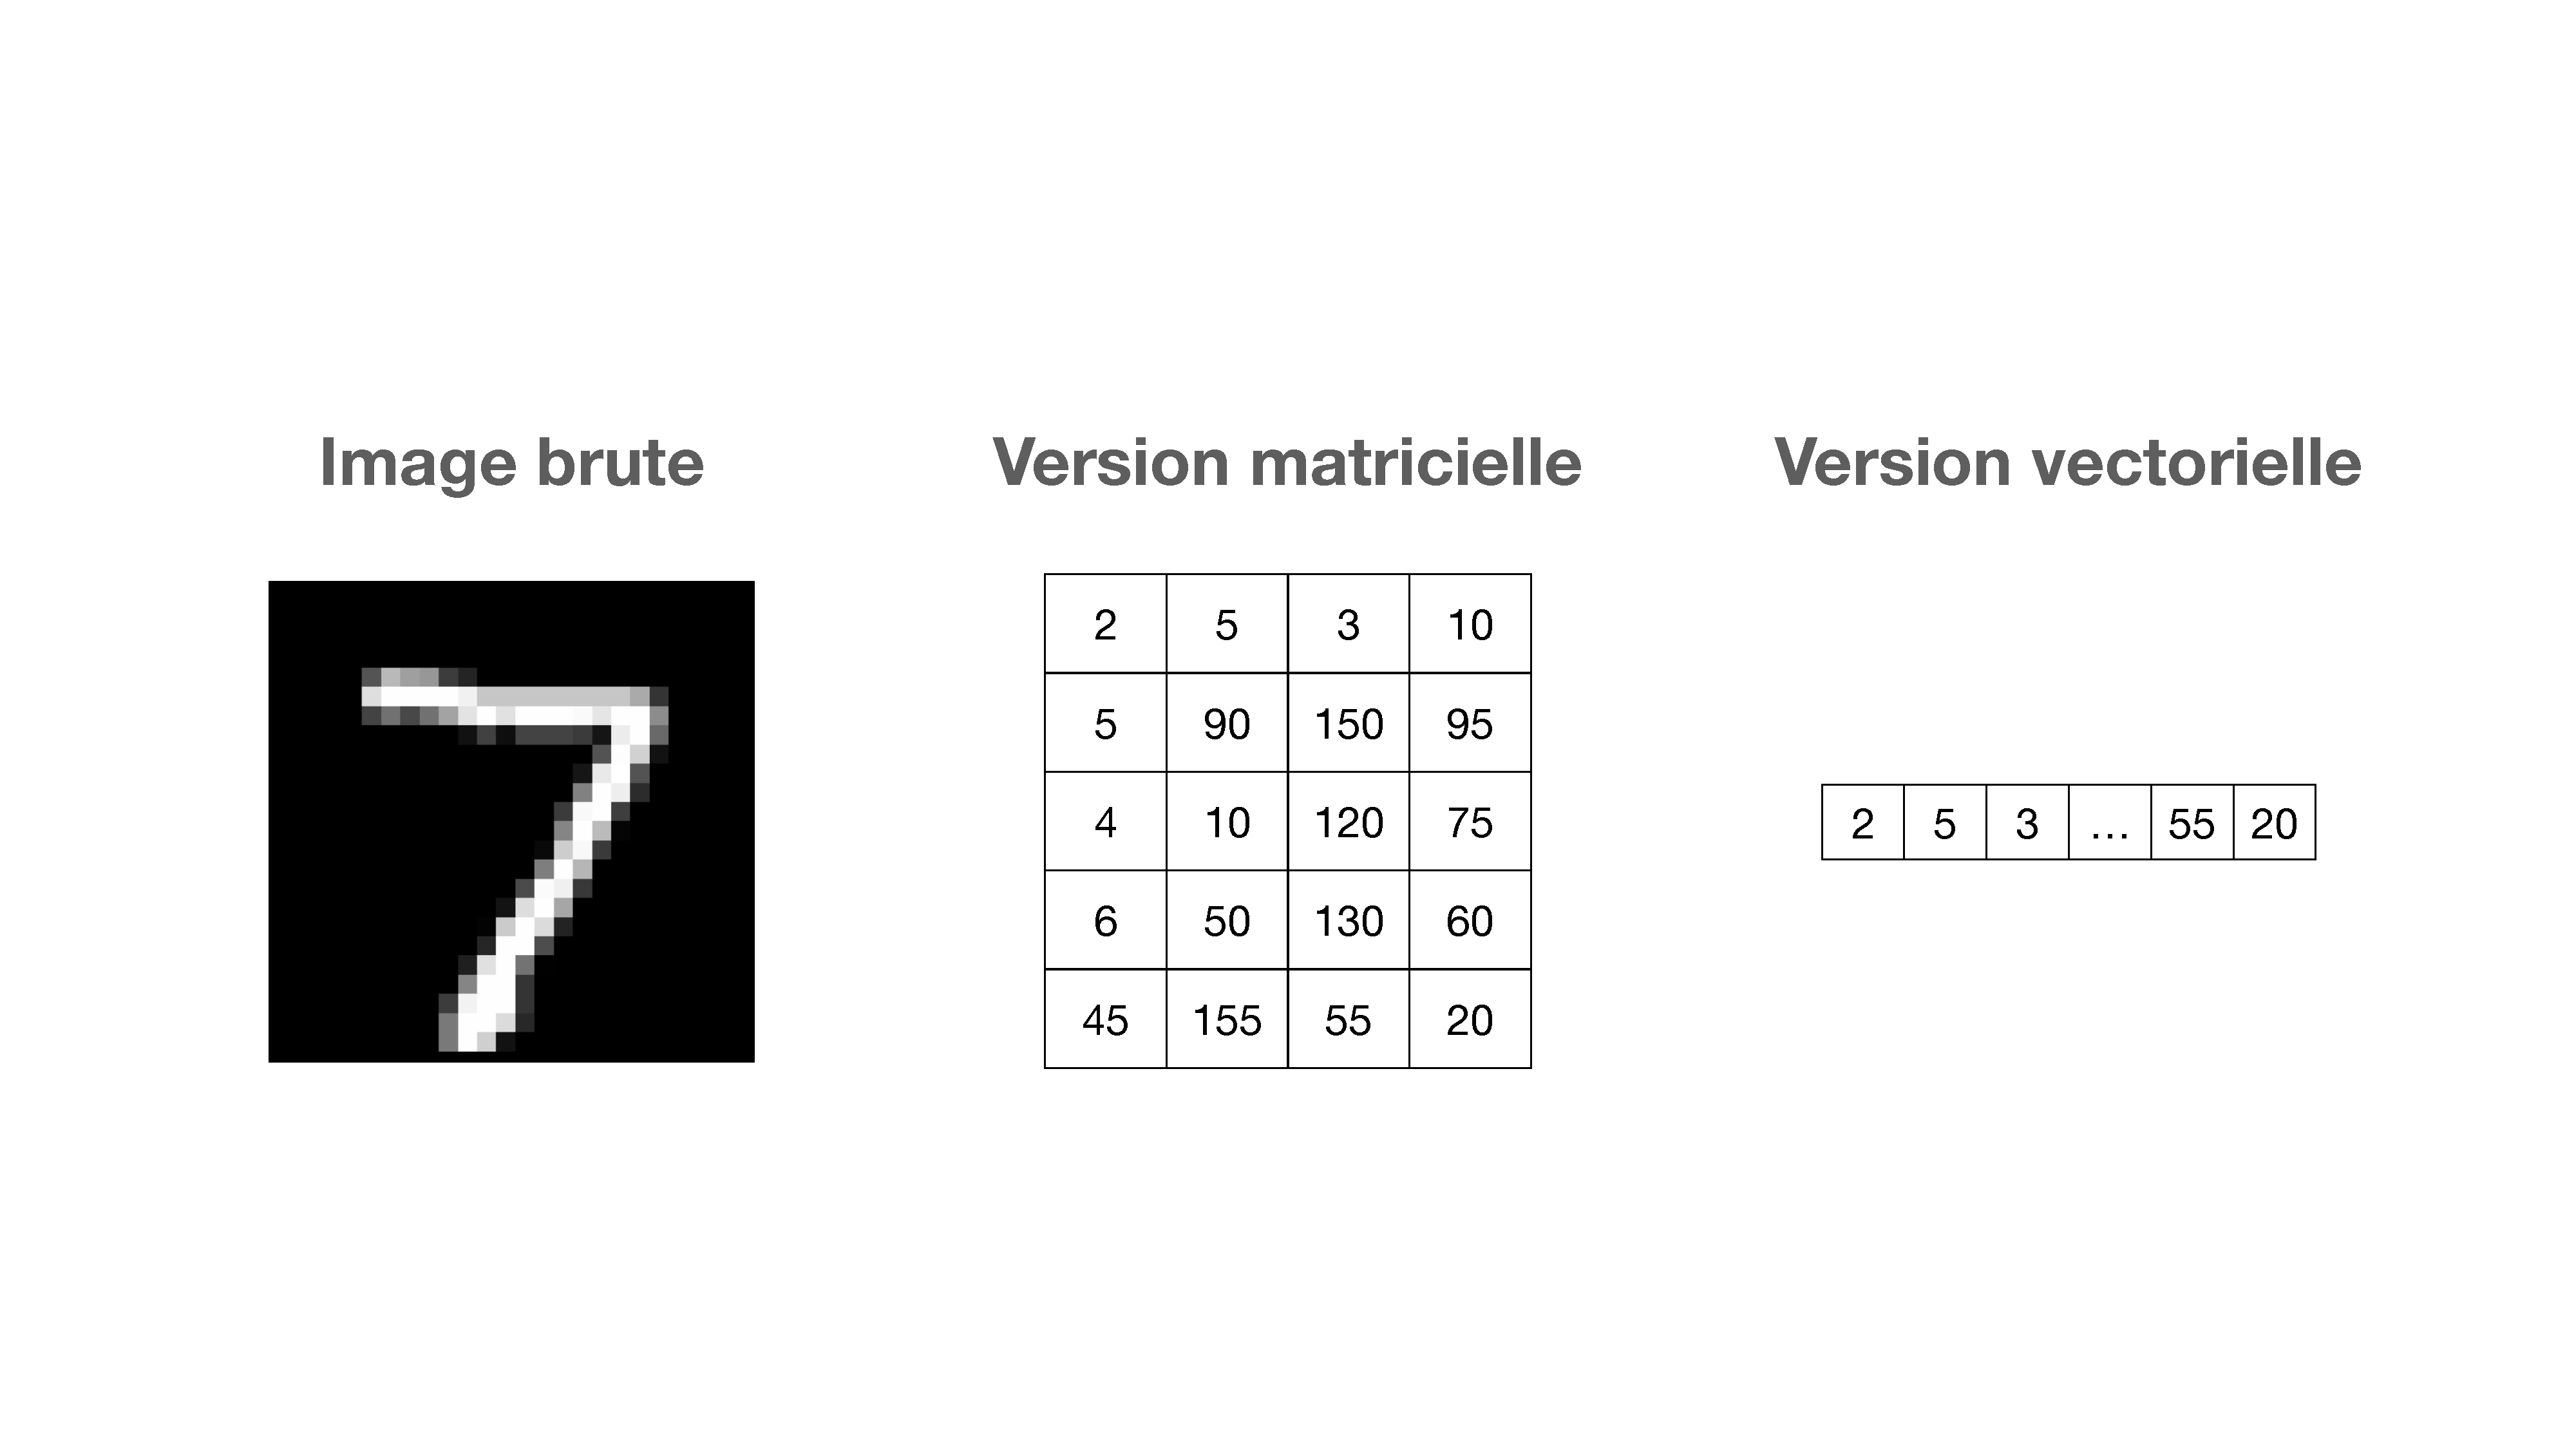
\includegraphics[width=1\linewidth]{images/keynote/one-hot-transfo}
		\caption{Images à un seul canal ("noir et blanc")}
	\end{subfigure}
	\begin{subfigure}{12cm}
		\centering
		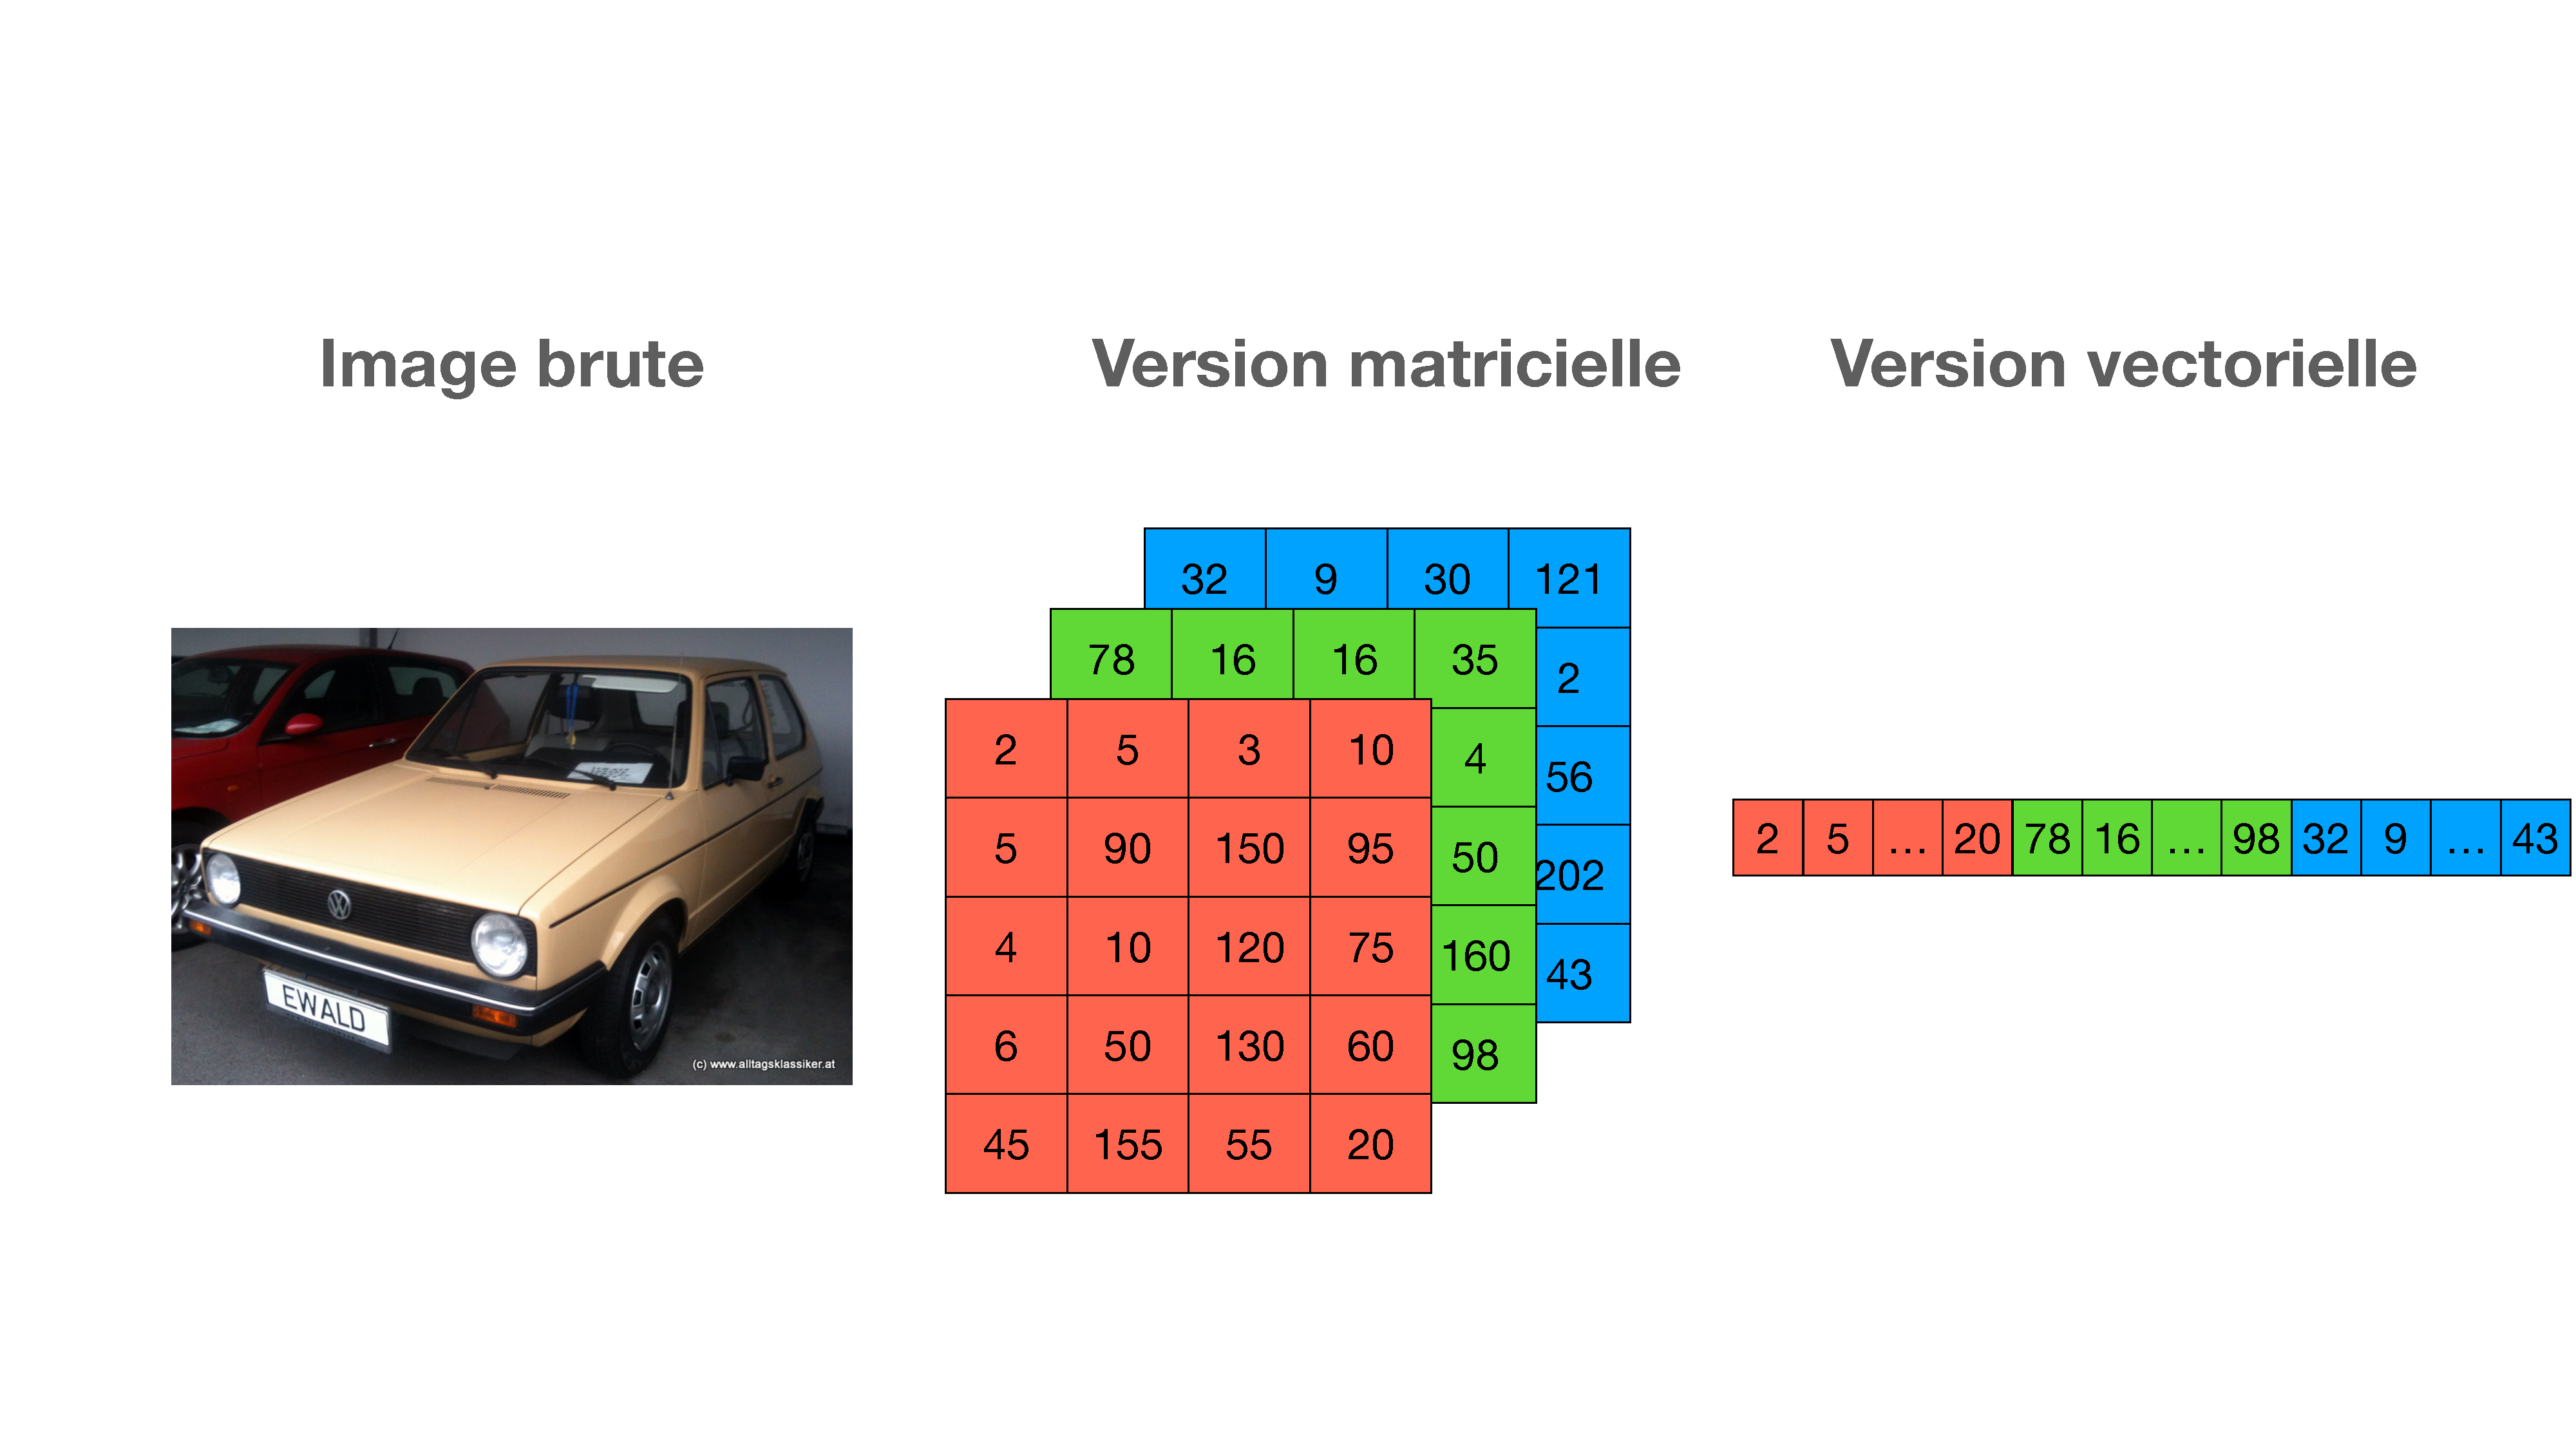
\includegraphics[width=1\linewidth]{images/keynote/one-hot-transfo-rgb}
		\caption{Images à 3 canaux (\textit{RGB})}
	\end{subfigure}
	\caption{Figure illustrant notre méthodologie pour transformer une image d'entrée brute en format vectoriel selon le nombre de canaux de l'image. Les valeurs présentées dans les matrices sont fictives.}
		\label{fig:one_hot}
\end{figure}


Les $n$ observations de notre jeu d'entraînement proviennent d'un mélange à proportion $(1-p)$ d'observations identiquement distribuées dites "normales" et $p$ d'observations identiquement distribuées dites anormales. Pour indiquer si la matrice $\boldsymbol{X^{(i)}}$ provient de la population dite "normale" $\mathcal{N}$, soit $ \boldsymbol{X^{(i)}}\in\mathcal{N}$, on utilise la fonction indicatrice définie ci-dessous,

\begin{gather}  \label{eq:ind_anomaly}
\delta_{i}=
\begin{cases}
0 & \text{si $\boldsymbol{X^{(i)}}\in\mathcal{N}$} \\
1 & \text{si $\boldsymbol{X^{(i)}}\not\in\mathcal{N}$}.
\end{cases}
\end{gather}

On suppose que la proportion $p$ est faible, typiquement moins de 5\%. Dans la pratique, nous ne connaissons pas la valeur des $\delta_i$, ce qui veut dire que nous ne pouvons connaître le pourcentage réel d'anomalies $p$. 

Nous avons également $k$ observations indépendantes de matrices constituées des mêmes $d \times d$ dimensions dans un jeu de données test $\mathcal{X^*} = \{\boldsymbol{X^{*(1)}},...,\boldsymbol{X^{*(k)}}\}$. On suppose que le pourcentage d'anomalies $p^*$ dans ce jeu de données est similaire ou supérieur à $p$. C'est donc dire que parmi ces $k$ observations, $(1-p^*)$ proviennent de la même distribution $\mathcal{N}$ que les données du jeu d'entrainement et $p^*$ sont des anomalies (également de la même population d'anomalies que le jeu d'entrainement). De la même manière que pour le jeu de données d'entraînement $\mathcal{X}$, nous ne savons pas si une matrice $\boldsymbol{X^{*}}$ du jeu de données test provient de la population dite "normale" $\mathcal{N}$. Nous ne connaissons donc pas non plus le pourcentage réel $p^*$. Pour indiquer si la matrice $\boldsymbol{X^{*(i)}}$ provient de la population dite "normale" $\mathcal{N}$, soit $ \boldsymbol{X^{*(i)}}\in\mathcal{N}$, on utilise la même fonction indicatrice que celle définie dans l'équation \ref{eq:ind_anomaly}:

\begin{gather}  \label{eq:ind_anomaly}
\delta^{*}_{i}=
\begin{cases}
0 & \text{si $\boldsymbol{X^{*(i)}}\in\mathcal{N}$} \\
1 & \text{si $\boldsymbol{X^{*(i)}}\not\in\mathcal{N}$}.
\end{cases}
\end{gather}


\section{Description de l'approche}

Notre approche se divise essentiellement en 2 étapes. La première étape implique d'entraîner un autoencodeur variationnel pour apprendre les caractéristiques de la population normale du jeu de données d'entraînement $\mathcal{X}$. La deuxième étape consiste à définir un cadre décisionnel à partir des représentations latentes de l'autoencodeur entraîné nous permettant ainsi d'identifier les anomalies dans le jeu de données de test $\mathcal{X^*}$ avec seuil $\alpha$ similaire à un niveau de confiance, que nous appellerons niveau de filtration.

\subsection{Entraîner l'autoencodeur} \label{meth:train-vae}

La première étape consiste à utiliser le jeu de données d'entraînement $\mathcal{X}$ pour entraîner l'autoencodeur variationnel. Étant donné que $\mathcal{X}$ ne contient presque pas d'anomalies, cela devrait permettre d'appendre les caractéristiques, ou la distribution, de la population dite "normale". Cette distribution apprise sera contenue dans la représentation latente du VAE entraîné, ou plus spécifiquement dans les couches $\mu$ et $\sigma$ du réseau. Ces deux couches précèdent la couche latente et permettent de générer celle-ci de manière stochastique, comme nous l'avons vu dans la section \ref{background-vae}. Les VAE sont généralement entraînés avec une fonction de coût à deux composantes (voir l'équation \ref{eq:loss_vae}). Une de ces deux composantes est associée à la représentation latente du réseau, s'assurant ainsi que celle-ci s'approche d'une distribution a priori, soit une $N(0, I)$ dans notre cas. Pour ce faire, les valeurs des couches $\mu$ et $\sigma$ doivent s'approcher des paramètres de la loi a priori, soit les vecteurs $(\mathbf{0}, \mathbf{1})$ = $(0^m, 1^m)$ dans le cas d'une représentation latente à $m$ dimensions; nous pourrons d'ailleurs tirer avantage de cette hypothèse a priori dans notre règle de décision que nous allons décrire en détails à la prochaine section. La deuxième composante de la fonction de perte, soit l'erreur de reconstruction, demeure primordiale dans l'entraînement du réseau. Dans sa forme la plus simple, cette erreur de reconstruction est définie pixel par pixel. Dans le cas de l'erreur quadratique moyenne, cette composante de perte peut être définie pour la contribution d'une observation $i$ comme

\begin{gather} \label{eq:mse_loss}
L(\boldsymbol{x^{(i)}}, p_\phi\{q_\theta(\boldsymbol{x^{(i)}})\}) = \frac{1}{d^2} \sum_{l=1}^{d^2} (x^{(i)}_{l} - p_\phi\{q_\theta(\boldsymbol{x^{(i)}})\}_l)^2,
\end{gather}

où $p_\phi\{q_\theta(\boldsymbol{x^{(i)}})\}_l$ est le $l$-ème élément du vecteur ou de la matrice de sortie $p_\phi\{q_\theta(\boldsymbol{x^{(i)}})\}$ donnée par l'équation \ref{eq:output}. Dans le cas d'une image, le $l$-ème élément correspond au $l$-ème  pixel de l'image.

La fonction de perte définie à l'équation \ref{eq:mse_loss} accorde autant d'importance à chacun des pixels de l'image. C'est donc dire que le réseau a pour objectif de bien reconstruire autant les pixels en arrière-plan que les pixels centraux. Dans notre cas,  on cherche à trouver des anomalies au niveau du contenu global de l'image. Pour illustrer ce qu'on veut dire par contenu global, la figure \ref{fig:exemple_global} montre quelques exemples d'images considérées comme "normales" et "anormales". Dans la figure \ref{fig:exemple_global}, on peut y voir que les images "normales" de la sous-figure \ref{fig:sfig1} correspondent à des voitures dans un environnement extérieur. La sous-figure \ref{fig:sfig2} présente des images "anormales", où on peut y apercevoir des chiens dans un environnement extérieur. Même si l'arrière-plan de ces images est similaire à celui de \ref{fig:sfig1}, le contenu global correspond à des images de chiens et non de voiture. À l'opposé, on peut apercevoir à la sous-figure \ref{fig:sfig3} des images de voitures correspondant à des modèles particuliers, des environnements intérieurs et aussi contenant des écritures sur les marges supérieures et inférieures de l'image. Malgré ces observations, le contenu global de ces images correspond tout de même à des voitures, ce qui nous amène à les considérer comme des images dites "normales".

\begin{figure} [htb]
	\begin{subfigure}{.33\textwidth}
		\centering
		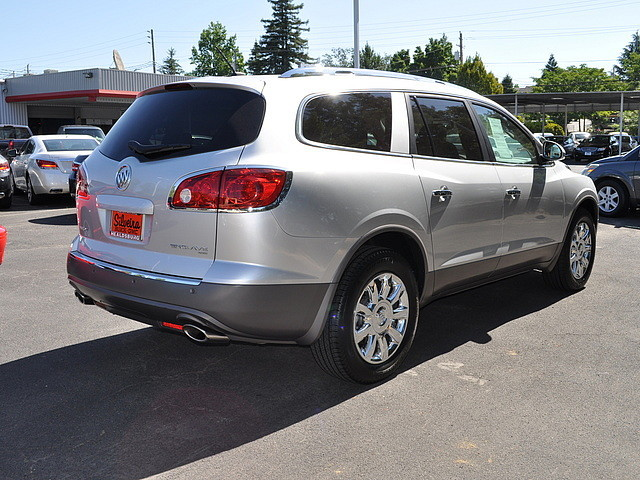
\includegraphics[width=.8\linewidth,height=3cm]{images/images_anomalies/inlier-1}
		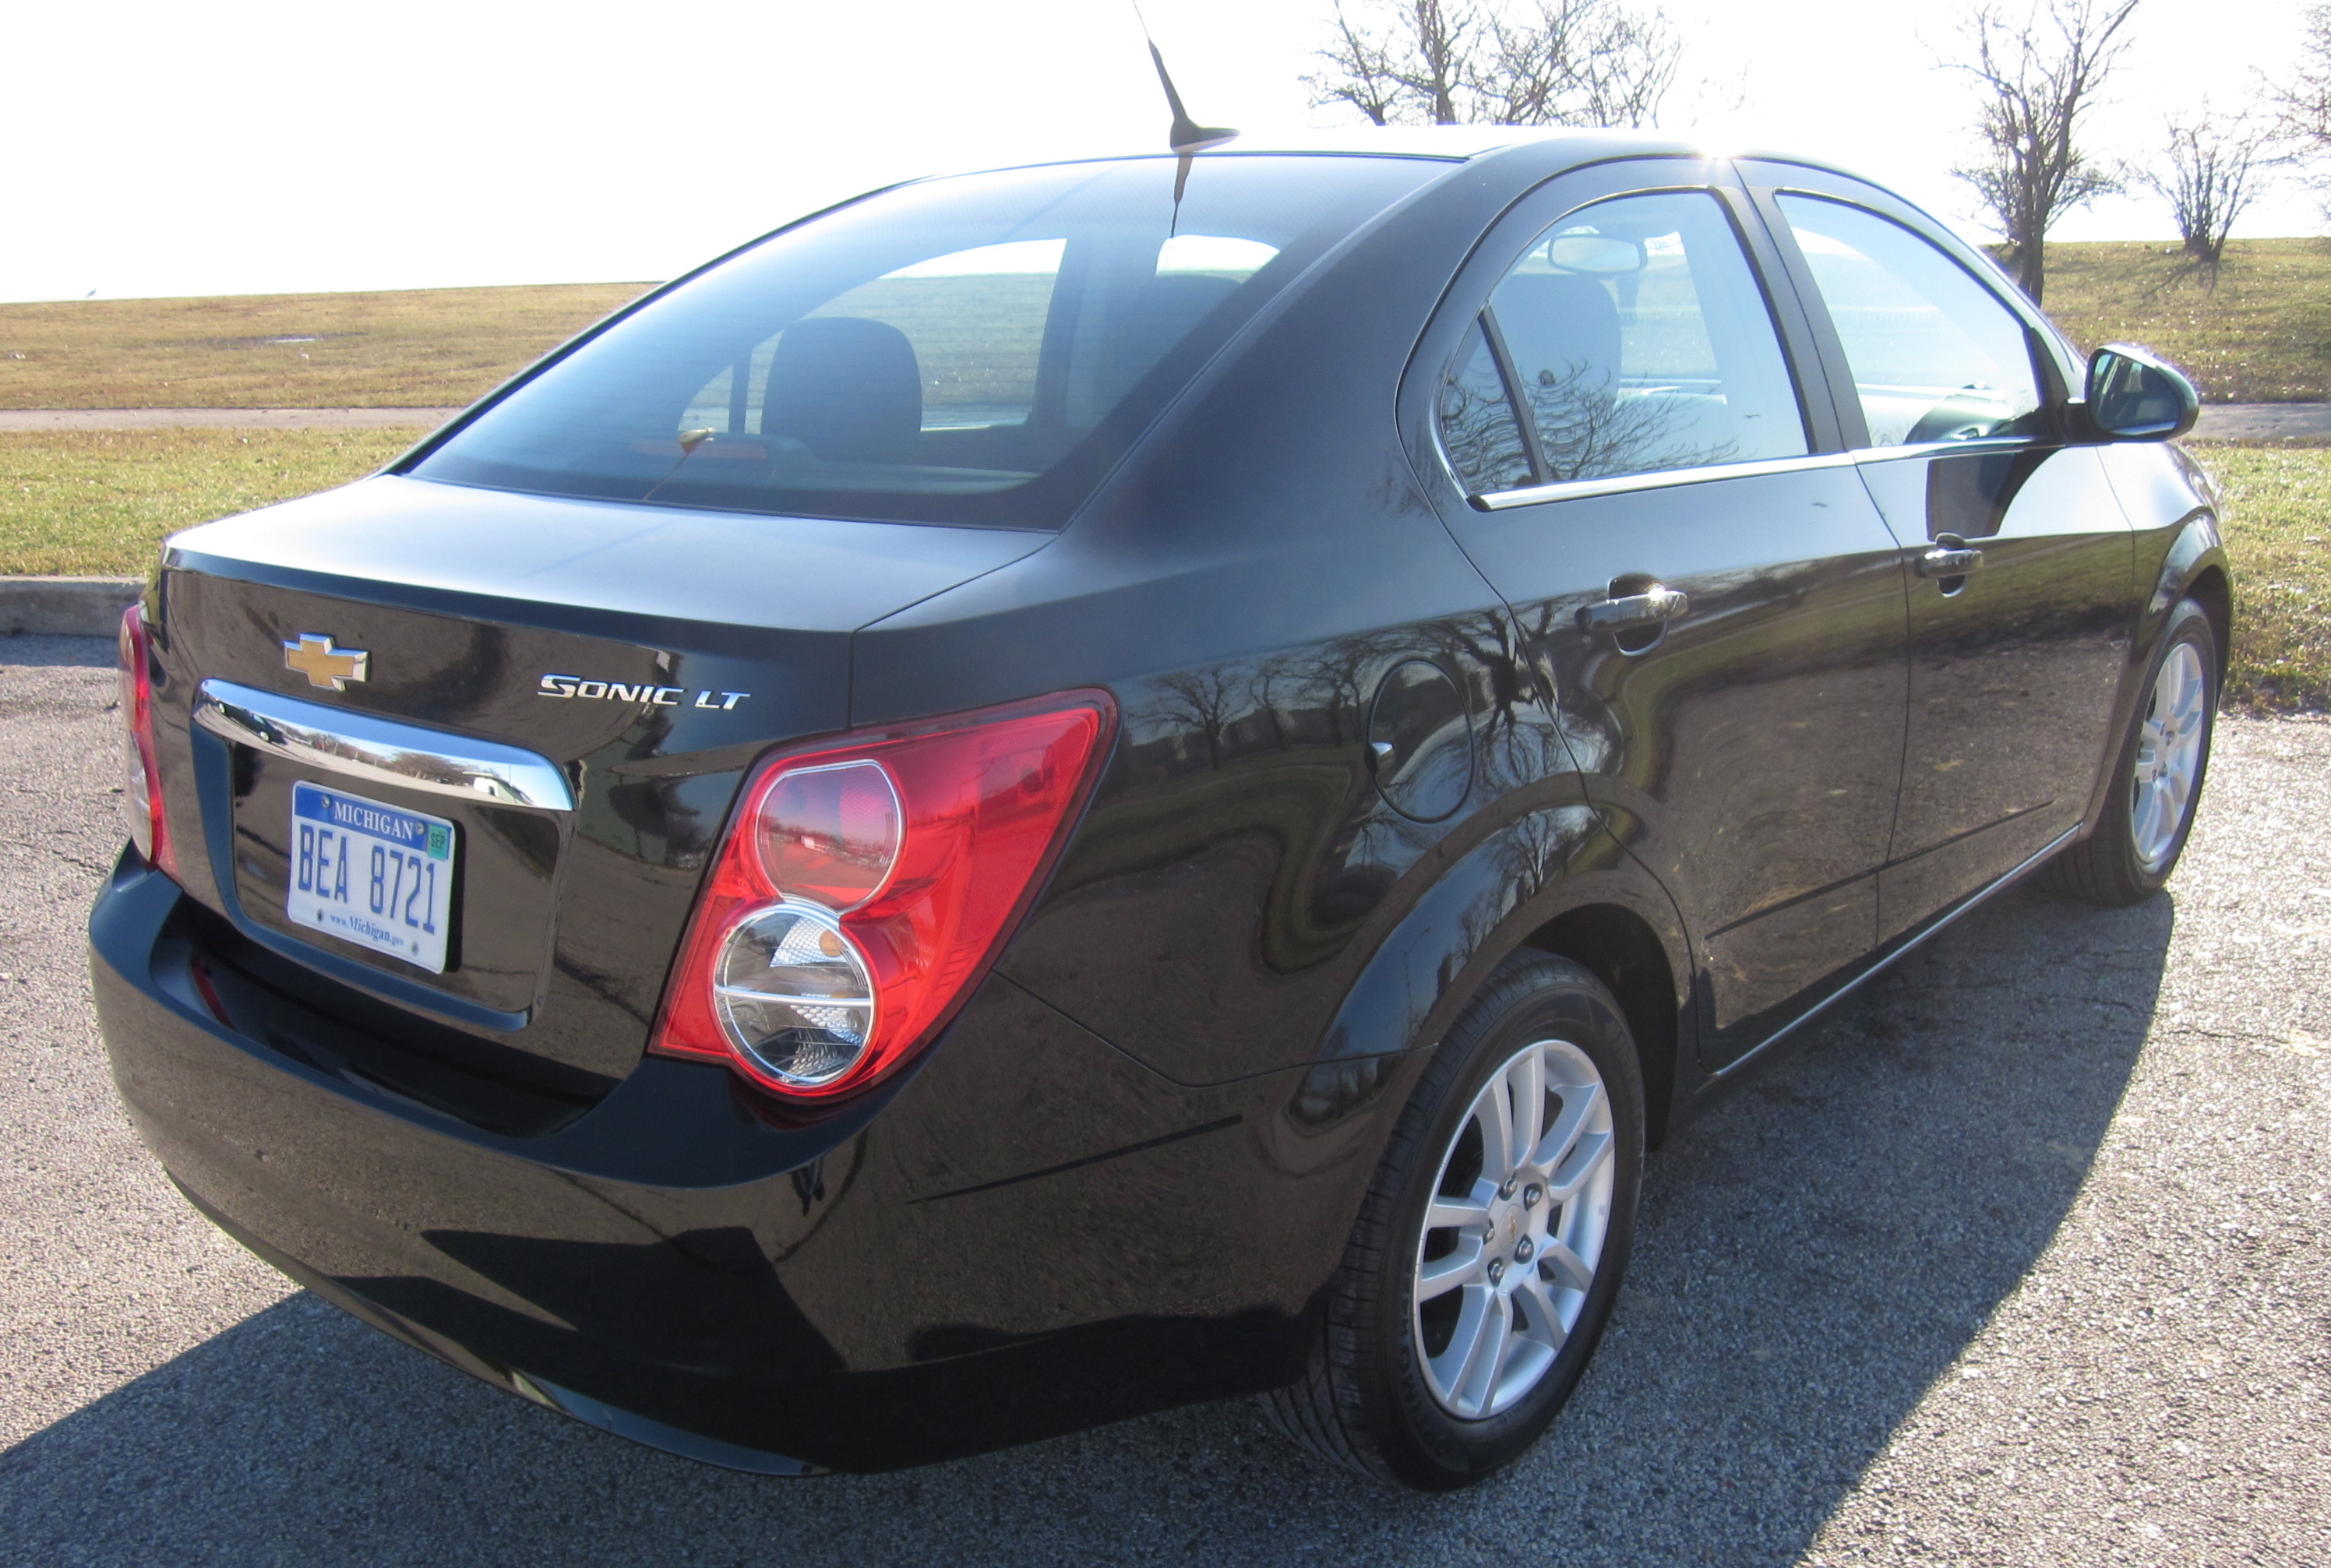
\includegraphics[width=.8\linewidth,height=3cm]{images/images_anomalies/inlier-2}
		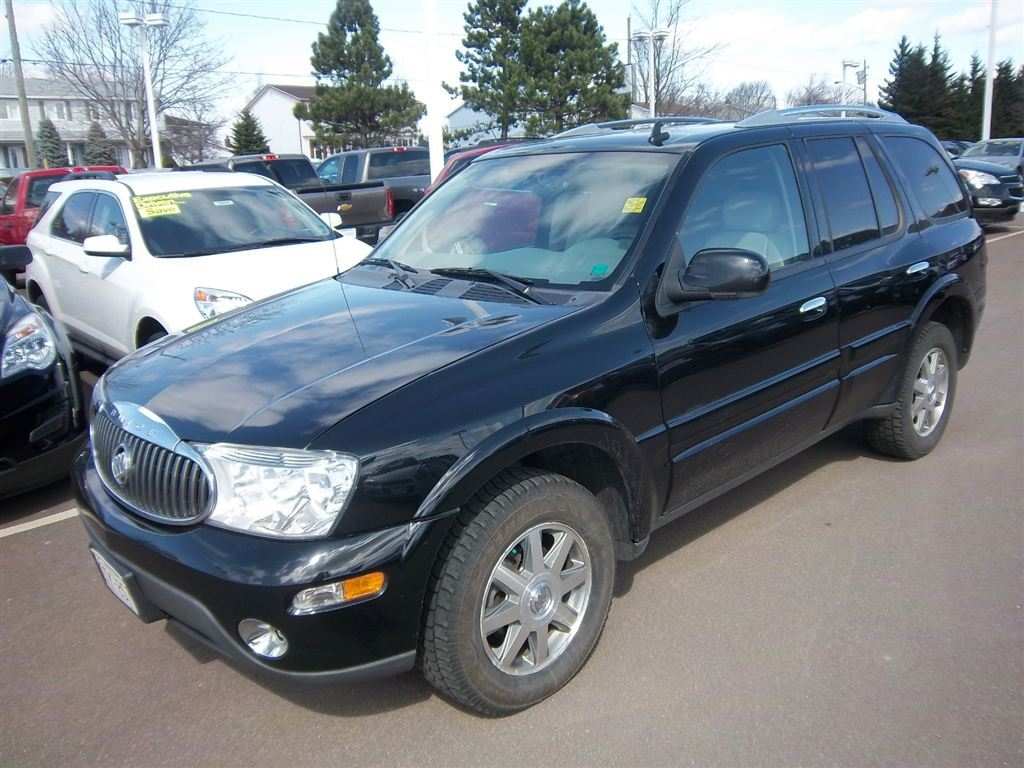
\includegraphics[width=.8\linewidth,height=3cm]{images/images_anomalies/inlier-3}
		\caption{Images "normales"}
		\label{fig:sfig1}
	\end{subfigure}%
	\begin{subfigure}{.33\textwidth}
		\centering
		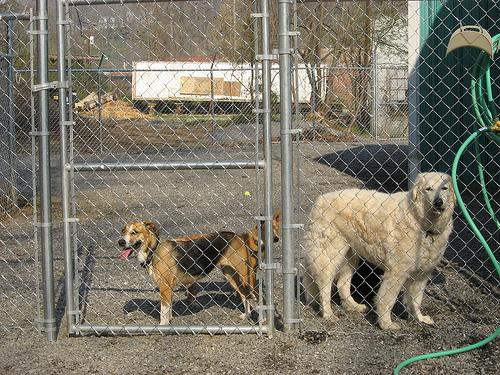
\includegraphics[width=.8\linewidth,height=3cm]{images/images_anomalies/anomalie-1}
		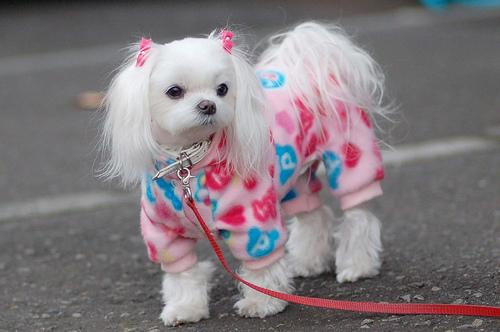
\includegraphics[width=.8\linewidth,height=3cm]{images/images_anomalies/anomalie-2}
		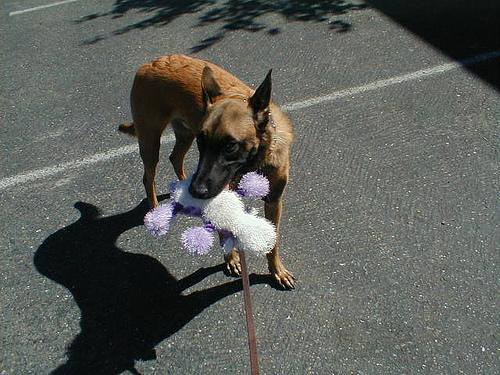
\includegraphics[width=.8\linewidth,height=3cm]{images/images_anomalies/anomalie-3}
		\caption{Images "anormales"}
		\label{fig:sfig2}
	\end{subfigure}
	\begin{subfigure}{.33\textwidth}
		\centering
		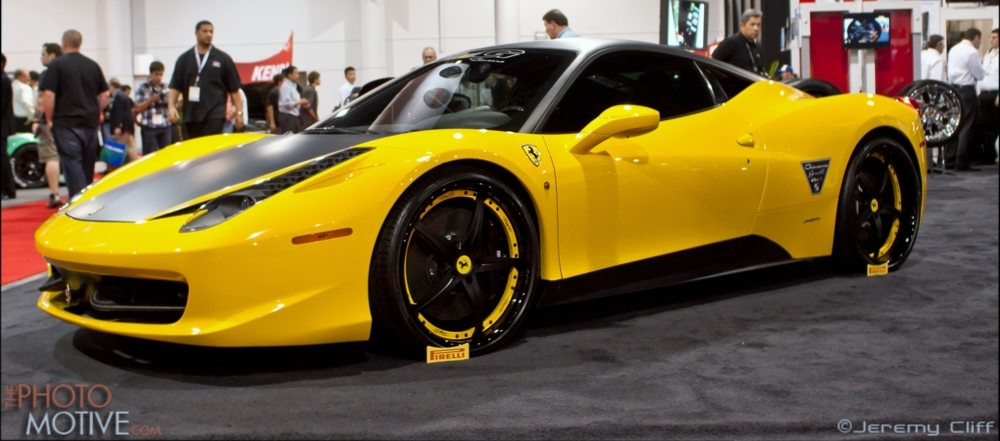
\includegraphics[width=.8\linewidth,height=3cm]{images/images_anomalies/inlier-4}
		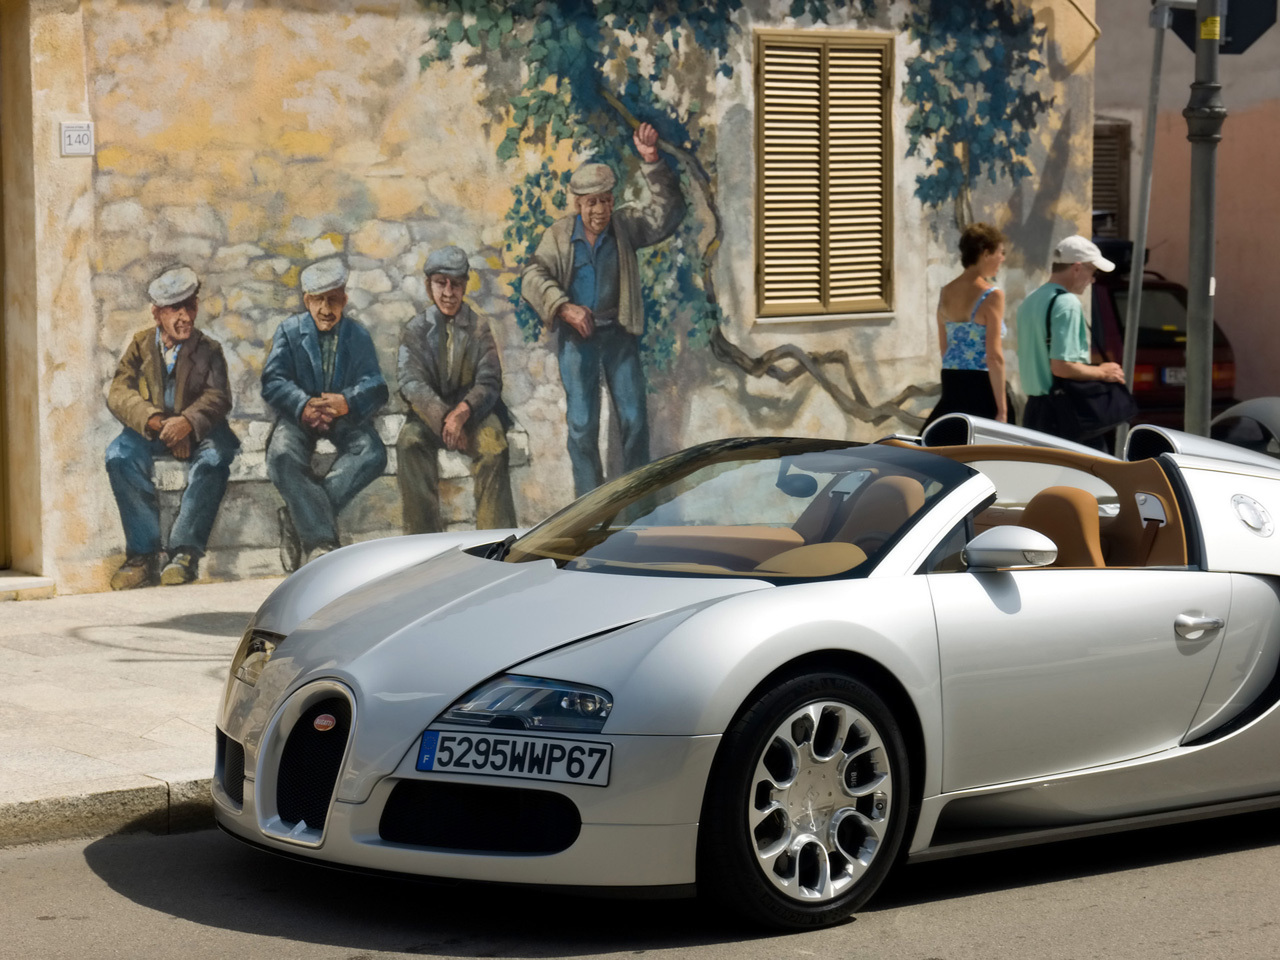
\includegraphics[width=.8\linewidth,height=3cm]{images/images_anomalies/inlier-5}
		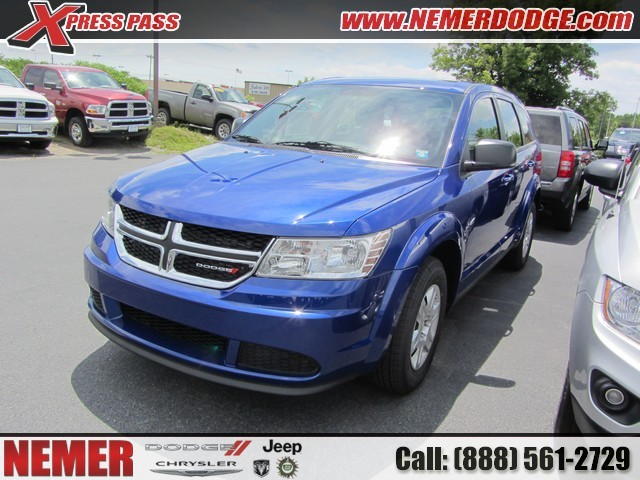
\includegraphics[width=.8\linewidth,height=3cm]{images/images_anomalies/inlier-6}
		\caption{Images "normales"}
		\label{fig:sfig3}
	\end{subfigure}
	\centering
	\caption{Figure illustrant des exemples d'images considérées comme "normales" et d'autres comme "anormales". Dans ce cas, les images dites "normales" sont des images de voitures.}
	\label{fig:exemple_global}
\end{figure}

 La figure \ref{fig:exemple_global} illustre le fait qu'il devient pertinent de trouver une manière d'accorder plus d'importance au contenu global de l'image. Pour ce faire, on utilise un concept qui s'appelle \textit{perceptual loss}. Dans ce type d'optimisation, on calcule la perte en se basant sur une couche spécifique d'un autre réseau de neurones pré-entraîné sur beaucoup plus d'images. En pratique, on utilise généralement des architectures de réseaux connus,  comme \textit{VGG} \citep{DBLP:journals/corr/SimonyanZ14a}  ou \textit{ResNet} \citep{DBLP:journals/corr/HeZRS15}, pré-entraînés sur \textit{ImageNet} \citep{deng2009imagenet}. Cette approche est d'ailleurs utilisée pour transformer le style d'une image, par exemple pour donner le style d'un peintre célèbre à une image quelconque \citep{Johnson2016Perceptual}. La figure \ref{fig:perceptual} illustre le mécanisme exact du calcul de la perte. On peut y voir que l'erreur de reconstruction du réseau n'est plus calculée directement entre la sortie du réseau $\hat{x}$ et l'entrée $x$. En effet, les deux composantes sont plutôt données en entrée à un autre réseau, et l'erreur est calculée en comparant plutôt une représentation précise de ce réseau obtenue par ces 2 composantes.

\begin{figure}[h]
	\centering
	\begin{tikzpicture}[shorten >=1pt,draw=black!50, node distance=\layersep, square/.style={regular polygon,regular polygon sides=4}]
	\tikzstyle{neuron}=[circle,fill=black!25,minimum size=30pt,inner sep=0pt]
	\tikzstyle{network}=[square,fill=black!25,minimum size=75pt,inner sep=0pt]
	\tikzstyle{input neuron}=[neuron, fill=green!50];
	\tikzstyle{graph}=[network, fill=white, draw=black];
	\tikzstyle{hidden neuron}=[neuron, fill=blue!50];
	\tikzstyle{annot} = [text width=4em, text centered]
	
	% Draw input (x)
	\node[input neuron] (input) at (0,-5) {$\boldsymbol{x}$};
	
	% Draw the VAE 
	\node[graph] (vae) at (3,-2.5) {$p_{\phi}\{q_{\theta}(\boldsymbol{x})\}$};
	
	% Draw the output (\hat(x)) with x below
	\node[hidden neuron] (x_chap) at (6,-2.5) {$\hat{\boldsymbol{x}}$};
	%\node[input neuron] (input-2) at (6,-5) {$\boldsymbol{x}$};
	
	% Draw the VGG16
	\node[graph] (vgg16_1) at (9,-2.5) {$g(\cdot)$};
	\node[graph] (vgg16_2) at (9,-5) {$g(\cdot)$};
	
	
	% Draw the outputs
	\node[hidden neuron] (input_sortie) at (12,-2.5) {$g(\hat{\boldsymbol{x}})$};
	\node[input neuron] (x_chap_sortie) at (12,-5) {$g(\boldsymbol{x})$};
	
	% Draw arrows
	\path[->, line width=1mm] (input) edge (vae);
	\path[->, line width=1mm] (vae) edge (x_chap);
	\path[->, line width=1mm] (input) edge (vgg16_2);
	\path[->, line width=1mm] (x_chap) edge (vgg16_1);
	\path[->, line width=1mm] (vgg16_1) edge (input_sortie);
	\path[->, line width=1mm] (vgg16_2) edge (x_chap_sortie);
	
	% Annotate the steps
	\node[annot,above of=input, node distance=4.5cm] (h1) {Image d'entrée};
	\node[annot,above of=vae, node distance=2cm] (h2) {VAE};
	\node[annot,above of=vgg16_1, node distance=2cm] (h3) {VGG16*};
	\end{tikzpicture}
	\caption{Figure montrant le mécanisme derrière le concept de \textit{perceptual optimization}. Au lieu de calculer la perte entre $\boldsymbol{x}$ et $\hat{\boldsymbol{x}}$, la perte est calculée entre $g(\boldsymbol{x})$ et $g(\hat{\boldsymbol{x}})$. La fonction $g(a)$ permet d'extraire les valeurs d'une couche spécifique d'un autre réseau pré-entraîné, comme par exemple \textit{VGG16} pré-entraîné sur \textit{ImageNet}.}
	\label{fig:perceptual}
\end{figure}

Étant donné que le réseau correspondant à la fonction $g(a)$ dans la figure \ref{fig:perceptual} est pré-entraîné sur plusieurs images réelles, cela nous permet d'extraire une couche qui contient de l'information à plus bas niveau comme la reconnaissance de lignes, des formes précises, des couleurs, etc. Plus la couche sélectionnée est près de l'entrée du réseau, plus l'information utilisée pour calculer la perte sera simple et brute. À l'inverse, si on sélectionne une couche plus près de la sortie, nous serons en mesure de prendre en compte de l'information plus complexe, par exemples des formes particulières \citep{Johnson2016Perceptual}. L'erreur de reconstruction qui était définie à l'équation \ref{eq:mse_loss}, peut maintenant se définir comme suit:

\begin{gather} \label{eq:perceptual_loss}
L(\boldsymbol{x}^{(i)}, p_\phi\{q_\theta(\boldsymbol{x}^{(i)})\}) = \frac{1}{d^2} \sum_{l=1}^{d^2} \Big[g(x^{(i)})_{l} - g(p_\phi\{q_\theta(\boldsymbol{x}^{(i)})\})_{l}\Big]^2.
\end{gather}

L'objectif d'utiliser ce type de perte est d'optimiser la reconstruction du réseau non pas sur les valeurs précises des pixels reconstruites en sortie, mais plutôt sur des représentations contenant de l'information plus structurée. Cela permet entre autres d'orienter l'apprentissage vers la reconstruction du contenu à plus haut-niveau, plutôt que sur la reconstruction parfaite de chaque pixel. Il est important de rappeler que notre objectif est de trouver des anomalies, et non reconstruire parfaitement des images.

Une fois l'autoencodeur variationnel entraîné, c'est-à-dire lorsque les paramètres $\theta$ et $\phi$ sont fixés, il nous est donc possible d'utiliser la partie encodeur du réseau, $q_{\theta}(\cdot) $, pour transformer les images, ou les données en entrée, en une paire de vecteurs $(\boldsymbol{\mu}, \boldsymbol{\sigma})$:

\begin{gather}  \label{eq:encodeur}
q_{\theta}(\boldsymbol{x}) = (\boldsymbol{\mu}, \boldsymbol{\sigma}), \qquad \boldsymbol{\mu} \in \mathbb{R}^m, \boldsymbol{\sigma} \in \mathbb{R}^m.
\end{gather}

Certains détails supplémentaires concernant l'entraînement de l'autoencodeur variationnel seront décrits dans la section \ref{DA_VAE}.


\subsection{Définir le cadre décisionnel} \label{cadre_decisionnel}

La prochaine étape de notre approche consiste à définir un cadre décisionnel nous permettant de discriminer les anomalies des observations "normales". Avec ce cadre décisionnel, on cherche à savoir si une observation provenant du jeu de données test, soit $\boldsymbol{X}^{*}$, provient de la population normale $\mathcal{N}$. Pour ce faire, nous allons définir une métrique ou une statistique de distance, obtenue via une fonction $T(\cdot)$, que nous pourrons ensuite comparer à un seuil de décision $s$. La valeur de la statistique de distance et le seuil nous permettront de définir une région $R_{N}=\{x :T(x)<s\}$ ou $R_{N}=\{x :T(x)>s\}$, pour un $s>0$. Si une observation $\boldsymbol{x^{(i)}}$ se retrouve dans cette région $R_{N}$, nous pourrons supposer que celle-ci est de la population $\mathcal{N}$, donc poser $\delta^{*}_{i}=0$. Afin de prendre en compte l'apprentissage fait par l'autoencodeur variationnel, la statistique de distance sera plutôt basée sur la représentation latente obtenue par l'encodeur $q_\theta(\cdot)$ pour une observation $\boldsymbol{x^{(i)}}$. Cela nous permet de réécrire la région $R_N$:

\begin{gather}  \label{eq:region}
R_{N}=\{x :T(q_\theta(\boldsymbol{x^{(i)}}))<s\}.
\end{gather}

Pour obtenir cette région $R_N$, il faut donc procéder en 2 étapes. La première consiste à calculer la statistique de distance, donnée par la fonction $T(\cdot)$, sur chacune des instances de notre jeu de données d'entraînement. La deuxième étape consiste à calculer le seuil $s$ avec l'aide d'un niveau de filtration $\alpha$ similaire à un niveau de confiance. Ces deux étapes nous permettront de définir notre région de décision nous permettant d'inférer quelles observations du jeu de données test devraient être étiquetées comme des anomalies. Les prochaines sections décrivent plus en détails comment calculer les statistiques de distance et comment définir le seuil à partir de celles-ci.

\subsubsection{Définir une statistique de distance}

 À partir de la section \ref{meth:train-vae}, nous sommes en mesure d'obtenir des représentations latentes, encodées sous forme de vecteurs, pour chaque instance de notre jeu de données $\mathcal{X}$. Nous allons utiliser ces représentations latentes pour générer une statistique de distance selon laquelle nous prévoyons un comportement différent selon si une observation est "normale" ou "anormale". La métrique que nous avons choisie pour définir notre statistique de distance est la distance de Kullbach-Leibler entre une loi $N(\boldsymbol{\mu}, \boldsymbol{\sigma})$ et une loi $N(0,I)$, où les vecteurs $(\boldsymbol{\mu}, \boldsymbol{\sigma})$ correspondent à la représentation latente obtenue par l'autoencodeur variationnel. Cette statistique de distance, que nous appellerons $T$, est donc définie comme suit pour une observation $i$:
 
 \begin{gather}  \label{eq:metrique}
 T^{(i)} = D_{KL}\big[N(\boldsymbol{\mu^{(i)}}, \boldsymbol{\sigma^{(i)}}) || N(0, I)\big].
 \end{gather}
 
 La statistique de distance $T$ nous permet donc de quantifier la distance entre les vecteurs $(\boldsymbol{\mu}, \boldsymbol{\sigma})$ de la représentation latente d'une observation $i$ et les vecteurs $(\boldsymbol{0_m}, \boldsymbol{1_m})$ correspondant aux paramètres d'une loi $N(0,I)$. Nous pouvons donc calculer cette distance pour chacune des $n$ observations du jeu de données d'entraînement $\mathcal{X}$ pour obtenir l'ensemble de valeurs $T_{\mathcal{X}}=\{T^{(1)}, ..., T^{(n)}\}$. Le raisonnement derrière le choix de cette métrique réside dans le fait que celle-ci est utilisée comme composante dans le critère de perte utilisé lors de l'entraînement de l'autoencodeur. Si l'importance relative de cette composante de perte est différente entre les anomalies et les observations "normales", cette différence devrait se refléter dans les représentations latentes, donc aussi dans la statistique de distance calculée. Le débalancement naturel des anomalies dans un jeu de données nous amène à faire l'hypothèse que les deux composantes de perte ne seront pas optimisées de manière similaire entre les anomalies et les observations "normales".
 
 Maintenant que nous avons fait l'hypothèse que les valeurs des statistiques de distance des anomalies différeront des valeurs des statistiques de distance des observations "normales", il reste à savoir si une valeur élevée est un signe d'anomalie ou l'inverse. Pour savoir comment interpréter la valeur de la statistique, il faut inspecter certaines observations du jeu de données d'entraînement. Nous proposons d'analyser certaines observations ayant des statistiques de distance élevées et certaines observations ayant des statistiques de distance faibles. En analysant les deux extrémités, nous serons en mesure de conclure comment les représentations latentes des observations dites "normales" se comportent par rapport à la loi $N(0,I)$. Nos expérimentations révèlent 2 scénarios possibles par rapport au comportement des représentations latentes observations "normales" par rapport à la $N(0,I)$:

\begin{enumerate} \label{liste_scenarios}
	\item \textbf{Près de la $N(0,I)$:} Les valeurs des statistiques de distance correspondant aux observations "normales" sont faibles dans l'ensemble $T_{\mathcal{X}}$.
	\item \textbf{Éloigné de la $N(0,I)$:} Les valeurs des statistiques de distance correspondant aux observations "normales" sont élevées dans l'ensemble $T_{\mathcal{X}}$.
\end{enumerate}

Les deux scénarios décrits ci-dessus sont illustrés en exemple dans la figure \ref{fig:scenarios}. Dans cette figure, on peut voir le paramètre $\mu$ sur l'axe des $x$ et le paramètre $\sigma^2$ sur l'axe des $y$, ce qui représenterait le cas où les représentations latentes auraient 1 seule dimension, soit une valeur générée par une loi $N(\mu, \sigma^2)$. On peut y voir la différence par rapport au point central (les 2 croix noires) entre les observations connues "normales" (les points rouges) et les observations connues "anormales" (les points bleus).  La croix en forme de "+" correspond au point central des observations "normales" et la croix en forme de "x" correspond au point central des observations "anormales". Cette figure illustre le cas où l'on connait l'étiquette de tous les observations. Dans un cas réel, nous ne connaitrons pas ces étiquettes, il faudra donc tenter de déterminer lequel de ces 2 scénarios semble le plus plausible en analysant certaines observations étant très près et très éloignés du point central $(\boldsymbol{0_m}, \boldsymbol{1_m})$.

\begin{figure} [h]
	\centering
	\begin{subfigure}{6cm}
		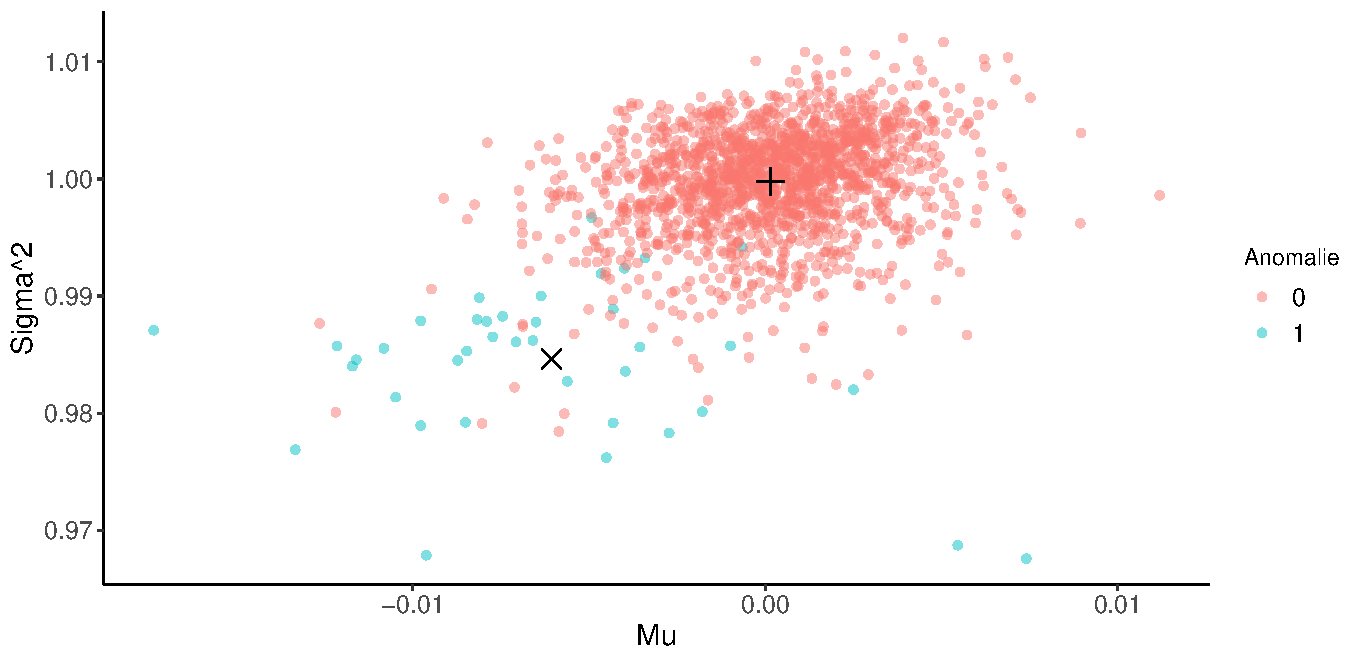
\includegraphics[width=6cm]{images/plot_near.pdf}
		\caption{Scénario 1}
	\end{subfigure}
	\begin{subfigure}{6cm}
		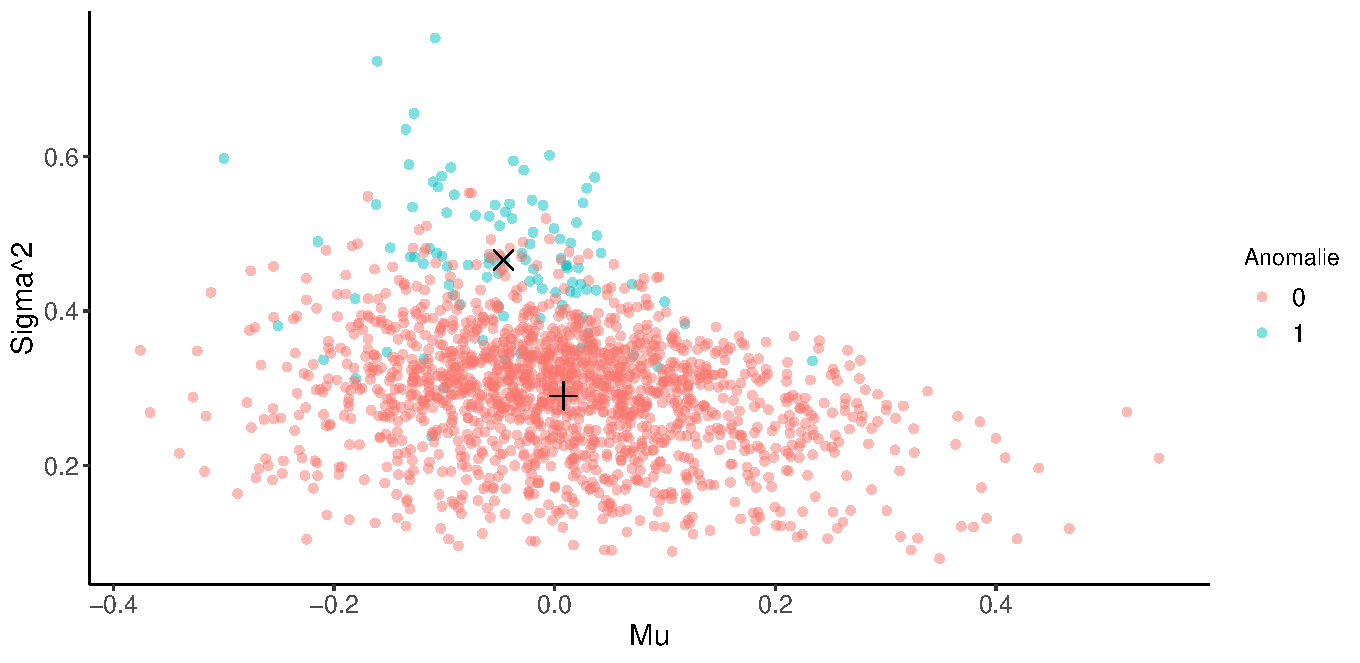
\includegraphics[width=6cm]{images/plot_away.pdf}
		\caption{Scénario 2}
	\end{subfigure}
	\caption{Exemples de situations représentant les 2 différents scénarios se rapportant  aux représentation latentes des observations "normales" et "anormales".}
	\label{fig:scenarios}
\end{figure}

Une fois que nous avons défini et analysé les statistiques de distance obtenues sur l'ensemble d'entraînement, nous pouvons passer à la prochaine étape qui consiste à trouver le seuil $s$ nous permettant de définir la région de décision $R_N$.

\subsubsection{Trouver le seuil $s$}

 Pour trouver le seuil $s$, on veut partir d'un niveau de filtration $\alpha$ similaire à un niveau de confiance. Ce niveau de filtration $\alpha$ nous permettra de faciliter la détermination du seuil $s$. Le seuil déterminé avec un niveau de filtration $\alpha$ sera appelé $s_{(1-\alpha)}$. Par exemple, avec un niveau de filtration $\alpha=0.05$, notre seuil $s$ nous permettra d'identifier les observations ayant des statistiques de distances se retrouvant dans les $95\%$ plus "normales" de l'ensemble d'entraînement $\mathcal{X}$. En faisant varier ce paramètre $\alpha$, nous pourrons identifier plus ou moins d'anomalies. 

Pour fixer la exacte du  seuil $s_{(1-\alpha)}$, nous allons extraire une valeur de notre ensemble de statistiques de distance $T_{\mathcal{X}}$. Nous pourrons ensuite comparer cette valeur $s_{(1-\alpha)}$ à la valeur d'une statistique de distance  correspondant à une nouvelle observation pour conclure si cette nouvelle observation fait partie de la région $R_N$. Le scénario identifié à la section précédente nous est nécessaire pour trouver la valeur du seuil $s_{(1-\alpha)}$. Dans le scénario où les observations "normales" sont près de la $N(0,I)$, soit le scénario 1, nous allons préalablement ordonner les valeurs de $T_{\mathcal{X}}$ en ordre croissant. Dans le scénario inverse où les observations "normales" sont éloignées de la $N(0,I)$, soit le scénario 2, nous allons plutôt ordonner les valeurs de $T_{\mathcal{X}}$ en ordre décroissant. Nous définissons $T^{'}_{\mathcal{X}}$, l'ensemble $T_{\mathcal{X}}$ ordonné selon le scénario en question. Le seuil $s_{(1-\alpha)}$ correspond donc à la valeur associée au rang $\lfloor(1 - \alpha) \times n\rfloor$ de l'ensemble $T^{'}_{\mathcal{X}}$:

\begin{gather} \label{eq:seuil}
s_{(1 - \alpha)} = T^{'}_{\mathcal{X} \{(1 - \alpha) \times n\}},
\end{gather}

où $T^{'}_{\mathcal{X} \{(1 - \alpha) \times n\}}$ est la valeur correspondant au rang $\lfloor(1 - \alpha) \times n\rfloor$ de l'ensemble $T^{'}_{\mathcal{X}}$. Ce seuil nous permet de définir la région $R_N$, qui représente la région où une observation est considérée comme "normale". Si on définit $t$ comme étant la valeur d'une statistique de distance calculée comme $t = T(q_\theta(\boldsymbol{x}))$, la région $R_N$ est donnée par:

\begin{gather} \label{eq:region}
	R_{N} = 
	\begin{cases} 
		\big\{t \in \mathbb{R}: t < s_{(1 - \alpha)} \big\} & \text{si les observations "normales" sont près de $N(0, I)$} \\
		\big\{t \in \mathbb{R}: t > s_{(1 - \alpha)} \big\} & \text{si les observations "normales" sont éloignées de $N(0, I)$} 
	\end{cases}
\end{gather}

Pour tester les observations de notre jeu de données test, nous allons calculer les statistiques de distance $T$ des $k$ observations de ce jeu de données $\mathcal{X^*}$. Si la valeur de la statistique de distance $T^{(j)}$ correspondant à l'observation $\boldsymbol{x^{*(j)}}$ fait partie de la région $R_N$, on peut donc conclure que l'observation fait partie de l'ensemble $(1-\alpha)$-normal. Si la statistique de distance $T^{(j)}$ ne fait pas partie de la région $R_N$, on l'étiquettera comme une anomalie.

La région $R_N$ nous permet de définir si une observation est une $\alpha$-anomalie ou non. De manière similaire, on peut également utiliser l'ensemble $T_{\mathcal{X}}$ pour établir un score d'anomalie pour une observation donnée. Ce score d'anomalie est défini entre $[0,1]$, où une anomalie évidente devrait avoir un score se rapprochant de 1. Pour établir ce score, il suffit de calculer la statistique de distance $T^{(j)}$ correspondant à l'observation $\boldsymbol{x^{*(j)}}$, ensuite de calculer le rang de cette statistique de distance parmi l'ensemble $T^{'}_{\mathcal{X}}$ et finalement diviser ce rang par le nombre d'observations dans l'ensemble $T^{'}_{\mathcal{X}}$, soit $n$ dans notre cas. Ce score d'anomalie, défini comme $\gamma$, peut être obtenu pour une observation $\boldsymbol{x^{*(j)}}$:

\begin{gather} \label{eq:score_anomalie}
	\gamma(\boldsymbol{x^{*(j)}}) = \frac{rang_{T^{'}_{\mathcal{X}}}(T^{(j)})}{n}
\end{gather}

où $rang_{T^{'}_{\mathcal{X}}}(T^{(j)})$ correspond au rang de la statistique de distance $T^{(j)}$ dans l'ensemble ordonné $T^{'}_{\mathcal{X}}$. Une valeur élevée du score défini à l'équation \ref{eq:score_anomalie}, ou près de 1, signifie que l'observation $\boldsymbol{x^{*(j)}}$ est considérée comme une anomalie selon l'algorithme.

L'algorithme \ref{alg:metho} résume les différentes étapes de notre approche.

\begin{center}
	\begin{algorithm}[H] \label{alg:metho}
		\SetAlgoLined
		\KwIn{Ensemble de données d'entraînement avec une proportion $p$ d'anomalies $\boldsymbol{x^{(i)}}, i=1,...,n$ \\ Ensemble de données de test avec anomalies $\boldsymbol{x^{*(j)}}, j=1, ..., k$
		\\ Niveau de filtration $\alpha$}
		\KwOut{Indicateurs d'anomalies $o^{(j)}, j=1,...,k$}
		$\theta$, $\phi$ $\leftarrow$ paramètres de l'encodeur ($q_{\theta}(\cdot)$) et du  décodeur ($p_{\phi}(\cdot)$) du VAE entraîné\;
		\For{i=1 to n}{
			$ (\boldsymbol{\mu^{(i)}}, \boldsymbol{\sigma^{(i)}}) = q_{\theta}(\boldsymbol{x^{(i)}})$ \\
			$T_{\mathcal{X}}^{(i)}=D_{KL}\big[N(\boldsymbol{\mu^{(i)}}, \boldsymbol{\sigma^{(i)}}) || N(0, I)\big]$
		}
		Ordonner $T_{\mathcal{X}}$ selon le scénario identifié pour obtenir $T^{'}_{\mathcal{X}}$ \;
		\For{j=1 to k}{
			$(\boldsymbol{\mu^{(j)}}, \boldsymbol{\sigma^{(j)}}) = q_{\theta}(\boldsymbol{x^{*(j)}})$ \\
			$T_{\mathcal{X^*}}^{(j)}=D_{KL}\big[N(\boldsymbol{\mu^{(j)}}, \boldsymbol{\sigma^{(j)}}) || N(0, I)\big]$ \\
			$\gamma(\boldsymbol{x^{*(j)}}) = rang_{T^{'}_{\mathcal{X}}}(T_{\mathcal{X^*}}^{(j)})/n$ \\
			\eIf{$\gamma(\boldsymbol{x^{*(j)}}) >= (1 - \alpha)$}{
				$o^{(j)}$ = $vrai$
			}
			{
				$o^{(j)}$ = $faux$
			}
		}
		\KwRet{$\boldsymbol{o}$}
		\caption{Algorithme de détection d'anomalies basé sur les représentations latentes d'un autoencodeur variationnel}
	\end{algorithm}
\end{center}

             % methodologie
\chapter{Expérimentations}     % numéroté
\label{chap:experiments}                   % étiquette pour renvois (à compléter!)

Nous avons testé notre approche de détection d'anomalies sur différents jeux de données. Nous avons également comparé nos résultats avec d'autres méthodes. Dans tous les cas, l'objectif est d'utiliser un jeu de données d'entraînement $\mathcal{X}$ contenant une proportion $p$ d'anomalies et de tester le modèle sur un jeu de données de test $\mathcal{X^*}$ contenant une proportion $p^*$ anomalies. Toutes les approches comparées sont des méthodes non-supervisées. Dans les prochaines sections de ce chapitre, nous donnerons plus de détails sur les jeux de données testés (section \DIFdelbegin \DIFdel{)}\DIFdelend \ref{exp:datasets}) et les différentes méthodes testées (section \ref{exp:methods}). Ensuite, nous présenterons les résultats à la section \ref{exp:results} \DIFdelbegin \DIFdel{par des tableaux et des graphiques. Finalement, nous }\DIFdelend \DIFaddbegin \DIFadd{et }\DIFaddend discuterons de ces résultats à la section \ref{discussion}. \DIFaddbegin \DIFadd{Le code Python utilisé pour réaliser les analyses de ce chapitre est disponible sur le répertoire GitHub }\footnote{\url{https://github.com/stecaron/deep-stat-thesis}} \DIFadd{du projet.
}\DIFaddend 

\section{Jeux de données} \label{exp:datasets}

Dans la première expérimentation, notre jeu de données a été créé à partir d'images réelles provenant de différentes sources de données, dont principalement \textit{ImageNet} \citep{deng2009imagenet}. Pour simplifier la terminologie, nous allons utiliser le terme \textit{ImageNet} pour caractériser le jeu de données de cette expérience. Dans la deuxième expérimentation, notre jeu de données a été créé à partir d'images tirées de \textit{MNIST} \citep{lecun2010mnist}. Dans les deux cas, les anomalies sont définies à partir des classes du jeu de données. Nous utiliserons les classes seulement dans le but de valider notre approche, et non dans l'entraînement du modèle.

Dans le cas du premier jeu de données, nous avons défini la classe dite "normale" à partir des images de \textit{Stanford Cars} \citep{KrauseStarkDengFei-Fei_3DRR2013}, soit des images de voitures. Les anomalies sont des images tirées aléatoirement des jeux de données \textit{Stanford Dogs} \citep{KhoslaYaoJayadevaprakashFeiFei_FGVC2011} et \textit{Indoor scene recognition} \citep{5206537}, des images de chiens et de pièces de bâtiment, respectivement. Ces images sont toutes tirées à la base de \textit{ImageNet}. La figure \ref{fig:imagenet} présente quelques exemples d'images provenant des \DIFdelbegin \DIFdel{2 }\DIFdelend \DIFaddbegin \DIFadd{deux }\DIFaddend classes. Les images sont de type \textit{RGB} et ont toutes été re-dimensionnées en des images de 128 pixels par 128 pixels. Le tableau \ref{tab:dataset1} montre le nombre d'instances utilisées dans les jeux de données d'entraînement $\mathcal{X}$ et de test $\mathcal{X^*}$. On peut également y voir la proportion d'anomalies dans chaque ensemble selon \DIFdelbegin \DIFdel{3 }\DIFdelend \DIFaddbegin \DIFadd{trois }\DIFaddend scénario différents. Le scénario de contamination appelé "Moins", signifie qu'il y a moins d'anomalies dans l'ensemble \DIFdelbegin \DIFdel{d'entraînement }\DIFdelend \DIFaddbegin \DIFadd{de test }\DIFaddend que dans l'ensemble de \DIFdelbegin \DIFdel{test}\DIFdelend \DIFaddbegin \DIFadd{d'entraînement}\DIFaddend . Le scénario appelé "\DIFdelbegin \DIFdel{égal}\DIFdelend \DIFaddbegin \DIFadd{Égal}\DIFaddend " veut dire qu'il y a la même proportion d'anomalies dans les deux ensembles. Finalement, le scénario appelé "Plus", signifie qu'il y a plus d'anomalies dans l'ensemble \DIFdelbegin \DIFdel{d'entraînement }\DIFdelend \DIFaddbegin \DIFadd{de test }\DIFaddend que dans l'ensemble \DIFdelbegin \DIFdel{de test}\DIFdelend \DIFaddbegin \DIFadd{d'entraînement}\DIFaddend .

\begin{figure}[htb]
	\centering
	\begin{subfigure}{6cm}
		\centering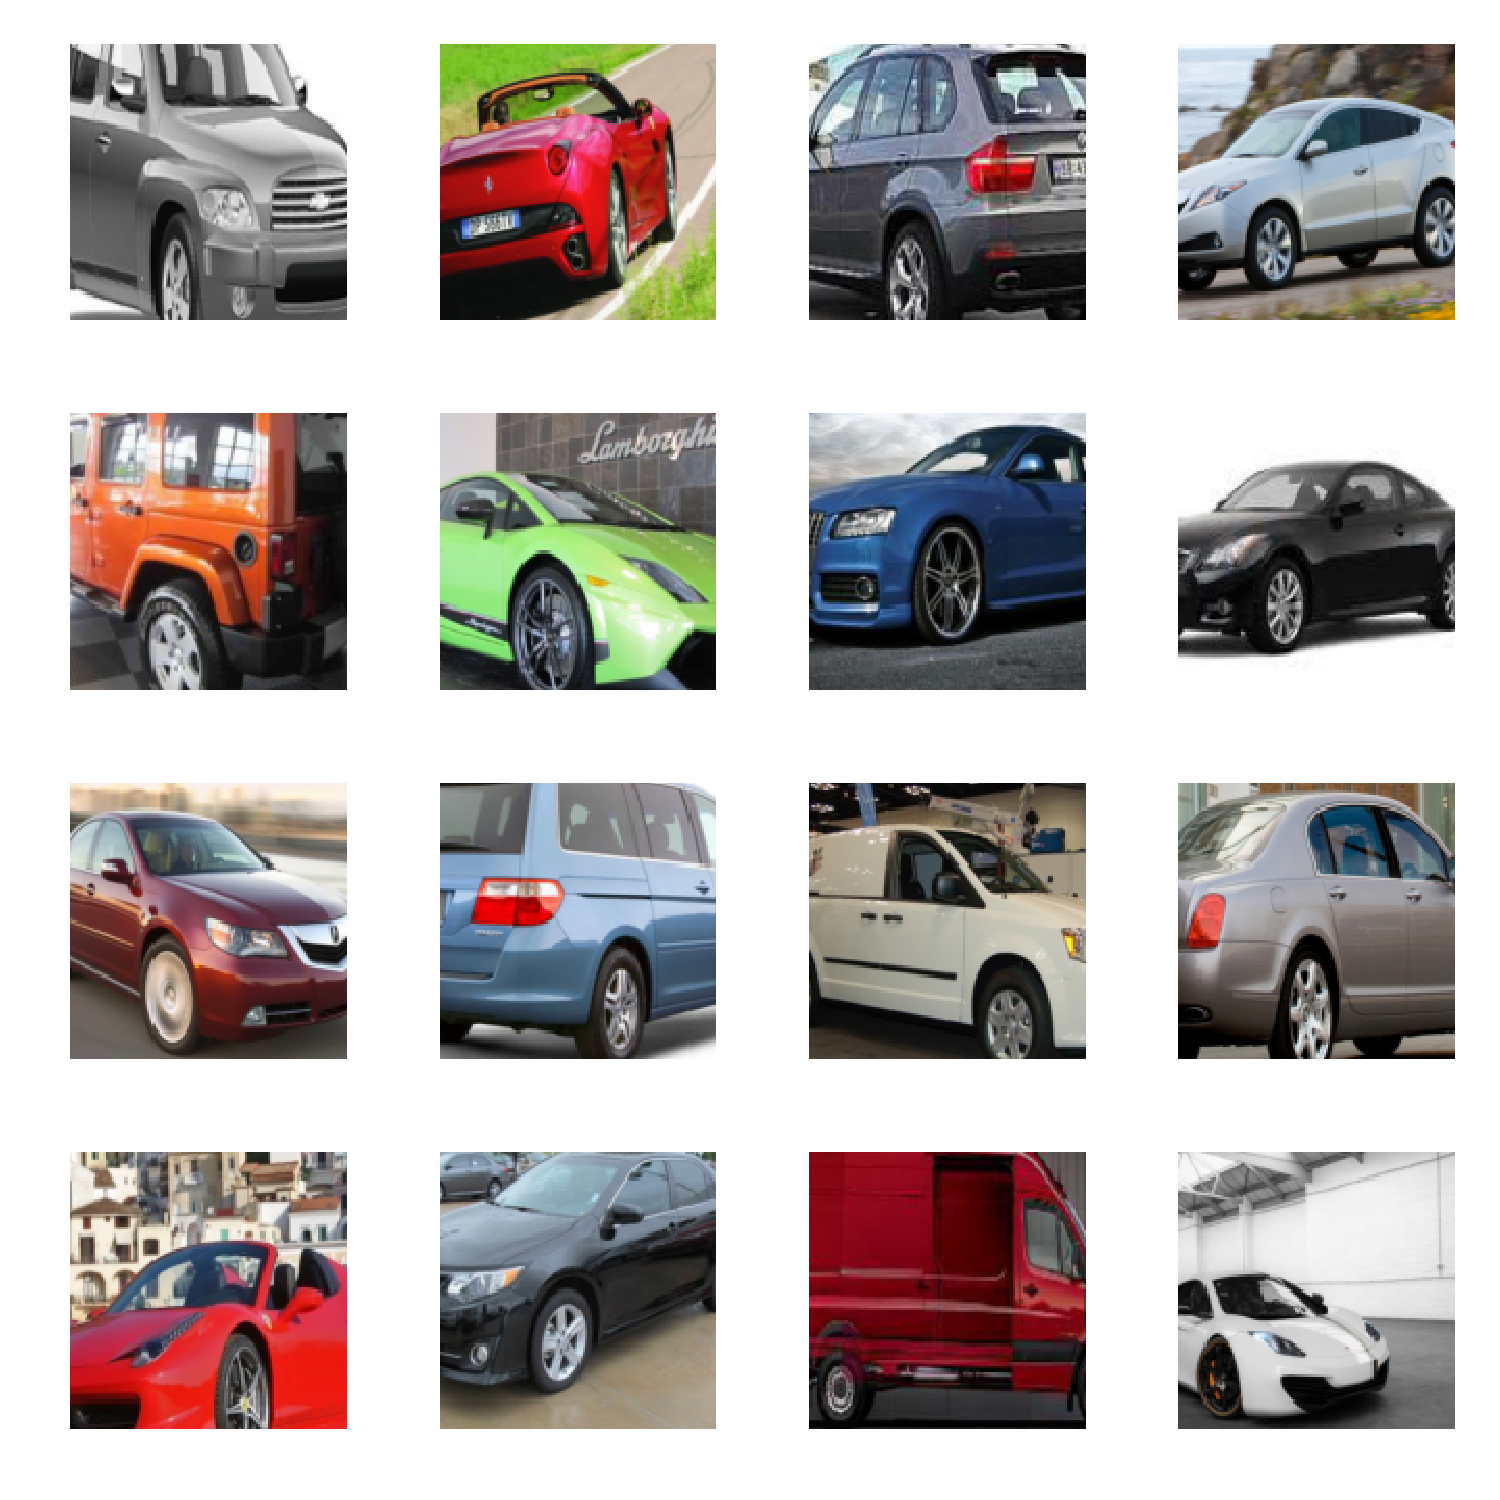
\includegraphics[width=6cm]{images/imagenet-inliers}
		\caption{Classe "normale"}
	\end{subfigure}
	\begin{subfigure}{6cm}
		\centering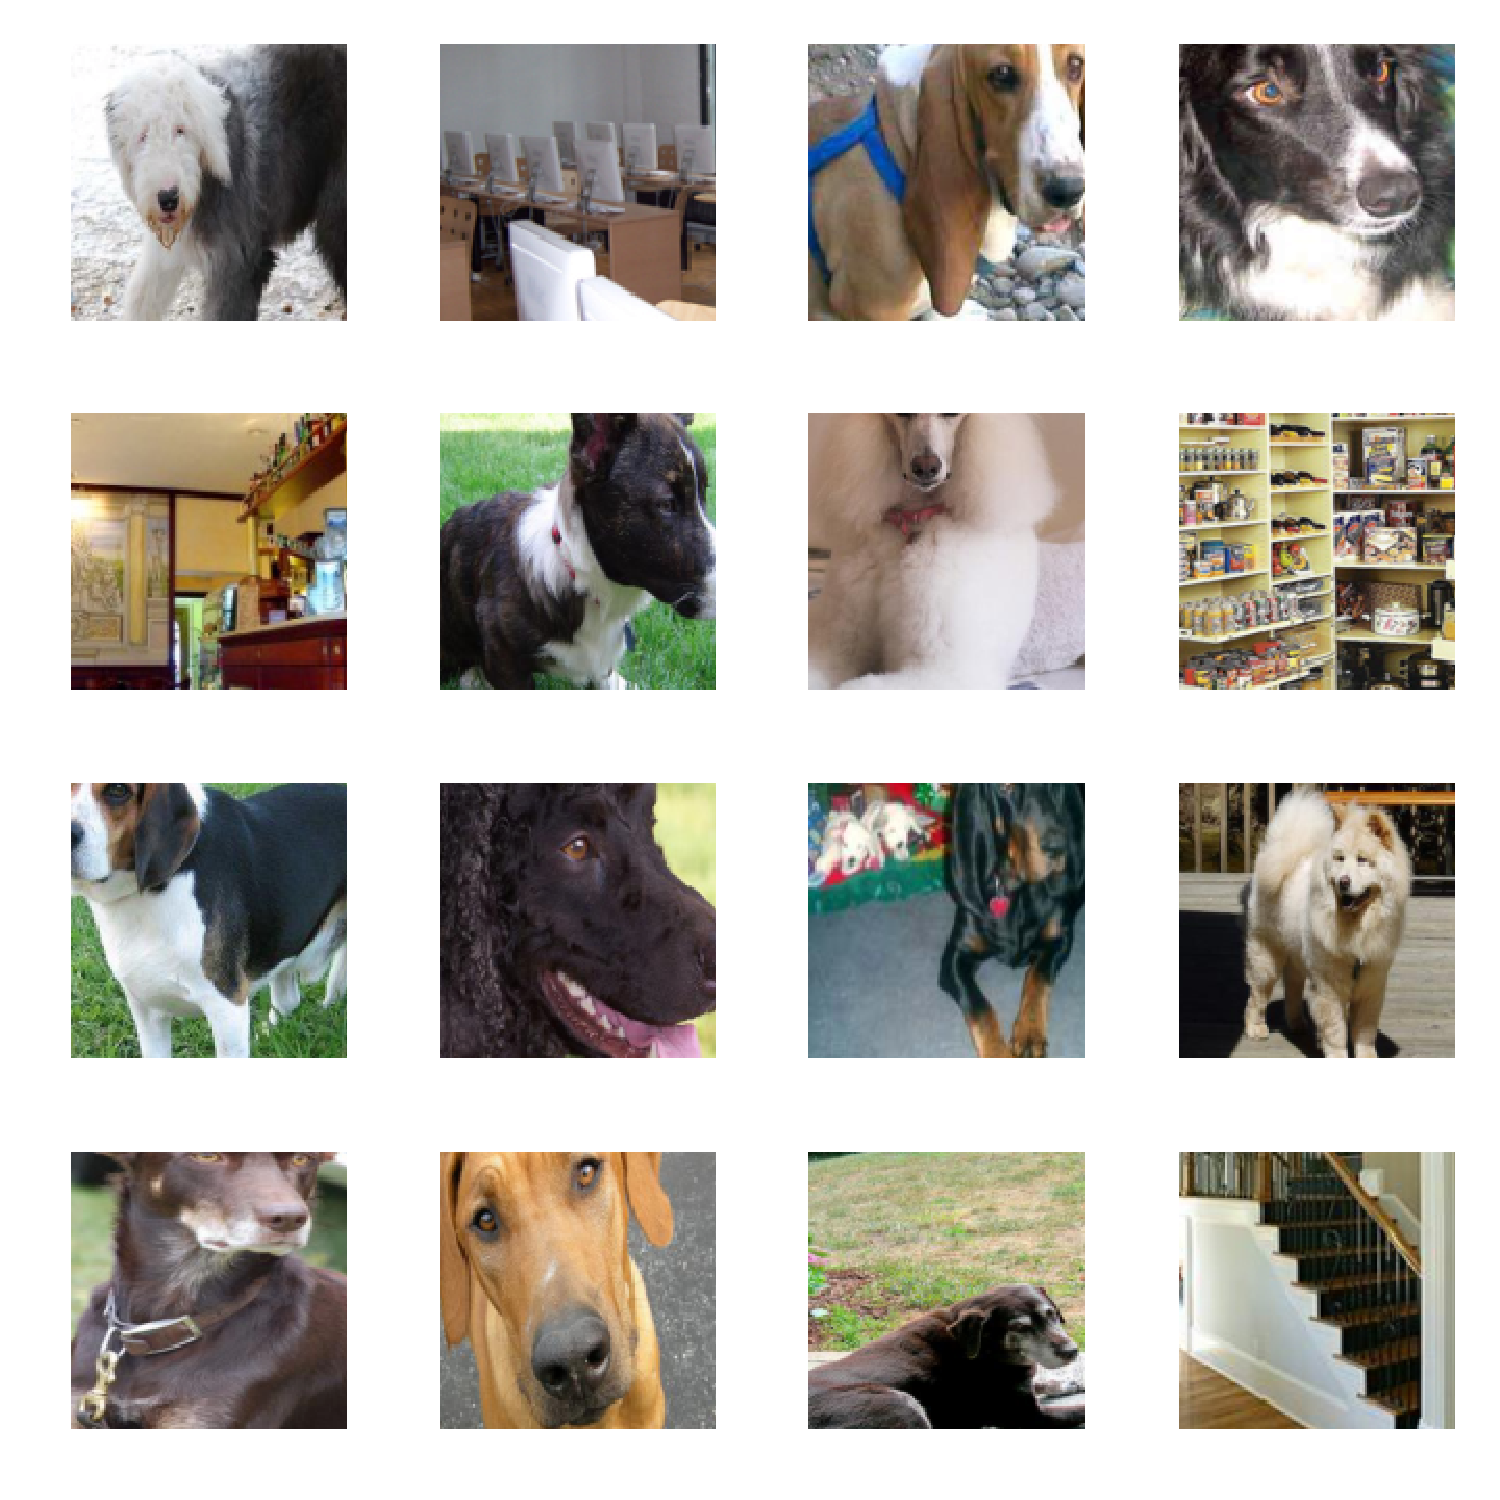
\includegraphics[width=6cm]{images/imagenet-outliers}
		\caption{Classe \DIFdelbeginFL \DIFdelFL{d'anomalies}\DIFdelendFL \DIFaddbeginFL \DIFaddFL{"anormale"}\DIFaddendFL }
	\end{subfigure}
	\caption{Exemples d'images pour notre jeu de données d'images réelles tirées de \textit{ImageNet}. La figure à gauche (a) correspond à des exemples de la classe dite "normale" et le volet de droite (b) correspond à des exemples de la classe d'anomalies.}
	\label{fig:imagenet}
\end{figure}

\begin{table}[h]
	\centering
	\caption{Description des \DIFdelbeginFL \DIFdelFL{2 }\DIFdelendFL \DIFaddbeginFL \DIFaddFL{deux }\DIFaddendFL ensembles de données pour le jeu de données de \textit{ImageNet}.}
	\begin{tabular}{| c | c | c | c |}
		\hline
		\rowcolor{Gray}
		Contamination & Ensemble de données  & Nombre d'instances & Pourcentage d'anomalies  \\
		\hline
		\multirow{2}{*}{Moins} 
		& $\mathcal{X}$ & 10000 & 10\%  \\
		& $\mathcal{X^*}$  & 1000 & 1\%  \\ 
		\midrule
		\multirow{2}{*}{Égal} 
		& $\mathcal{X}$ & 10000 & 5\%  \\
		& $\mathcal{X^*}$  & 1000 & 5\%  \\ 
		\midrule
		\multirow{2}{*}{Plus} 
		& $\mathcal{X}$ & 10000 & 1\%  \\
		& $\mathcal{X^*}$  & 1000 & 10\%  \\ 
		\midrule
	\end{tabular}
	\label{tab:dataset1}
\end{table}

Dans le cas du deuxième jeu de données, la classe "normale" est définie en prenant une catégorie du jeu de données \textit{MNIST}, soit un chiffre de 0 à 9. Nous avons ensuite défini \DIFdelbegin \DIFdel{3 }\DIFdelend \DIFaddbegin \DIFadd{trois }\DIFaddend scénarios de test différents. Ces \DIFdelbegin \DIFdel{3 }\DIFdelend \DIFaddbegin \DIFadd{trois }\DIFaddend scénarios se différencient par le nombre de classes que nous catégorisons comme des anomalies. Pour chacun de ces \DIFdelbegin \DIFdel{3 }\DIFdelend \DIFaddbegin \DIFadd{trois }\DIFaddend scénarios, nous avons testé \DIFdelbegin \DIFdel{2 }\DIFdelend \DIFaddbegin \DIFadd{deux }\DIFaddend catégories "normales" différentes, ce qui donne au total \DIFdelbegin \DIFdel{6 }\DIFdelend \DIFaddbegin \DIFadd{six }\DIFaddend scénarios de test. Ces scénarios sont définis \DIFdelbegin \DIFdel{plus en détails }\DIFdelend \DIFaddbegin \DIFadd{de manière plus détaillée }\DIFaddend dans le tableau \ref{tab:mnist_scenarios}. La figure \ref{fig:mnist} présente quelques exemples d'images, considérant que le chiffre \DIFdelbegin \DIFdel{0 }\DIFdelend \DIFaddbegin \DIFadd{1 }\DIFaddend est la classe "normale" et tous les autres chiffres sont des anomalies. Les images sont de type noir et blanc et sont toutes de dimensions 28 pixels par 28 pixels. Le tableau \ref{tab:dataset2} montre le nombre d'instances utilisées dans les jeux de données d'entraînement $\mathcal{X}$ et de test $\mathcal{X^*}$. Il montre également les proportions d'anomalies dans chaque ensemble, de la même manière qu'avec le jeu de données \textit{ImageNet}. Pour chacun des niveaux de contamination, les \DIFdelbegin \DIFdel{6 }\DIFdelend \DIFaddbegin \DIFadd{six }\DIFaddend différents scénarios du tableau \ref{tab:mnist_scenarios} ont été testés.

\begin{table}[h]
	\centering
	\caption{Description des \DIFdelbeginFL \DIFdelFL{2 ensembles }\DIFdelendFL \DIFaddbeginFL \DIFaddFL{six scénarios }\DIFaddendFL de \DIFdelbeginFL \DIFdelFL{données }\DIFdelendFL \DIFaddbeginFL \DIFaddFL{test effectués }\DIFaddendFL pour le jeu de données provenant de \textit{MNIST}.}
	\begin{tabular}{| a | a | a |}
		\hline
		\rowcolor{Gray}
		Scénario de test  & Chiffre "normal" & Chiffres "anormaux"  \\
		\hline
		1 & 1 & 5  \\
		2 & 1 & 5,9  \\
		3  & 1 & 0,2,3,4,5,6,7,8,9 \\ 
		4 & 6 & 8  \\
		5 & 6 & 3,8  \\
		6  & 6 & 0,1,2,3,4,5,7,8,9  \\ \hline
	\end{tabular}
	\label{tab:mnist_scenarios}
\end{table}

\begin{figure}[htb]
	\centering
	\begin{subfigure}{6cm}
		\centering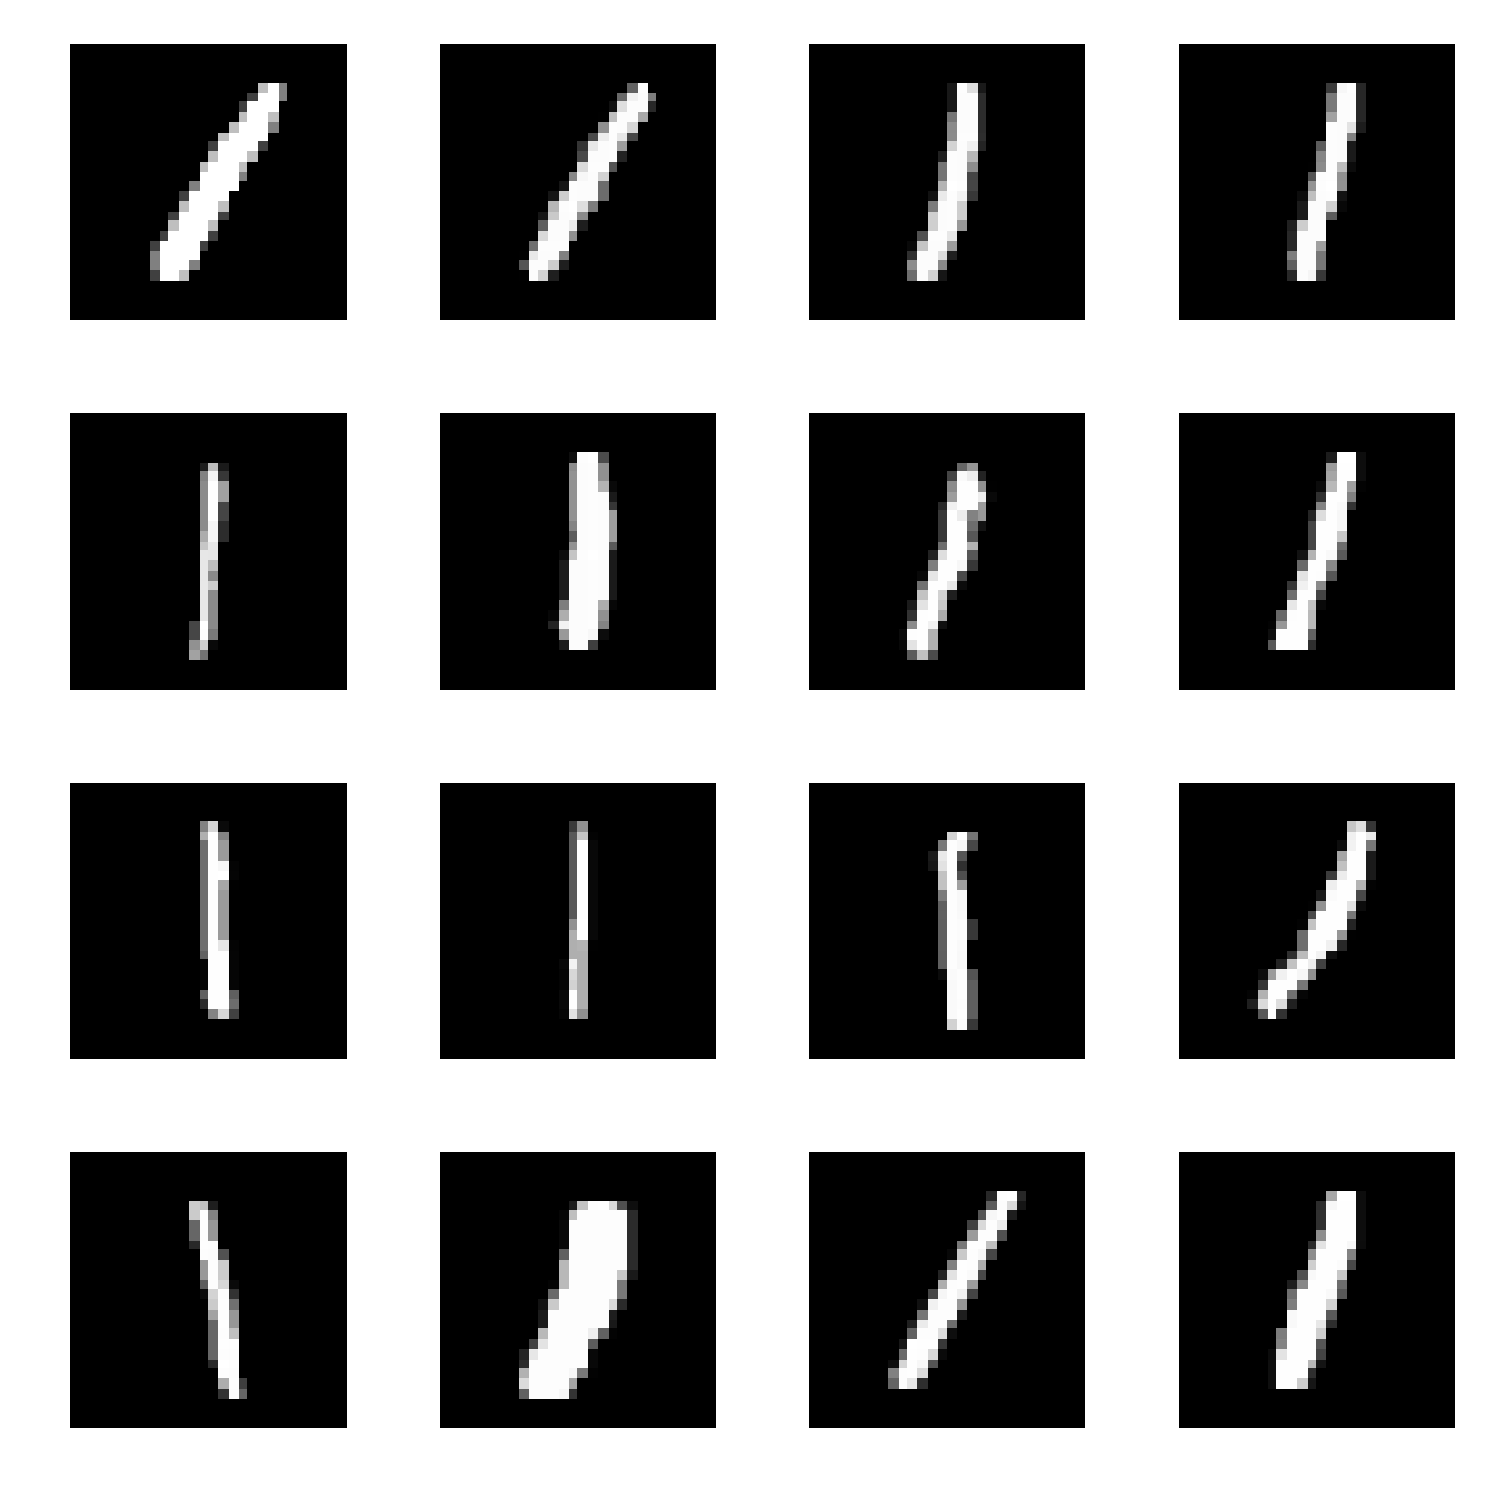
\includegraphics[width=6cm]{images/mnist-inliers}
		\caption{Classe normale}
	\end{subfigure}
	\begin{subfigure}{6cm}
		\centering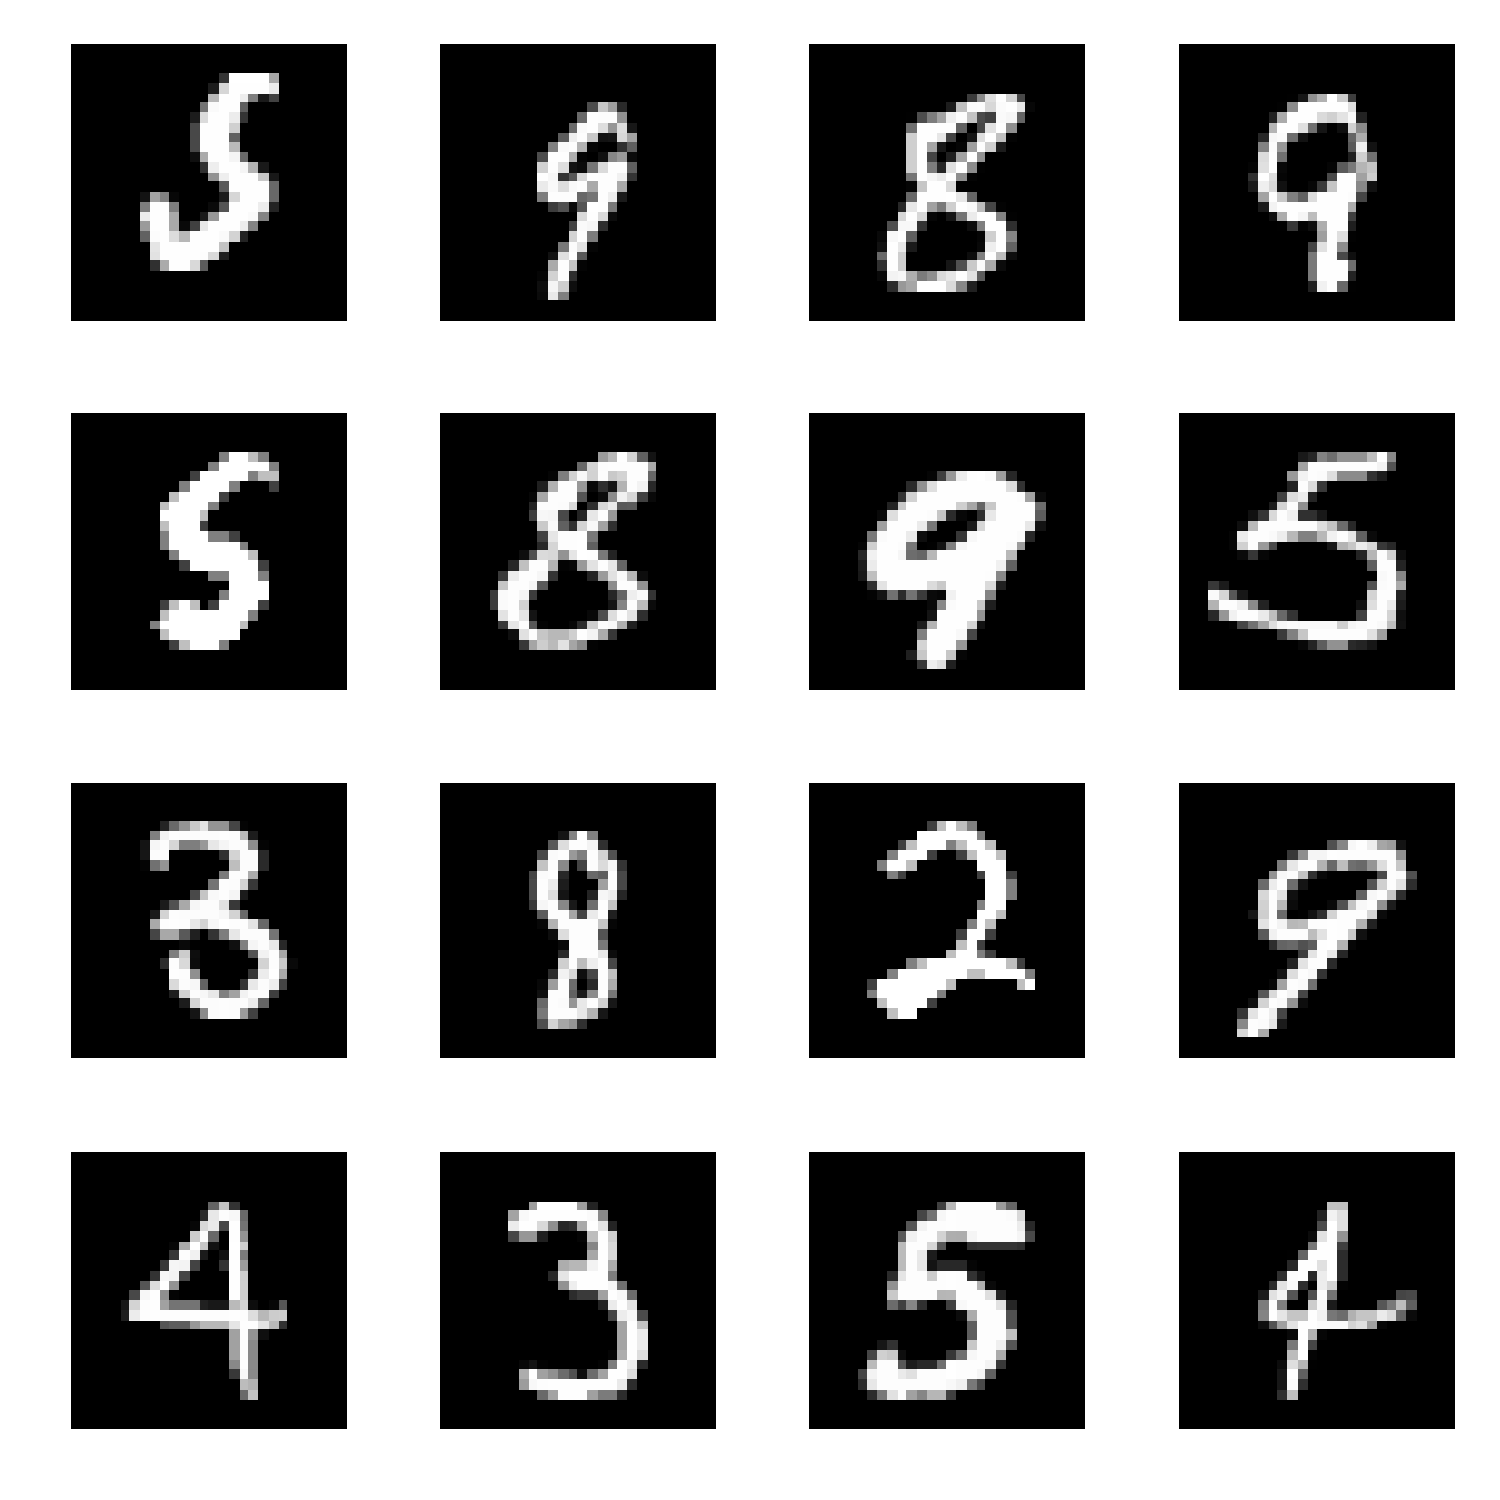
\includegraphics[width=6cm]{images/mnist-outliers}
		\caption{Classe \DIFdelbeginFL \DIFdelFL{d'anomalies}\DIFdelendFL \DIFaddbeginFL \DIFaddFL{"anormale"}\DIFaddendFL }
	\end{subfigure}
	\caption{Exemples d'images pour notre jeu de données \textit{MNIST}. La figure à gauche (a) correspond à des exemples de la classe "normale" et le volet de droite (b) correspond à des exemples de la classe d'anomalies. Il s'agit plus particulièrement du scénario de test 3.}
	\label{fig:mnist}
\end{figure}

\begin{table}[h]
	\centering
	\begin{tabular}{| c | c | c | c |}
		\hline
		\rowcolor{Gray}
		Contamination & Ensemble de données  & Nombre d'instances & Pourcentage d'anomalies  \\
		\hline
		\multirow{2}{*}{Moins} 
		& $\mathcal{X}$ & 4000 & 10\%  \\
		& $\mathcal{X^*}$  & 800 & 1\%  \\ 
		\midrule
		\multirow{2}{*}{Égal} 
		& $\mathcal{X}$ & 4000 & 5\%  \\
		& $\mathcal{X^*}$  & 800 & 5\%  \\ 
		\midrule
		\multirow{2}{*}{Plus} 
		& $\mathcal{X}$ & 4000 & 1\%  \\
		& $\mathcal{X^*}$  & 800 & 10\%  \\ 
		\midrule
	\end{tabular}
	\caption{Description des \DIFdelbeginFL \DIFdelFL{2 }\DIFdelendFL \DIFaddbeginFL \DIFaddFL{deux }\DIFaddendFL ensembles de données pour le jeu de données de \textit{MNIST}.}
	\label{tab:dataset2}
\end{table}

\section{Méthodes testées} \label{exp:methods}

Dans un premier temps, nous avons testé notre approche de détection d'anomalies basée sur des autoencodeurs variationnels, que nous appellerons DA-VAE (section \ref{DA_VAE}). Dans un deuxième temps, nous avons testé trois autres approches. Tout d'abord, nous avons testé une méthode basée sur une analyse en composantes principales (ACP), décrite plus en détails dans la section \ref{acp}. Ensuite, nous avons testé une approche basée sur un autoencodeur traditionnel avec des couches de convolutions (AE), décrite dans la section \ref{AE}. Finalement, nous avons testé une dernière approche utilisant le même autoencodeur variationnel que dans l'approche DA-VAE, mais en appliquant l'algorithme de détection d'anomalies \textit{Isolation Forest} \citep{4781136} sur les représentations latentes (ISOF-VAE). Cette méthode est décrite plus en détails dans la section \ref{isof_vae}. Ces quatre différentes approches et leurs détails d'entraînement sont approfondis dans les prochaines sous-sections.

\subsection{Détails sur la méthode DA-VAE} \label{DA_VAE}

La section \ref{chap:methodologie} décrit en détails le fonctionnement de l'approche que nous proposons. Par contre, certains détails concernant l'entraînement de l'autoencodeur variationnel ont été omis jusqu'à maintenant. Tout d'abord, il faut mentionner que l'architecture du réseau de neurones est différente pour chacun des \DIFdelbegin \DIFdel{2 }\DIFdelend \DIFaddbegin \DIFadd{deux }\DIFaddend jeux de données décrits à la section \ref{exp:datasets}.

Dans le cas du jeu de données provenant de \textit{ImageNet}, nous avons défini \DIFdelbegin \DIFdel{4 }\DIFdelend \DIFaddbegin \DIFadd{quatre }\DIFaddend couches de convolution pour l'encodeur et \DIFdelbegin \DIFdel{4 }\DIFdelend \DIFaddbegin \DIFadd{quatre }\DIFaddend couches de convolution transposée\DIFaddbegin \DIFadd{, ou de déconvolution, }\DIFaddend pour le décodeur. Chaque couche de convolution est suivie d'une normalisation par \DIFdelbegin \DIFdel{min-lot }\DIFdelend \DIFaddbegin \DIFadd{mini-lot }\DIFaddend (\textit{batch normalization}) et d'une fonction d'activation de type \textit{ReLU}. Juste avant de définir les couches de vecteurs latents $\boldsymbol{\mu}$ et $\boldsymbol{\sigma}$, le résultat de la dernière couche de convolution de l'encodeur, de dimensions $(512 \times 16 \times 16)$, est aplati en un vecteur de longueur 131 072. Les couches de vecteurs latents $\boldsymbol{\mu}$ et $\boldsymbol{\sigma}$ sont ensuite obtenues via une couche linéaire. La couche latente possède 25 dimensions. Nous avons entraîné le réseau sur 25 itérations complètes des données tout en ayant 130 observations par mini-lot. L'algorithme d'optimisation est celui de \textit{Adam} \citep{kingma2014method} et le taux d'apprentissage est de 0.001. Finalement, le niveau de filtration $\alpha$ appliqué sur le jeu de données de test est le même que la proportion de contamination dans le jeu de \DIFdelbegin \DIFdel{donnée }\DIFdelend \DIFaddbegin \DIFadd{données }\DIFaddend de test. La figure \ref{fig:archit_imagenet} présente en détails les différentes couches de l'encodeur et du décodeur.

\begin{figure}[htbp]
	\begin{subfigure}{12cm}
		\begin{tikzpicture}[shorten >=1pt,draw=black!50, node distance=\layersep, square/.style={regular polygon,regular polygon sides=4}]
		\tikzstyle{box}=[square,fill=white,minimum size=2cm,inner sep=-20pt, draw=black, text width=2.5cm, text centered]
		\tikzstyle{annot} = [text width=4em, text centered]

		% Draw different layers
		\node[box,fill=yellow!50] (input) at (0,0) {\tiny Entrée \\ $3 \PLH 128 \PLH 128$};
		\node[box,fill=green!50] (conv1) at (2,0) {\tiny Conv-2D $16 \PLH 128 \PLH 128$};
		\node[box,fill=green!50] (conv2) at (4,0) {\tiny Conv-2D $128 \PLH 64 \PLH 64$};
		\node[box,fill=green!50] (conv3) at (6,0) {\tiny Conv-2D $256 \PLH 32 \PLH 32$};
		\node[box,fill=green!50] (conv4) at (8,0) {\tiny Conv-2D $512 \PLH 16 \PLH 16$};
		\node[box,fill=yellow!50] (flatten) at (10,0) {\tiny Flatten \\ $1 \PLH 131 072$};
		\node[box,fill=black!30] (mu) at (12,1.2) {\tiny Linéaire \\ $1 \PLH 25$};
		\node[box,fill=black!30] (sigma) at (12,-1.2) {\tiny Linéaire \\ $1 \PLH 25$};
		\node[box,fill=yellow!50] (z) at (14,0) {\tiny $z$ \\ $1 \PLH 25$};

		% Draw arrows
		\path[->, line width=1mm] (input) edge (conv1);
		\path[->, line width=1mm] (conv1) edge (conv2);
		\path[->, line width=1mm] (conv2) edge (conv3);
		\path[->, line width=1mm] (conv3) edge (conv4);
		\path[->, line width=1mm] (conv4) edge (flatten);
		\path[->, line width=1mm] (flatten) edge (mu);
		\path[->, line width=1mm] (flatten) edge (sigma);
		\path[->, line width=1mm] (mu) edge (z);
		\path[->, line width=1mm] (sigma) edge (z);

		\node[annot,above of=mu, node distance=1cm] (h2) {$\mu$};
		\node[annot,above of=sigma, node distance=1cm] (h3) {$\sigma$};

		\end{tikzpicture}
		\caption{Architecture de l'encodeur}
	\end{subfigure}
	\begin{subfigure}{12cm}
		\vspace{0.75cm}
		\begin{tikzpicture}[shorten >=1pt,draw=black!50, node distance=\layersep, square/.style={regular polygon,regular polygon sides=4}]
		\tikzstyle{box}=[square,fill=white,minimum size=2cm,inner sep=-20pt, draw=black, text width=2.5cm, text centered]
		\tikzstyle{annot} = [text width=4em, text centered]

		% Draw different layers
		\node[box,fill=yellow!50] (z) at (0,0) {\tiny $z$ \\ $1 \PLH 25$};
		\node[box,fill=black!30] (linear3) at (2,0) {\tiny Linéaire \\ $1 \PLH 131 072$};
		\node[box,fill=yellow!50] (unflatten) at (4,0) {\tiny Unflatten \\ $512 \PLH 16 \PLH 16$};
		\node[box,fill=green!50] (deconv1) at (6,0) {\tiny Deconv-2D $256 \PLH 32 \PLH 32$};
		\node[box,fill=green!50] (deconv2) at (8,0) {\tiny Deconv-2D $128 \PLH 64 \PLH 64$};
		\node[box,fill=green!50] (deconv3) at (10,0) {\tiny Deconv-2D $16 \PLH 128 \PLH 128$};
		\node[box,fill=green!50] (deconv4) at (12,0) {\tiny Deconv-2D $3 \PLH 128 \PLH 128$};
		\node[box,fill=yellow!50] (output) at (14,0) {\tiny Sortie \\ $3 \PLH 128 \PLH 128$};

		% Draw arrows
		\path[->, line width=1mm] (z) edge (linear3);
		\path[->, line width=1mm] (linear3) edge (unflatten);
		\path[->, line width=1mm] (unflatten) edge (deconv1);
		\path[->, line width=1mm] (deconv1) edge (deconv2);
		\path[->, line width=1mm] (deconv2) edge (deconv3);
		\path[->, line width=1mm] (deconv3) edge (deconv4);
		\path[->, line width=1mm] (deconv4) edge (output);

		\end{tikzpicture}
		\vspace{0.15cm}
		\caption{Architecture du décodeur}
	\end{subfigure}
	\caption{Architecture du modèle DA-VAE pour le jeu de données \textit{ImageNet}. Les blocs représentent les couches du réseau. Les blocs jaunes représentent les couches où il n'y a pas de paramètres à optimiser. Les blocs verts sont des couches de convolution ou déconvolution et les blocs gris sont des couches linéaires. }
	\label{fig:archit_imagenet}
\end{figure}

Pour le jeu de données provenant de \textit{MNIST}, nous avons défini \DIFdelbegin \DIFdel{3 }\DIFdelend \DIFaddbegin \DIFadd{trois }\DIFaddend couches de convolution pour l'encodeur et 3 couches de convolution transposée pour le décodeur. Nous avons fait le choix de mettre moins de couches que dans le cas du jeu de données \textit{ImageNet} en raison de la complexité moins importante des données.  Chaque couche de convolution est suivie d'une fonction d'activation de type \textit{ReLU}. Chaque couche de convolution de l'encodeur est également suivie d'un \textit{max pooling} de dimensions $2 \times 2$. Juste avant de définir les couches de vecteurs latents $\boldsymbol{\mu}$ et $\boldsymbol{\sigma}$, le résultat de la dernière couche de convolution de l'encodeur, de dimensions $(64 \times 4 \times 4)$, est aplati en un vecteur  de longueur 1024. Les couches de vecteurs latents $\boldsymbol{\mu}$ et $\boldsymbol{\sigma}$ sont ensuite obtenues via une couche linéaire. La couche latente possède 25 dimensions. Nous avons entraîné le réseau pendant 75 itérations complètes des données tout en ayant 256 observations par mini-lot. L'algorithme d'optimisation est celui de \textit{Adam} et le taux d'apprentissage est de 0.001. Finalement, le niveau de filtration $\alpha$ appliqué sur le jeu de données de test est le même que la proportion de contamination dans l'ensemble de données de test. La figure \ref{fig:archit_mnist} présente en détails les différentes couches de l'encodeur et du décodeur.

\begin{figure}[htbp]
	\begin{subfigure}{12cm}
		\begin{tikzpicture}[shorten >=1pt,draw=black!50, node distance=\layersep, square/.style={regular polygon,regular polygon sides=4}]
		\tikzstyle{box}=[square,fill=white,minimum size=2cm,inner sep=-19pt, draw=black, text width=2.5cm, text centered]
		\tikzstyle{annot} = [text width=4em, text centered]

		% Draw different layers
		\node[box,fill=yellow!50] (input) at (0,0) {\tiny Entrée \\ $1 \PLH 28 \PLH 28$};
	\node[box,fill=green!50] (conv1) at (2,0) {\tiny Conv-2D + \\ Max-pooling $16 \PLH 14 \PLH 14$};
		\node[box,fill=green!50] (conv2) at (4,0) {\tiny Conv-2D + \\ Max-pooling $32 \PLH 7 \PLH 7$};
		\node[box,fill=green!50] (conv3) at (6,0) {\tiny 0-padding \\ $32 \PLH 8 \PLH 8$};
		\node[box,fill=green!50] (conv4) at (8,0) {\tiny Conv-2D + \\ Max-pooling $64 \PLH 4 \PLH 4$};
		\node[box,fill=yellow!50] (flatten) at (10,0) {\tiny Flatten \\ $1 \PLH 1024$};
		\node[box,fill=black!30] (mu) at (12,1.2) {\tiny Linéaire \\ $1 \PLH 25$};
		\node[box,fill=black!30] (sigma) at (12,-1.2) {\tiny Linéaire \\ $1 \PLH 25$};
		\node[box,fill=yellow!50] (z) at (14,0) {\tiny $z$ \\ $1 \PLH 25$};

		% Draw arrows
		\path[->, line width=1mm] (input) edge (conv1);
		\path[->, line width=1mm] (conv1) edge (conv2);
		\path[->, line width=1mm] (conv2) edge (conv3);
		\path[->, line width=1mm] (conv3) edge (conv4);
		\path[->, line width=1mm] (conv4) edge (flatten);
		\path[->, line width=1mm] (flatten) edge (mu);
		\path[->, line width=1mm] (flatten) edge (sigma);
		\path[->, line width=1mm] (mu) edge (z);
		\path[->, line width=1mm] (sigma) edge (z);

		\node[annot,above of=mu, node distance=1cm] (h2) {$\mu$};
		\node[annot,above of=sigma, node distance=1cm] (h3) {$\sigma$};

		\end{tikzpicture}
		\caption{Architecture de l'encodeur}
	\end{subfigure}
	\begin{subfigure}{12cm}
		\vspace{0.75cm}
		\begin{tikzpicture}[shorten >=1pt,draw=black!50, node distance=\layersep, square/.style={regular polygon,regular polygon sides=4}]
		\tikzstyle{box}=[square,fill=white,minimum size=2cm,inner sep=-20pt, draw=black, text width=2.5cm, text centered]
		\tikzstyle{annot} = [text width=4em, text centered]

		% Draw different layers
		\node[box,fill=yellow!50] (z) at (0,0) {\tiny $z$ \\ $1 \PLH 25$};
		\node[box,fill=black!30] (linear3) at (2,0) {\tiny Linéaire \\ $1 \PLH 1024$};
		\node[box,fill=yellow!50] (unflatten) at (4,0) {\tiny Unflatten \\ $64 \PLH 4 \PLH 4$};
		\node[box,fill=green!50] (deconv1) at (6,0) {\tiny Deconv-2D \\ $64 \PLH 8 \PLH 8$};
		\node[box,fill=green!50] (deconv2) at (8,0) {\tiny Deconv-2D \\ $32 \PLH 16 \PLH 16$};
		\node[box,fill=green!50] (deconv3) at (10,0) {\tiny Deconv-2D \\ $16 \PLH 28 \PLH 28$};
		\node[box,fill=green!50] (deconv4) at (12,0) {\tiny Conv-2D \\ $1 \PLH 28 \PLH 28$};
		\node[box,fill=yellow!50] (output) at (14,0) {\tiny Sortie \\ $1 \PLH 28 \PLH 28$};

		% Draw arrows
		\path[->, line width=1mm] (z) edge (linear3);
		\path[->, line width=1mm] (linear3) edge (unflatten);
		\path[->, line width=1mm] (unflatten) edge (deconv1);
		\path[->, line width=1mm] (deconv1) edge (deconv2);
		\path[->, line width=1mm] (deconv2) edge (deconv3);
		\path[->, line width=1mm] (deconv3) edge (deconv4);
		\path[->, line width=1mm] (deconv4) edge (output);

		\end{tikzpicture}
		\vspace{0.15cm}
		\caption{Architecture du décodeur}
	\end{subfigure}
	\caption{Architecture du modèle DA-VAE pour le jeu de données provenant de \textit{MNIST}. Les blocs représentent les couches du réseau. Les blocs jaunes représentent les couches où il n'y a pas de paramètres à optimiser. Les blocs verts sont des couches de convolution ou déconvolution et les blocs gris sont des couches linéaires.}
	\label{fig:archit_mnist}
\end{figure}

\subsubsection{Horaire du paramètre $\beta$} \label{beta_schedule}

Dans les deux expériences différentes, nous avons traité le paramètre $\beta$ d'une manière particulière. En effet, étant donné que nous utilisons des $\beta$-VAE, nous devons définir un paramètre $\beta$ qui donne plus ou moins d'importance à la composante de perte associée au critère de \DIFdelbegin \DIFdel{Kulbach-Leibler }\DIFdelend \DIFaddbegin \DIFadd{Kulback-Leibler }\DIFaddend (voir section \ref{beta-vae}). Dans notre cas, nous n'avons pas conservé ce paramètre $\beta$ fixe tout au long de l'entraînement. Pour l'entraînement des \DIFdelbegin \DIFdel{2 }\DIFdelend \DIFaddbegin \DIFadd{deux }\DIFaddend différents jeux de données, nous avons donc mis en place un horaire du paramètre $\beta$ selon l'itération d'entraînement\DIFdelbegin \DIFdel{(ou }\textit{\DIFdel{epoch}}%DIFAUXCMD
\DIFdel{)}\DIFdelend . Cet horaire n'est pas le même selon le jeu de données et a été choisi en se basant sur la section 3.1 de l'article de \cite{bowman-etal-2016-generating}. Ce qui est proposé dans cet article est de commencer l'entraînement en attribuant un poids de zéro à la perte de KL. Pendant les premières itérations, le réseau va donc optimiser ses paramètres en fonction de la composante de reconstruction seulement. Par la suite, on augmente le paramètre $\beta$ pour régulariser le modèle et ainsi rapprocher les paramètres $\boldsymbol{\mu}$ et $\boldsymbol{\sigma}$ de ceux de la $N(0,I)$. Le tableau \ref{tab:betas} présente les paramètres $\beta$ utilisés selon l'itération \DIFdelbegin \DIFdel{(}\textit{\DIFdel{epoch}}%DIFAUXCMD
\DIFdel{) }\DIFdelend d'entraînement et le jeu de données.

\begin{table}[h]
	\centering
	\caption{Horaire des paramètres $\beta$ pour le jeu de données provenant de \textit{ImageNet} et le jeu de données provenant de \textit{MNIST}.}
	\begin{tabular}{| a | a | a |}
		\hline
		\rowcolor{Gray}
		Itération  & $\beta_{ImageNet}$ & $\beta_{MNIST}$  \\
		\hline
		$[0,5]$ & 0 & 0  \\
		$[6,10]$  & 100 & 10  \\
		$[11,\infty]$  & 10 & 1  \\ \hline

	\end{tabular}
	\label{tab:betas}
\end{table}

L'intuition derrière l'horaire établi est de contrôler le modèle dans les premières itérations pour éviter d'accorder trop d'importance, et ce trop rapidement, à la composante de régularisation KL. Cela pourrait avoir comme conséquence de nuire au reste de l'optimisation et à l'apprentissage de la composante de reconstruction.	

\subsection{Détails sur la méthode ACP} \label{acp}

Une première approche testée pour comparer nos résultats consiste à effectuer une analyse en composantes principales (ACP). L'objectif premier de cette technique non-supervisée est de réduire la dimension d'un ensemble de données en conservant le plus d'information possible. Cela permet d'ailleurs de représenter les données dans un espace plus simple sous formes de représentations latentes. Il est aussi possible de reconstruire ces représentations dans les dimensions originales, \DIFaddbegin \DIFadd{tel que vu à la sous-section \ref{soussec:linear}, }\DIFaddend et ainsi de calculer un score d'anomalie basé sur la capacité de bien reconstruire. Dans cette méthode, les valeurs et vecteurs propres de la matrice de covariance des variables standardisées 

\begin{equation} \label{eq1}
	\begin{split}
		\hat{\text{var}}(\mathbf{X}) & = \frac{1}{n}\mathbf{X}^{T}\mathbf{X},
	\end{split}
\end{equation}


nous permettent d'obtenir une projection de cette matrice dans un espace à plus petites dimensions. La matrice $\mathbf{X}$ correspond aux données standardisées dont on cherche à réduire la dimension. La matrice de vecteurs propres $\mathbf{V}$ est de dimensions \DIFdelbegin \DIFdel{$p \times d$}\DIFdelend \DIFaddbegin \DIFadd{$p \times k$}\DIFaddend , où $p$ correspond au nombre de variables de la matrice $\mathbf{X}$ et \DIFdelbegin \DIFdel{$d$ }\DIFdelend \DIFaddbegin \DIFadd{$k$ }\DIFaddend correspond au nombre de composantes principales conservées dans l'espace réduit. La représentation en dimension réduite, soit $\mathbf{Z}$, est obtenue par le produit de $\mathbf{X}\mathbf{\mathbf{V}}$. Finalement, la reconstruction dans l'espace original, $\hat{\mathbf{X}}$, est donnée par \DIFaddbegin \DIFadd{$\hat{\mathbf{X}} = \mathbf{Z}\mathbf{V}^{T}$.
}\DIFaddend 

\DIFdelbegin \begin{eqnarray*}
	\DIFdel{\hat{\mathbf{X}} = \mathbf{Z}\mathbf{V}^{T}=\mathbf{X}\mathbf{V}\mathbf{V}^{T}.
}\end{eqnarray*}
%DIFAUXCMD
%DIFDELCMD < 

%DIFDELCMD < %%%
\DIFdelend Étant donné que nos données sont des images, ou des matrices en plusieurs dimensions, nous avons aplati chacune des entrées pour obtenir des vecteurs. Dans le cas des images en couleur provenant de \textit{ImageNet}, nous avons d'abord aplati chacun des canaux RGB. Ensuite, nous avons fait une analyse en composantes principales sur chaque canal RGB séparément. Chaque canal image est de dimensions $1 \times 128 \times 128$, ce qui veut dire que nous obtenons un vecteur de longueur 16 384 pour chaque ACP. Pour les images provenant de \textit{MNIST}, les images sont de dimensions $1 \times 28 \times 28$, ce qui nous donne des vecteurs de longueur 784. Cette vectorisation est nécessaire dans le cas de l'analyse en composantes principales puisque chaque observation de $\mathbf{X}$ doit être représentée comme un vecteur.

Pour trouver les anomalies, nous avons utilisé l'erreur de reconstruction entre les données originales $(x^{*(j)})_{j=1}^k$ et
leur reconstruction $(\hat{x}^{*(j)})_{j=1}^k$ basée uniquement sur un certain nombre de composantes principales. Dans nos expériences, ce nombre de composantes principales \DIFdelbegin \DIFdel{à }\DIFdelend \DIFaddbegin \DIFadd{a }\DIFaddend été établi afin d'obtenir une projection conservant approximativement 80\% de la variance originale des données. Nous avons utilisé l'erreur quadratique moyenne comme erreur de reconstruction. Une observation $x^{*(j)}$ est considérée comme une anomalie au niveau de filtration $\alpha$ si

\begin{gather} \label{eq:anomalie_mse}
l(x^{*(j)}, \hat{x}^{*(j)}) > t_{1-\alpha}(L(\mathcal{X}, \hat{\mathcal{X}})),
\end{gather}

où $l(x^{*(j)}, \hat{x}^{*(j)})$ correspond à l'erreur de reconstruction pour l'observation $i$ du jeu de données test $\mathcal{X^*}$ et $t_{1-\alpha}(L(\mathcal{X}, \hat{\mathcal{X}}))$ correspond au percentile $1-\alpha$ de l'ensemble des erreurs de reconstruction sur le jeu de données d'entraînement $\mathcal{X}$. Dans le cas de l'ACP appliquée sur \textit{ImageNet}, nous avons calculé l'erreur de reconstruction sur chaque canal indépendamment pour ensuite prendre la moyenne des \DIFdelbegin \DIFdel{3 }\DIFdelend \DIFaddbegin \DIFadd{trois }\DIFaddend erreurs de reconstruction. Le niveau de filtration $\alpha$ choisi est le même que la proportion de contamination dans l'ensemble de données de test. Nous avons \DIFdelbegin \DIFdel{fait }\DIFdelend \DIFaddbegin \DIFadd{choisi }\DIFaddend cela afin de mettre toutes les méthodes comparatives sur le même pied d'égalité. Nous avons donc fixé cette même valeur de $\alpha$ pour les \DIFdelbegin \DIFdel{2 }\DIFdelend \DIFaddbegin \DIFadd{deux }\DIFaddend autres méthodes comparatives. \DIFdelbegin \DIFdel{Nous }\DIFdelend \DIFaddbegin \DIFadd{De plus, nous }\DIFaddend avons choisi $\alpha$ égal à la vraie proportion de contamination du jeu de données test afin de comparer les méthodes dans une situation plus simple.

Pour le jeu de données \textit{ImageNet}, nous avons conservé le nombre de composantes principales nous permettant de conserver exactement 80 \% de la variabilité pour chaque canal RGB. Ce nombre de composantes principales peut donc varier légèrement selon le canal et l'échantillonnage du jeu de données et prend des valeurs entre 90 et \DIFdelbegin \DIFdel{110 dans cette application. }\DIFdelend \DIFaddbegin \DIFadd{110. }\DIFaddend Pour le jeu de données \textit{MINST}, nous avons toujours conservé les 30 premières composantes principales. Cela nous permet de conserver approximativement  80 \% de la variabilité. 

\subsection{Détails sur la méthode AE} \label{AE}

Une deuxième approche testée consiste à utiliser un autoencodeur traditionnel et de se servir de l'erreur de reconstruction comme score d'anomalie. Pour cette approche, nous avons utilisé les mêmes architectures que celles définies dans la section \ref{DA_VAE}, mais sans les couches linéaires latentes du réseau DA-VAE. Par exemple, pour l'autoencodeur appliqué sur les images provenant de \textit{ImageNet}, nous avons conservé les \DIFdelbegin \DIFdel{4 }\DIFdelend \DIFaddbegin \DIFadd{quatre }\DIFaddend premières couches de convolution et avons ensuite appliqué les \DIFdelbegin \DIFdel{4 }\DIFdelend \DIFaddbegin \DIFadd{quatre }\DIFaddend dernières couches de convolution transposée immédiatement après. Il n'y a donc pas de vectorisation qui est nécessaire. 

Nous avons utilisé l'erreur quadratique moyenne comme erreur de reconstruction. Les anomalies du jeu de données test $\mathcal{X^*}$ sont donc prédites de façon similaire à ce qui est présenté à l'équation \ref{eq:anomalie_mse}. Comme pour les autres méthodes, le niveau de filtration $\alpha$ choisi est le même que la proportion de contamination dans le jeu de données de test. 

\subsection{Détails sur la méthode ISOF-VAE} \label{isof_vae}

Finalement, nous avons testé une dernière approche qui consiste à utiliser différemment les représentations latentes du réseau entraîné avec l'approche DA-VAE. Au lieu de calculer une distance de Kullback-Leibler entre chaque représentation latente et une distribution normale $N(0,I)$, nous utiliserons ici les représentations latentes pour entraîner l'algorithme \textit{Isolation Forest}. Cet algorithme non-supervisé, principalement utilisé en détection d'\DIFdelbegin \DIFdel{anomalie}\DIFdelend \DIFaddbegin \DIFadd{anomalies}\DIFaddend , utilise plusieurs arbres de décisions binaires regroupés dans ce qu'on appelle une forêt d'arbres. Chacun des arbres est entraîné sur un certain nombre d'observations tirées au hasard et avec remise. De plus, il est également possible de tirer au hasard un certains nombre de variables pour entraîner chacun des arbres. Ce processus est très similaire à ce qui est fait en apprentissage supervisé avec les forêts aléatoires \citep{Statistics01randomforests}. L'hypothèse de base de cet algorithme quant aux anomalies est fondée autour du fait qu'elles sont peu nombreuses et possèdent des caractéristiques différentes des observations "normales". Sachant cette hypothèse, ces anomalies sont susceptibles d'être isolées dans les premières séparations des arbres de décisions. Pour déterminer si une observation est isolée, on calcule le nombre de nœuds à parcourir dans l'arbre pour atteindre cette observation. Plus ce chemin est petit, plus l'observation risque d'être une anomalie.

Afin d'obtenir un score d'anomalie comparable à notre niveau de filtration $\alpha$, nous avons légèrement transformé le score d'anomalie calculé par l'algorithme. Pour une observation donnée, le score d'anomalie $S$  calculé par l'algorithme est obtenu en prenant la moyenne du nombre de nœuds parcouru dans chacun des arbres de la forêt pour atteindre cette observation. Plus ce score est petit, plus l'observation est susceptible d'être isolée et d'être considérée "anormale". Pour être en mesure de comparer ce score avec notre niveau de filtration, nous avons d'abord calculé ce score pour chacune des $n$ observations de notre jeu de données d'entraînement, ce que nous appelons l'ensemble $S_{\mathcal{X}} = \{S^{(1)}, ..., S^{(n)}\}$. Nous définissons également $S^{'}_{\mathcal{X}}$ comme l'ensemble $S_{\mathcal{X}}$ ordonné en ordre croissant.  Ensuite, nous avons défini notre propre score d'anomalie $S^*(\cdot)$ pour une observation du jeu de donnée de test $x^{*(j)}$ comme suit,

\begin{gather}
	S^*(x^{*(j)}) = \frac{rang_{S^{'}_{\mathcal{X}}}(S^{(j)})}{n},
\end{gather}

où $rang_{S^{'}_{\mathcal{X}}}(S^{(j)})$ correspond au rang du score $S^{(j)}$ de l'observation $x^{*(j)}$ dans l'ensemble ordonné $S^{'}_{\mathcal{X}}$. Ce score $S^*(x^{*(j)})$, peut être comparé à notre niveau de filtration $\alpha$. Ce niveau de filtration choisi est le même que la proportion de contamination dans le jeu de données de test.

\section{Résultats} \label{exp:results}

Pour comparer les différentes méthodes, nous avons utilisé \DIFdelbegin \DIFdel{3 }\DIFdelend \DIFaddbegin \DIFadd{trois }\DIFaddend métriques différentes. La première est l'aire sous la courbe ROC. Cette métrique nous permet de faire abstraction du seuil de filtration $\alpha$. Ensuite, nous avons également choisi les métriques de précision et de rappel, qui prennent en considération un certain seuil, $\alpha$ dans notre cas. Nous avons entraîné et testé les algorithmes à 20 reprises, ce qui nous permet de calculer une moyenne et une mesure de dispersion, soit l'écart-type, autour de chacune des métriques. Pour les 20 réplications, l'échantillonnage des jeux de données de test et d'entraînement est refait. La variabilité des résultats entre les 20 réplications est expliquée par \DIFdelbegin \DIFdel{3 }\DIFdelend \DIFaddbegin \DIFadd{trois }\DIFaddend composantes :

\begin{enumerate}
	\item L'échantillonnage des jeux de données;
	\item L'initialisation des paramètres et l'optimisation par descente du gradient dans les réseaux de neurones;
	\item La composante stochastique dans la représentation latente du VAE.
\end{enumerate}

La première composante, soit l'échantillonnage des jeux de données, affecte les \DIFdelbegin \DIFdel{4 }\DIFdelend \DIFaddbegin \DIFadd{quatre }\DIFaddend différents algorithmes. La deuxième composante, soit l'initialisation des paramètres et l'optimisation par descente du gradient, n'affecte que les méthodes reliées à des réseaux de neurones: DA-VAE(\ref{DA_VAE}), AE (\ref{AE}) et ISOF-VAE (\ref{isof_vae}). La composante stochastique dans l'optimisation par descente du gradient est reliée au fait que le jeu de données d'entraînement est divisé en sous-ensembles, aussi appelés \DIFdelbegin \DIFdel{mini-lot}\DIFdelend \DIFaddbegin \DIFadd{mini-lots}\DIFaddend , qui sont définis aléatoirement. Ces sous-ensembles sont utilisés pour calculer les pertes sur lesquelles on calcule les dérivés permettant de mettre à jour les paramètres de l'autoencodeur à chaque itération d'entraînement. L'optimisation globale du réseau de neurones peut donc emprunter des chemins légèrement différents avec une même initialisation. Finalement, la troisième composante concerne seulement les deux méthodes utilisant l'autoencodeur variationnel: DA-VAE et ISOF-VAE. Comme il a été expliqué à la section \ref{background-vae}, la représentation latente de l'autoencodeur variationnel est obtenue en combinant les paramètres des couches $\boldsymbol{\mu}$ et $\boldsymbol{\sigma}$ du modèle ainsi que la simulation d'une loi $N(0,I)$.

Nous ne faisons qu'une présentation brute des résultats dans cette sous-section et nous en faisons l'analyse et la discussion à la sous-section \ref{discussion}.


\subsection{Résultats sur \textit{ImageNet}} \label{results:imagenet}

Le tableau \ref{tab:results_cars} synthétise les résultats obtenus sur le jeu de données provenant de \textit{ImageNet}. On peut y voir les résultats pour les \DIFdelbegin \DIFdel{4 }\DIFdelend \DIFaddbegin \DIFadd{quatre }\DIFaddend approches différentes, pour les \DIFdelbegin \DIFdel{3 }\DIFdelend \DIFaddbegin \DIFadd{trois }\DIFaddend scénarios de contamination ainsi que pour les \DIFdelbegin \DIFdel{3 }\DIFdelend \DIFaddbegin \DIFadd{trois }\DIFaddend métriques choisies. Nous avons mis en gras les méthodes pour lesquelles les résultats sont significativement supérieurs aux autres selon un test de Mann-Whitney, aussi appelé \textit{Wilcoxon Rank Sum Test} \citep{Mann47}. Ce test statistique non paramétrique permet de tester l'hypothèse que le score médian ou moyen d'un groupe est supérieur à celui d'un autre groupe \DIFdelbegin \DIFdel{. Étant donné que le test permet de comparer un groupe de valeurs à un autre groupe de valeurs, nous avons testé les 20 valeurs d'une métrique obtenue }\DIFdelend \DIFaddbegin \DIFadd{indépendant. Pour chacune des trois métriques, nous voulons comparer les valeurs obtenues }\DIFaddend par une méthode avec \DIFdelbegin \DIFdel{les 20 valeurs de cette même métrique, mais }\DIFdelend \DIFaddbegin \DIFadd{celles }\DIFaddend obtenues par une autre méthode. \DIFaddbegin \DIFadd{Étant donné que les échantillons sont tous indépendants, nous ne pouvons pas utiliser la version appariée du test de Wilcoxon. }\DIFaddend Nous avons sélectionné un seuil de significativité de $5 \%$ pour le test. \DIFdelbegin \DIFdel{Dans le cas où }\DIFdelend \DIFaddbegin \DIFadd{Pour qu'}\DIFaddend une méthode \DIFdelbegin \DIFdel{est }\DIFdelend \DIFaddbegin \DIFadd{apparaisse }\DIFaddend en gras, \DIFdelbegin \DIFdel{cela veut dire qu'elle est }\DIFdelend \DIFaddbegin \DIFadd{elle doit avoir une métrique }\DIFaddend significativement supérieure \DIFdelbegin \DIFdel{à toutes les }\DIFdelend \DIFaddbegin \DIFadd{aux métriques des trois }\DIFaddend autres méthodes\DIFdelbegin \DIFdel{prises une à la fois}\DIFdelend \DIFaddbegin \DIFadd{, ce que nous testons par trois tests distincts de Mann-Whitney, chacun au seuil de $5 \%$ }\DIFaddend . Si aucune méthode n'\DIFdelbegin \DIFdel{est }\DIFdelend \DIFaddbegin \DIFadd{apparait }\DIFaddend en gras, cela veut dire qu'aucune \DIFdelbegin \DIFdel{ne se démarque de manière significative de toutes les }\DIFdelend \DIFaddbegin \DIFadd{des quatre méthodes s'est montrée significativement supérieure aux trois }\DIFaddend autres.

\begin{table}[h]
	\centering
	\caption{Résultats selon les métriques d'aire sous la courbe ROC, de précision et de rappel pour les différentes expérimentations concernant le jeu de données \textit{ImageNet} (moyennes sur les 20 réplications $\pm$ un écart-type).}
	\begin{tabular}{c|c|c c c c}
		\toprule
		Contamination & Métrique & ACP & AE & ISOF-VAE & DA-VAE \\
		\hline
		\multirow{3}{*}{Moins} 
		& ROC & 0.406 $\pm$ 0.086 & 0.549 $\pm$ 0.090 & 0.886 $\pm$ 0.059 & $\mathbf{0.935 \pm 0.042}$  \\ 
		& $\text{Précision}_{\alpha=0.01}$ & 0.016 $\pm$ 0.028 & 0.019 $\pm$ 0.041 & 0.325 $\pm$ 0.268 & $0.400 \pm 0.231$  \\
		& $\text{Rappel}_{\alpha=0.01}$ & 0.025 $\pm$ 0.043 & 0.020 $\pm$ 0.040 & 0.089 $\pm$ 0.079 & $0.120 \pm 0.093$  \\
		\midrule
		\multirow{3}{*}{Égal} 
		& ROC & 0.426 $\pm$ 0.040 & 0.584 $\pm$ 0.050 & 0.859 $\pm$ 0.037 & $\mathbf{0.923 \pm 0.018}$  \\ 
		& $\text{Précision}_{\alpha=0.05}$ & 0.040 $\pm$ 0.023 & 0.136 $\pm$ 0.041 & 0.499 $\pm$ 0.086 & $0.504 \pm 0.057$  \\
		& $\text{Rappel}_{\alpha=0.05}$ & 0.052 $\pm$ 0.029 & 0.144 $\pm$ 0.048 & 0.461 $\pm$ 0.087 & $\mathbf{0.576 \pm 0.065}$  \\
		\midrule
		\multirow{3}{*}{Plus} 
		& ROC & 0.429 $\pm$ 0.030 & 0.568 $\pm$ 0.047 & 0.811 $\pm$ 0.045 & $\mathbf{0.920 \pm 0.019}$  \\ 
		& $\text{Précision}_{\alpha=0.1}$ & 0.111 $\pm$ 0.025 & 0.202 $\pm$ 0.035 & 0.437 $\pm$ 0.044 & $0.449 \pm 0.030$  \\
		& $\text{Rappel}_{\alpha=0.1}$ & 0.137 $\pm$ 0.036 & 0.231 $\pm$ 0.042 & 0.594 $\pm$ 0.078 & $\mathbf{0.798 \pm 0.058}$  \\
		\midrule
	\end{tabular} 
	\label{tab:results_cars}
\end{table}

Dans la figure \ref{fig:auc_cars}, on peut voir plus en détails la distribution des résultats obtenus sur les 20 réplications via des graphiques en boîtes et moustaches.

\DIFdelbegin %DIFDELCMD < \begin{figure}[H]
%DIFDELCMD < 	%%%
\DIFdelendFL \DIFaddbeginFL \begin{figure}[h!]
	\DIFaddendFL \centering
	\begin{subfigure}{12cm}
		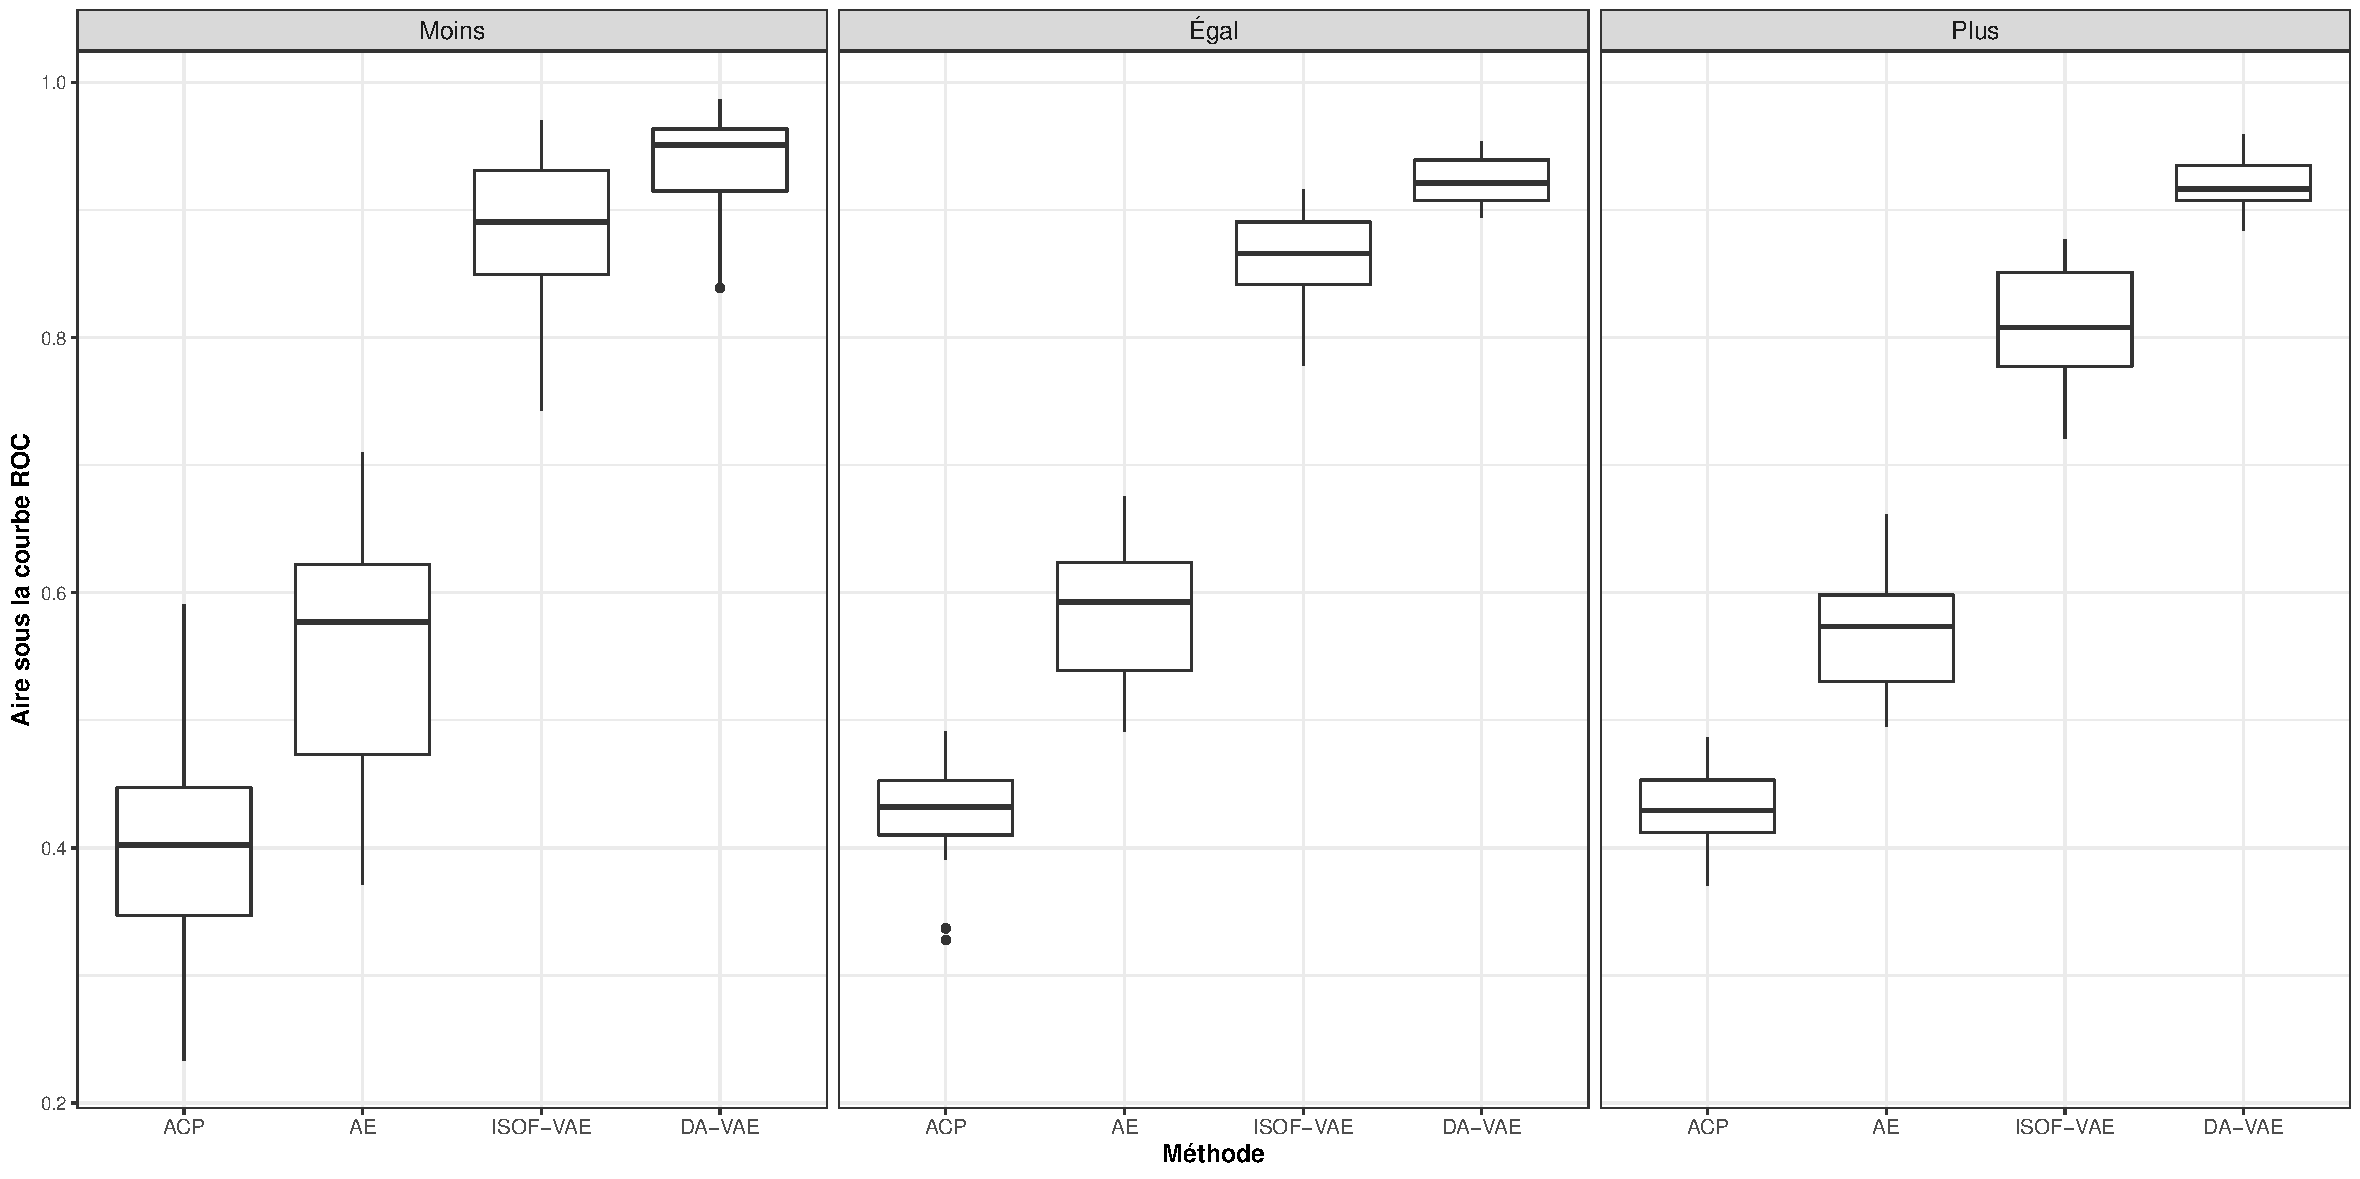
\includegraphics[width=12cm]{images/images_boxplots/auc_cars.pdf}
		\caption{Résultats en aire sous la courbe ROC}
	\end{subfigure}
	\begin{subfigure}{12cm}
		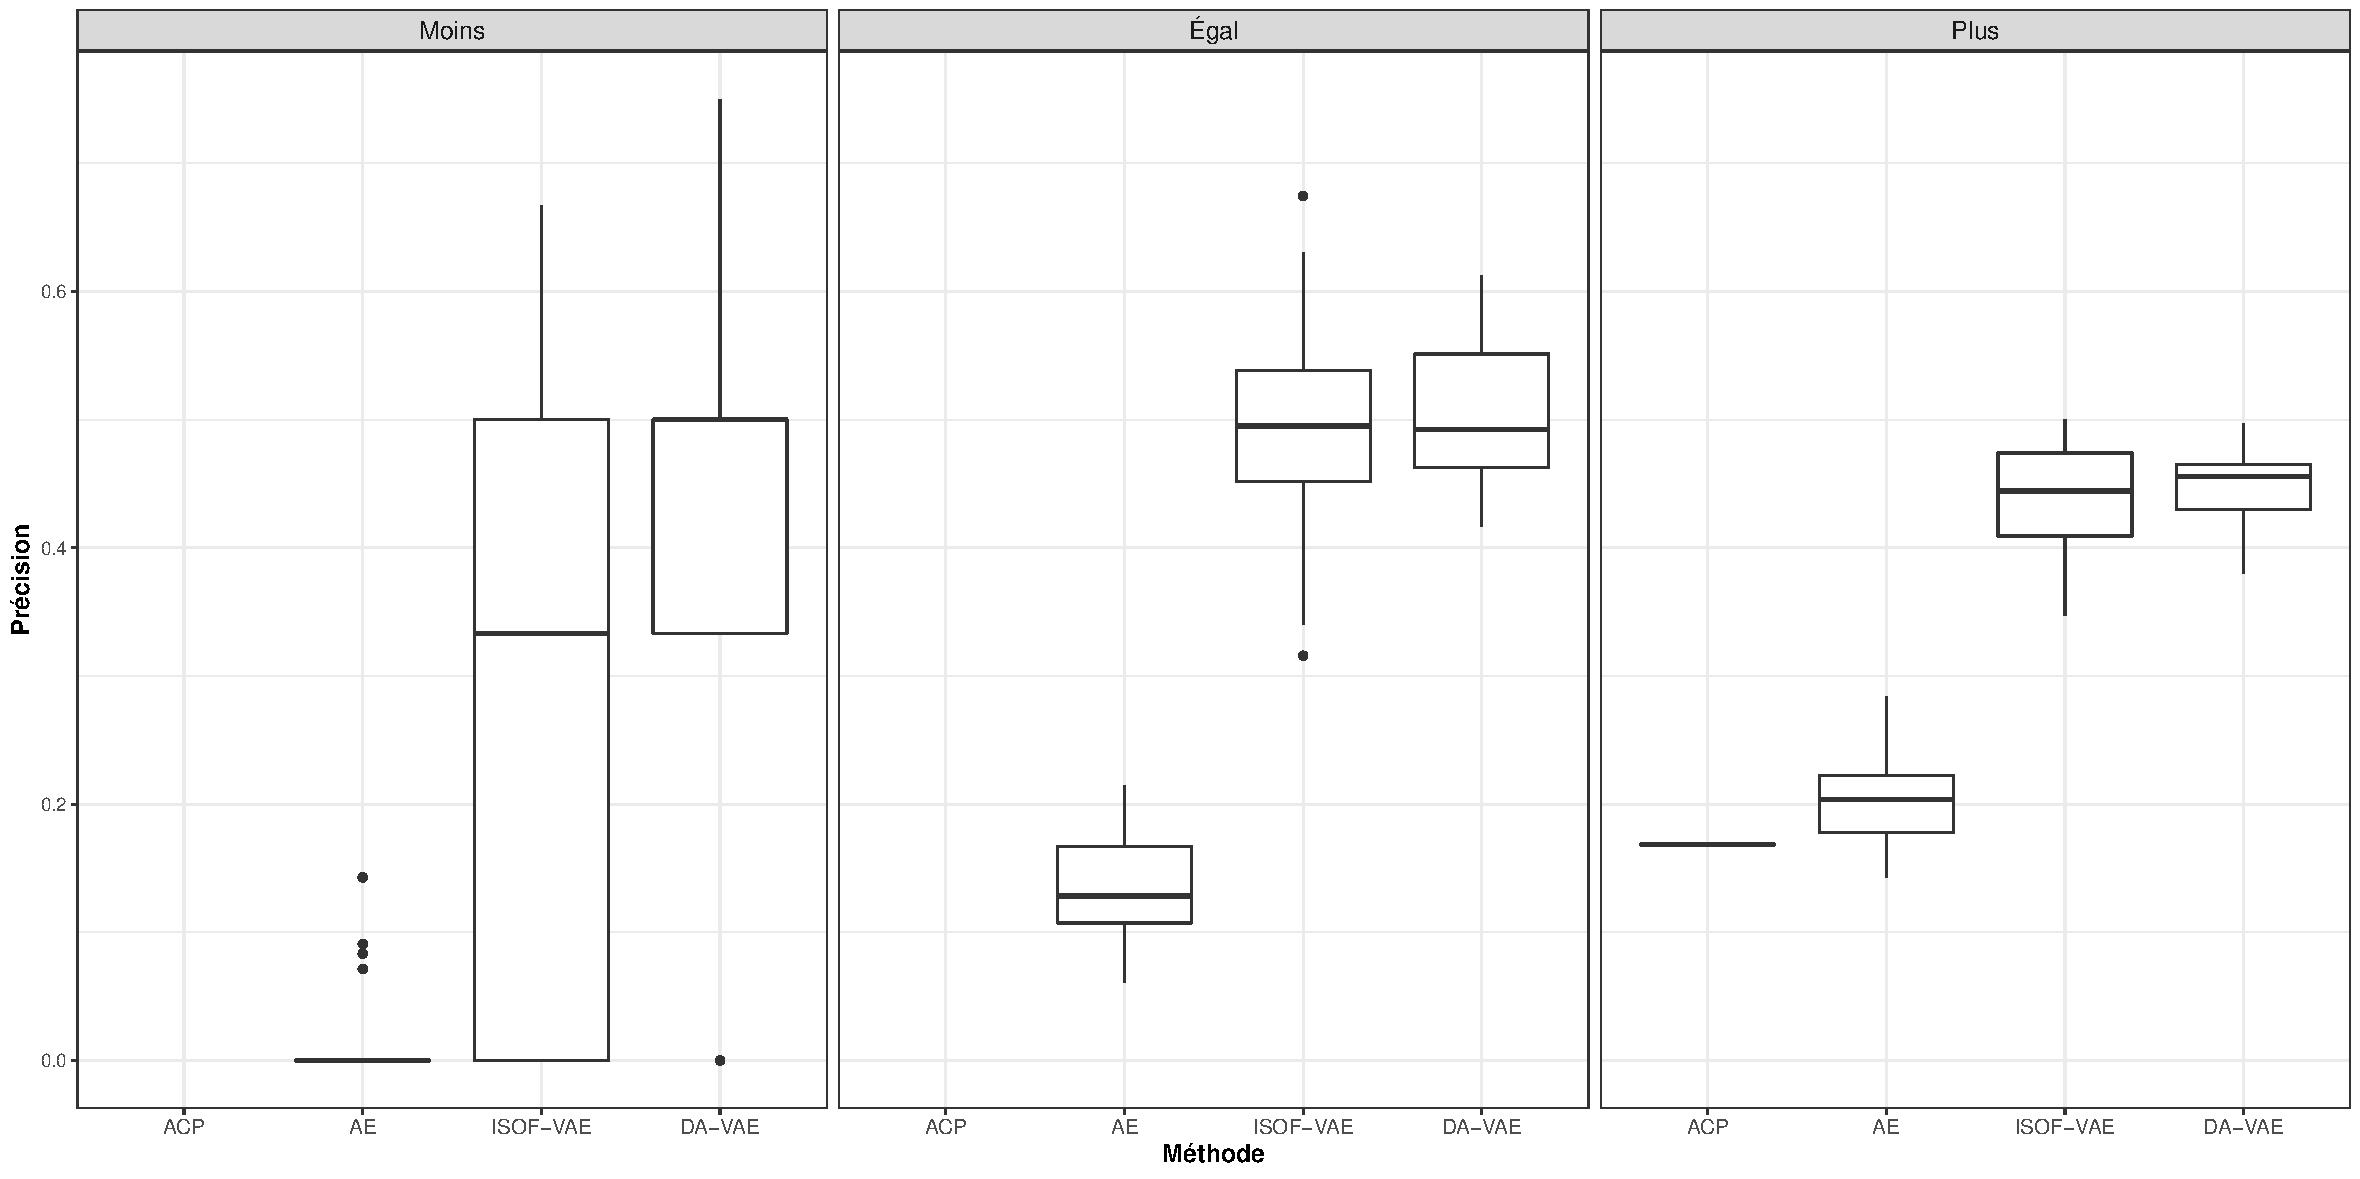
\includegraphics[width=12cm]{images/images_boxplots/precision_cars.pdf}
		\caption{Résultats en précision}
	\end{subfigure}
	\begin{subfigure}{12cm}
		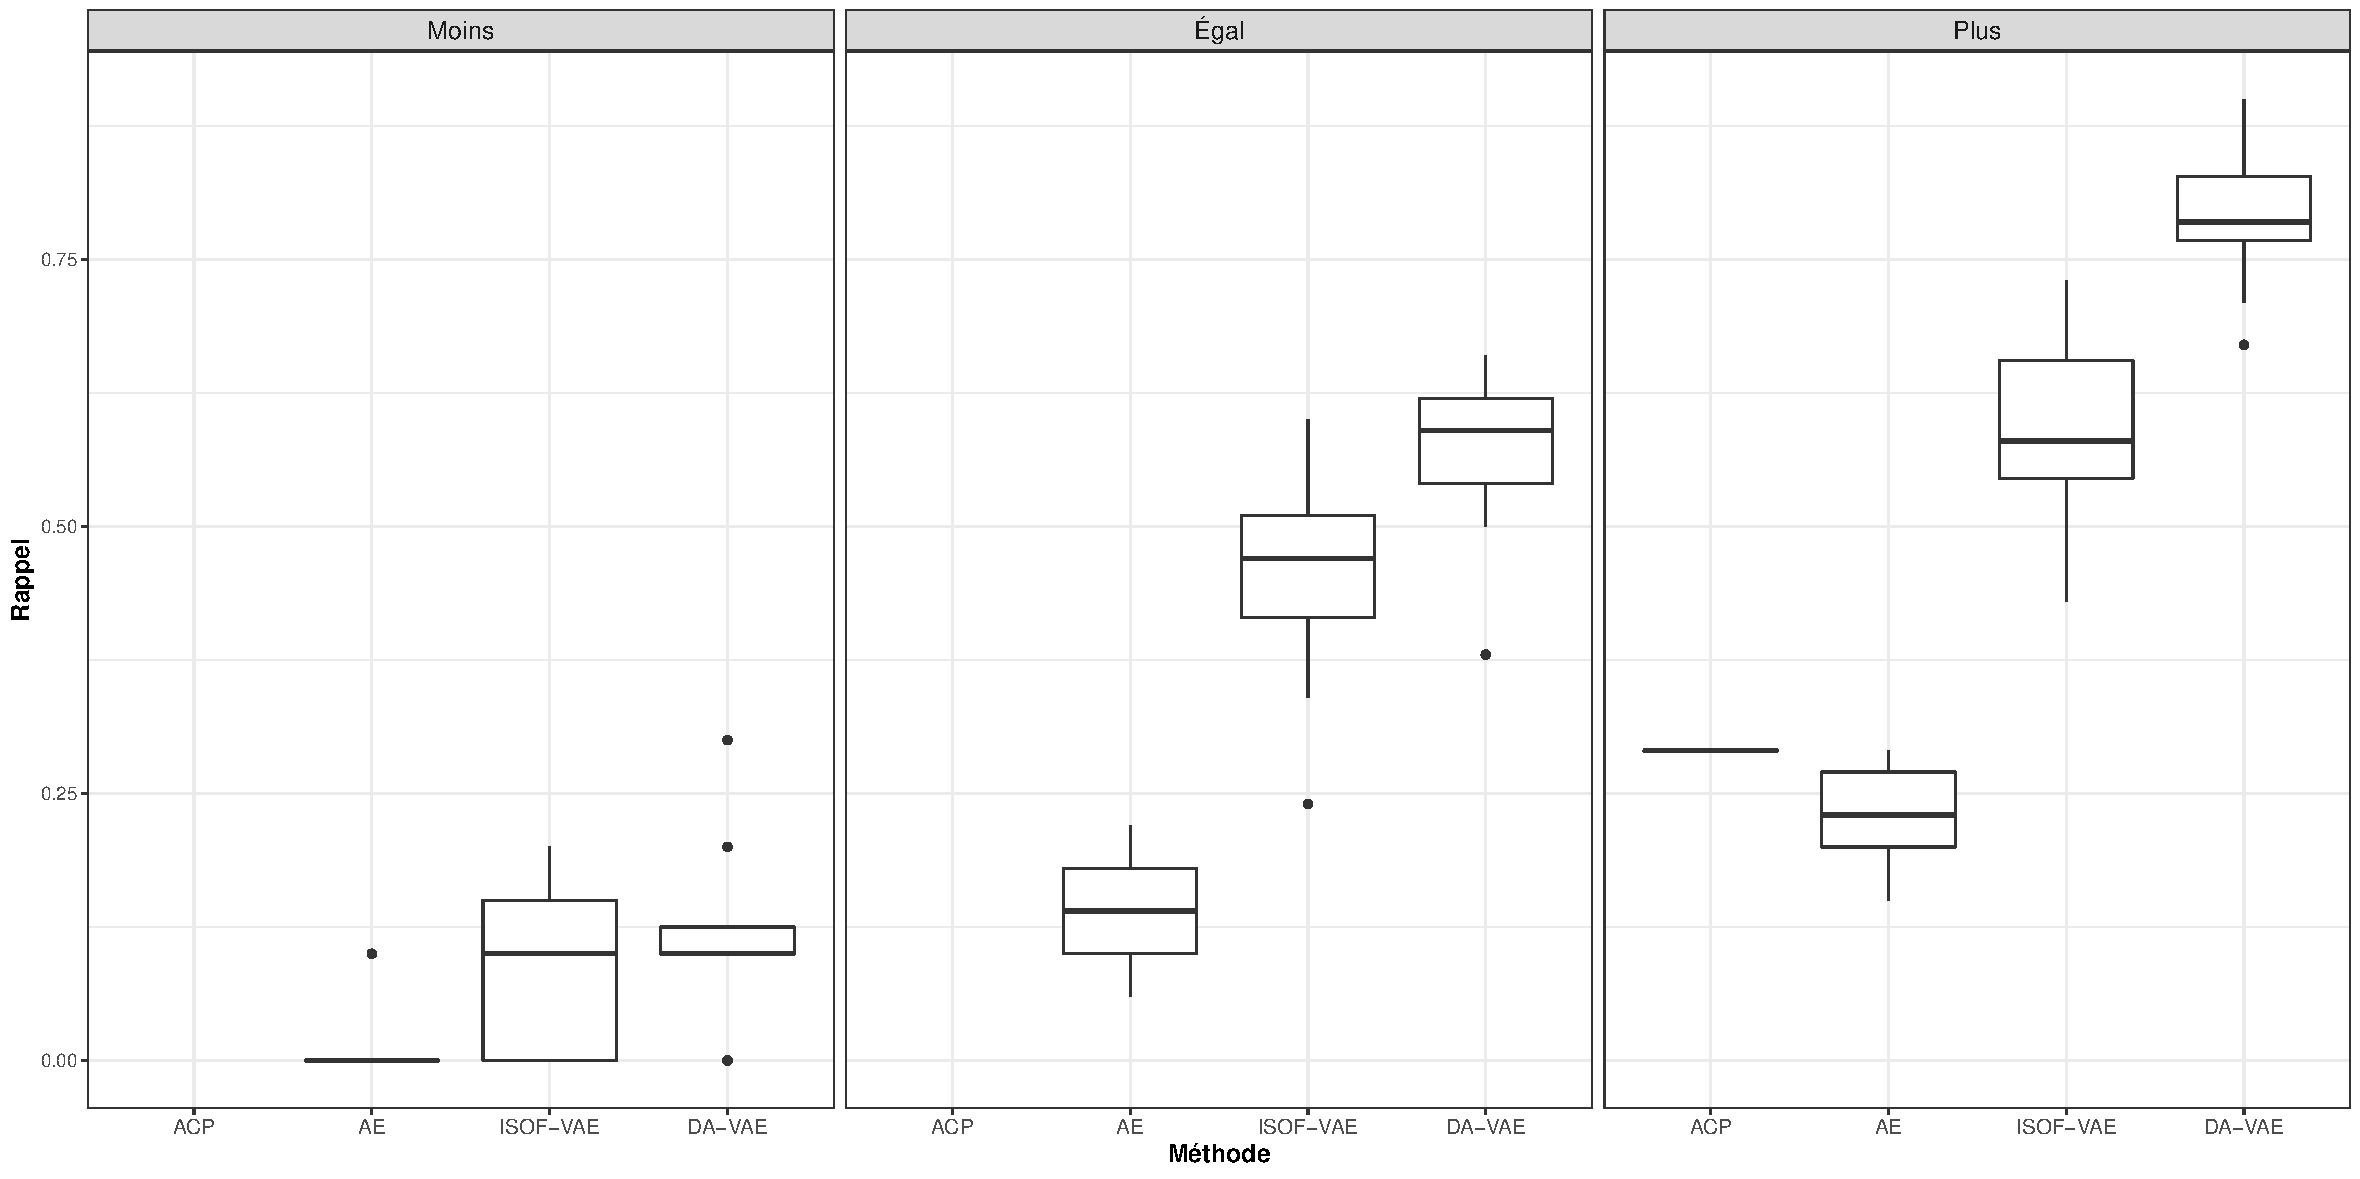
\includegraphics[width=12cm]{images/images_boxplots/recall_cars.pdf}
		\caption{Résultats en rappel}
	\end{subfigure}
	\caption{Graphiques en boîtes et moustaches illustrant les résultats sur les 20 réplications de chacune des approches et scénarios de contamination. Les \DIFdelbeginFL \DIFdelFL{3 }\DIFdelendFL \DIFaddbeginFL \DIFaddFL{trois }\DIFaddendFL sous-figures concernent une métrique différente.}
	\label{fig:auc_cars}
\end{figure}

\subsection{MNIST}

Le tableau \ref{tab:auc_mnist} synthétise les résultats obtenus sur le jeu de données \textit{MNIST} pour la métrique d'aire sous la courbe ROC. Les résultats sont présentés par scénario de contamination et par scénario de test (voir tableau \ref{tab:mnist_scenarios} pour plus de détails sur les scénarios de test). Les résultats pour les métriques de précision et de rappel sont présentés de la même manière dans les tableaux \ref{tab:precision_mnist} et \ref{tab:recall_mnist} respectivement. Nous avons mis en gras les méthodes qui sont significativement meilleures que toutes les autres. Nous avons utilisé le même test qu'expliqué à la sous-section \ref{results:imagenet}.

\begin{table}[h]
	\centering
	\caption{Résultats des aires sous la courbe ROC des différentes approches selon le scénario de contamination et le scénario de test appliqué sur le jeu de données \textit{MNIST} (moyennes sur les 20 réplications $\pm$ un écart-type).}
	\begin{tabular}{c|c|c c c c}
		\toprule
		Contamination & Scénario & ACP & AE & ISOF-VAE & DA-VAE \\
		\hline
		\multirow{6}{*}{Moins} 
		& 1 & $\mathbf{0.991 \pm 0.006}$ & 0.990 $\pm$ 0.004 & $0.969 \pm 0.031$ & 0.987 $\pm$ 0.007   \\
		& 2 & $0.988 \pm 0.005$ & $0.988 \pm 0.005$ & $0.965 \pm 0.022$ & 0.982 $\pm$ 0.021   \\
		& 3 & 0.993 $\pm$ 0.005 & $0.994 \pm 0.004$ & $0.976 \pm 0.017$ & 0.992 $\pm$ 0.005   \\
		& 4 & 0.893 $\pm$ 0.034 & $\mathbf{0.929 \pm 0.034}$ & $0.754 \pm 0.078$ & 0.836 $\pm$ 0.067   \\			
		& 5 & 0.893 $\pm$ 0.035 & $\mathbf{0.948 \pm 0.026}$ & $0.794 \pm 0.061$ & 0.880 $\pm$ 0.059   \\
		& 6 & 0.856 $\pm$ 0.059 & 0.847 $\pm$ 0.092 & $0.850 \pm 0.065$ & $\mathbf{0.893 \pm 0.046}$   \\
		\midrule
		\multirow{6}{*}{Égal} 
		& 1 & 0.993 $\pm$ 0.004 & $0.994 \pm 0.002$ & $0.980 \pm 0.011$ & $\mathbf{0.994 \pm 0.002}$   \\
		& 2 & 0.991 $\pm$ 0.003 & $0.992 \pm 0.002$ & $0.978 \pm 0.010$ & 0.988 $\pm$ 0.007   \\
		& 3 & 0.993 $\pm$ 0.004 & $\mathbf{0.996 \pm 0.001}$ & $0.980 \pm 0.011$ & 0.991 $\pm$ 0.007   \\
		& 4 & 0.903 $\pm$ 0.027 & $\mathbf{0.959 \pm 0.012}$ & $0.828 \pm 0.060$ & 0.901 $\pm$ 0.042   \\			
		& 5 & 0.913 $\pm$ 0.027 & $\mathbf{0.969 \pm 0.010}$ & $0.824 \pm 0.057$ & 0.871 $\pm$ 0.122   \\
		& 6 & 0.900 $\pm$ 0.031 & 0.854 $\pm$ 0.049 & $0.860 \pm 0.056$ & $\mathbf{0.921 \pm 0.036}$   \\
		\midrule
		\multirow{6}{*}{Plus} 
		& 1 & 0.994 $\pm$ 0.003 & $\mathbf{0.998 \pm 0.001}$ & $0.986 \pm 0.009$ & 0.994 $\pm$ 0.003   \\
		& 2 & 0.993 $\pm$ 0.004 & $\mathbf{0.997 \pm 0.001}$ & $0.981 \pm 0.009$ & 0.991 $\pm$ 0.007   \\
		& 3 & 0.993 $\pm$ 0.003 & $\mathbf{0.998 \pm 0.001}$ & $0.985 \pm 0.008$ & 0.995 $\pm$ 0.002   \\
		& 4 & 0.942 $\pm$ 0.025 & $\mathbf{0.985 \pm 0.005}$ & $0.833 \pm 0.058$ & 0.915 $\pm$ 0.041   \\			
		& 5 & 0.948 $\pm$ 0.021 & $\mathbf{0.992 \pm 0.003}$ & $0.875 \pm 0.040$ & 0.936 $\pm$ 0.028   \\
		& 6 & 0.929 $\pm$ 0.015 & 0.911 $\pm$ 0.027 & $0.882 \pm 0.031$ & $0.933 \pm 0.028$   \\
		\midrule
	\end{tabular} 
	\label{tab:auc_mnist}
\end{table}

Dans les figures \ref{fig:auc_mnist}, \ref{fig:precision_mnist} et \ref{fig:recall_mnist}, on peut voir plus en détails la distribution des résultats obtenus pour les \DIFdelbegin \DIFdel{3 }\DIFdelend \DIFaddbegin \DIFadd{trois }\DIFaddend différentes métriques sur les 20 réplications grâce à des graphiques en boîtes et moustaches.

\begin{figure}[H]
	\centering
	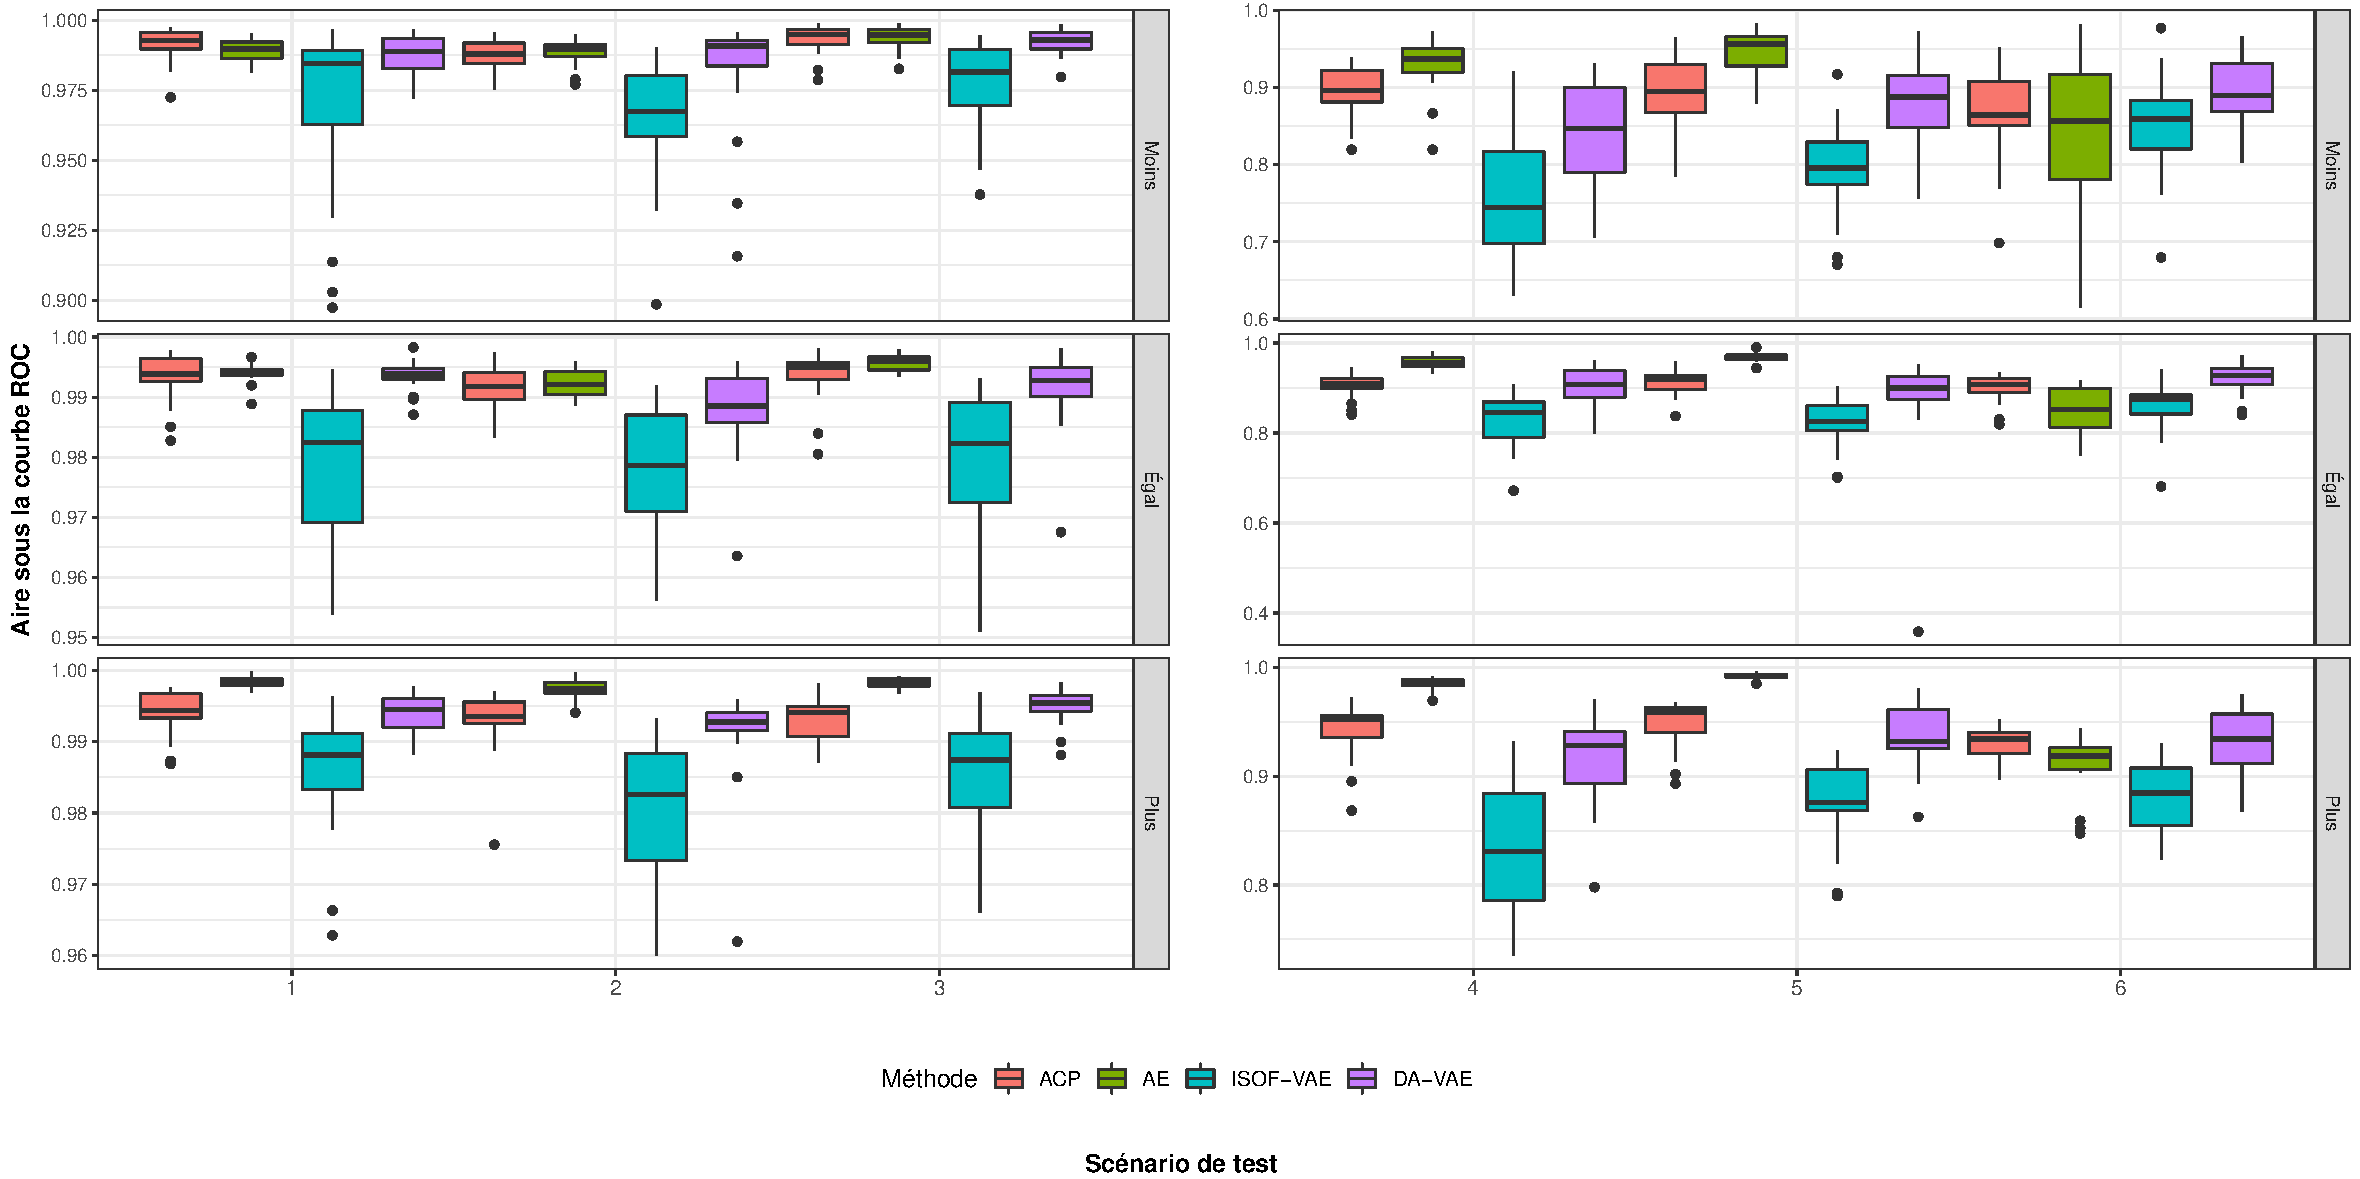
\includegraphics[width=\linewidth]{images/images_boxplots/auc_mnist.pdf}
	\caption{Graphiques en boîtes et moustaches illustrant les résultats sur les 20 réplications de chacune des approches, des scénarios de test et des scénarios de contamination. Toutes les figures présentent les résultats en aire sous la courbe ROC.}
	\label{fig:auc_mnist}
\end{figure}

\begin{table}[h]
	\centering
	\caption{Résultats des précisions selon la quantité de contamination et le scénario de test sur le jeu de données \textit{MNIST}. La valeur de $\alpha$ dépend du scénario de contamination. Pour le scénario "Moins" $\alpha=0.01$, pour le scénario "Égal" $\alpha=0.05$ et finalement pour le scénario "Plus" $\alpha=0.1$ (moyennes sur les 20 réplications $\pm$ un écart-type).}
	\begin{tabular}{c|c|c c c c }
		\toprule
		Contamination & Scénario & ACP & AE & ISOF-VAE & DA-VAE  \\
		\hline
		\multirow{6}{*}{Moins} 
		& 1 & $\mathbf{0.688 \pm 0.384}$ & 0.256 $\pm$ 0.097 & 0.280 $\pm$ 0.255 & 0.271 $\pm$ 0.212  \\
		& 2 & $0.500 \pm 0.424$ & 0.141 $\pm$ 0.178 & 0.238 $\pm$ 0.234 & 0.282 $\pm$ 0.243  \\
		& 3 & $\mathbf{0.583 \pm 0.482}$ & 0.411 $\pm$ 0.319 & 0.263 $\pm$ 0.289 & 0.387 $\pm$ 0.273  \\
		& 4 & 0.135 $\pm$ 0.182 & $0.197 \pm 0.193$ & 0.033 $\pm$ 0.057 & 0.020 $\pm$ 0.051  \\			
		& 5 & 0.110 $\pm$ 0.188 & $0.168 \pm 0.212$ & 0.028 $\pm$ 0.053 & 0.145 $\pm$ 0.159  \\
		& 6 & 0.118 $\pm$ 0.145 & $\mathbf{0.363 \pm 0.267}$ & 0.060 $\pm$ 0.092 & 0.115 $\pm$ 0.142  \\
		\midrule
		\multirow{6}{*}{Égal} 
		& 1 & 0.779 $\pm$ 0.079 & 0.777 $\pm$ 0.037 & 0.678 $\pm$ 0.102 & $0.809 \pm 0.057$  \\
		& 2 & $0.685 \pm 0.013$ & 0.672 $\pm$ 0.014 & 0.677 $\pm$ 0.011 & 0.681 $\pm$ 0.009  \\
		& 3 & 0.821 $\pm$ 0.056 & 0.793 $\pm$ 0.033 & 0.702 $\pm$ 0.089 & $0.829 \pm 0.059$  \\
		& 4 & 0.276 $\pm$ 0.078 & $\mathbf{0.526 \pm 0.063}$ & 0.216 $\pm$ 0.096 & 0.375 $\pm$ 0.108  \\			
		& 5 & 0.329 $\pm$ 0.081 & $\mathbf{0.556 \pm 0.050}$ & 0.210 $\pm$ 0.097 & 0.358 $\pm$ 0.104  \\
		& 6 & 0.331 $\pm$ 0.065 & $\mathbf{0.501 \pm 0.056}$ & 0.283 $\pm$ 0.094 & 0.443 $\pm$ 0.113  \\
		\midrule
		\multirow{6}{*}{Plus} 
		& 1 & 0.535 $\pm$ 0.016 & $0.563 \pm 0.020$ & 0.545 $\pm$ 0.021 & 0.555 $\pm$ 0.027  \\
		& 2 & $0.583 \pm 0.024$ & 0.566 $\pm$ 0.021 & 0.550 $\pm$ 0.036 & 0.556 $\pm$ 0.025  \\
		& 3 & 0.531 $\pm$ 0.025 & $\mathbf{0.571 \pm 0.016}$ & 0.540 $\pm$ 0.025 & 0.559 $\pm$ 0.018  \\
		& 4 & 0.455 $\pm$ 0.048 & $\mathbf{0.496 \pm 0.020}$ & 0.321 $\pm$ 0.083 & 0.424 $\pm$ 0.057  \\			
		& 5 & 0.452 $\pm$ 0.039 & $\mathbf{0.507 \pm 0.020}$ & 0.379 $\pm$ 0.061 & 0.452 $\pm$ 0.050  \\
		& 6 & 0.425 $\pm$ 0.023 & $0.464 \pm 0.022$ & 0.394 $\pm$ 0.044 & 0.456 $\pm$ 0.036  \\
		\midrule
	\end{tabular} 
	\label{tab:precision_mnist}
\end{table}

\begin{figure}[H]
	\centering
	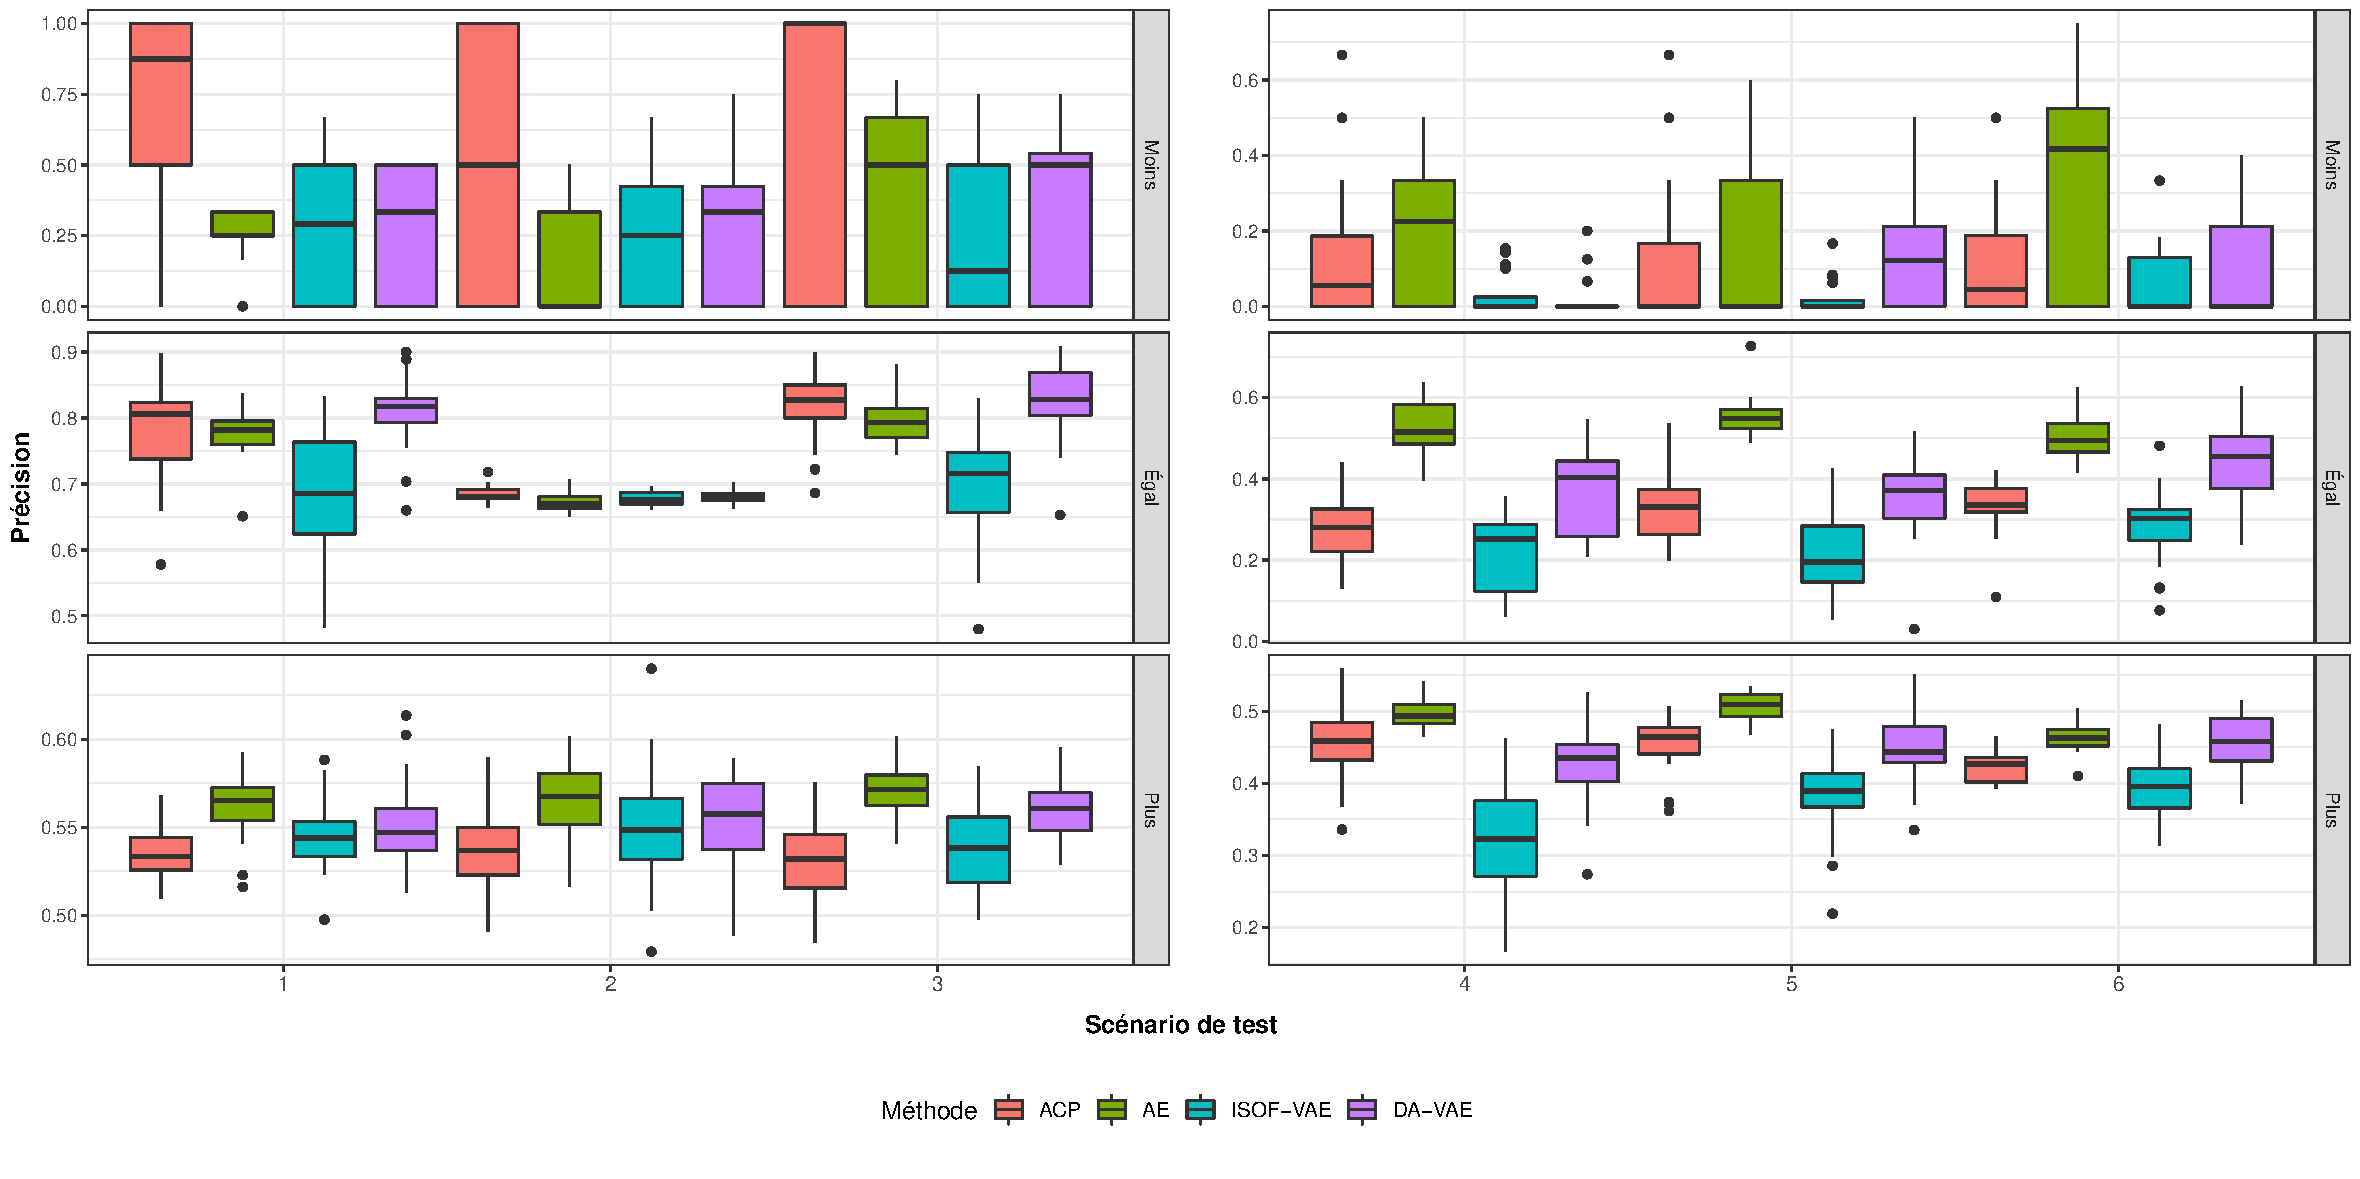
\includegraphics[width=\linewidth]{images/images_boxplots/precision_mnist.pdf}
	\caption{Graphiques en boîtes et moustaches illustrant les résultats sur les 20 réplications de chacune des approches, des scénarios de test et des scénarios de contamination. Toutes les figures présentent les résultats en précision.}
	\label{fig:precision_mnist}
\end{figure}

\begin{table}[h]
	\centering
	\caption{Résultats des rappels selon la quantité de contamination et le scénario de test sur le jeu de données \textit{MNIST}. La valeur de $\alpha$ dépend du scénario de contamination. Pour le scénario "Moins" $\alpha=0.01$, pour le scénario "Égal" $\alpha=0.05$ et finalement pour le scénario "Plus" $\alpha=0.1$ (moyennes sur les 20 réplications $\pm$ un écart-type).}
	\begin{tabular}{c|c|c c c c }
		\toprule
		Contamination & Scénario & ACP & AE & ISOF-VAE & DA-VAE  \\
		\hline
		\multirow{6}{*}{Moins} 
		& 1 & $0.200 \pm 0.139$ & 0.138 $\pm$ 0.067 & 0.095 $\pm$ 0.092 & 0.075 $\pm$ 0.062  \\
		& 2 & $0.100 \pm 0.085$ & 0.081 $\pm$ 0.107 & 0.085 $\pm$ 0.079 & 0.1 $\pm$ 0.095  \\
		& 3 & 0.131 $\pm$ 0.134 & $0.181 \pm 0.170$ & 0.09 $\pm$ 0.118 & 0.11 $\pm$ 0.094  \\
		& 4 & $0.100 \pm 0.116$ & 0.088 $\pm$ 0.089 & 0.038 $\pm$ 0.070 & 0.025 $\pm$ 0.063  \\			
		& 5 & 0.063 $\pm$ 0.093 & 0.075 $\pm$ 0.108 & 0.031 $\pm$ 0.054 & $0.088 \pm 0.089$  \\
		& 6 & 0.081 $\pm$ 0.099 & $\mathbf{0.156 \pm 0.130}$ & 0.056 $\pm$ 0.084 & 0.0625 $\pm$ 0.074  \\
		\midrule
		\multirow{6}{*}{Égal} 
		& 1 & 0.859 $\pm$ 0.083 & $0.871 \pm 0.067$ & 0.663 $\pm$ 0.110 & 0.778 $\pm$ 0.066  \\
		& 2 & $1.000 \pm 0.000$ & $1.000 \pm 0.000$ & 1.000 $\pm$ 0.001 & 1.000 $\pm$ 0.001  \\
		& 3 & 0.873 $\pm$ 0.079 & $0.901 \pm 0.038$ & 0.671 $\pm$ 0.116 & 0.786 $\pm$ 0.064  \\
		& 4 & 0.381 $\pm$ 0.096 & $\mathbf{0.628 \pm 0.090}$ & 0.239 $\pm$ 0.110 & 0.412 $\pm$ 0.123  \\			
		& 5 & 0.451 $\pm$ 0.123 & $\mathbf{0.645 \pm 0.079}$ & 0.230 $\pm$ 0.099 & 0.401 $\pm$ 0.112  \\
		& 6 & 0.435 $\pm$ 0.100 & $\mathbf{0.588 \pm 0.076}$ & 0.319 $\pm$ 0.101 & 0.481 $\pm$ 0.120  \\
		\midrule
		\multirow{6}{*}{Plus} 
		& 1 & 0.997 $\pm$ 0.005 & $\mathbf{1.000 \pm 0.000}$ & 0.980 $\pm$ 0.028 & 0.995 $\pm$ 0.007  \\
		& 2 & 0.994 $\pm$ 0.011 & $\mathbf{1.000 \pm 0.000}$ & 0.963 $\pm$ 0.031 & 0.985 $\pm$ 0.027  \\
		& 3 & 0.994 $\pm$ 0.008 & $\mathbf{1.000 \pm 0.000}$ & 0.977 $\pm$ 0.023 & 0.996 $\pm$ 0.010  \\
		& 4 & 0.841 $\pm$ 0.085 & $\mathbf{0.984 \pm 0.012}$ & 0.476 $\pm$ 0.159 & 0.733 $\pm$ 0.137  \\			
		& 5 & 0.873 $\pm$ 0.091 & $\mathbf{0.994 \pm 0.007}$ & 0.593 $\pm$ 0.139 & 0.824 $\pm$ 0.102  \\
		& 6 & 0.789 $\pm$ 0.055 & $\mathbf{0.859 \pm 0.047}$ & 0.629 $\pm$ 0.104 & 0.807 $\pm$ 0.097  \\
		\midrule
	\end{tabular} 
	\label{tab:recall_mnist}
\end{table}

\begin{figure}[H]
	\centering
	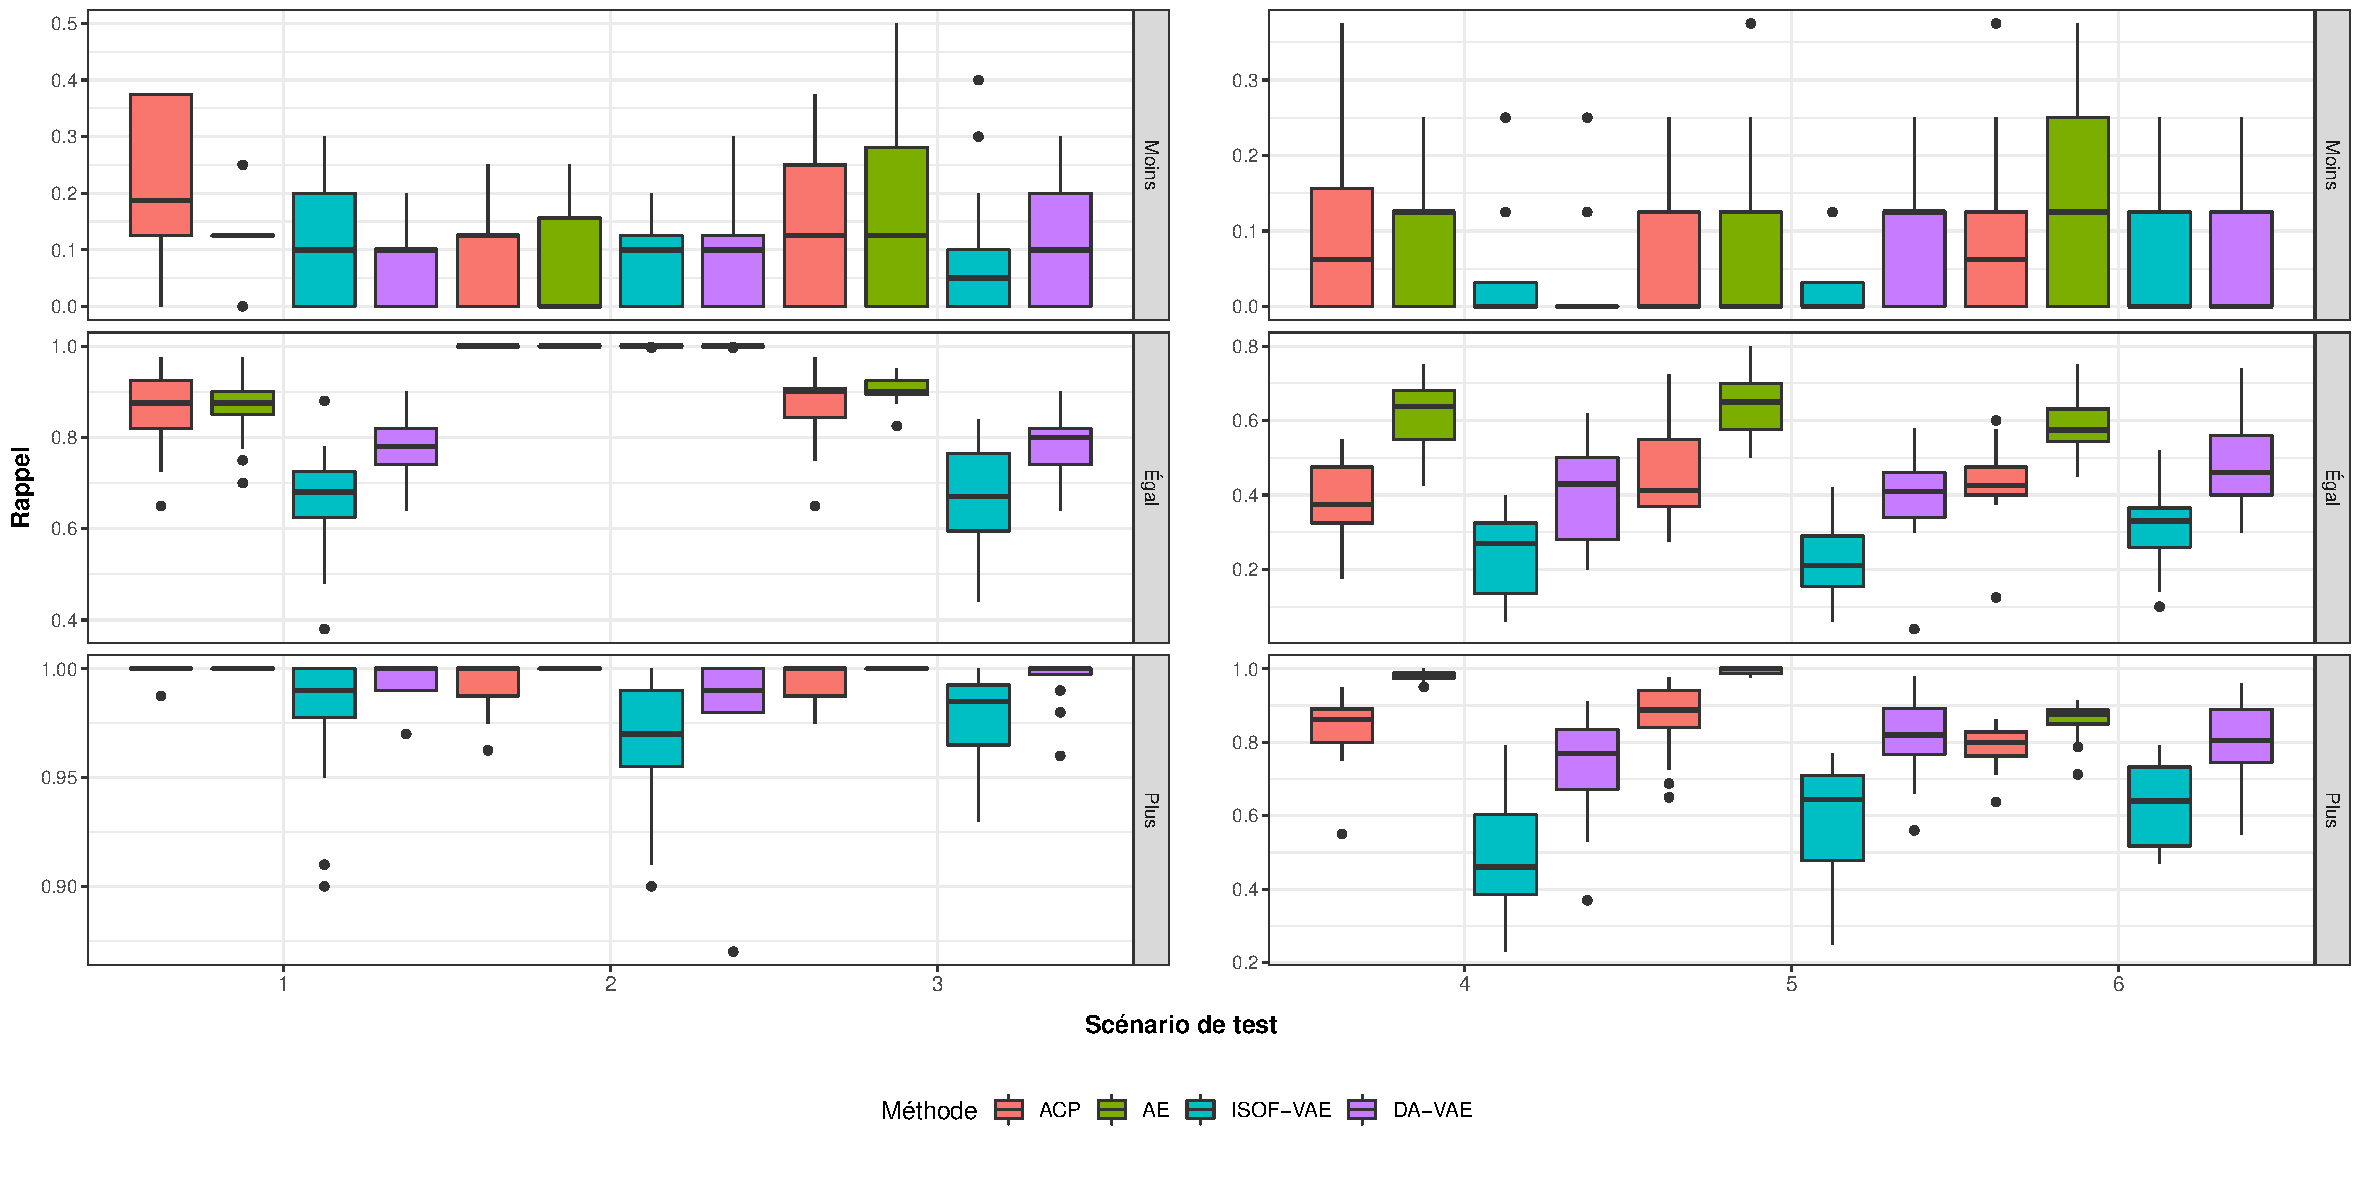
\includegraphics[width=\linewidth]{images/images_boxplots/recall_mnist.pdf}
	\caption{Graphiques en boîtes et moustaches illustrant les résultats sur les 20 réplications de chacune des approches, des scénarios de test et des scénarios de contamination. Toutes les figures présentent les résultats en rappel.}
	\label{fig:recall_mnist}
\end{figure}

\subsection{Discussion et interprétation des résultats} \label{discussion}

Dans les prochaines sous-sections, nous discuterons des résultats obtenus par les différentes méthodes sur les deux jeux de données. Nous irons également plus en profondeur dans l'analyse de la méthode DA-VAE en regardant le comportement de la perte en entraînement ainsi que la composition des représentations latentes produites par le modèle. Finalement, nous étudierons l'impact du niveau de contamination sur les résultats et la pertinence du niveau de filtration $\alpha$.

\subsection{Résultats sur \textit{ImageNet}} \label{imagenet_results}

Dans le tableau \ref{tab:results_cars}, on peut voir les performances en aire sous la courbe ROC, en précision et en rappel de chacune des approches. Pour les 3 scénarios de contamination différents, on remarque que \DIFdelbegin \DIFdel{2 }\DIFdelend \DIFaddbegin \DIFadd{deux }\DIFaddend méthodes sont beaucoup plus performantes, et ce, pour les \DIFdelbegin \DIFdel{3 }\DIFdelend \DIFaddbegin \DIFadd{trois }\DIFaddend métriques. Ces \DIFdelbegin \DIFdel{2 }\DIFdelend \DIFaddbegin \DIFadd{deux }\DIFaddend approches sont: ISOF-VAE et DA-VAE. Il est intéressant de remarquer que ces \DIFdelbegin \DIFdel{2 }\DIFdelend \DIFaddbegin \DIFadd{deux }\DIFaddend approches utilisent la représentation latente de l'image pour discriminer les anomalies des observations "normales" plutôt que la reconstruction faite sur les dimensions originales de l'image. Dans la sous-section \ref{imagenet:reconsruction}, nous ferons l'analyse plus en profondeur des résultats moins performants des méthodes basées sur la reconstruction.

Notre approche DA-VAE est celle qui est la plus performante selon les métriques moyennes analysées. En tenant compte du test de Mann-Whitney, nous sommes en mesure de conclure que la méthode DA-VAE est même significativement supérieure à ISOF-VAE en aire sous la courbe ROC, et ce, pour les \DIFdelbegin \DIFdel{3 }\DIFdelend \DIFaddbegin \DIFadd{trois }\DIFaddend scénarios de contamination. Pour ce qui est des résultats en précision, les deux méthodes ne sont pas significativement différentes. Pour la métrique de rappel, la méthode DA-VAE est significativement supérieure dans \DIFdelbegin \DIFdel{2 des 3 }\DIFdelend \DIFaddbegin \DIFadd{deux des trois }\DIFaddend scénarios de contamination. On remarque également  que les performances en aire sous la courbe ROC de la méthode DA-VAE demeurent élevées, et ce, pour les \DIFdelbegin \DIFdel{3 }\DIFdelend \DIFaddbegin \DIFadd{trois }\DIFaddend scénarios de contamination. Dans le cas de ISOF-VAE, les performances moyennes en aire sous la courbe ROC passent de 0.886 pour le scénario "Moins" à 0.811 pour le scénario "Plus". La variabilité des résultats de notre approche DA-VAE est également inférieure à celle obtenue sur ISOF-VAE pour les trois métriques. En analysant davantage les résultats sur les trois différents scénarios de contamination, on peut remarquer que pour toutes les approches, le scénario de contamination "Moins" est celui qui témoigne de la plus grande volatilité dans ses performances en test. Cela était prévisible sachant qu'il n'y a que très peu d'anomalies, soit $1\%$, dans le jeu de données de test. Dans les \DIFdelbegin \DIFdel{3 }\DIFdelend \DIFaddbegin \DIFadd{trois }\DIFaddend sous-figures de la figure \ref{fig:pvalues_scenarios}, on peut voir les scores d'anomalie prédits pour chacune des observations du jeu de données test en fonction de si l'observation est "anormale" ou non, et ce, pour les 3 scénarios de contamination. Chacun des points correspond à une observation. Les observations sont ordonnées en ordre croissant selon l'inverse de leur score d'anomalie, soit $1-\gamma$. Ce score d'anomalie est défini à l'équation \ref{eq:score_anomalie}. \DIFdelbegin \DIFdel{Entre }\DIFdelend \DIFaddbegin \DIFadd{En }\DIFaddend d'autres mots, plus une observation est située à gauche sur l'axe des $x$, plus elle est "anormale" selon le modèle DA-VAE. Les points de couleur violette sont des observations que nous connaissons comme "normales" alors que les points jaunes sont des observations que nous connaissons comme "anormales". Le trait horizontal rouge correspond à la valeur de notre niveau de filtration $\alpha$. Avec ce niveau de filtration, les observations sous la droite rouge sont considérées "anormales" alors que celles au-dessus sont considérées comme "normales" selon le modèle. La ligne verte correspond simplement à un trait partant de l'origine $(0,0)$ et allant jusqu'au point $(1,1)$. Cette ligne nous servira de point de référence pour comparer différents scénarios de contamination. Pour chaque sous-figure, nous présentons une vue complète des observations du jeu de données de test ainsi qu'une vue rapprochée sur les observations situées plus à gauche de l'axe des $x$.

\begin{figure}[htb]
	\centering
	\begin{subfigure}{6cm}
		\centering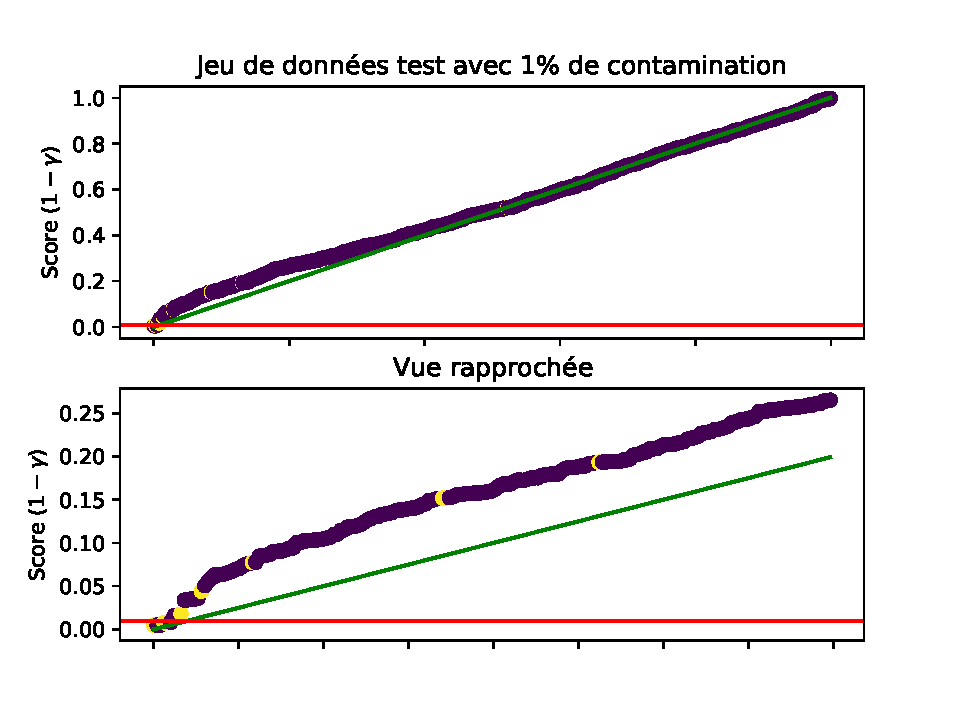
\includegraphics[width=6cm]{images/images_davae/pvalues_scenario_cars_moins}
		\caption{Scénario "Moins"}
	\end{subfigure}
	\begin{subfigure}{6cm}
		\centering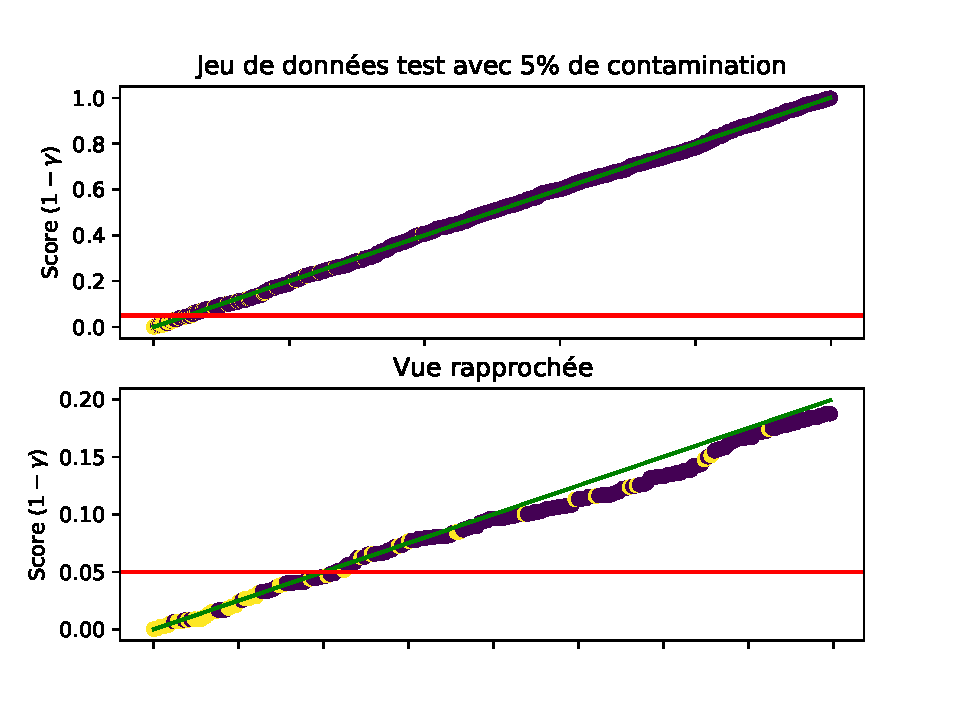
\includegraphics[width=6cm]{images/images_davae/pvalues_scenario_cars_egal}
		\caption{Scénario "Égal"}
	\end{subfigure}
	\begin{subfigure}{6cm}
		\centering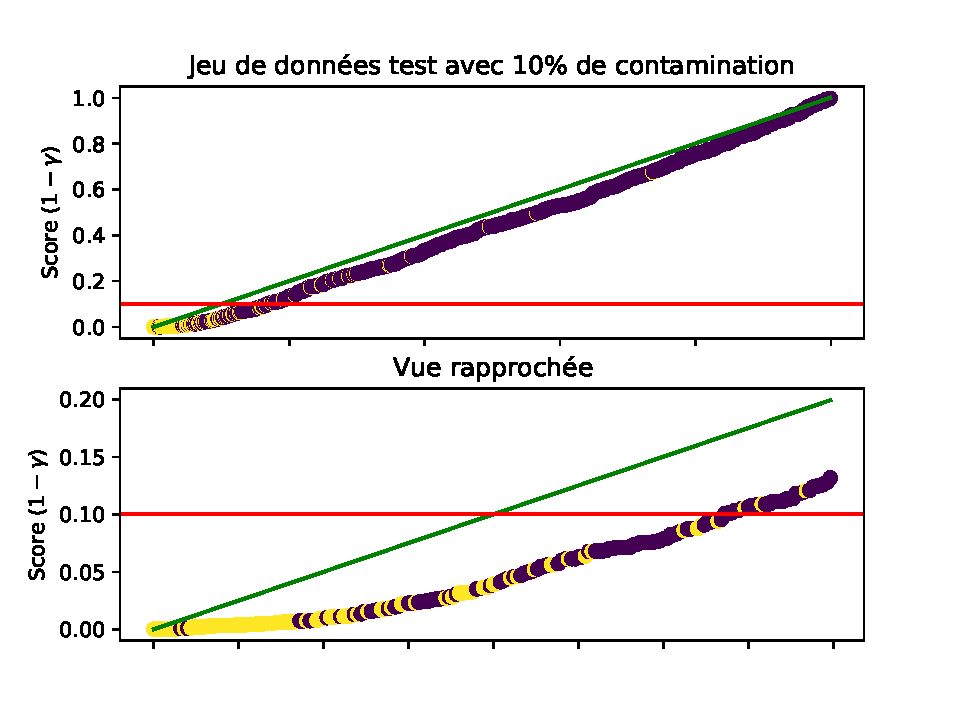
\includegraphics[width=6cm]{images/images_davae/pvalues_scenario_cars_plus}
		\caption{Scénario "Plus"}
	\end{subfigure}
	\caption{Graphiques illustrant les scores d'anomalies selon le scénario de contamination pour le modèle DA-VAE appliqué sur le jeu de données \textit{ImageNet}. Les points violets sont des observations que nous connaissons comme "normales" alors que les points jaunes sont des observations que nous connaissons comme "anormales". Dans tous les cas, le niveau de filtration $\alpha$ est défini comme le niveau de contamination dans le jeu de données de test. Pour chaque sous-figure, nous présentons une vue complète des observations du jeu de données de test ainsi qu'une vue rapprochée sur les observations situées plus à gauche de l'axe des $x$.} 
	\label{fig:pvalues_scenarios}
\end{figure}

Dans les \DIFdelbegin \DIFdel{3 }\DIFdelend \DIFaddbegin \DIFadd{trois }\DIFaddend sous-figures à la figure \ref{fig:pvalues_scenarios}, on peut voir que les observations "anormales", soit les points jaunes, sont principalement regroupées à gauche de l'axe des $x$, ce qui est le comportement souhaité. De plus, on peut remarquer que dans les \DIFdelbegin \DIFdel{3 }\DIFdelend \DIFaddbegin \DIFadd{trois }\DIFaddend différents scénarios, les points les plus \DIFdelbegin \DIFdel{gauches }\DIFdelend \DIFaddbegin \DIFadd{à gauche }\DIFaddend ne se retrouvent pas à la même position par rapport à la droite verte. Dans le scénario "Égal", l'ensemble des points est relativement bien aligné avec la courbe verte. Cette observation peut s'expliquer par le fait que les deux ensembles de données, $\mathcal{X}$ et $\mathcal{X^*}$, possèdent la même composition en termes de proportion d'anomalies. Dans le scénario "Moins", on peut observer une masse plus importante de points au-dessus de la courbe verte dans les premières observations. Cela est dû au fait que l'ensemble de test possède moins d'anomalies que l'ensemble d'entraînement, ce qui fait en sorte que davantage d'observations obtiennent des scores d'anomalie plus faibles. Finalement, dans le scénario "Plus", on observe qu'une masse de points se situent sous la courbe verte dans les premières observations. À l'inverse du scénario "Moins", l'ensemble de test possède ici davantage d'anomalies, en proportion, que l'ensemble d'entraînement, ce qui fait en sorte que davantage d'observations obtiennent des scores d'anomalies \DIFdelbegin \DIFdel{élevées}\DIFdelend \DIFaddbegin \DIFadd{élevés}\DIFaddend . Cette analyse nous permet de valider visuellement que l'approche s'adapte bien à différentes proportions de contamination dans les jeux de données de test et d'entraînement.

\subsubsection{Analyses des méthodes basées sur la reconstruction} \label{imagenet:reconsruction}

Dans la sous-section précédente, nous avons mentionné que les approches basées sur la reconstruction, soit ACP et AE, sont beaucoup moins performantes que les deux autres approches. D'ailleurs, on remarque que la méthode ACP obtient des aires sous la courbe ROC sous 0.5 pour tous les scénarios de contamination. En théorie, nous aurions donc pu, pour cette méthode, obtenir de meilleurs résultats en calculant notre score d'anomalie comme l'inverse du score actuel. Actuellement, notre prémisse de base est que les images étant les moins bien reconstruites sont potentiellement des anomalies. À l'inverse, les images les mieux reconstruites sont potentiellement des images "normales". Nous avons fait cette hypothèse puisque les anomalies sont peu fréquentes dans nos jeux de données, ce qui devrait faire en sorte que les paramètres appris par le modèle soient davantage représentés par les images "normales". En analysant les résultats en aire sous la courbe ROC obtenus par l'ACP, nous concluons que c'est plutôt les anomalies qui sont mieux reconstruites que les images "normales". Pour s'en convaincre, nous avons regardé des exemples d'images les mieux reconstruites sur l'ensemble d'entraînement. On peut voir quelques exemples à la figure \ref{fig:acp_reconstructionsa}. Dans le même ordre d'idées, la figure \ref{fig:acp_reconstructionsb} illustre quelques exemples d'images qui sont moins bien reconstruites. 

\begin{figure}[H]
	\centering
	\begin{subfigure}{12cm}
		\centering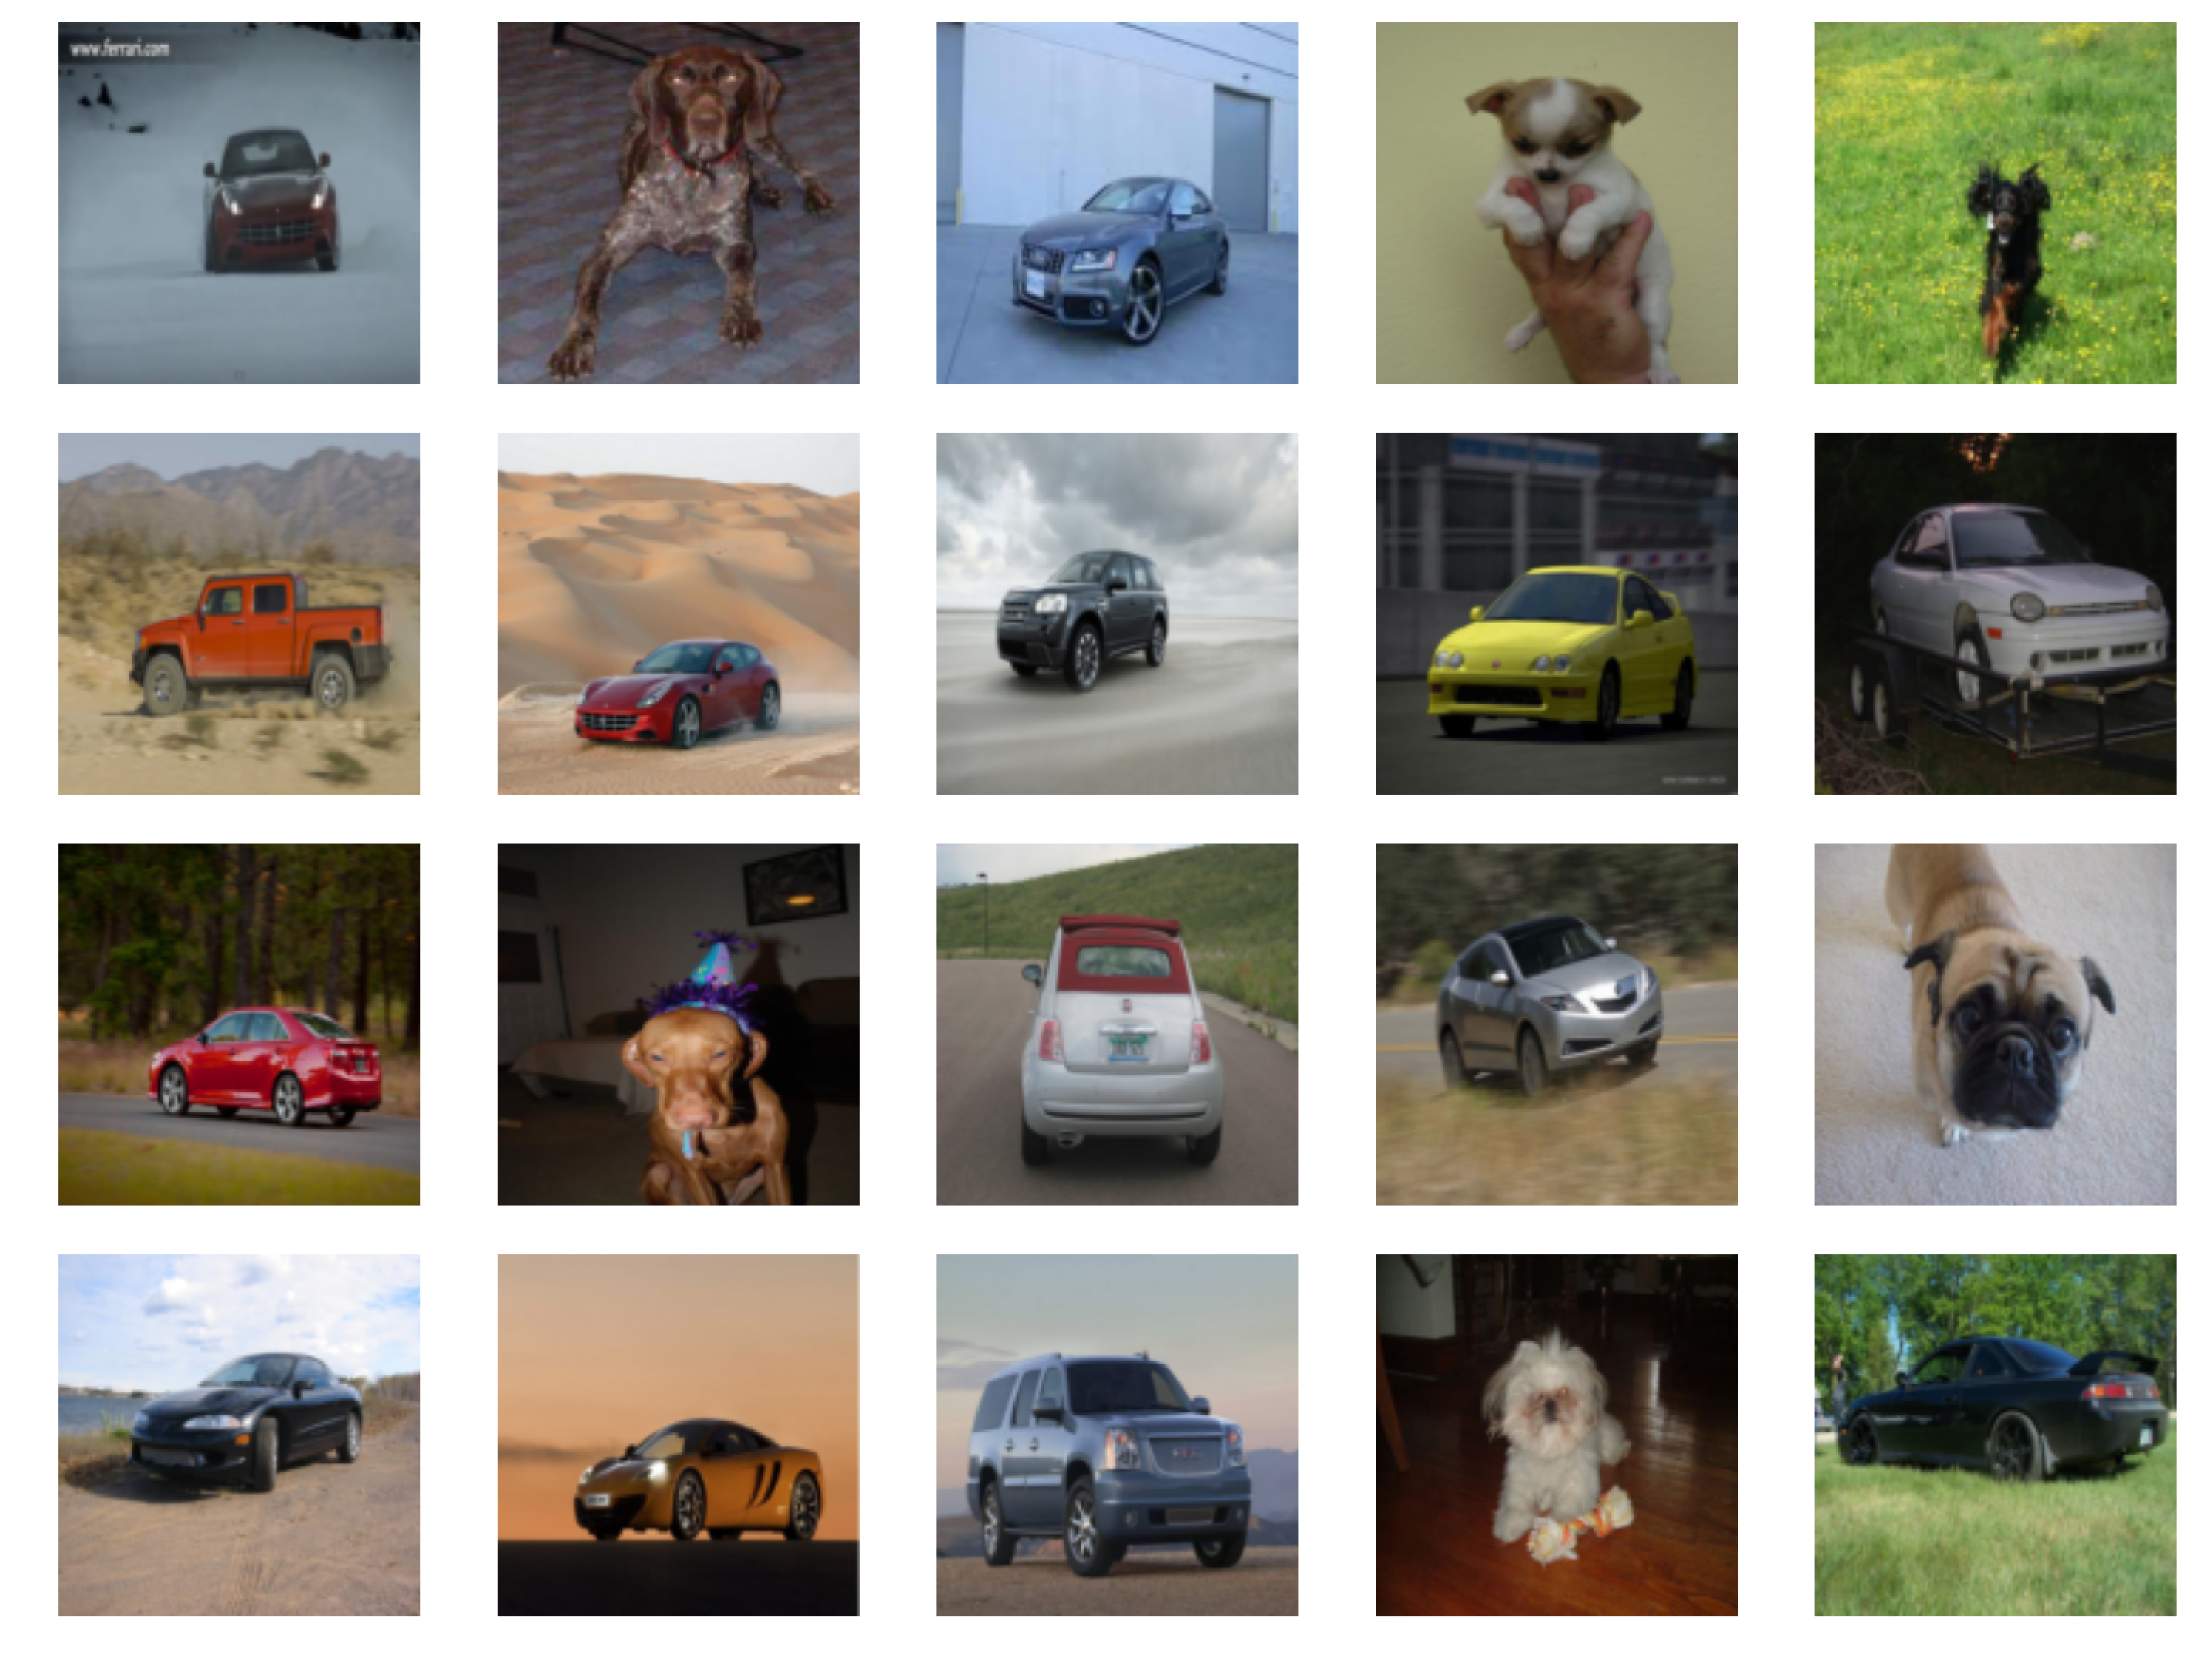
\includegraphics[width=12cm]{images/smallest_errors}
		\caption{Exemples d'images bien reconstruites}
		\label{fig:acp_reconstructionsa}
	\end{subfigure}
	\begin{subfigure}{12cm}
		\centering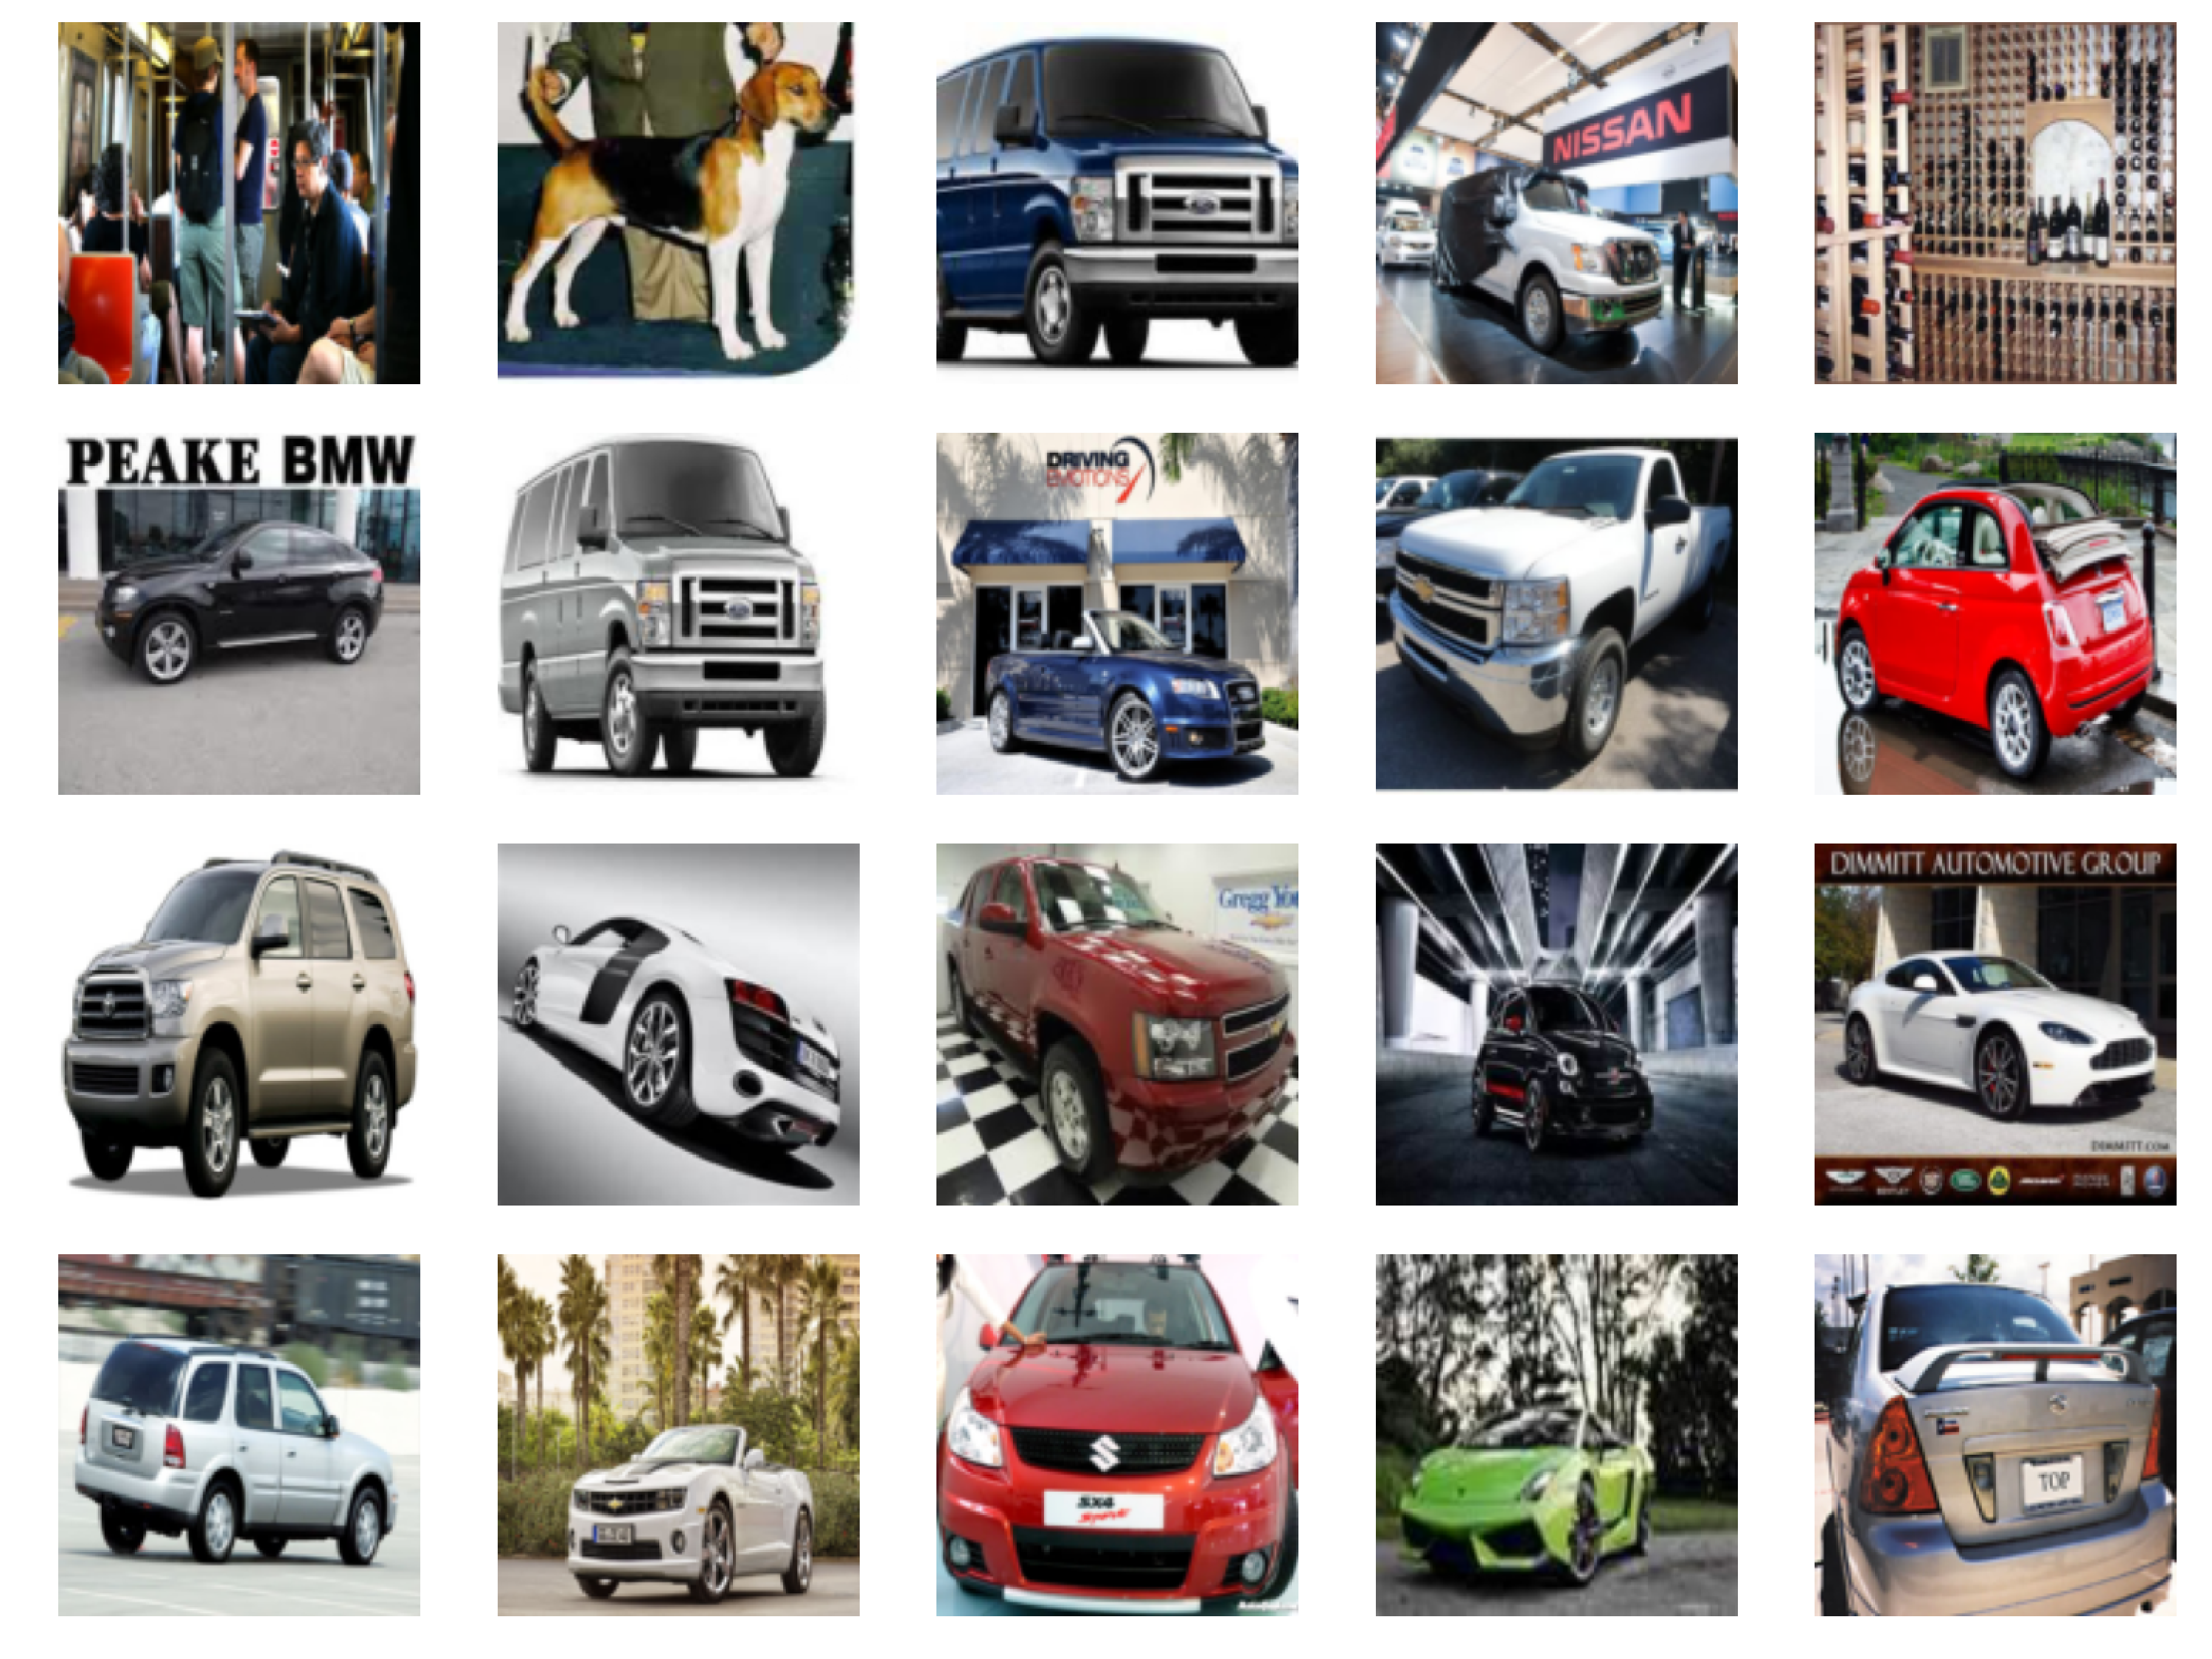
\includegraphics[width=12cm]{images/biggest_errors}
		\caption{Exemples d'images mal reconstruites}
		\label{fig:acp_reconstructionsb}
	\end{subfigure}
	\caption{Exemples d'images qui sont bien reconstruites (a) et mal reconstruites (b) selon la méthode ACP appliquée sur le jeu de données d'entraînement de \textit{ImageNet}.}
	\label{fig:acp_reconstructions}
\end{figure}

En analysant la figure \ref{fig:acp_reconstructions}, on remarque que les images bien reconstruites sont des images relativement "simples". \DIFdelbegin \DIFdel{Les imagesde la classe "normale" }\DIFdelend \DIFaddbegin \DIFadd{Ces images, que l'on peut voir }\DIFaddend à la figure \ref{fig:acp_reconstructionsa}\DIFaddbegin \DIFadd{, }\DIFaddend montrent des voitures avec une vue relativement éloignée. Les \DIFdelbegin \DIFdel{arrières plans }\DIFdelend \DIFaddbegin \DIFadd{arrière-plans }\DIFaddend sont également plutôt simples, avec des couleurs assez unies. À l'inverse, les images les moins biens reconstruites (figure \ref{fig:acp_reconstructionsb}) sont plus "complexes". Par exemple, on voit les voitures de très près, avec beaucoup de détails. Aussi, les \DIFdelbegin \DIFdel{arrières plans }\DIFdelend \DIFaddbegin \DIFadd{arrière-plans }\DIFaddend sont beaucoup plus complexes, avec différentes couleurs et formes. Au final, on pourrait conclure que la méthode basée sur l'ACP discrimine sur la complexité de l'image plutôt que sur le contenu (voitures versus autres). La méthode AE performe un peu mieux que l'ACP, mais elle obtient tout de même des aires sous la courbe ROC inférieures à 0.6, et ce, pour les \DIFdelbegin \DIFdel{3 }\DIFdelend \DIFaddbegin \DIFadd{trois }\DIFaddend scénarios de contamination. On pourrait penser que l'autoencodeur, avec la perte orientée sur le contenu\DIFaddbegin \DIFadd{, }\DIFaddend \textit{perceptual loss}, gère un peu mieux ces différents éléments (vues, couleurs, arrière-plan, etc), mais cela n'est pas suffisant pour obtenir des performances optimales. Au final, les méthodes basées sur l'erreur de reconstruction nous apparaissent moins pertinentes lorsque nous devons faire la détection d'anomalies dans des images de complexités et de styles différents.


\subsubsection{Analyse des représentations latentes} \label{analyse_lat_cars}

Dans la section \ref{cadre_decisionnel}, nous avons mentionné qu'il fallait analyser les statistiques de distance afin de savoir si une statistique de distance élevée est signe d'anomalie ou de \DIFaddbegin \DIFadd{"}\DIFaddend normalité\DIFaddbegin \DIFadd{"}\DIFaddend . Pour ce faire, il suffit de visualiser un échantillon d'images de notre jeu de données d'entraînement ayant des statistiques de distance élevées et un autre échantillon d'images ayant des statistiques de distance faibles. Dans la figure \ref{fig:latentes_images}, on peut voir quelques exemples provenant de ces échantillons. On remarque assez rapidement que les observations ayant des statistiques de distance faibles proviennent de notre classe "anormale". À l'inverse, les observations ayant des statistiques de distance élevées proviennent de notre classe "normale", soit des images de voitures. On remarque que les voitures de la figure \ref{fig:latentes_images} sont presque toutes des voitures rouges. Il est possible que les représentations latentes \DIFaddbegin \DIFadd{de }\DIFaddend ce type de voitures soient situées dans un espace similaire et le plus éloigné de la \DIFdelbegin \DIFdel{$N(0,1)$}\DIFdelend \DIFaddbegin \DIFadd{$N(0,I)$}\DIFaddend . Nous avons voulu valider si la couleur de la voiture avait un impact significatif dans la prise de décision. Pour ce faire, nous avons pré-sélectionné un échantillon d'images de voitures de différentes couleurs et avons calculé le score d'anomalie pour ces images. À la figure \ref{fig:random_samples}, on peut voir que les voitures rouges obtiennent des scores d'anomalie plutôt élevés, même une avec un score sous la valeur du seuil de filtration $\alpha$. Cela nous permet de confirmer que ce n'est pas \DIFaddbegin \DIFadd{que }\DIFaddend la couleur de la voiture \DIFdelbegin \DIFdel{seulement }\DIFdelend qui a un impact.

\begin{figure}[htb]
	\centering
	\begin{subfigure}{6cm}
		\centering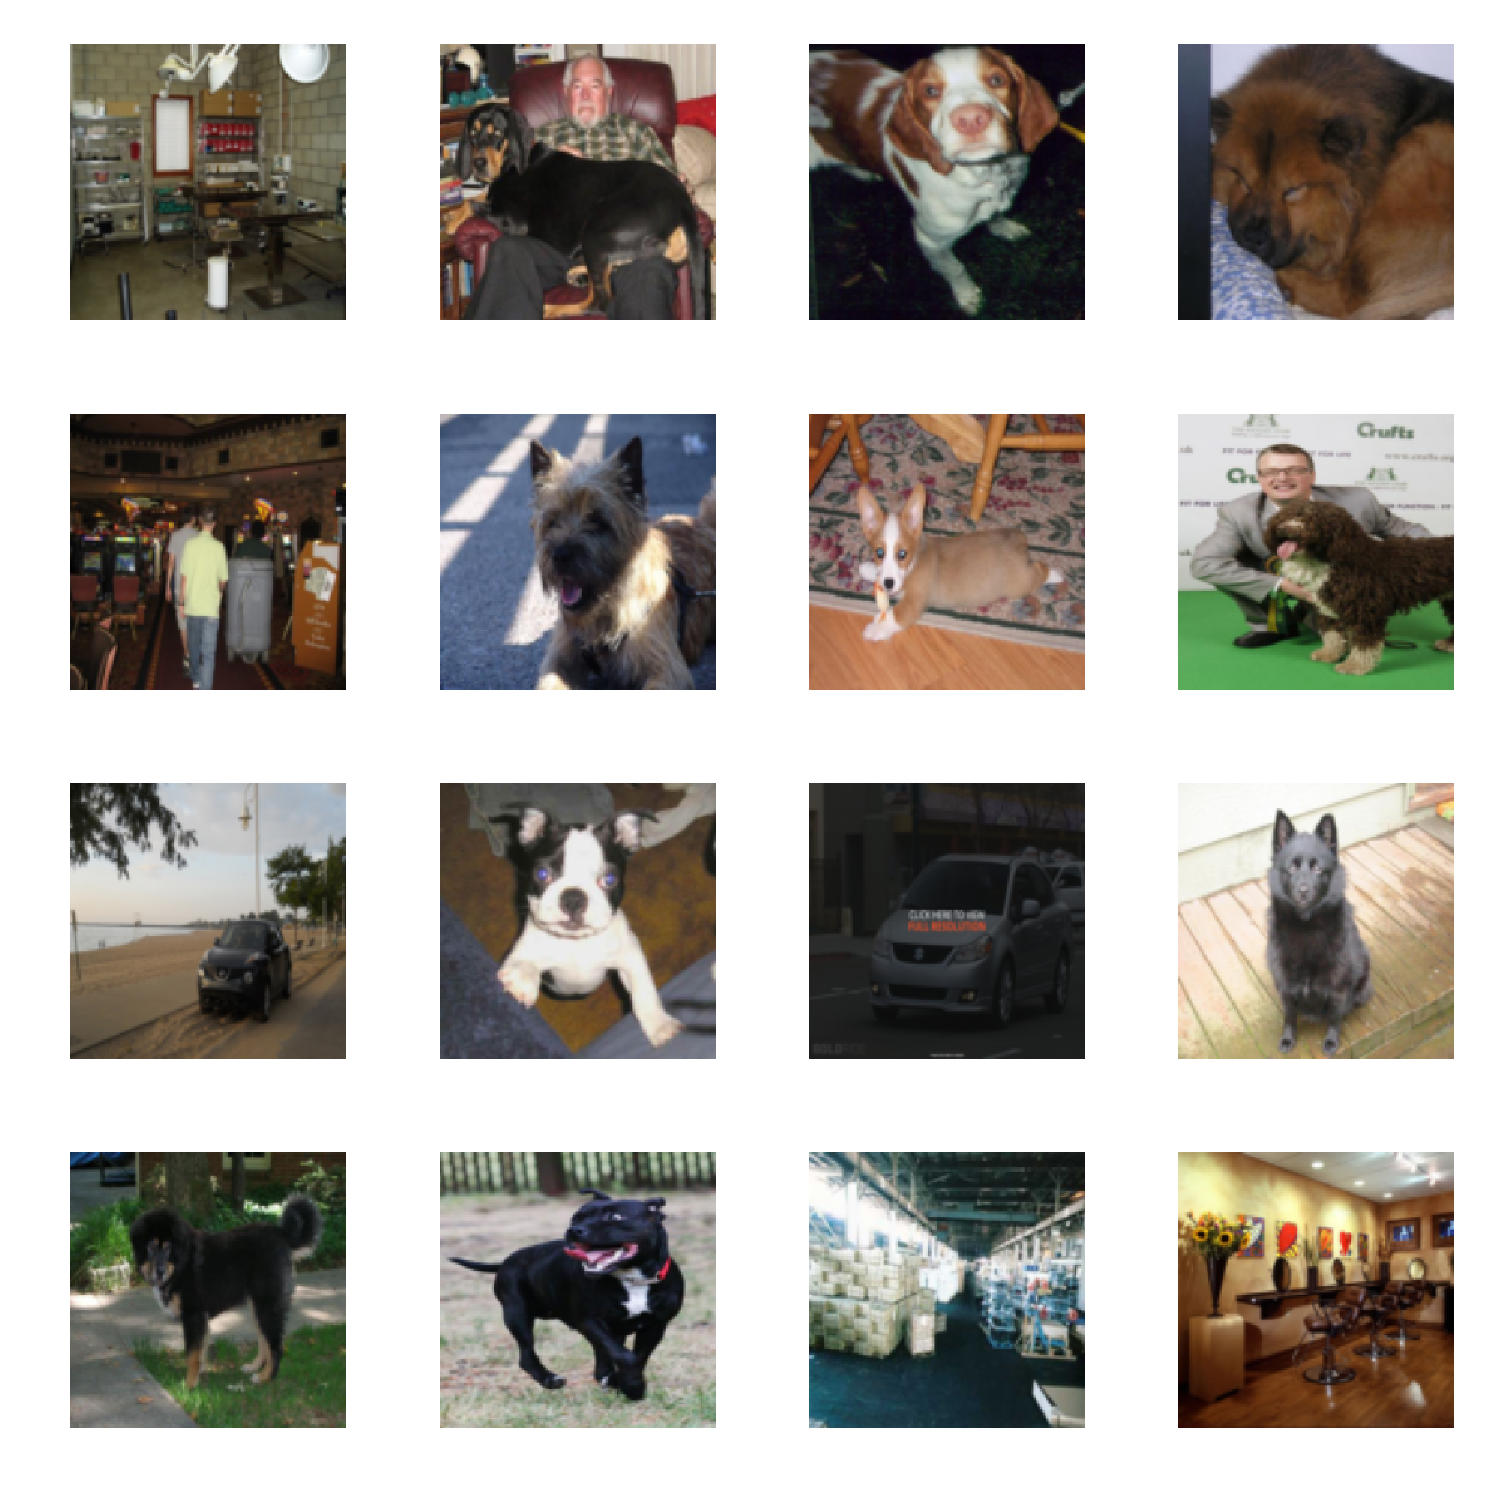
\includegraphics[width=6cm]{images/images_davae/cars_small_distance}
		\caption{Statistiques de distance faible}
	\end{subfigure}
	\begin{subfigure}{6cm}
		\centering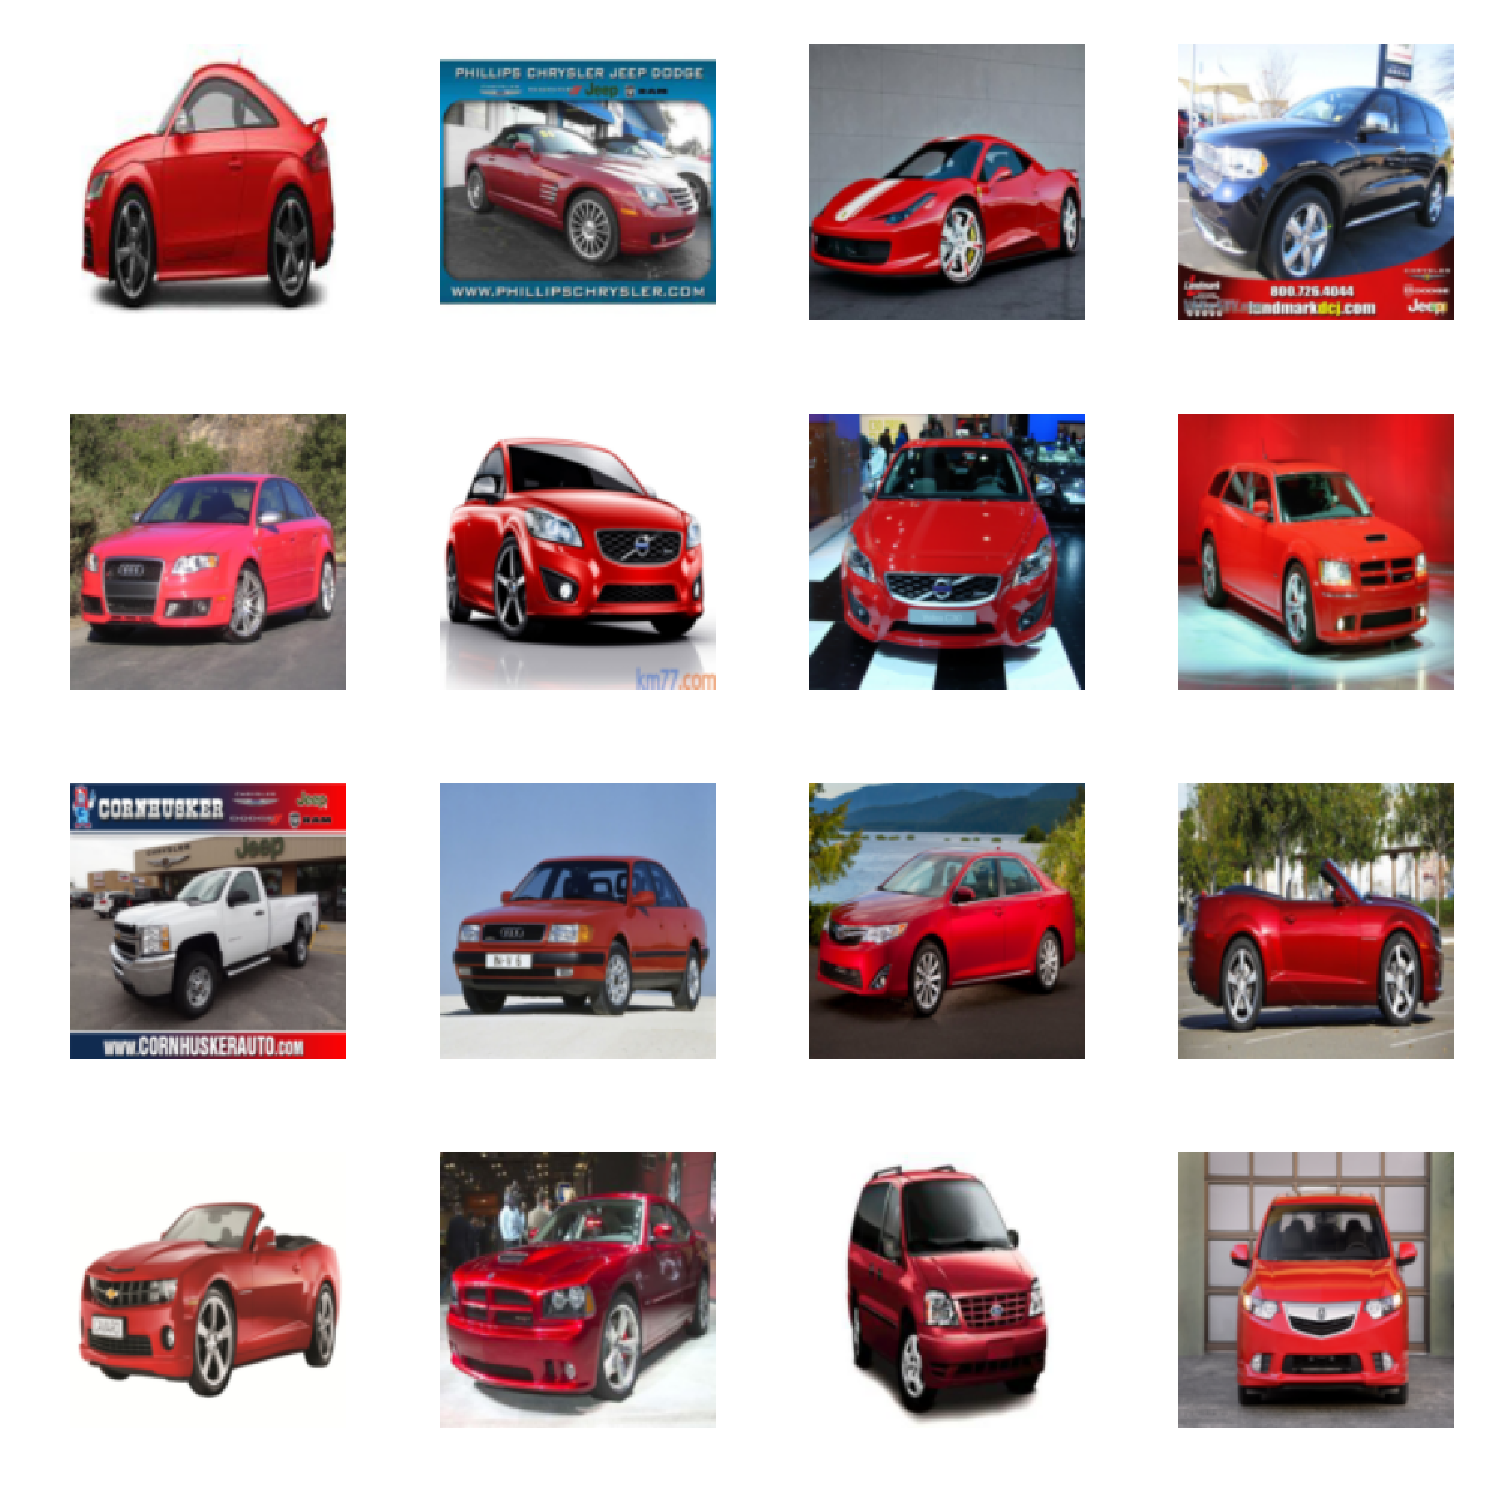
\includegraphics[width=6cm]{images/images_davae/cars_large_distance}
		\caption{Statistiques de distance élevées}
	\end{subfigure}
	\caption{Échantillons d'images provenant du jeu de données d'entraînement ayant des statistiques de distance faibles (a) et élevées (b) pour le scénario "Plus" du jeu de données \textit{ImageNet}.}
	\label{fig:latentes_images}
\end{figure}

\begin{figure}[htb]
	\centering
	\centering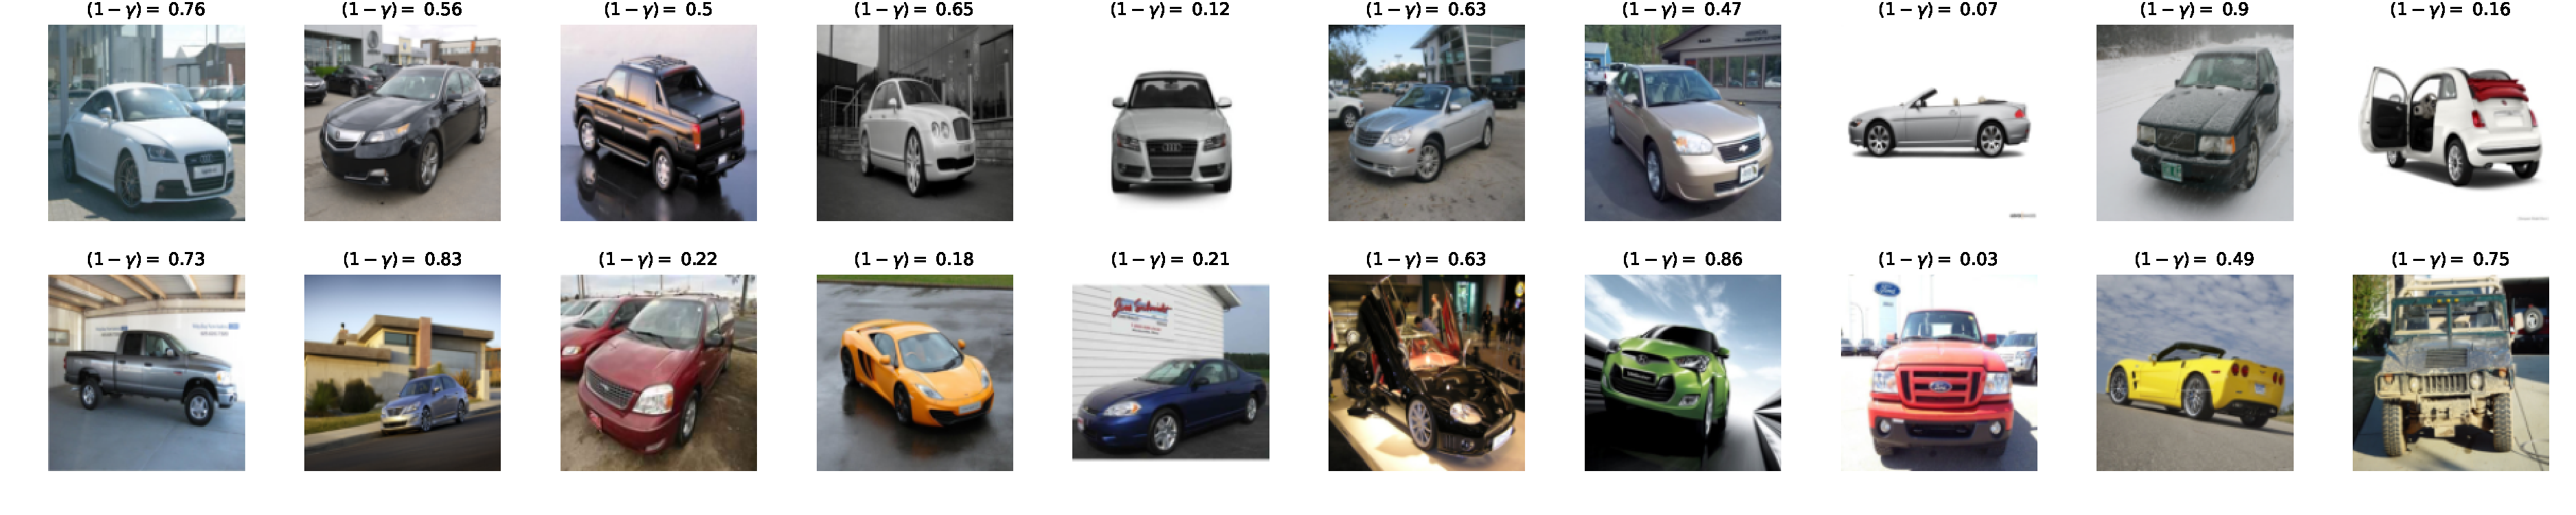
\includegraphics[width=\linewidth]{images/random_examples}
	\caption{Échantillons d'images pré-sélectionnées avec l'inverse de leur score d'anomalie ($1-\gamma$). Le score a été calculé selon le modèle DA-VAE du scénario "Plus" sur le jeu de données \textit{ImageNet}.}
	\label{fig:random_samples}
\end{figure}

De cette manière, il est possible de conclure que nous nous retrouvons dans le scénario où les représentations latentes des observations "normales" sont plus éloignées de la $N(0,I)$ (voir les deux scénarios décrits à \ref{liste_scenarios}). À la figure \ref{fig:cars_latent_stats}, on peut confirmer cette observation alors qu'on voit que les valeurs moyennes des $\boldsymbol{\mu}$ et $\boldsymbol{\sigma}$ des observations "normales" sont plus éloignées de la $N(0,I)$. Dans cette figure, on calcule pour chaque observation du jeu de données d'entraînement, la valeur moyenne sur les 25 dimensions latentes des vecteurs $\boldsymbol{\mu}$ et $\boldsymbol{\sigma}$. La différence est beaucoup plus évidente pour le vecteur latent $\boldsymbol{\sigma}$ que pour $\boldsymbol{\mu}$. Pour $\boldsymbol{\mu}$, les observations "normales" sont légèrement plus centrées à 0, mais les observations "anormales" s'éloignent moins de la valeur centrée de 0. À la figure \ref{fig:pca_cars}, nous avons réalisé une analyse en composantes principales sur les vecteurs $\boldsymbol{\mu}$ et $\boldsymbol{\sigma}$ et avons conservé les \DIFdelbegin \DIFdel{2 }\DIFdelend \DIFaddbegin \DIFadd{deux }\DIFaddend premières composantes principales. Cela nous permet d'obtenir une visualisation en \DIFdelbegin \DIFdel{2 }\DIFdelend \DIFaddbegin \DIFadd{deux }\DIFaddend dimensions des représentations latentes des observations "normales" et "anormales". On peut voir que les \DIFdelbegin \DIFdel{2 }\DIFdelend \DIFaddbegin \DIFadd{deux }\DIFaddend groupes sont relativement bien séparés sur les \DIFdelbegin \DIFdel{2 }\DIFdelend \DIFaddbegin \DIFadd{deux }\DIFaddend premières composantes principales. On peut également voir la projection en \DIFdelbegin \DIFdel{2 }\DIFdelend \DIFaddbegin \DIFadd{deux }\DIFaddend dimensions du point $(\boldsymbol{0_{m}}, \boldsymbol{1_{m}})$, soit le carré noir. On remarque que les anomalies (points bleus) semblent légèrement plus près du carré noir que les observations "normales". Il faut rappeler que la projection en \DIFdelbegin \DIFdel{2 }\DIFdelend \DIFaddbegin \DIFadd{deux }\DIFaddend dimensions conserve approximativement 50\% de la variabilité totale des représentations latentes.

\begin{figure}[H]
	\centering
	\begin{subfigure}{12cm}
		\centering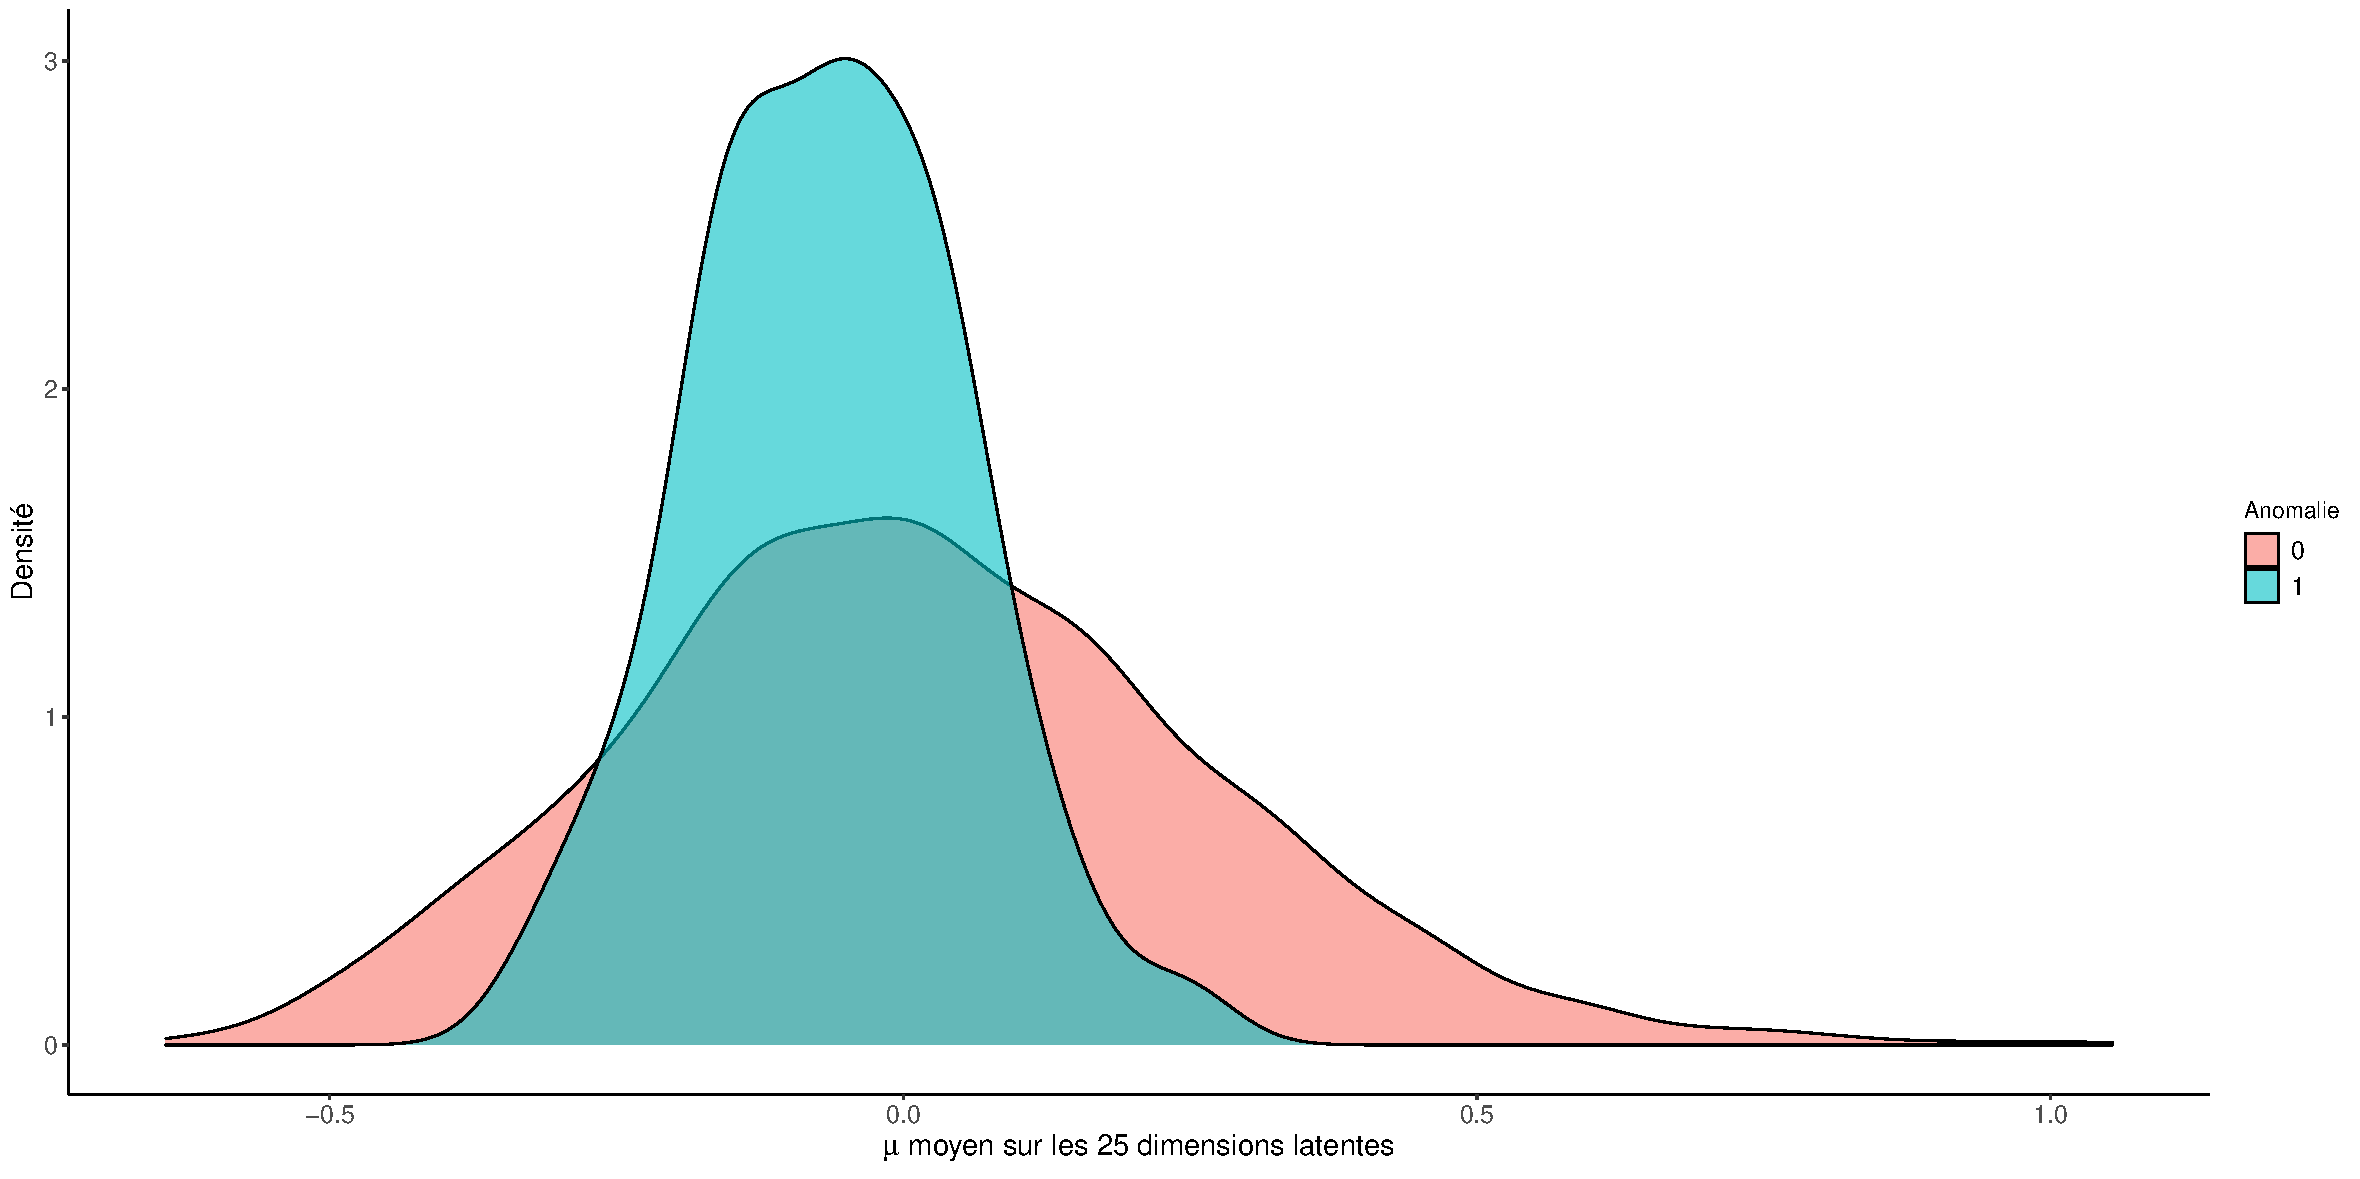
\includegraphics[width=12cm, height=6cm]{images/latent_stats/plot_mu}
		\caption{Distribution des $\boldsymbol{\mu}$ moyens}
	\end{subfigure}
	\begin{subfigure}{12cm}
		\centering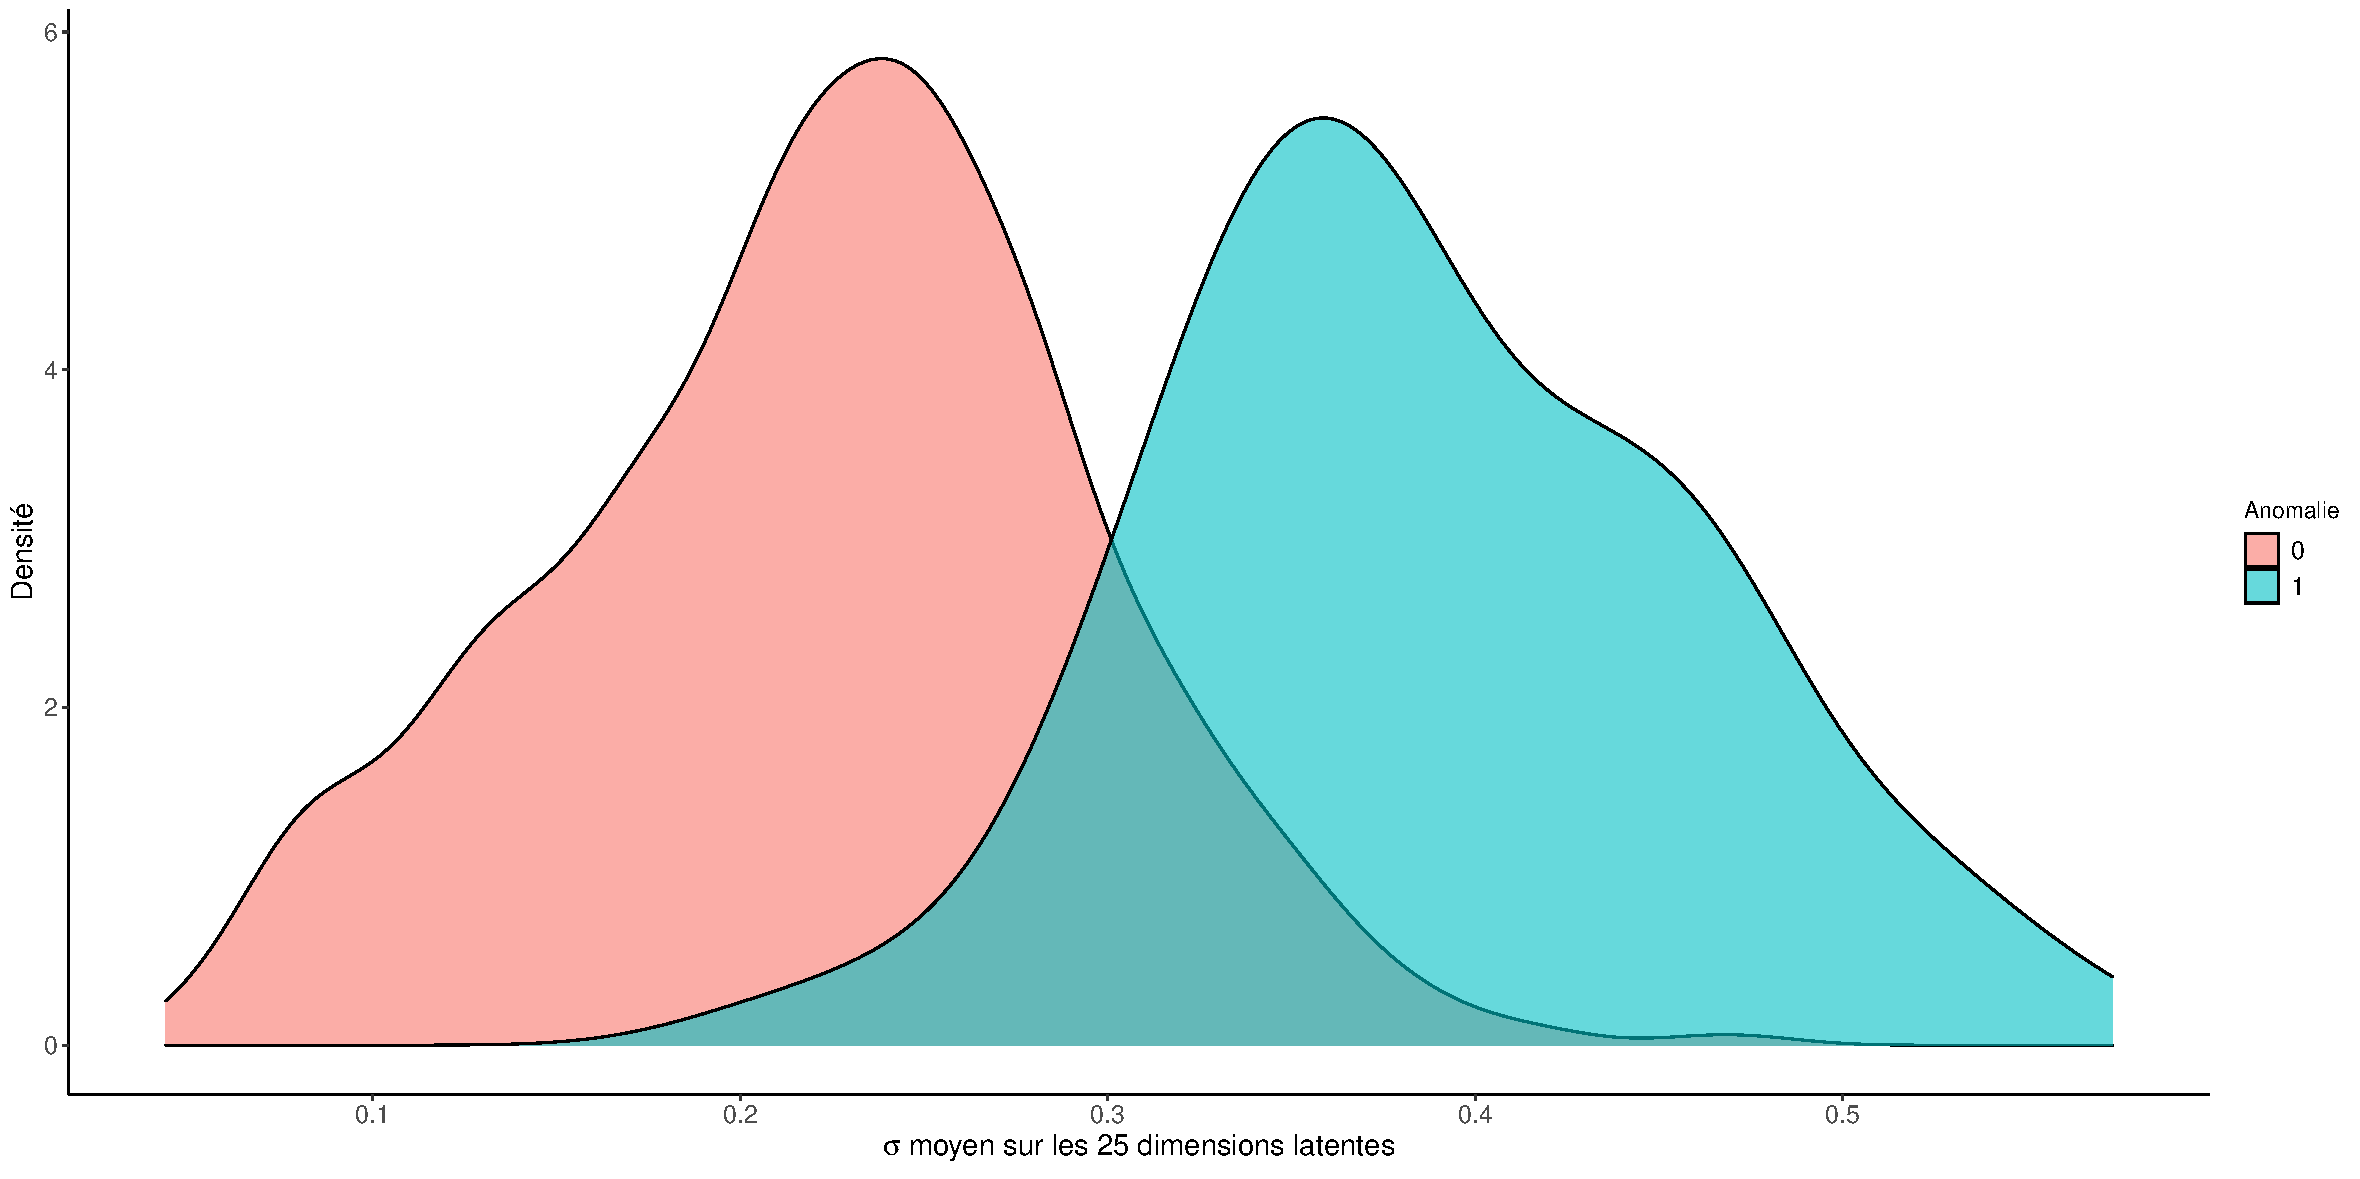
\includegraphics[width=12cm, height=6cm]{images/latent_stats/plot_sigma}
		\caption{Distribution des $\boldsymbol{\sigma}$ moyens}
	\end{subfigure}
	\caption{Moyenne des $\boldsymbol{\mu}$ et $\boldsymbol{\sigma}$ des représentations latentes du jeu de données d'entraînement sur le jeu de données \textit{ImageNet}.}
	\label{fig:cars_latent_stats}
\end{figure}

\begin{figure}[htb]
	\centering
	\centering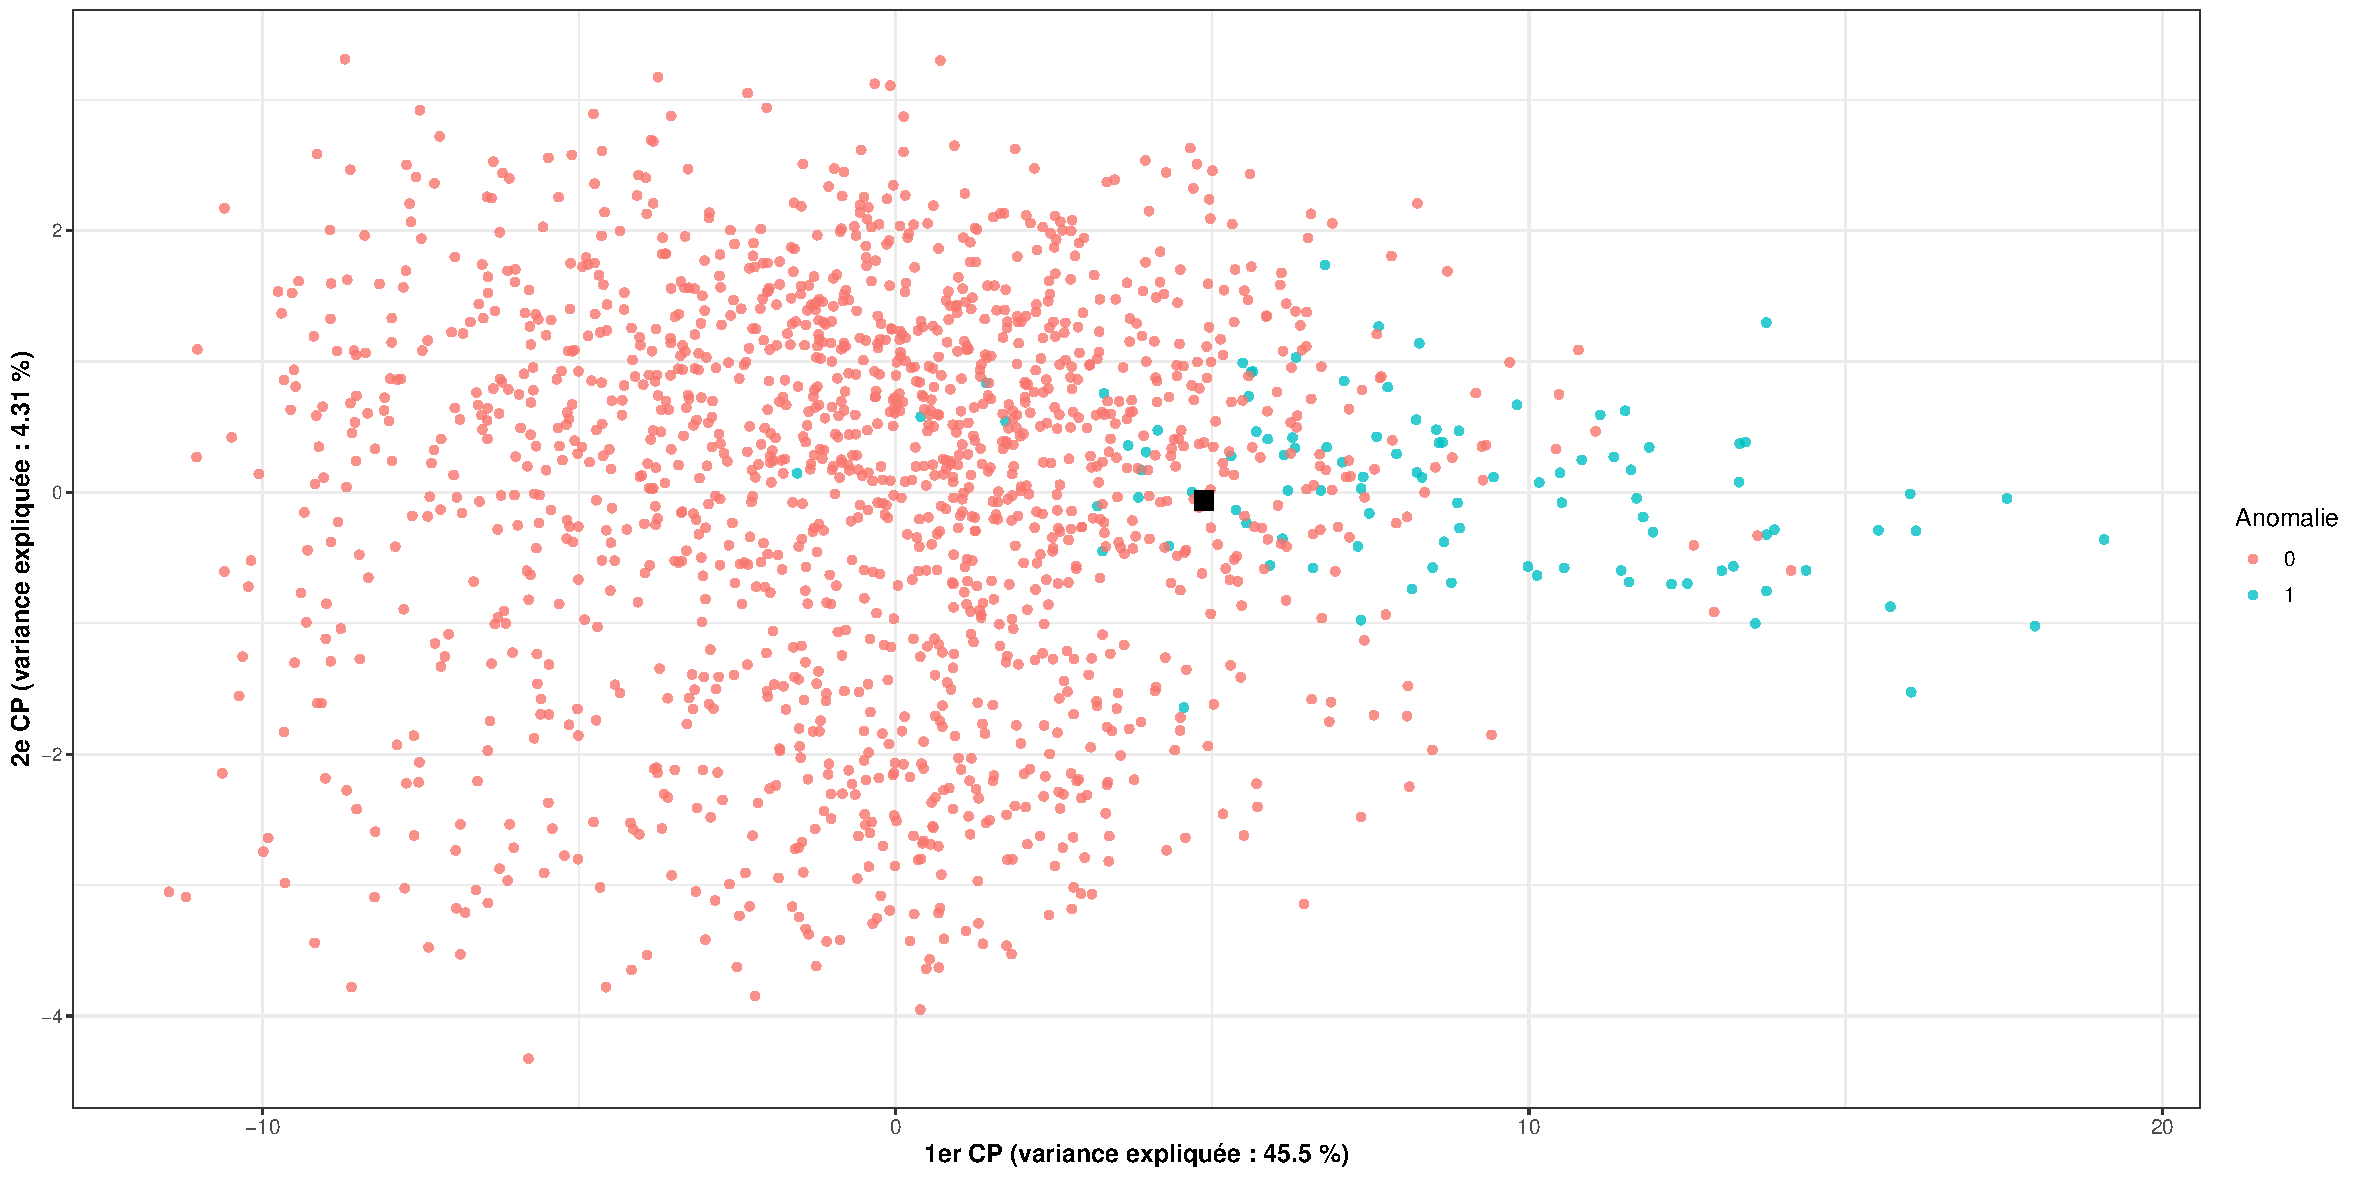
\includegraphics[width=\linewidth]{images/plot_pca_cars}
	\caption{Graphique des \DIFdelbeginFL \DIFdelFL{2 }\DIFdelendFL \DIFaddbeginFL \DIFaddFL{deux }\DIFaddendFL premières composantes principales calculées à partir des vecteurs $\boldsymbol{\mu}$ et $\boldsymbol{\sigma}$ du jeu de données d'entraînement de \textit{ImageNet} appliqué sur le scénario de contamination "Plus".}
	\label{fig:pca_cars}
\end{figure}


\subsubsection{Analyse de la perte en entraînement}

Dans la section \ref{beta_schedule}, nous avons présenté l'horaire de l'hyperparamètre $\beta$ utilisé selon l'itération d'entraînement de l'autoencodeur variationnel. Cet hyperparamètre, utilisé dans les méthodes ISOF-VAE et DA-VAE, donne plus ou moins d'importance à la composante de perte associée au critère de Kullback-Leibler. Cette sous-section a simplement comme objectif de faire un compte-rendu de la composition de la perte en entraînement afin de faciliter la reproductibilité de notre approche. En guise de rappel, notre objectif avec l'horaire de l'hyperparamètre $\beta$ était de mettre l'accent sur la composante de reconstruction $(\beta = 0)$ dans les premières itérations pour ensuite augmenter la régularisation en augmentant l'hyperparamètre $\beta$ pendant quelques itérations. La figure \ref{fig:cars_kld_perc} montre la composition de notre perte totale au fil des itérations d'entraînement. La figure illustre le pourcentage de la perte provenant du critère de Kullback-Leibler. L'autre composante de la perte est associée à la reconstruction. On peut voir que les 5 premières itérations sont composées uniquement de la composante de reconstruction. Cela est dû à notre hyperperamètre $\beta=0$. Par la suite, la composante de Kullback-Leibler prend plus d'importance et tend finalement vers une valeur près de 0 dans les dernières itérations. Il est rassurant de voir que l'horaire que nous avons établi pour l'hyperparamètre $\beta$ est cohérent avec la composition de la perte obtenue.

\begin{figure}[H]
	\centering
	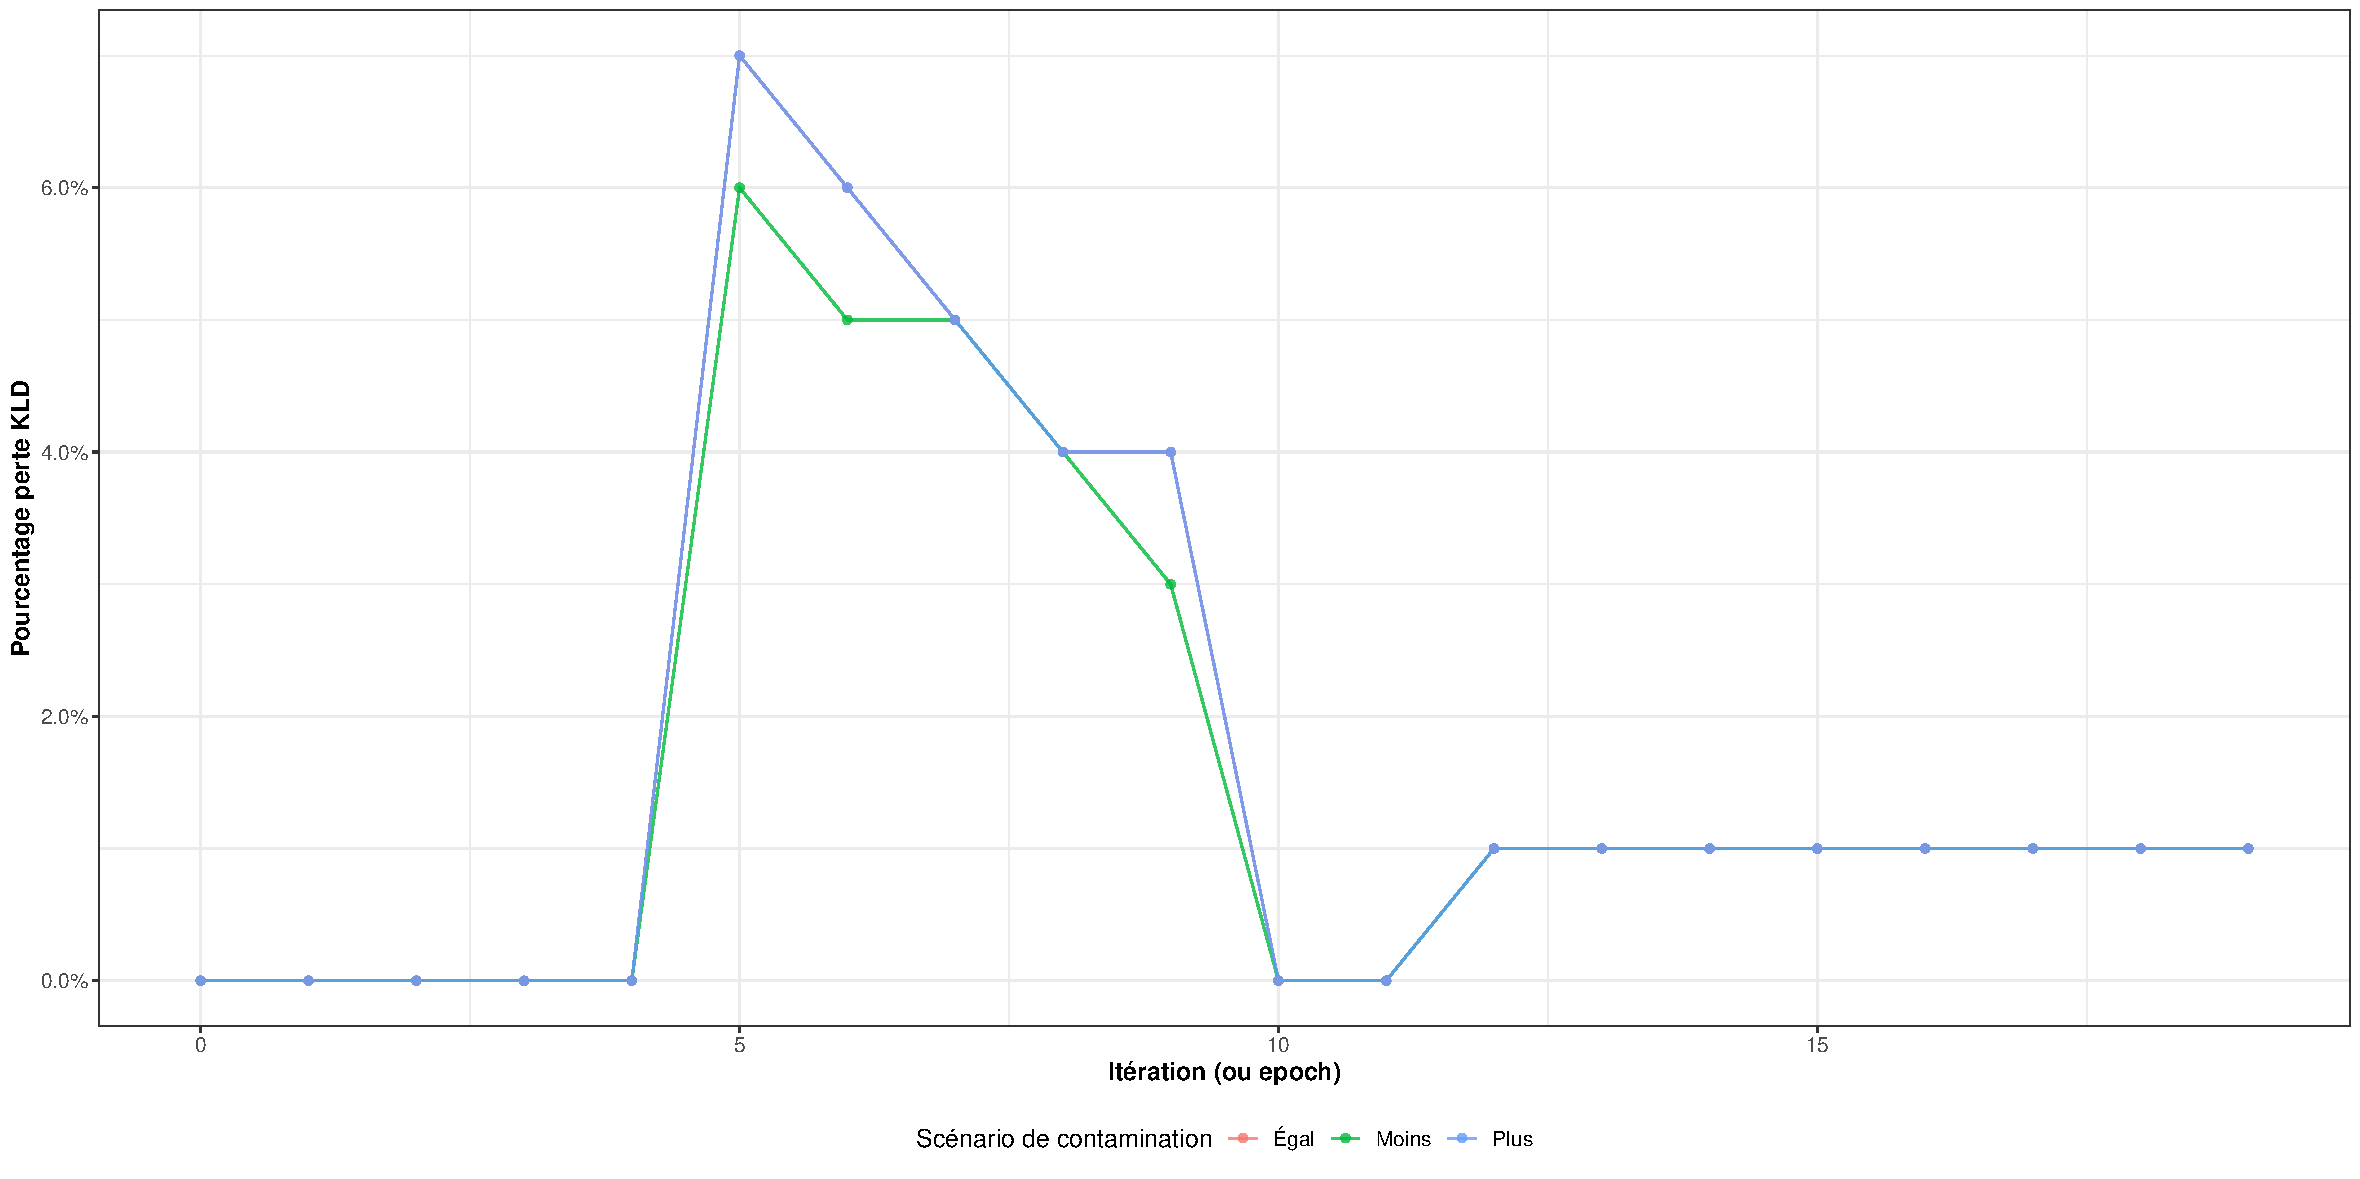
\includegraphics[width=\linewidth]{images/kld_cars.pdf}
	\caption{Pourcentage du critère de Kullback-Leibler dans la perte totale selon l'itération d'entraînement et le scénario de contamination. Ces résultats sont tirés du scénario de contamination "Plus" pour le jeu de données \textit{ImageNet}.}
	\label{fig:cars_kld_perc}
\end{figure}


\subsubsection{Génération d'images}

Comme mentionné dans la section \ref{background-vae}, les autoencodeurs variationnels ont la particularité d'avoir une représentation latente continue. En effet, cela est dû au fait que le vecteur latent $\boldsymbol{z}$ est obtenu en combinant une simulation d'une loi $N(0,I)$ avec les vecteurs $\boldsymbol{\mu}$ et $\boldsymbol{\sigma}$ appris par le modèle (voir équation \ref{eq:latent_formula}). Étant donné la composante de perte de Kullback-Leibler appliquée dans l'optimisation des paramètres, ces \DIFdelbegin \DIFdel{2 }\DIFdelend \DIFaddbegin \DIFadd{deux }\DIFaddend vecteurs devraient s'approcher des vecteurs $(\boldsymbol{0_{m}}, \boldsymbol{1_{m}})$ où $m$ correspond à la longueur de la représentation latente. Après l'entraînement de l'autoencodeur, il est possible de valider le comportement du décodeur par rapport à une simulation $N(0,I)$. La figure \ref{fig:generated_cars} montre des exemples d'images générées à partir de simulations de loi $N(0,I)$ et reconstruites par la partie décodeur du DA-VAE. Pour ce faire, nous avons simulé des observations de loi $N(0,I)$ à \DIFdelbegin \DIFdel{25 }\DIFdelend \DIFaddbegin \DIFadd{$m=25$ }\DIFaddend dimensions, soit la dimension latente de notre autoencodeur variationnel entraîné. Par la suite, nous avons donné ces simulations en argument à notre fonction de décodeur $p_{\phi}(\cdot)$ où les paramètres de cette fonction représentés par $\phi$ \DIFdelbegin \DIFdel{, }\DIFdelend sont déjà ajustés. Cela nous permet d'obtenir de nouvelles images générées de toute pièce. Ces images illustrent bien qu'une représentation latente provenant d'une loi $N(0,I)$ donne un résultat qui s'apparente à une voiture ou aux caractéristiques fréquentes d'une voiture (roues, phares, pare-brise).

\begin{figure}[htb]
	\centering
	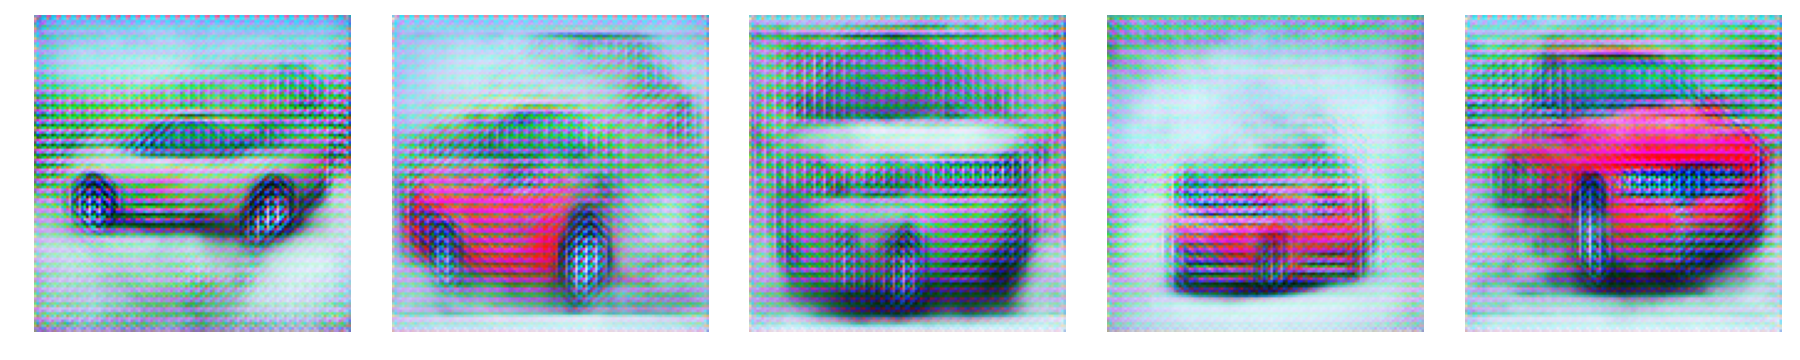
\includegraphics[width=\textwidth]{images/generated_cars}
	\caption{Exemples d'images générées par le modèle DA-VAE en utilisant seulement la partie décodeur de l'autoencodeur ainsi que des simulations provenant d'une loi $N(0,I)$.}
	\label{fig:generated_cars}
\end{figure}

\subsection{Résultats sur \textit{MNIST}}

Dans le tableau \ref{tab:auc_mnist}, on peut voir les performances en aire sous la courbe ROC pour les différents scénarios de test réalisés sur \textit{MNIST}. Premièrement, on remarque que toutes les approches donnent des résultats performants avec des aires sous la courbe généralement supérieures à 0.85, et même parfois très près de 1. Cette observation vient témoigner du fait qu'étant donné la nature plus simple des données, il est probablement plus facile de faire la détection d'anomalies. En regardant de plus près les résultats des \DIFdelbegin \DIFdel{4 }\DIFdelend \DIFaddbegin \DIFadd{quatre }\DIFaddend approches, on remarque que notre approche DA-VAE est rarement meilleure que les méthode AE ou ACP en aire sous la courbe ROC moyenne. La variabilité autour de la métrique est aussi légèrement plus élevée pour l'approche DA-VAE. Par contre, les résultats sont généralement près des meilleures approches. De plus, \DIFdelbegin \DIFdel{l'intervalle avec 2 écart-types autour de la moyenne }\DIFdelend \DIFaddbegin \DIFadd{le test de Mann-Whitney }\DIFaddend nous permet de conclure que les autres méthodes ne sont pas significativement meilleures que DA-VAE. Notre approche montre également les meilleurs résultats en aire sous la courbe ROC pour le scénario de test 6, et ce, pour les \DIFdelbegin \DIFdel{3 }\DIFdelend \DIFaddbegin \DIFadd{trois }\DIFaddend scénarios de contamination différents. Le scénario de test 6 est celui qui considère le chiffre "6" comme "normal" et tous les autres comme la classe "anormale". Étant donné la nature plus simple des images, les méthodes basées sur la reconstruction (ACP et AE) semblent être celles qui fonctionnement généralement le mieux. On pourrait donc croire que l'utilisation de la représentation latente dans les méthodes ISOF-VAE et DA-VAE n'amène pas autant de valeur ajoutée que dans le cas d'images réelles comme \textit{ImageNet}. En faisant l'analyse des métriques de précision et de rappel (tableaux \ref{tab:precision_mnist} et \ref{tab:recall_mnist}), on peut tirer essentiellement les mêmes conclusions quant aux performances relatives des différentes approches. Nous ferons l'analyse plus détaillée de ces méthodes dans la sous-section \ref {mnist:reconsruction}. Encore une fois, les méthodes basées sur la reconstruction semblent légèrement supérieures. Toutefois, l'approche DA-VAE n'est pas significativement inférieure aux autres, même en précision et rappel\DIFdelbegin \DIFdel{, si on prend en considération les erreurs standards des moyennes}\DIFdelend .

Pour illustrer les résultats du modèle selon différents scénarios de contamination, il est possible de réutiliser les mêmes figures que celles décrites à la figure \ref{fig:pvalues_scenarios}. Dans la figure \ref{fig:pvalues_scenarios_mnist}, on peut y voir ces figures générées pour le scénario de test 3 (voir tableau \ref{tab:mnist_scenarios} pour un rappel des scénarios de test).

\begin{figure}[H]
	\centering
	\begin{subfigure}{6cm}
		\centering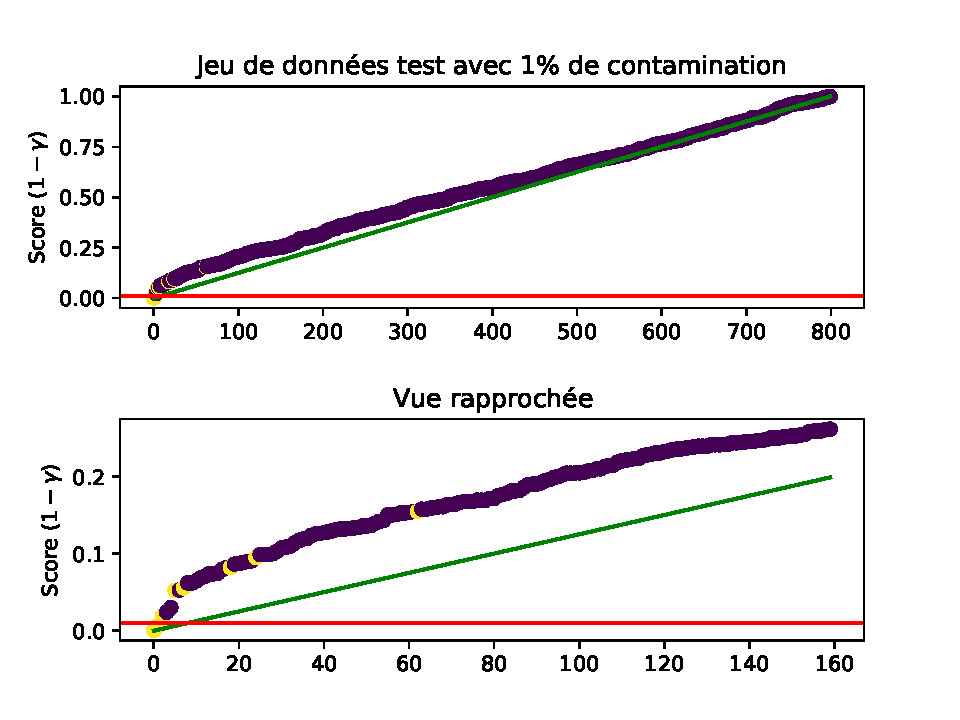
\includegraphics[width=6cm]{images/images_davae/pvalues_scenario3_moins}
		\caption{Scénario "Moins"}
	\end{subfigure}
	\begin{subfigure}{6cm}
		\centering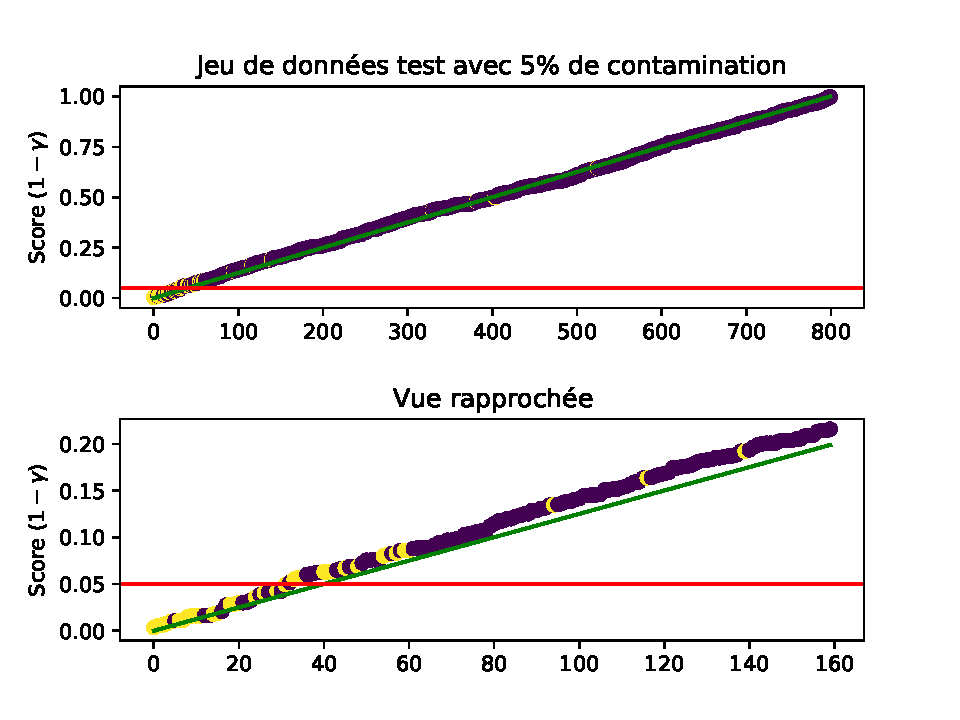
\includegraphics[width=6cm]{images/images_davae/pvalues_scenario3_egal}
		\caption{Scénario "Égal"}
	\end{subfigure}
	\begin{subfigure}{6cm}
		\centering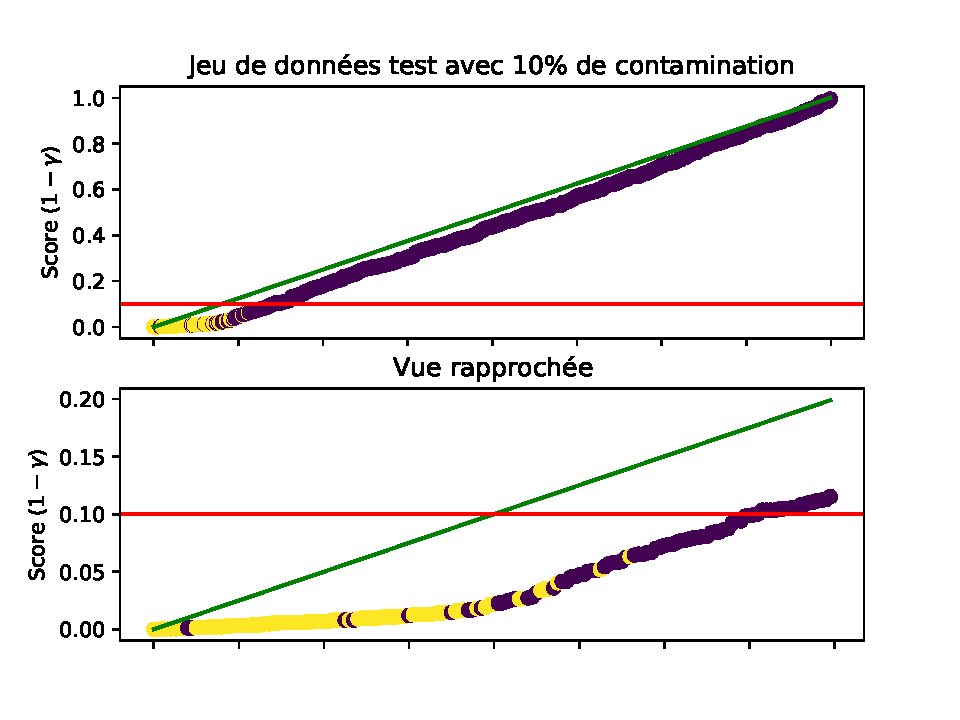
\includegraphics[width=6cm]{images/images_davae/pvalues_scenario3_plus}
		\caption{Scénario "Plus"}
	\end{subfigure}
	\caption{Graphiques illustrant les scores d'anomalies selon le scénario de contamination pour le modèle DA-VAE appliqué sur le scénario de test 1 de MNIST. Les points violets sont des observations que nous connaissons comme "normales" alors que les points jaunes sont des observations que nous connaissons comme "anormales". Dans tous les cas, le niveau de filtration $\alpha$ est défini comme le niveau de contamination dans le jeu de données de test. Pour chaque sous-figure, nous présentons une vue complète des observations du jeu de données de test ainsi qu'une vue rapprochée sur les observations situées plus à gauche de l'axe des $x$.}
	\label{fig:pvalues_scenarios_mnist}
\end{figure}

Dans les \DIFdelbegin \DIFdel{3 }\DIFdelend \DIFaddbegin \DIFadd{trois }\DIFaddend sous-figures à la figure \ref{fig:pvalues_scenarios_mnist}, on peut voir que les observations "anormales", soit les points jaunes, sont principalement regroupées à gauche de l'axe des $x$, ce qui est le comportement souhaité. On remarque aussi que la segmentation est plus évidente que dans le cas de la figure \ref{fig:pvalues_scenarios}, ce qui nous permet de confirmer que la détection d'anomalies est plus performante sur ce scénario de test du jeu de données MNIST que sur le jeu de données \textit{ImageNet}. Finalement, on peut également remarquer la disposition des observations par rapport à la courbe verte. On peut tirer les mêmes constats que dans la section \ref{imagenet_results}, mais en ajoutant le fait que les positions des premières observations par rapport à la courbe verte sont encore plus prononcées dans le cas du jeu de données MNIST. 
\DIFdelbegin \DIFdel{Ces graphiques }\DIFdelend \DIFaddbegin 

\DIFadd{Les graphiques de la figure \ref{fig:pvalues_scenarios_mnist} }\DIFaddend sont intéressants puisqu'ils pourraient servir d'outil pour estimer la proportion d'anomalies dans le jeu de données test par rapport à la proportion présente dans le jeu de données d'entraînement. Dans la réalité, nous ne pourrions pas savoir quels observations sont des anomalies et lesquelles sont "normales". Par contre, avec la disposition de la courbe, nous pourrions savoir si le jeu de données de test contient, en proportion, moins, autant ou plus d'anomalies que le jeu de données d'entraînement. \DIFaddbegin \DIFadd{Dans le cas où le jeu de données de test contiendrait une proportion  d'anomalies plus faible que le jeu de données d'entraînement, le début de la courbe devrait s'approcher de l'axe des $y$. Dans le cas où le jeu de données de test contiendrait une proportion d'anomalies similaire au jeu de données d'entraînement, la courbe serait alignée avec la droite $(0,0)$ et $(1,1)$. Finalement, dans le cas où le jeu de données de test contiendrait une proportion d'anomalies plus élevée que le jeu de données d'entraînement, le début de la courbe devrait s'approcher de l'axe des $x$.
}\DIFaddend 

En portant attention au niveau de filtration $\alpha$ dans les \DIFdelbegin \DIFdel{3 }\DIFdelend \DIFaddbegin \DIFadd{trois }\DIFaddend différentes sous-figures de la figure \ref{fig:pvalues_scenarios_mnist}, on remarque que celui-ci semble être efficace dans le scénario de contamination "Égal". Dans les \DIFdelbegin \DIFdel{2 }\DIFdelend \DIFaddbegin \DIFadd{deux }\DIFaddend autres scénarios, ce seuil ne semble pas être le niveau optimal. Toutefois, l'avantage avec cette approche de filtration est qu'il est facile de le modifier et on sait que celui-ci doit être défini dans l'intervalle $[0, 1]$.

\subsubsection{Analyses des méthodes basées sur la reconstruction} \label{mnist:reconsruction}

Dans la sous-section \ref{imagenet:reconsruction}, nous avions fait la conclusion que les méthodes basées sur la reconstruction ne permettaient pas d'obtenir de bonnes performances sur des images réelles. Dans le cas du jeu de données \textit{MNIST}, les performances de ces méthodes sont généralement supérieures à celles basées sur la représentation latente. Pour se convaincre de ces résultats, la figure \ref{fig:mnist_acp_reconstructionsa} montre des exemples d'images du jeu de données d'entraînement ayant de petites erreurs de reconstruction. Ces exemples proviennent de la méthode ACP et du scénario de test 6.  Dans le même ordre d'idées, la figure \ref{fig:mnist_acp_reconstructionsb} montre des images provenant de la même approche, mais ayant plutôt des erreurs de reconstruction élevées. 

\begin{figure}[H]
	\centering
	\begin{subfigure}{12cm}
		\centering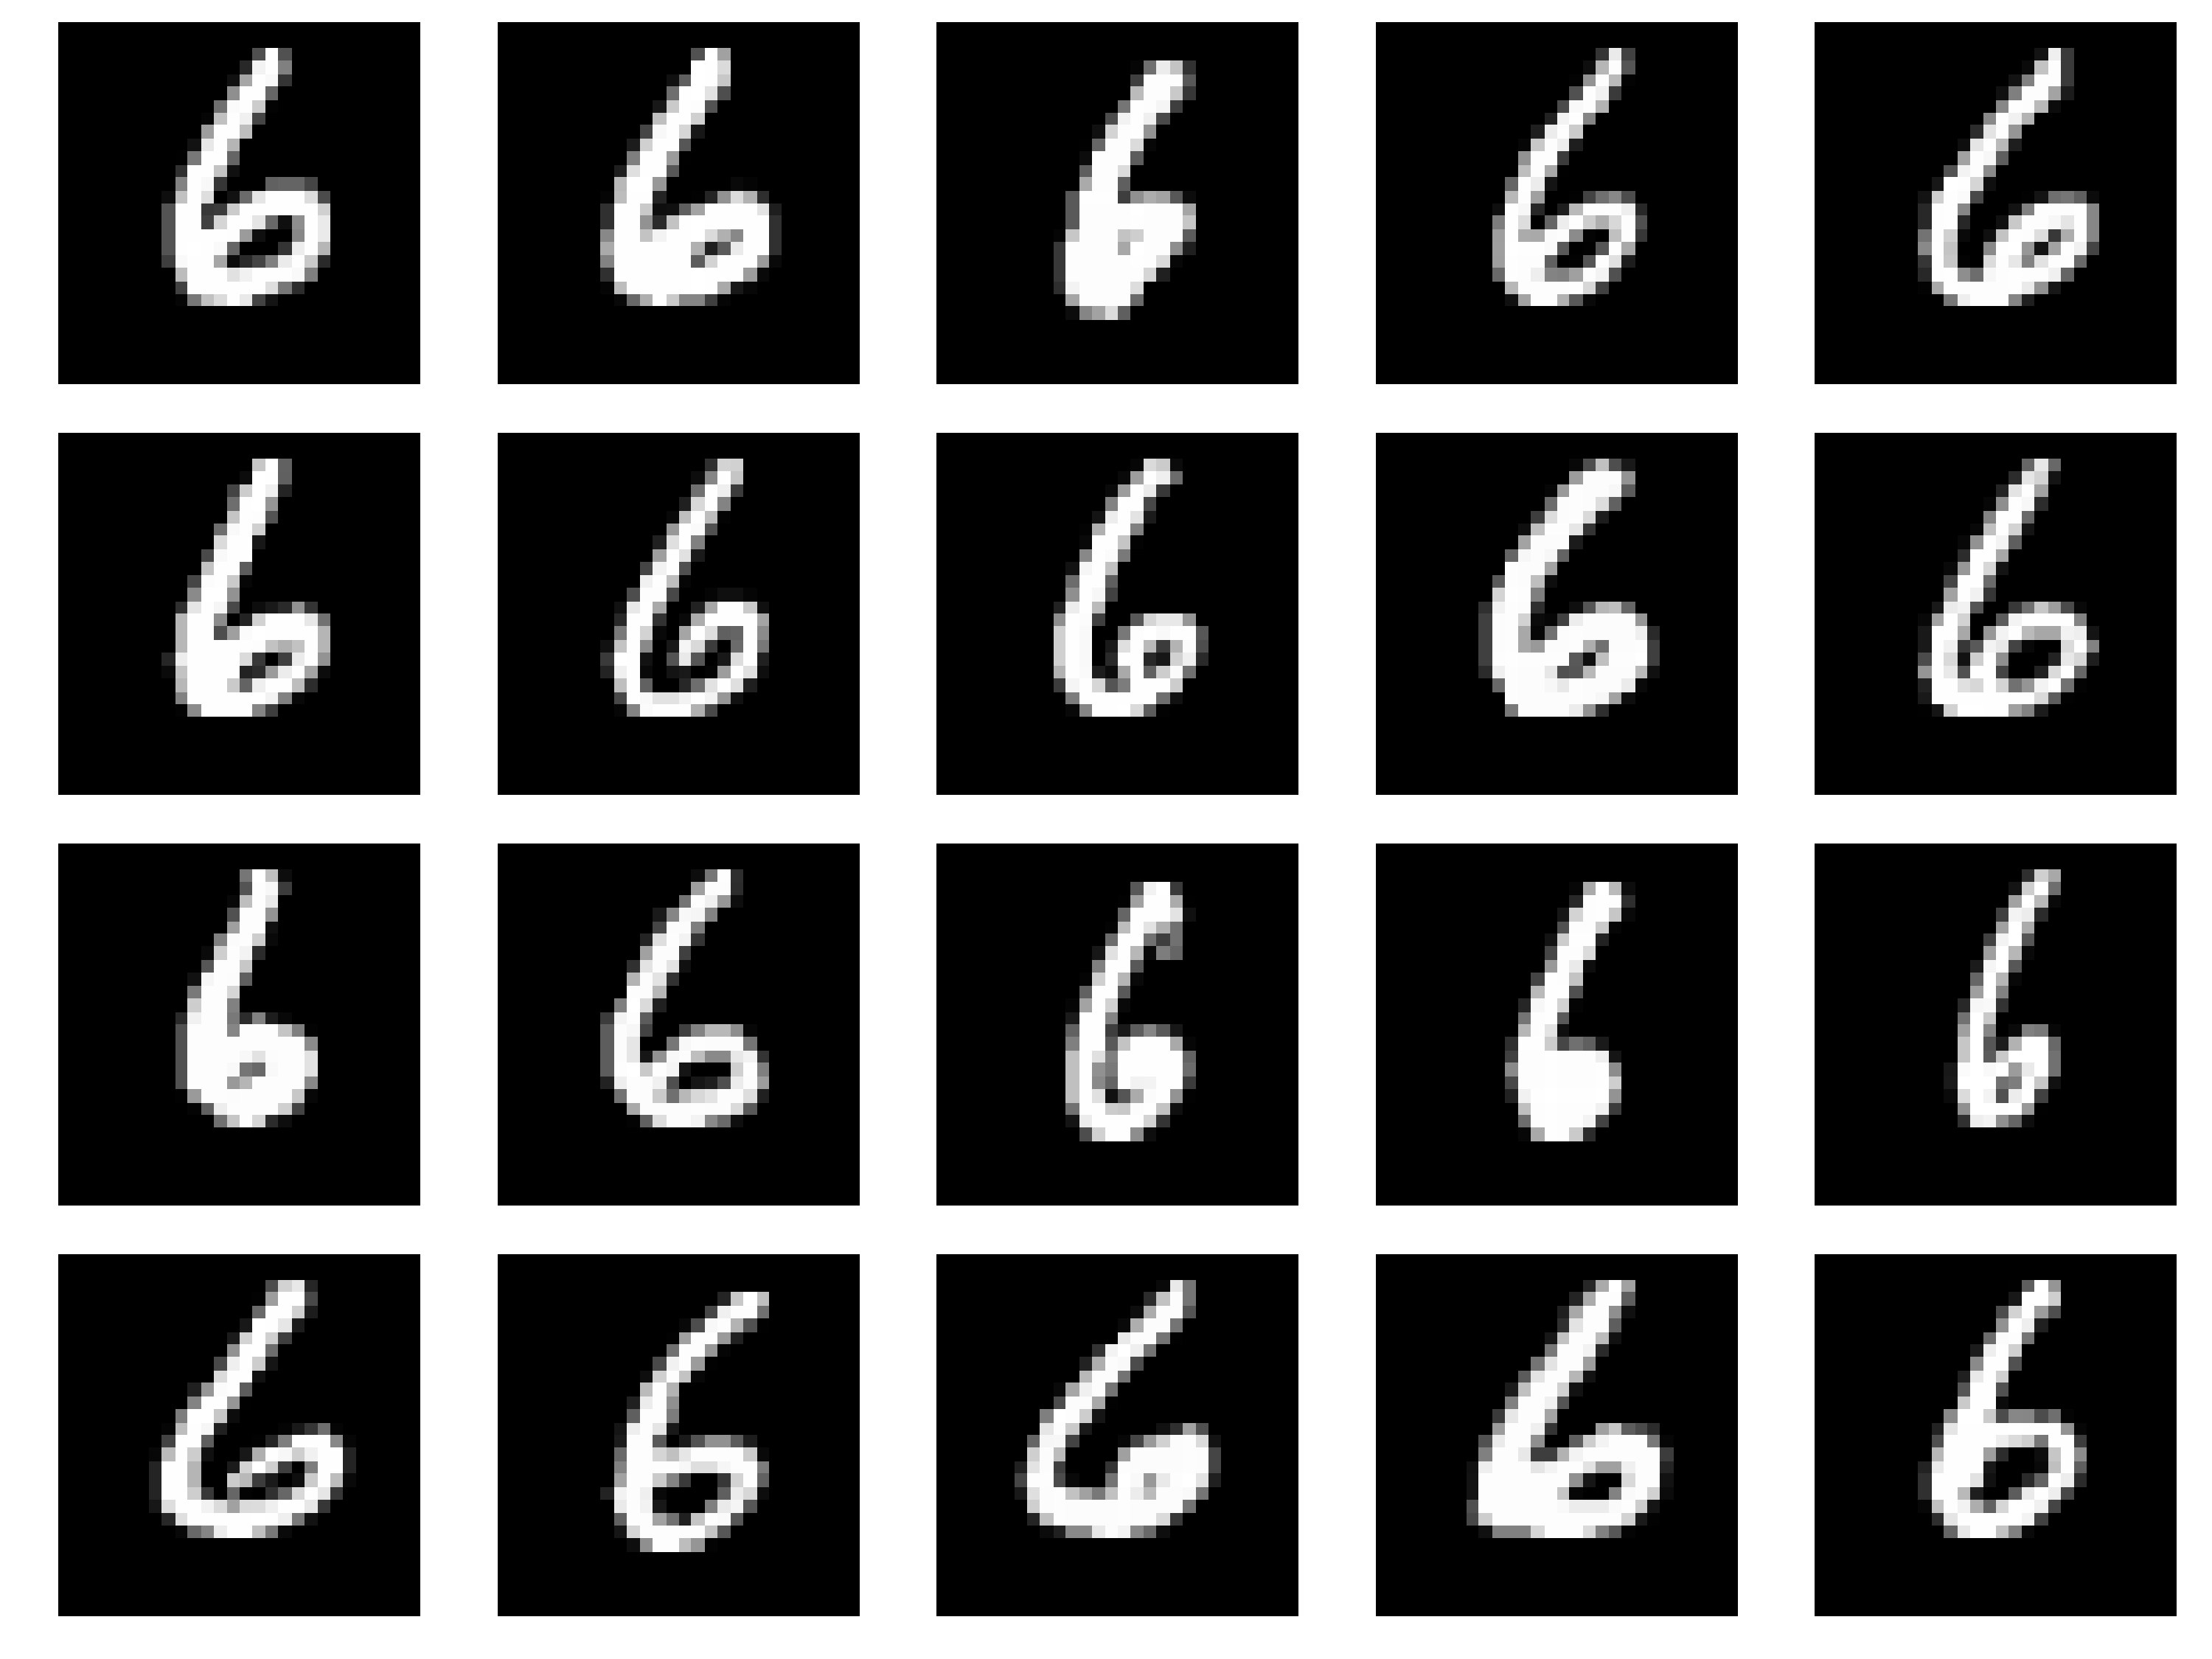
\includegraphics[width=12cm]{images/smallest_errors_mnist}
		\caption{Exemples d'images bien reconstruites}
		\label{fig:mnist_acp_reconstructionsa}
	\end{subfigure}
	\begin{subfigure}{12cm}
		\centering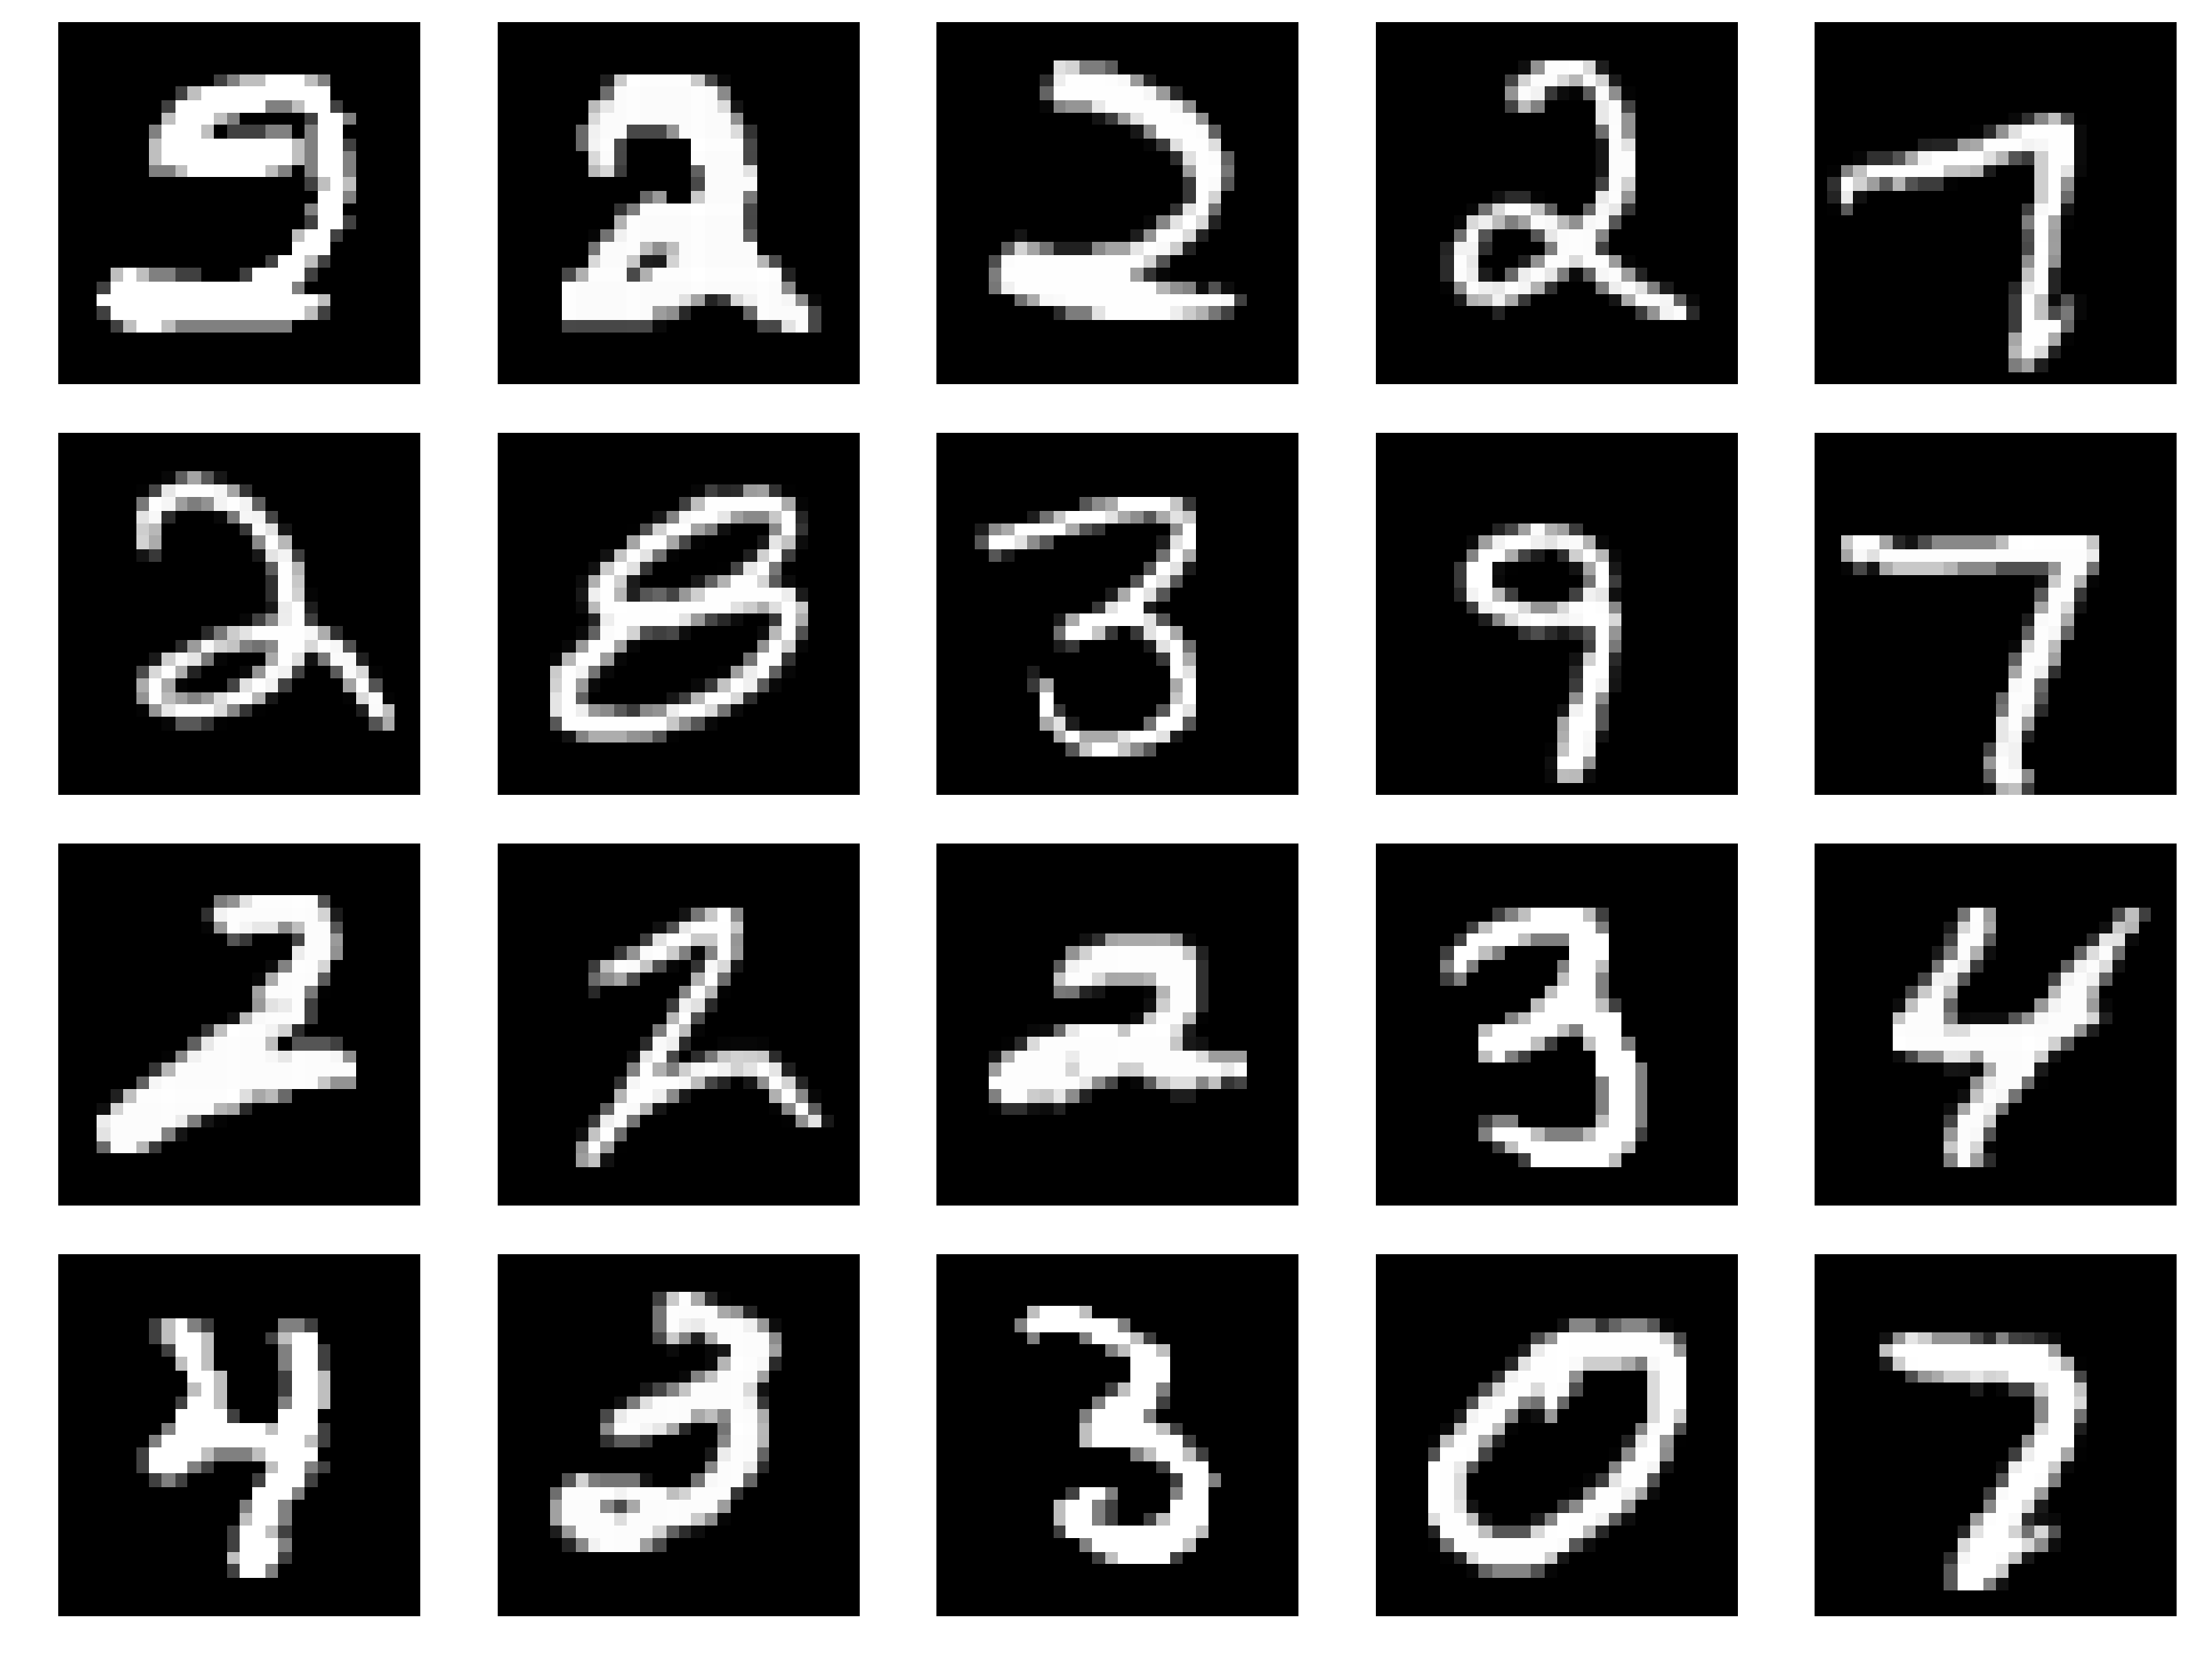
\includegraphics[width=12cm]{images/biggest_errors_mnist}
		\caption{Exemples d'images mal reconstruites}
		\label{fig:mnist_acp_reconstructionsb}
	\end{subfigure}
	\caption{Exemples d'images qui sont bien reconstruites (a) et mal reconstruites (b) selon la méthode ACP appliquée sur le jeu de données d'entraînement de \textit{MNIST}.}
	\label{fig:mnist_acp_reconstructions}
\end{figure}

En analysant la figure \ref{fig:mnist_acp_reconstructions}, on confirme en quelque sorte les bons résultats obtenus par la méthode ACP. On voit que la prémisse de base, qui dit que les images de la "normale" seront bien reconstruites, est validée. En comparaison avec le jeu de données  \textit{ImageNet}, on remarque que la classe "anormale" est beaucoup plus similaire à la classe "normale" dans le cas de \textit{MNIST}. En effet, la complexité des images est sensiblement la même. On pourrait dire que les images des deux classes proviennent de la même source, ce qui n'était pas nécessairement le cas avec notre jeu de données \textit{ImageNet}. Ainsi, on peut conclure que les méthodes basées sur la reconstruction sont performantes en détection d'anomalies lorsque les observations "anormales" \DIFdelbegin \DIFdel{partage }\DIFdelend \DIFaddbegin \DIFadd{montrent }\DIFaddend un niveau de complexité similaire aux images "normales".

\subsubsection{Analyse des représentations latentes} 

Dans la section \ref{analyse_lat_cars}, nous avons \DIFdelbegin \DIFdel{fais }\DIFdelend \DIFaddbegin \DIFadd{fait }\DIFaddend l'analyse des représentations latentes par l'entremise des statistiques de distance et d'échantillons d'images. Cela nous a permis de conclure que les images "normales" avaient des statistiques de distance élevées alors que les anomalies avaient des statistiques de distance faibles. Il faut donc refaire cette analyse, mais dans le cas de \textit{MNIST}. Dans la figure \ref{fig:latentes_images_mnist}, on peut voir quelques-uns des échantillons d'images du scénario de test 3 \DIFaddbegin \DIFadd{qui }\DIFaddend nous aident à tirer notre conclusion. Cette fois-ci, on remarque que les observations ayant des statistiques de distance faibles proviennent de notre classe "normale", soit le chiffre "1". À l'inverse, les observations ayant des statistiques de distance élevées proviennent de notre classe "anormale", soit tous les autres chiffres. C'est d'ailleurs le cas pour les \DIFdelbegin \DIFdel{6 }\DIFdelend \DIFaddbegin \DIFadd{six }\DIFaddend différents scénarios de test.

\begin{figure}[h]
	\centering
	\begin{subfigure}{6cm}
		\centering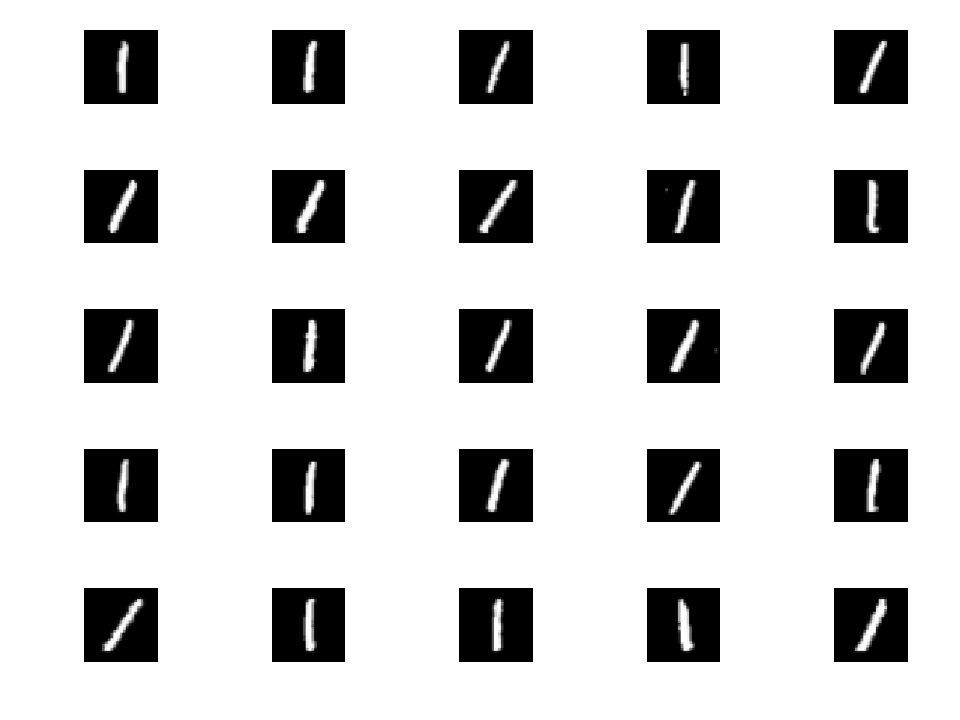
\includegraphics[width=6cm]{images/images_davae/mnist_small_distance}
		\caption{Statistiques de distance faible}
	\end{subfigure}
	\begin{subfigure}{6cm}
		\centering
\includegraphics[width=6cm]{images/images_davae/mnist_large_distance}
		\caption{Statistiques de distance élevées}
	\end{subfigure}
	\caption{Échantillons d'images provenant du jeu de données d'entraînement ayant des statistiques de distance faibles (a) et élevées (b) pour le scénario de test 3 ("Plus") du jeu de données \textit{MNIST}.}
	\label{fig:latentes_images_mnist}
\end{figure}

De cette manière, il est possible de conclure que nous nous retrouvons plutôt dans le premier scénario décrit (voir les deux scénarios décrits à la sous-section \ref{liste_scenarios}), soit celui où les représentations latentes des observations "normales" sont plus près de la $N(0,I)$. C'est donc le scénario inverse par rapport aux expérimentations faites sur \textit{ImageNet}. On peut d'ailleurs confirmer cette conclusion dans la figure \ref{fig:mnist_latent_stats}, où l'on peut voir que les vecteurs $\boldsymbol{\mu}$ et $\boldsymbol{\sigma}$ moyens des observations "normales" sont plus près des paramètres de moyenne et d'écart-type de la $N(0,I)$.

\begin{figure}[H]
	\centering
	\begin{subfigure}{12cm}
		\centering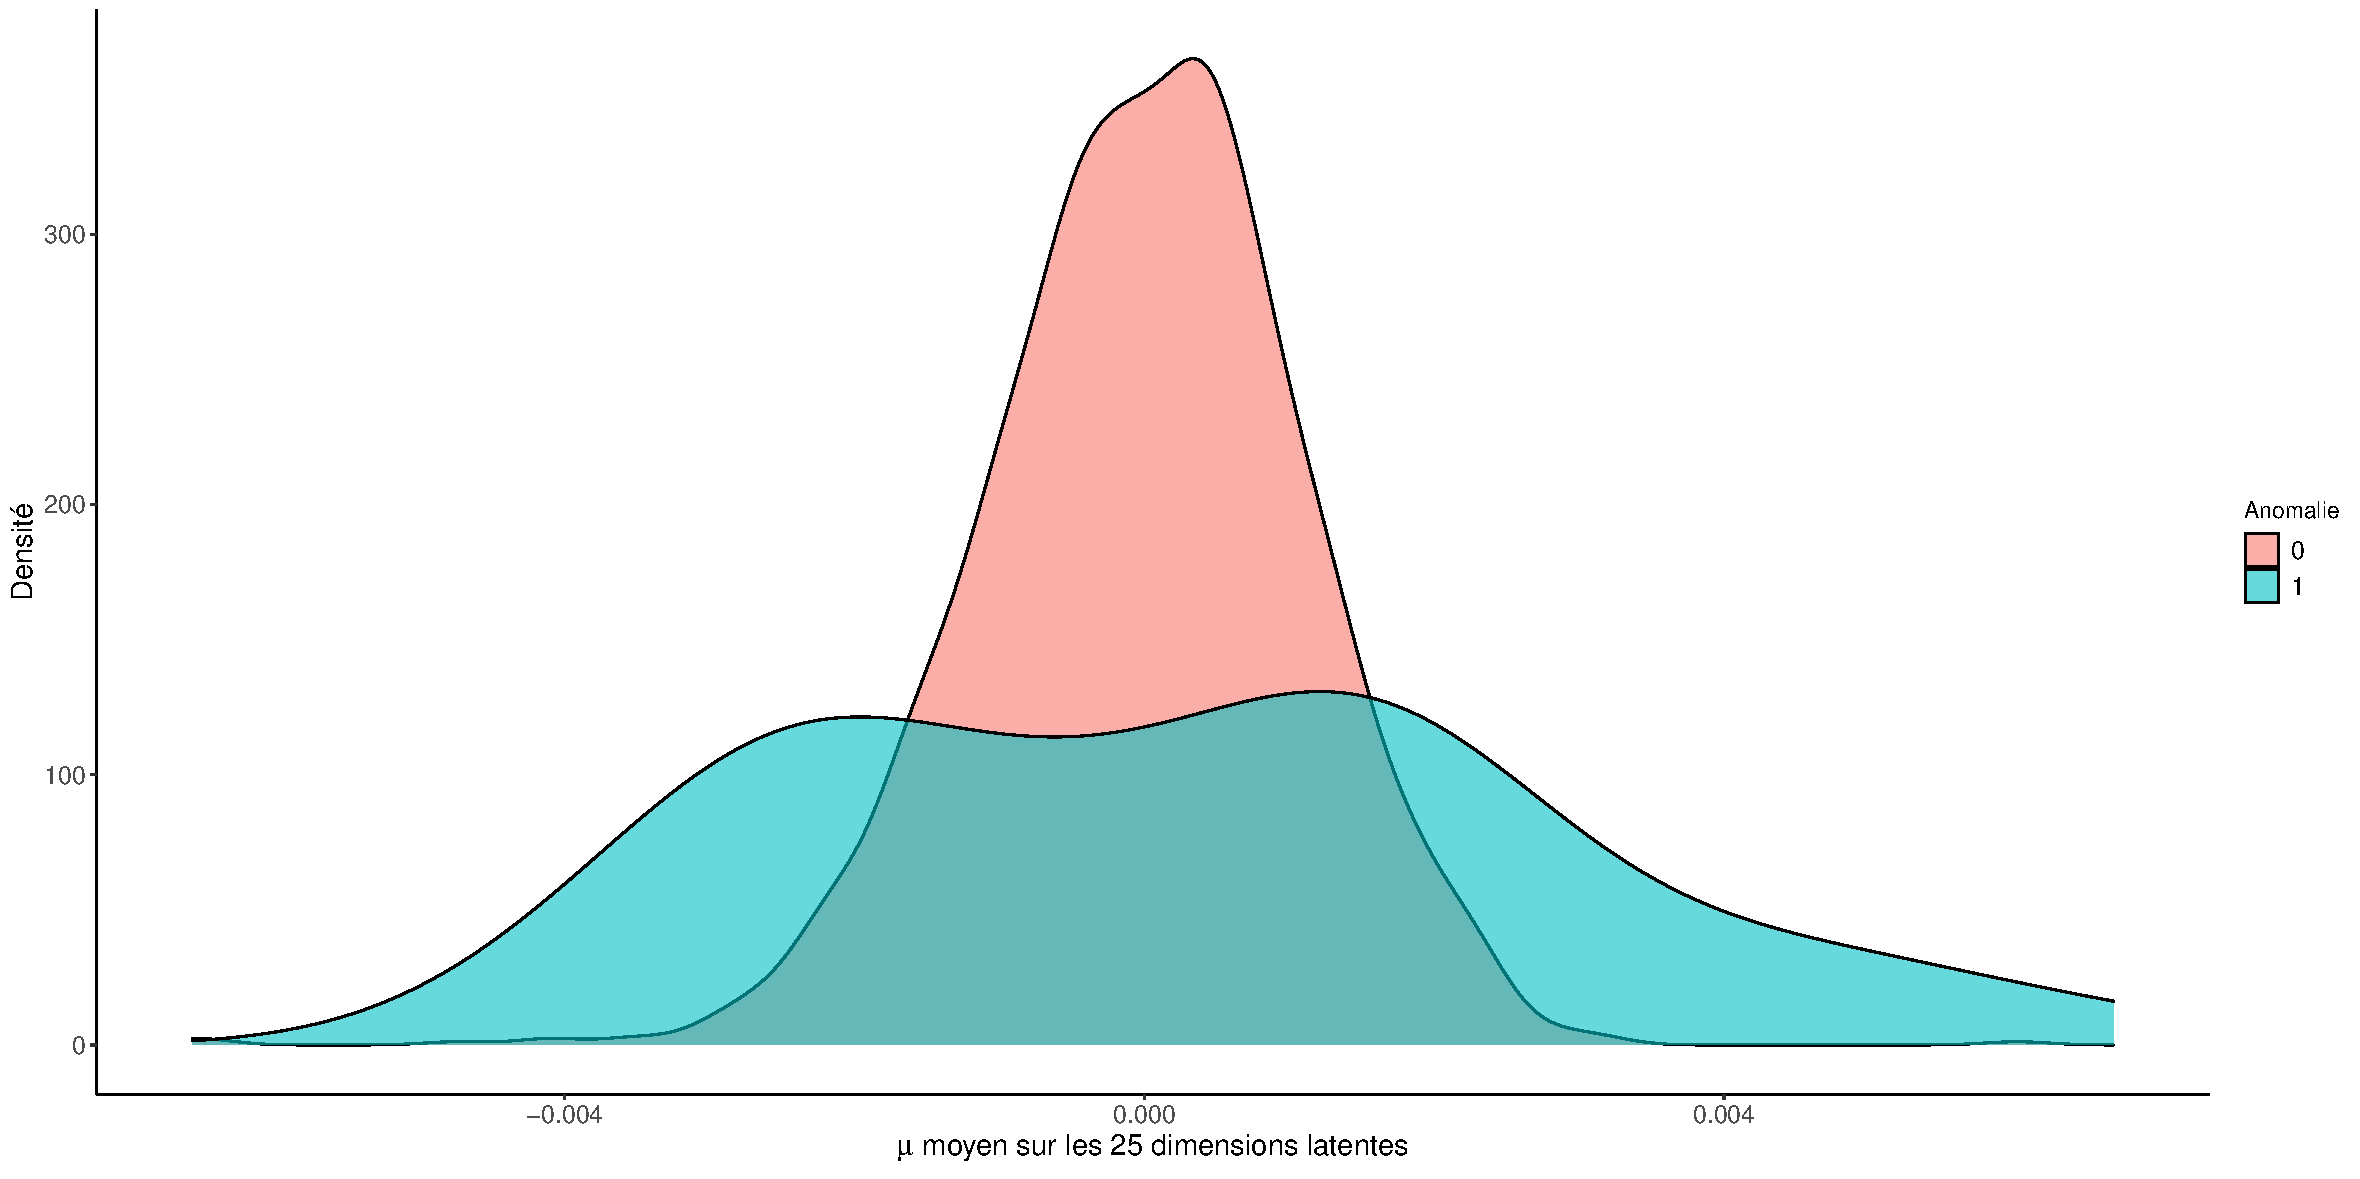
\includegraphics[width=12cm, height=6cm]{images/latent_stats/plot_mu_mnist}
		\caption{Distribution des $\boldsymbol{\mu}$ moyens}
	\end{subfigure}
	\begin{subfigure}{12cm}
		\centering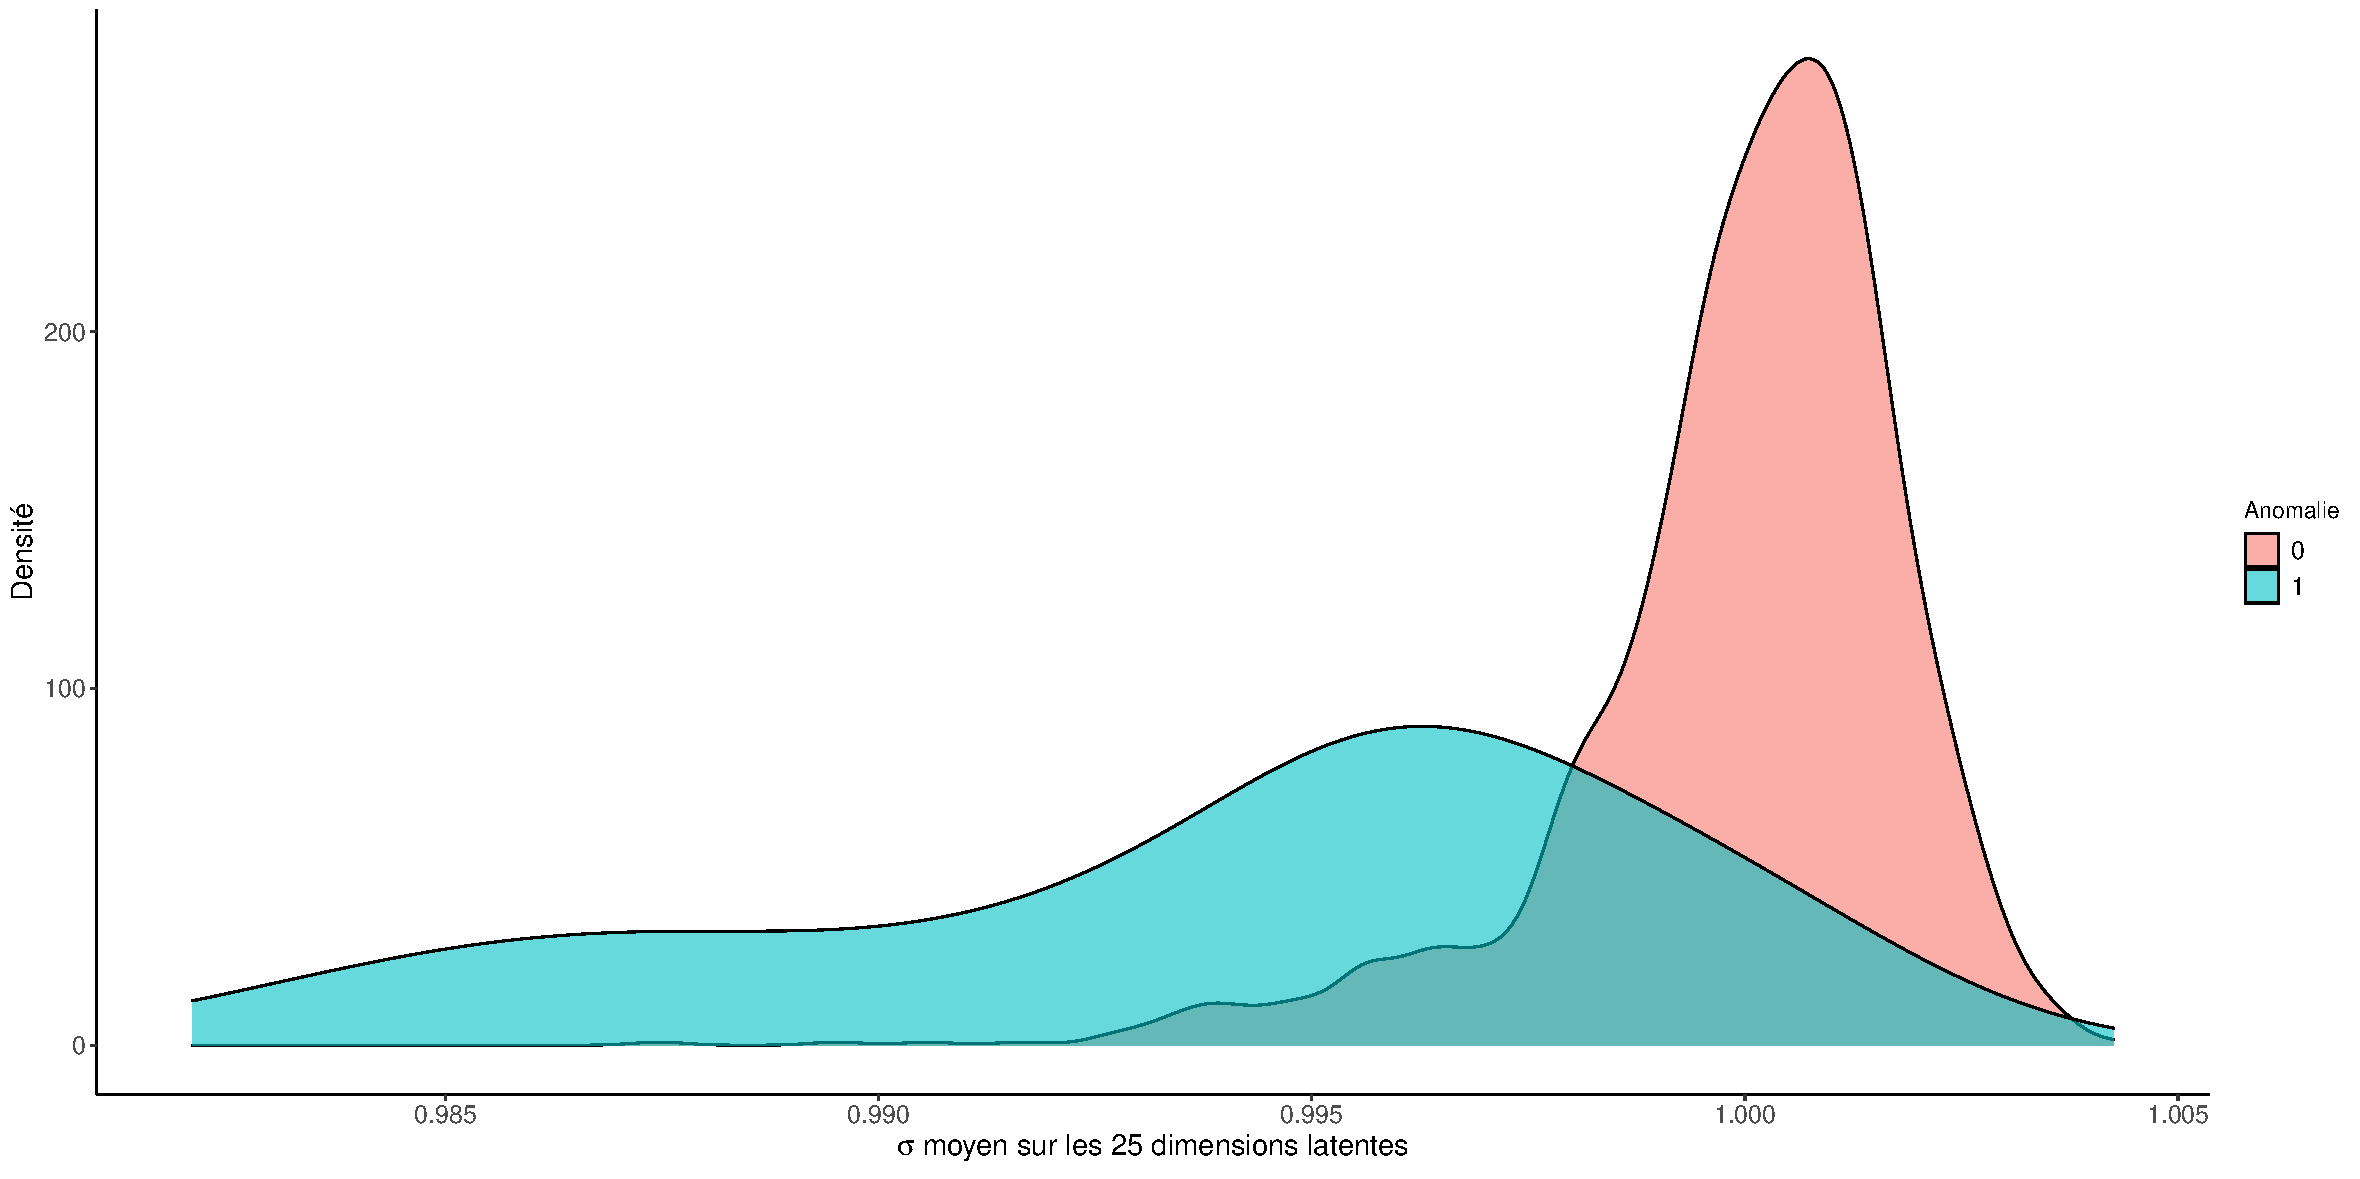
\includegraphics[width=12cm, height=6cm]{images/latent_stats/plot_sigma_mnist}
		\caption{Distribution des $\boldsymbol{\sigma}$ moyens}
	\end{subfigure}
	\caption{Moyenne des $\boldsymbol{\mu}$ et $\boldsymbol{\sigma}$ des représentations latentes du jeu de données d'entraînement sur le jeu de données \textit{MNIST}.}
	\label{fig:mnist_latent_stats}
\end{figure}

\begin{figure}[htb]
	\centering
	\centering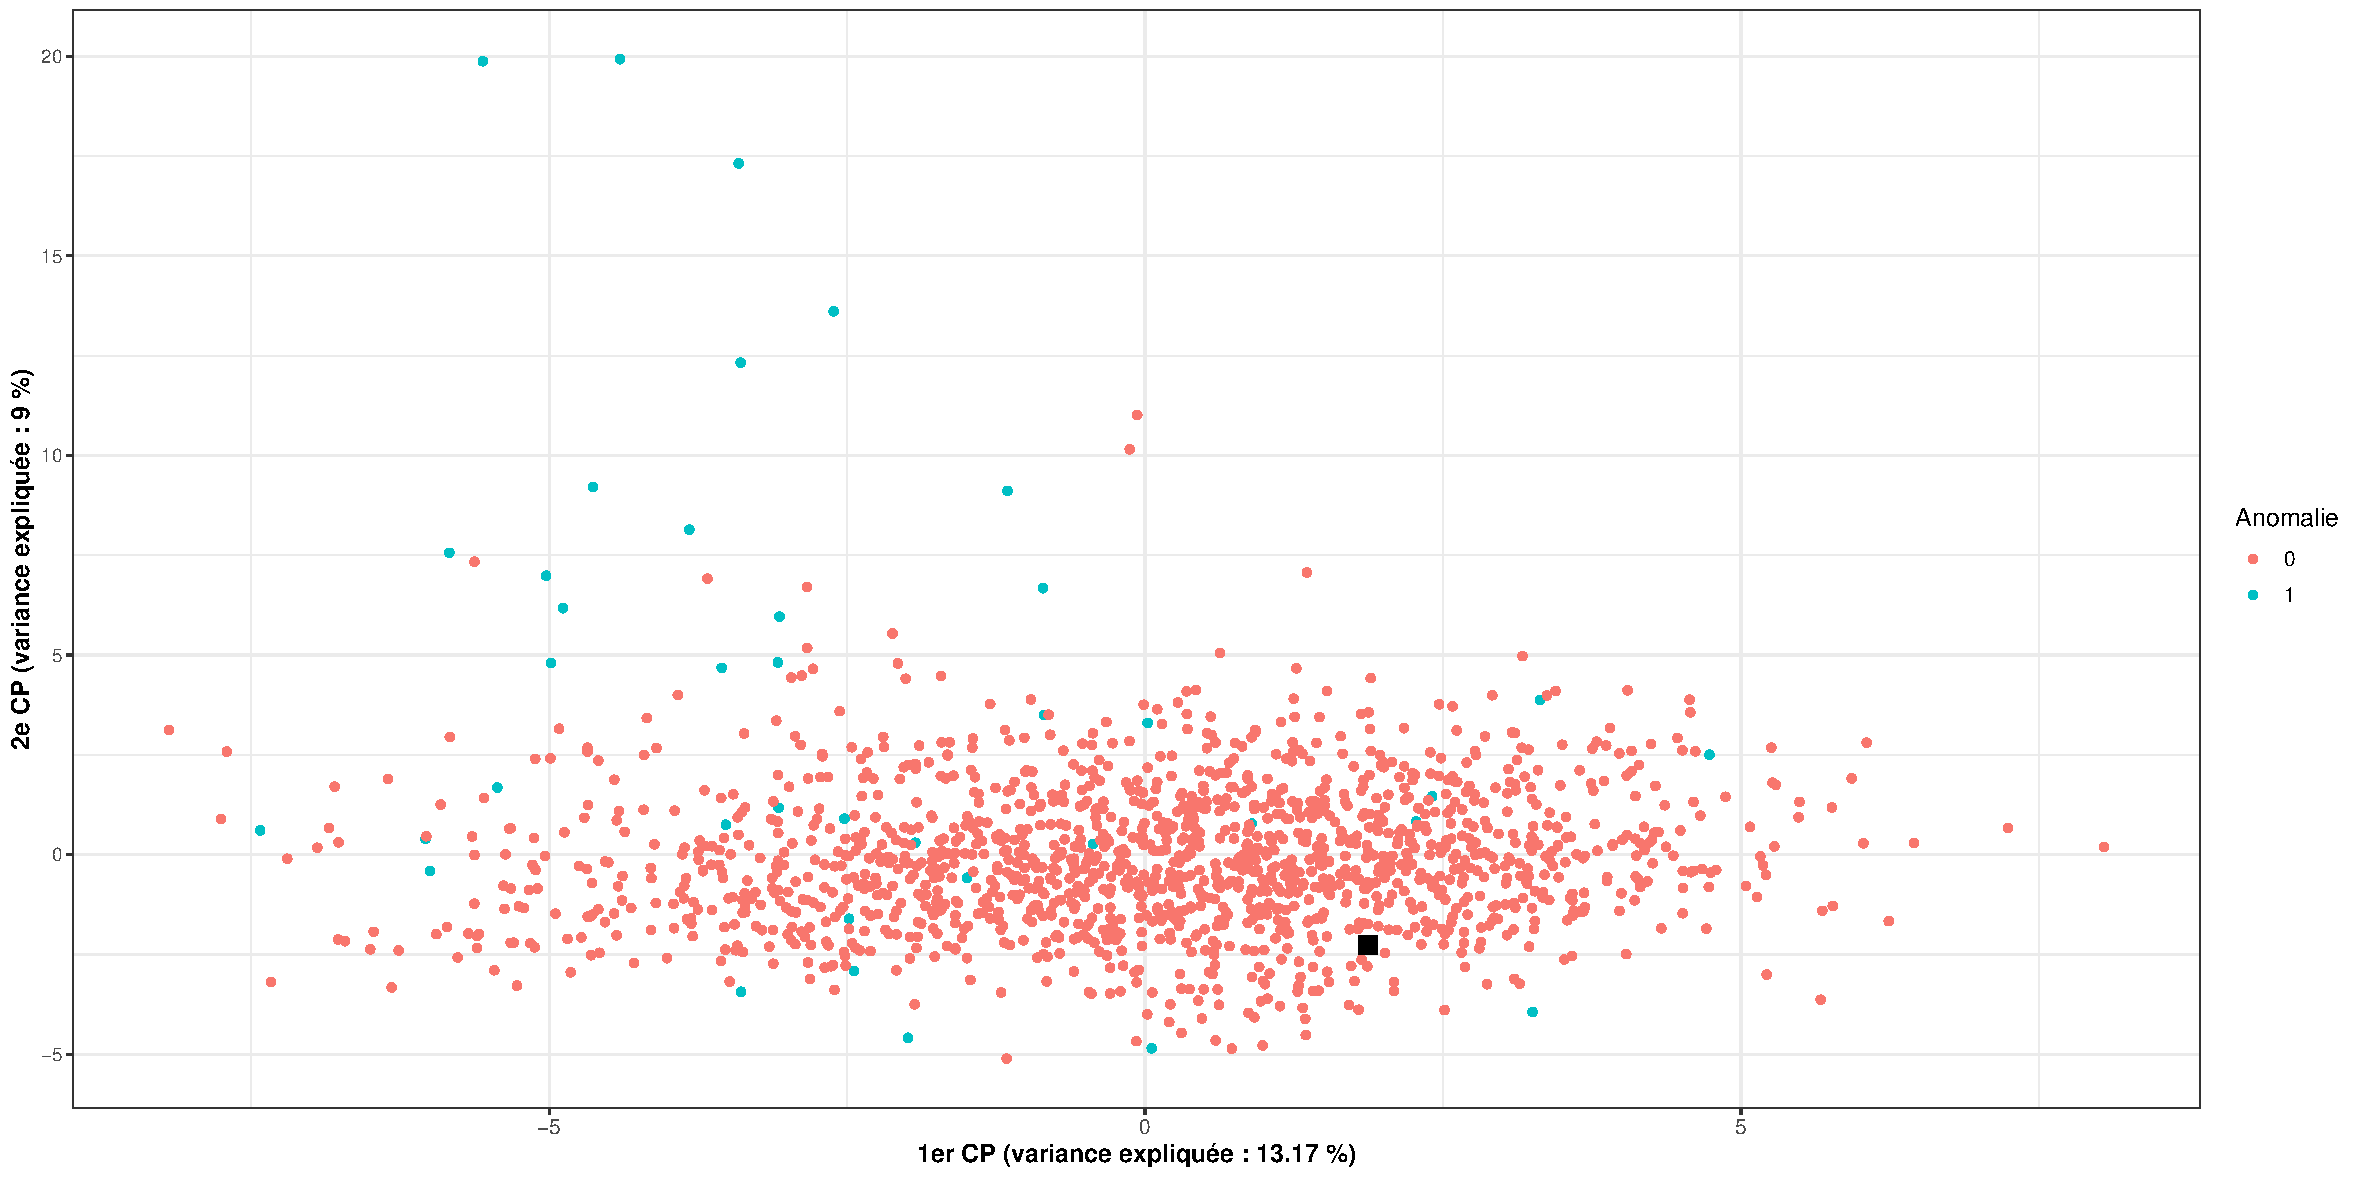
\includegraphics[width=\linewidth]{images/plot_pca_mnist}
	\caption{Graphique des \DIFdelbeginFL \DIFdelFL{2 }\DIFdelendFL \DIFaddbeginFL \DIFaddFL{deux }\DIFaddendFL premières composantes principales réalisé sur les vecteurs $\boldsymbol{\mu}$ et $\boldsymbol{\sigma}$ du jeu de données d'entraînement \textit{MNIST} appliqué sur le scénario de test 3 et le scénario de contamination "Plus".}
	\label{fig:pca_mnist}
\end{figure}

Dans la figure \ref{fig:pca_mnist}, on peut voir le résultat d'une analyse en composantes principales appliquée sur les vecteurs $\boldsymbol{\mu}$ et $\boldsymbol{\sigma}$. Cette figure nous permet de visualiser en \DIFdelbegin \DIFdel{2 }\DIFdelend \DIFaddbegin \DIFadd{deux }\DIFaddend dimensions les représentations latentes apprises sur le jeu de données d'entraînement du scénario de test 3 et du scénario de contamination "Plus". Si on compare avec la figure \ref{fig:pca_cars} qui fait référence au jeu de données \textit{ImageNet}, la séparation des anomalies et des observations "normales" est beaucoup moins évidente. Cependant, les \DIFdelbegin \DIFdel{2 }\DIFdelend \DIFaddbegin \DIFadd{deux }\DIFaddend premières composantes principales n'expliquent même pas 25\% de la variabilité totale de la représentation latente. En se basant sur cette projection, les "anomalies" semblent être plus éloignées du carré noir, qui représente la projection dans cet espace du point $(\boldsymbol{0_{m}}, \boldsymbol{1_{m}})$. Cette conclusion concorde avec l'analyse de la figure \ref{fig:mnist_latent_stats}. Étant donné que l'analyse en composantes principales ne permet pas de voir clairement la séparation des anomalies et des observations "normales" dans un espace en deux dimensions, nous avons exploré une autre avenue afin d'obtenir cette visualisation. Pour ce faire, nous avons fait un nouvel entraînement de la méthode DA-VAE, mais cette fois-ci avec seulement deux dimensions latentes (au lieu de 25). Cette configuration nous permettra de visualiser les vecteurs $\boldsymbol{\mu}$ et $\boldsymbol{\sigma}$ dans un espace à deux dimensions sans avoir à faire de réduction de \DIFdelbegin \DIFdel{dimensionnalités}\DIFdelend \DIFaddbegin \DIFadd{dimensionnalité}\DIFaddend . Dans la figure \ref{fig:mnist_latent_2d}, on peut désormais voir de manière plus évidente que les représentations latentes des observations "normales" sont plus près du point $(\boldsymbol{0_{m}}, \boldsymbol{1_{m}})$.

\begin{figure}[H]
	\centering
	\begin{subfigure}{6cm}
		\centering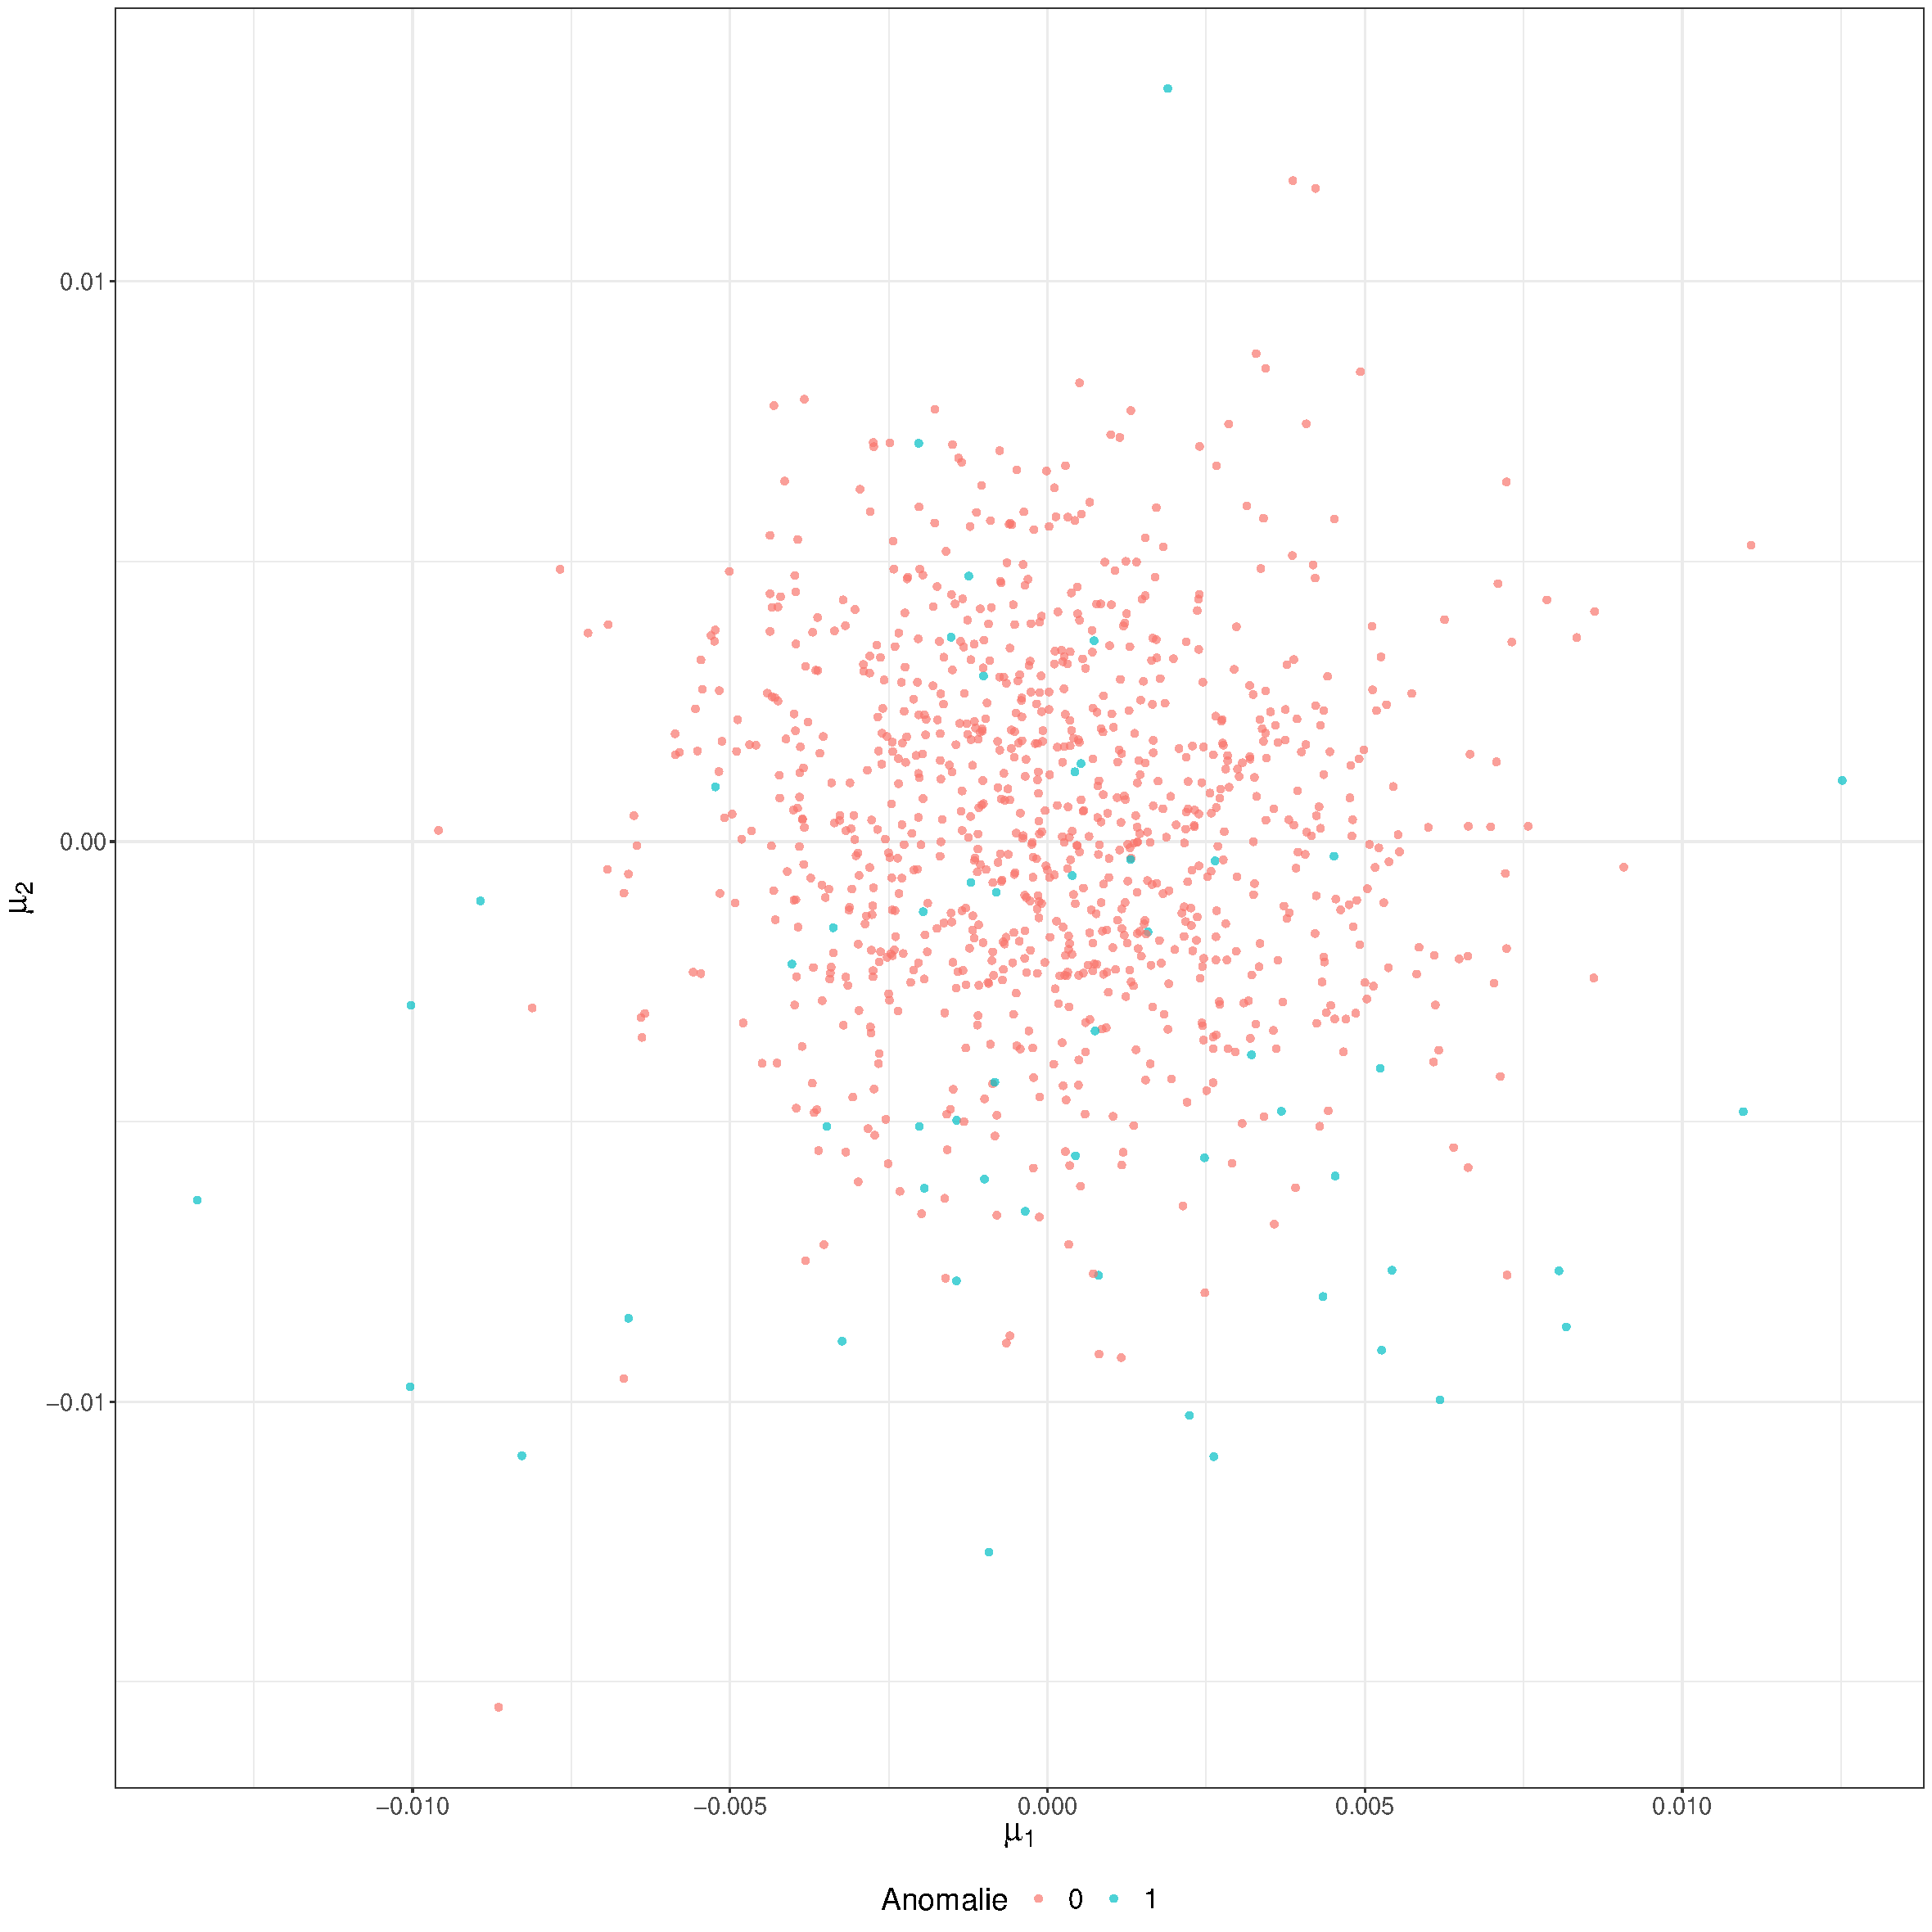
\includegraphics[width=6cm, height=6cm]{images/latent_stats/mnist_mu_2d}
		\caption{Distribution de $\mu_1$ et $\mu_2$}
	\end{subfigure}
	\begin{subfigure}{6cm}
		\centering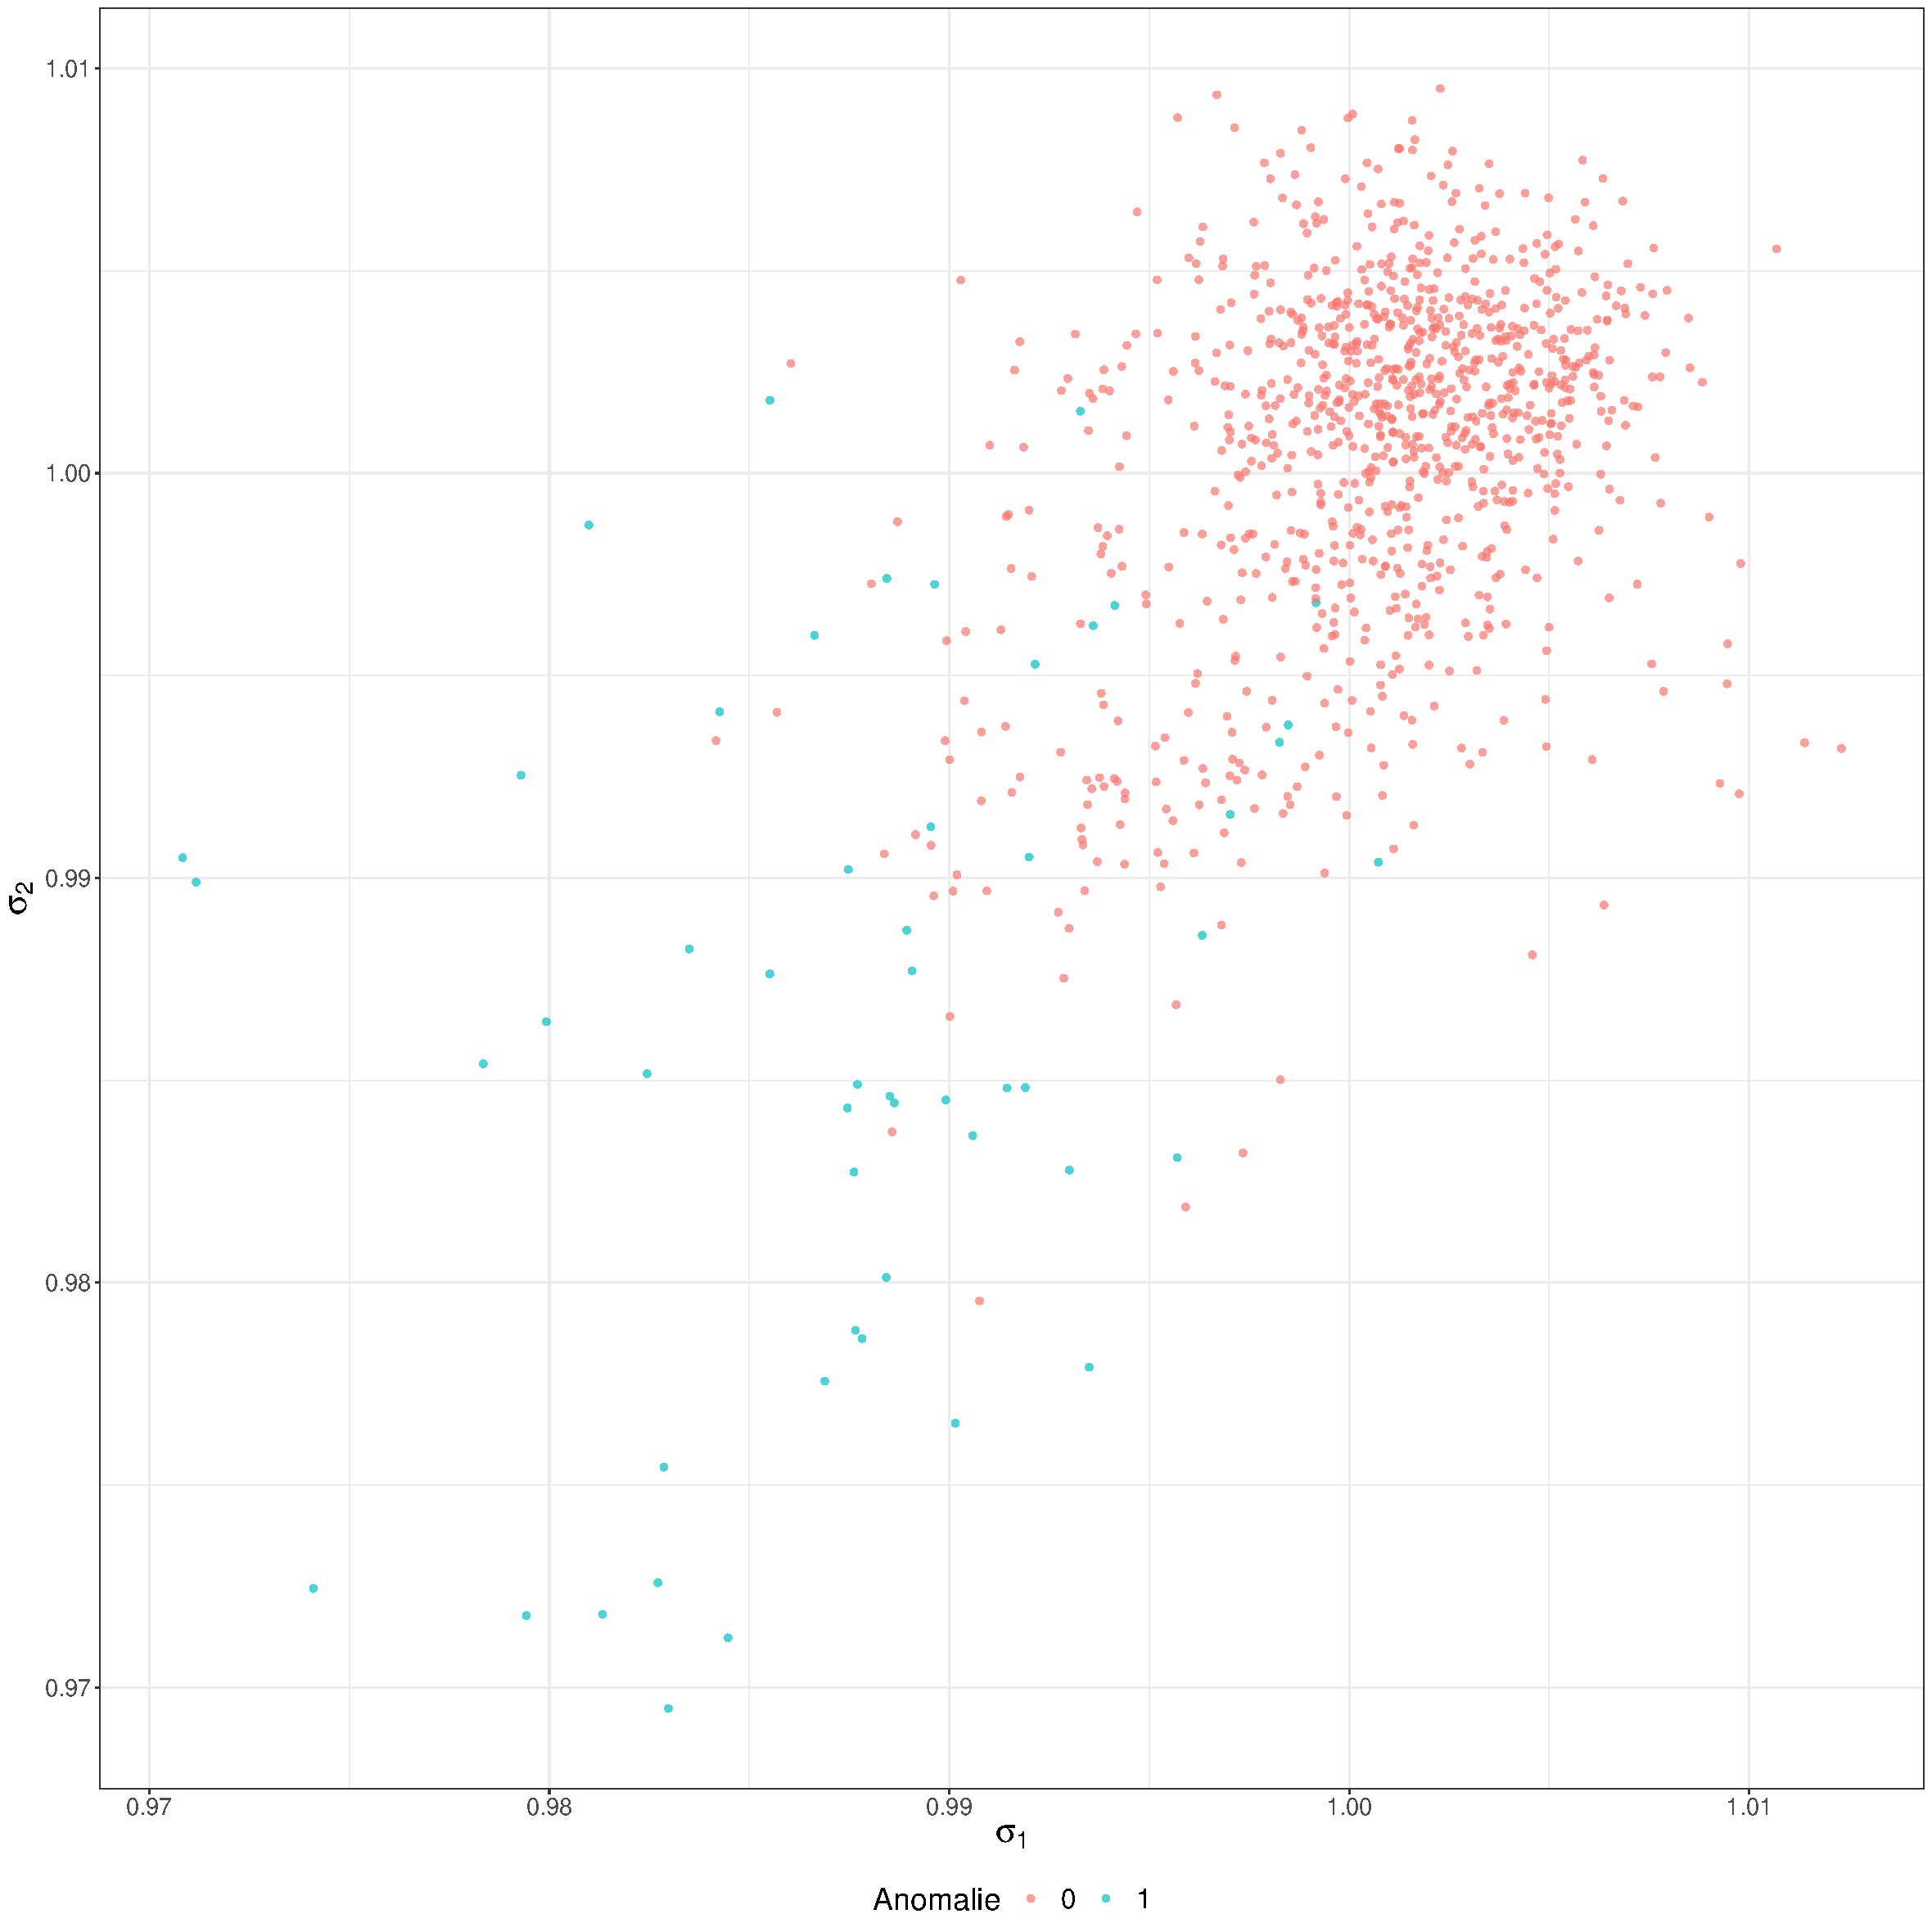
\includegraphics[width=6cm, height=6cm]{images/latent_stats/mnist_sigma_2d}
		\caption{Distribution de $\sigma_1$ et $\sigma_2$}
	\end{subfigure}
	\caption{Distribution des vecteurs $\boldsymbol{\mu}$ et $\boldsymbol{\sigma}$ pour le modèle DA-VAE entraîné avec un espace latent à deux dimensions sur le scénario de test 3 et le scénario de contamination "Égal" du jeu de données \textit{MNIST}.}
	\label{fig:mnist_latent_2d}
\end{figure}

Dans la figure \ref{fig:mnist_latent_2d}, nous avons utilisé comme exemple un entraînement réalisé sur scénario de test 3 avec le scénario de contamination "Égal". Afin de pouvoir mieux observer la distribution des points, nous avons conservé seulement 500 observations, choisies aléatoirement, du jeu de données d'entraînement. Comme nous l'avions remarqué dans la figure \ref{fig:mnist_latent_stats}, les deux classes semblent mieux séparées selon le vecteur latent $\boldsymbol{\sigma}$ plutôt que selon le vecteur latent $\boldsymbol{\mu}$.

\subsubsection{Analyse de la perte en entraînement}

Dans la figure \ref{fig:mnist_kld_perc}, on peut voir la composition de la perte à chacune des itérations de l'entraînement. On peut voir que la proportion de la composante de perte de Kullback-Leibler suit le même patron qu'à la figure \ref{fig:cars_kld_perc}. Cependant, la proportion atteint un maximum beaucoup plus élevé que dans le cas du jeu de données provenant de \textit{ImageNet}. Encore une fois, il est rassurant de voir que la composition réelle de la perte soit cohérente avec notre horaire établi pour l'hyperparamètre $\beta$. 

\begin{figure}[h]
	\centering
	\includegraphics[width=\linewidth]{images/kld_mnist_scenario_3.pdf}
	\caption{Pourcentage du critère de Kullback-Leibler dans la perte totale selon l'itération d'entraînement et le scénario de contamination. Ces résultats sont tirés du scénario de test 3, où le chiffre "1" est considéré comme la classe "normale" et tous les autres sont considérés dans la classe "anormale".}
	\label{fig:mnist_kld_perc}
\end{figure}

             % experimentations
\chapter*{Conclusion}           % ne pas numéroter
\label{chap:conclusion}         % étiquette pour renvois
\phantomsection\addcontentsline{toc}{chapter}{\nameref{chap:conclusion}} % inclure dans TdM

La détection d'anomalies est une tâche qui comporte généralement plusieurs défis en modélisation et en analyse de données. Ces défis, dont \DIFdelbegin \DIFdel{entres }\DIFdelend \DIFaddbegin \DIFadd{entre }\DIFaddend autres l'absence d'étiquettes pour l'entraînement, ont été mentionnés et décrits brièvement dans le chapitre d'\nameref{chap:introduction}. Notre objectif est de proposer une méthodologie qui permet d'identifier les images d'un jeu de données qui dévient de la normalité et qui s'apparentent donc à des anomalies. Nous souhaitons faire cette détection d'anomalies de manière non supervisée tout en simplifiant l'établissement du seuil nous permettant de catégoriser \DIFdelbegin \DIFdel{une observation }\DIFdelend \DIFaddbegin \DIFadd{si une observation est }\DIFaddend "normale" \DIFdelbegin \DIFdel{et une observation }\DIFdelend \DIFaddbegin \DIFadd{ou  }\DIFaddend "anormale". 

Dans ce mémoire, nous démontrons la pertinence d'utiliser des autoencodeurs variationnels pour faire face aux défis traditionnels reliés à la détection d'anomalies, tout en restant \DIFdelbegin \DIFdel{efficaces }\DIFdelend \DIFaddbegin \DIFadd{efficace }\DIFaddend dans un contexte où les données sont complexes, comme des images. Nous discutons également de différentes approches permettant de faire la détection d'anomalies, en mettant l'accent sur les méthodes \DIFdelbegin \DIFdel{d'}\DIFdelend \DIFaddbegin \DIFadd{basées sur des }\DIFaddend autoencodeurs qui sont bien adaptées pour traiter des images.

\DIFdelbegin \DIFdel{Dans les }\DIFdelend \DIFaddbegin \DIFadd{Suite aux }\DIFaddend expérimentations réalisées et présentées dans le chapitre \ref{chap:experiments}, nous sommes en mesure de conclure que notre approche produit des résultats performants autant sur des jeux de données d'images réelles que d'images simples. La valeur ajoutée de notre approche par rapport à d'autres méthodes est toutefois beaucoup plus évidente dans le cas d'images réelles. En effet, les performances obtenues par notre approche sur des images simples, comme \textit{MNIST}, ne sont généralement pas significativement meilleures ou pires que d'autres approches. En revanche, les performances en aire sous la courbe ROC, en précision et en rappel obtenues sur des images réelles plus complexes, comme \textit{ImageNet}, sont supérieures aux autres approches comparatives. Ces bonnes performances nous laissent croire que nous avons rempli notre objectif d'être en mesure de détecter des anomalies dans un ensemble d'images. De plus, la mise en place de notre niveau de filtration $\alpha$ nous permet d'avoir un seuil simple et intuitif à établir.


 Le facteur principal expliquant les bonnes performances obtenues sur des images réelles est l'utilisation d'un autoencodeur variationnel. En effet, cet algorithme d'apprentissage profond permet de représenter des données complexes dans une forme latente beaucoup plus simple et permet aussi de bien identifier des observations "normales". Un des avantages de notre approche est que les performances en détection d'anomalies demeurent élevées dans plusieurs scénarios différents: différentes complexités d'images, différentes proportions de contamination, etc. Un des points faibles de notre approche est que l'autoencodeur variationnel est un algorithme relativement complexe avec \DIFdelbegin \DIFdel{beaucoup d'}\DIFdelend \DIFaddbegin \DIFadd{plusieurs }\DIFaddend hyperparamètres. En effet, il faut déterminer \DIFdelbegin \DIFdel{entres }\DIFdelend \DIFaddbegin \DIFadd{entre }\DIFaddend autres le nombre de couches de l'autoencodeur, la taille des filtres, les fonctions d'activation, la taille de la dimension latente, etc. C'est d'ailleurs un point commun à la majorité des approches basées sur \DIFdelbegin \DIFdel{les }\DIFdelend \DIFaddbegin \DIFadd{des }\DIFaddend réseaux de neurones. Ensuite, un autre point faible de notre approche est qu'on doit réaliser une étape manuelle, après l'entraînement de l'autoencodeur, où l'on doit inspecter certaines observations pour voir si les représentations latentes des observations "normales" sont plus près ou plus éloignées de notre point de référence\DIFaddbegin \DIFadd{, en l'occurrence la loi $N(0,I)$}\DIFaddend . Cette étape fait en sorte que notre méthodologie n'est pas pleinement automatique.

À la lumière de nos résultats, notre approche pourrait être utilisée pour plusieurs applications ou situations réelles où l'on cherche à identifier des images "anormales". Prenons par exemple une situation où l'on \DIFdelbegin \DIFdel{bénéficie }\DIFdelend \DIFaddbegin \DIFadd{dispose }\DIFaddend d'un ensemble d'images propres pour lequel on sait qu'il n'y a pas d'\DIFdelbegin \DIFdel{anomalies ou de défectuosités}\DIFdelend \DIFaddbegin \DIFadd{anomalie ou de défectuosité}\DIFaddend . Supposons que dans le futur, on prévoit recevoir de nouvelles images qui sont supposées représenter la même chose que notre ensemble d'images propres, mais dont certaines de ces nouvelles images sont défectueuses où représentent quelque chose de complètement différent. Nous ne connaissons pas d'avance à quoi ces images défectueuses pourraient ressembler et n'avons aucun exemple d'image de la sorte sur lesquelles on pourrait faire un apprentissage. Notre approche permettrait donc de déterminer lesquelles de ces nouvelles images sont potentiellement défectueuses ou ne semblent pas représenter la même chose que notre ensemble d'images \DIFdelbegin \DIFdel{a priori}\DIFdelend \DIFaddbegin \textit{\DIFadd{a priori}}\DIFaddend . On pourrait également penser à des exemples d'applications où l'on cherche à nettoyer un jeu de données d'images. En effet, on pourrait commencer par valider et confirmer un sous-ensemble d'images propres dans notre jeu de données complet. Ensuite, on pourrait utiliser ce sous-ensemble comme jeu de données d'entraînement pour notre approche. Finalement, on pourrait utiliser le reste du jeu de données comme jeu de données de test et ainsi valider si des images "anormales" font \DIFdelbegin \DIFdel{parties }\DIFdelend \DIFaddbegin \DIFadd{partie }\DIFaddend de notre ensemble global. Cela reviendrait donc à utiliser notre approche comme technique de nettoyage de données.

Dans le futur, il serait intéressant de voir si des variations de l'autoencodeur variationnel pourraient donner de meilleurs résultats en détection d'anomalies. Parmi les possibilités de variations, il serait intéressant de voir si une autre loi que la $N(0,I)$ pourrait être utilisée comme loi \DIFdelbegin \DIFdel{a priori }\DIFdelend \DIFaddbegin \textit{\DIFadd{a priori}} \DIFaddend de la représentation latente et définir une statistique de distance sur cette nouvelle représentation latente. L'objectif serait d'explorer d'autres lois qui pourraient mieux discriminer des observations "normales" d'un petit groupe d'observations "anormales". Ensuite, il serait pertinent de voir s'il est possible de mieux contrôler les \DIFdelbegin \DIFdel{2 }\DIFdelend \DIFaddbegin \DIFadd{deux }\DIFaddend composantes de perte de l'autoencodeur variationnel. De ce fait, nous avons remarqué que ces deux composantes ont parfois des échelles très différentes, ce qui affecte l'entraînement de l'autoencodeur et la composition de la représentation latente. Dans ce mémoire, nous avons fait plusieurs essais et avons utilisé l'hyperparamètre $\beta$  pour modifier la pondération des deux composantes de perte. Cette approche requiert donc \DIFdelbegin \DIFdel{beaucoup }\DIFdelend \DIFaddbegin \DIFadd{plusieurs cycles }\DIFaddend d'essais et erreurs, ce qui n'est pas optimal. Finalement, il serait également intéressant de voir s'il est possible de faire en sorte que les représentations latentes des anomalies se comportent toujours de la même manière par rapport à un point de référence, soit la distribution $N(0,I)$ dans notre cas. En effet, nous avons remarqué que selon la nature des données, les représentations latentes des anomalies se retrouvaient dans certains cas plus près de la $N(0,I)$ et dans certains cas  plus éloignées de la $N(0,I)$. Ce constat ajoute une étape manuelle pour mettre en place notre méthodologie, ce qui rend l'approche moins automatique et plus difficile à appliquer dans la pratique. Il serait \DIFdelbegin \DIFdel{également }\DIFdelend pertinent de voir si un \DIFdelbegin \DIFdel{meilleur }\DIFdelend point de référence \DIFdelbegin \DIFdel{, }\DIFdelend autre que la $N(0,I)$ \DIFdelbegin \DIFdel{, pourrait être testé}\DIFdelend \DIFaddbegin \DIFadd{pourrait améliorer la méthode}\DIFaddend . Au final, nous pouvons conclure que l'autoencodeur variationnel possède des propriétés intéressantes, via l'apprentissage d'une représentation latente, pour faire de la détection d'anomalies sur des données complexes comme des images.


            % conclusion

\appendix                       % annexes le cas échéant

%\chapter{<Titre de l'annexe>}     % numérotée
\label{chap:}                   % étiquette pour renvois (à compléter!)

<Texte de l'annexe.>
                % annexe A

\bibliography{bibliography}                 % production de la bibliographie

\end{document}
